% Options for packages loaded elsewhere
\PassOptionsToPackage{unicode}{hyperref}
\PassOptionsToPackage{hyphens}{url}
\PassOptionsToPackage{dvipsnames,svgnames,x11names}{xcolor}
%
\documentclass[
  letterpaper,
  krantz2]{{[}./krantz{]}}

\usepackage{amsmath,amssymb}
\usepackage{iftex}
\ifPDFTeX
  \usepackage[T1]{fontenc}
  \usepackage[utf8]{inputenc}
  \usepackage{textcomp} % provide euro and other symbols
\else % if luatex or xetex
  \usepackage{unicode-math}
  \defaultfontfeatures{Scale=MatchLowercase}
  \defaultfontfeatures[\rmfamily]{Ligatures=TeX,Scale=1}
\fi
\usepackage{lmodern}
\ifPDFTeX\else  
    % xetex/luatex font selection
\fi
% Use upquote if available, for straight quotes in verbatim environments
\IfFileExists{upquote.sty}{\usepackage{upquote}}{}
\IfFileExists{microtype.sty}{% use microtype if available
  \usepackage[]{microtype}
  \UseMicrotypeSet[protrusion]{basicmath} % disable protrusion for tt fonts
}{}
\makeatletter
\@ifundefined{KOMAClassName}{% if non-KOMA class
  \IfFileExists{parskip.sty}{%
    \usepackage{parskip}
  }{% else
    \setlength{\parindent}{0pt}
    \setlength{\parskip}{6pt plus 2pt minus 1pt}}
}{% if KOMA class
  \KOMAoptions{parskip=half}}
\makeatother
\usepackage{xcolor}
\setlength{\emergencystretch}{3em} % prevent overfull lines
\setcounter{secnumdepth}{5}
% Make \paragraph and \subparagraph free-standing
\makeatletter
\ifx\paragraph\undefined\else
  \let\oldparagraph\paragraph
  \renewcommand{\paragraph}{
    \@ifstar
      \xxxParagraphStar
      \xxxParagraphNoStar
  }
  \newcommand{\xxxParagraphStar}[1]{\oldparagraph*{#1}\mbox{}}
  \newcommand{\xxxParagraphNoStar}[1]{\oldparagraph{#1}\mbox{}}
\fi
\ifx\subparagraph\undefined\else
  \let\oldsubparagraph\subparagraph
  \renewcommand{\subparagraph}{
    \@ifstar
      \xxxSubParagraphStar
      \xxxSubParagraphNoStar
  }
  \newcommand{\xxxSubParagraphStar}[1]{\oldsubparagraph*{#1}\mbox{}}
  \newcommand{\xxxSubParagraphNoStar}[1]{\oldsubparagraph{#1}\mbox{}}
\fi
\makeatother

\usepackage{color}
\usepackage{fancyvrb}
\newcommand{\VerbBar}{|}
\newcommand{\VERB}{\Verb[commandchars=\\\{\}]}
\DefineVerbatimEnvironment{Highlighting}{Verbatim}{commandchars=\\\{\}}
% Add ',fontsize=\small' for more characters per line
\usepackage{framed}
\definecolor{shadecolor}{RGB}{241,243,245}
\newenvironment{Shaded}{\begin{snugshade}}{\end{snugshade}}
\newcommand{\AlertTok}[1]{\textcolor[rgb]{0.68,0.00,0.00}{#1}}
\newcommand{\AnnotationTok}[1]{\textcolor[rgb]{0.37,0.37,0.37}{#1}}
\newcommand{\AttributeTok}[1]{\textcolor[rgb]{0.40,0.45,0.13}{#1}}
\newcommand{\BaseNTok}[1]{\textcolor[rgb]{0.68,0.00,0.00}{#1}}
\newcommand{\BuiltInTok}[1]{\textcolor[rgb]{0.00,0.23,0.31}{#1}}
\newcommand{\CharTok}[1]{\textcolor[rgb]{0.13,0.47,0.30}{#1}}
\newcommand{\CommentTok}[1]{\textcolor[rgb]{0.37,0.37,0.37}{#1}}
\newcommand{\CommentVarTok}[1]{\textcolor[rgb]{0.37,0.37,0.37}{\textit{#1}}}
\newcommand{\ConstantTok}[1]{\textcolor[rgb]{0.56,0.35,0.01}{#1}}
\newcommand{\ControlFlowTok}[1]{\textcolor[rgb]{0.00,0.23,0.31}{\textbf{#1}}}
\newcommand{\DataTypeTok}[1]{\textcolor[rgb]{0.68,0.00,0.00}{#1}}
\newcommand{\DecValTok}[1]{\textcolor[rgb]{0.68,0.00,0.00}{#1}}
\newcommand{\DocumentationTok}[1]{\textcolor[rgb]{0.37,0.37,0.37}{\textit{#1}}}
\newcommand{\ErrorTok}[1]{\textcolor[rgb]{0.68,0.00,0.00}{#1}}
\newcommand{\ExtensionTok}[1]{\textcolor[rgb]{0.00,0.23,0.31}{#1}}
\newcommand{\FloatTok}[1]{\textcolor[rgb]{0.68,0.00,0.00}{#1}}
\newcommand{\FunctionTok}[1]{\textcolor[rgb]{0.28,0.35,0.67}{#1}}
\newcommand{\ImportTok}[1]{\textcolor[rgb]{0.00,0.46,0.62}{#1}}
\newcommand{\InformationTok}[1]{\textcolor[rgb]{0.37,0.37,0.37}{#1}}
\newcommand{\KeywordTok}[1]{\textcolor[rgb]{0.00,0.23,0.31}{\textbf{#1}}}
\newcommand{\NormalTok}[1]{\textcolor[rgb]{0.00,0.23,0.31}{#1}}
\newcommand{\OperatorTok}[1]{\textcolor[rgb]{0.37,0.37,0.37}{#1}}
\newcommand{\OtherTok}[1]{\textcolor[rgb]{0.00,0.23,0.31}{#1}}
\newcommand{\PreprocessorTok}[1]{\textcolor[rgb]{0.68,0.00,0.00}{#1}}
\newcommand{\RegionMarkerTok}[1]{\textcolor[rgb]{0.00,0.23,0.31}{#1}}
\newcommand{\SpecialCharTok}[1]{\textcolor[rgb]{0.37,0.37,0.37}{#1}}
\newcommand{\SpecialStringTok}[1]{\textcolor[rgb]{0.13,0.47,0.30}{#1}}
\newcommand{\StringTok}[1]{\textcolor[rgb]{0.13,0.47,0.30}{#1}}
\newcommand{\VariableTok}[1]{\textcolor[rgb]{0.07,0.07,0.07}{#1}}
\newcommand{\VerbatimStringTok}[1]{\textcolor[rgb]{0.13,0.47,0.30}{#1}}
\newcommand{\WarningTok}[1]{\textcolor[rgb]{0.37,0.37,0.37}{\textit{#1}}}

\providecommand{\tightlist}{%
  \setlength{\itemsep}{0pt}\setlength{\parskip}{0pt}}\usepackage{longtable,booktabs,array}
\usepackage{multirow}
\usepackage{calc} % for calculating minipage widths
% Correct order of tables after \paragraph or \subparagraph
\usepackage{etoolbox}
\makeatletter
\patchcmd\longtable{\par}{\if@noskipsec\mbox{}\fi\par}{}{}
\makeatother
% Allow footnotes in longtable head/foot
\IfFileExists{footnotehyper.sty}{\usepackage{footnotehyper}}{\usepackage{footnote}}
\makesavenoteenv{longtable}
\usepackage{graphicx}
\makeatletter
\def\maxwidth{\ifdim\Gin@nat@width>\linewidth\linewidth\else\Gin@nat@width\fi}
\def\maxheight{\ifdim\Gin@nat@height>\textheight\textheight\else\Gin@nat@height\fi}
\makeatother
% Scale images if necessary, so that they will not overflow the page
% margins by default, and it is still possible to overwrite the defaults
% using explicit options in \includegraphics[width, height, ...]{}
\setkeys{Gin}{width=\maxwidth,height=\maxheight,keepaspectratio}
% Set default figure placement to htbp
\makeatletter
\def\fps@figure{htbp}
\makeatother
% definitions for citeproc citations
\NewDocumentCommand\citeproctext{}{}
\NewDocumentCommand\citeproc{mm}{%
  \begingroup\def\citeproctext{#2}\cite{#1}\endgroup}
\makeatletter
 % allow citations to break across lines
 \let\@cite@ofmt\@firstofone
 % avoid brackets around text for \cite:
 \def\@biblabel#1{}
 \def\@cite#1#2{{#1\if@tempswa , #2\fi}}
\makeatother
\newlength{\cslhangindent}
\setlength{\cslhangindent}{1.5em}
\newlength{\csllabelwidth}
\setlength{\csllabelwidth}{3em}
\newenvironment{CSLReferences}[2] % #1 hanging-indent, #2 entry-spacing
 {\begin{list}{}{%
  \setlength{\itemindent}{0pt}
  \setlength{\leftmargin}{0pt}
  \setlength{\parsep}{0pt}
  % turn on hanging indent if param 1 is 1
  \ifodd #1
   \setlength{\leftmargin}{\cslhangindent}
   \setlength{\itemindent}{-1\cslhangindent}
  \fi
  % set entry spacing
  \setlength{\itemsep}{#2\baselineskip}}}
 {\end{list}}
\usepackage{calc}
\newcommand{\CSLBlock}[1]{\hfill\break\parbox[t]{\linewidth}{\strut\ignorespaces#1\strut}}
\newcommand{\CSLLeftMargin}[1]{\parbox[t]{\csllabelwidth}{\strut#1\strut}}
\newcommand{\CSLRightInline}[1]{\parbox[t]{\linewidth - \csllabelwidth}{\strut#1\strut}}
\newcommand{\CSLIndent}[1]{\hspace{\cslhangindent}#1}

\usepackage{makeidx}
\makeindex
\documentclass{./krantz}
\makeatletter
\@ifpackageloaded{tcolorbox}{}{\usepackage[skins,breakable]{tcolorbox}}
\@ifpackageloaded{fontawesome5}{}{\usepackage{fontawesome5}}
\definecolor{quarto-callout-color}{HTML}{909090}
\definecolor{quarto-callout-note-color}{HTML}{0758E5}
\definecolor{quarto-callout-important-color}{HTML}{CC1914}
\definecolor{quarto-callout-warning-color}{HTML}{EB9113}
\definecolor{quarto-callout-tip-color}{HTML}{00A047}
\definecolor{quarto-callout-caution-color}{HTML}{FC5300}
\definecolor{quarto-callout-color-frame}{HTML}{acacac}
\definecolor{quarto-callout-note-color-frame}{HTML}{4582ec}
\definecolor{quarto-callout-important-color-frame}{HTML}{d9534f}
\definecolor{quarto-callout-warning-color-frame}{HTML}{f0ad4e}
\definecolor{quarto-callout-tip-color-frame}{HTML}{02b875}
\definecolor{quarto-callout-caution-color-frame}{HTML}{fd7e14}
\makeatother
\makeatletter
\@ifpackageloaded{bookmark}{}{\usepackage{bookmark}}
\makeatother
\makeatletter
\@ifpackageloaded{caption}{}{\usepackage{caption}}
\AtBeginDocument{%
\ifdefined\contentsname
  \renewcommand*\contentsname{Indice}
\else
  \newcommand\contentsname{Indice}
\fi
\ifdefined\listfigurename
  \renewcommand*\listfigurename{Elenco delle Figure}
\else
  \newcommand\listfigurename{Elenco delle Figure}
\fi
\ifdefined\listtablename
  \renewcommand*\listtablename{Elenco delle Tabelle}
\else
  \newcommand\listtablename{Elenco delle Tabelle}
\fi
\ifdefined\figurename
  \renewcommand*\figurename{Figura}
\else
  \newcommand\figurename{Figura}
\fi
\ifdefined\tablename
  \renewcommand*\tablename{Tabella}
\else
  \newcommand\tablename{Tabella}
\fi
}
\@ifpackageloaded{float}{}{\usepackage{float}}
\floatstyle{ruled}
\@ifundefined{c@chapter}{\newfloat{codelisting}{h}{lop}}{\newfloat{codelisting}{h}{lop}[chapter]}
\floatname{codelisting}{Lista}
\newcommand*\listoflistings{\listof{codelisting}{Elenco degli Elenchi}}
\makeatother
\makeatletter
\makeatother
\makeatletter
\@ifpackageloaded{caption}{}{\usepackage{caption}}
\@ifpackageloaded{subcaption}{}{\usepackage{subcaption}}
\makeatother
\makeatletter
\@ifpackageloaded{tcolorbox}{}{\usepackage[skins,breakable]{tcolorbox}}
\makeatother
\makeatletter
\@ifundefined{shadecolor}{\definecolor{shadecolor}{HTML}{f2f2f2}}{}
\makeatother
\makeatletter
\@ifundefined{codebgcolor}{\definecolor{codebgcolor}{HTML}{f2f2f2}}{}
\makeatother
\makeatletter
\ifdefined\Shaded\renewenvironment{Shaded}{\begin{tcolorbox}[boxrule=0pt, enhanced, breakable, frame hidden, sharp corners, borderline west={3pt}{0pt}{shadecolor}, colback={codebgcolor}]}{\end{tcolorbox}}\fi
\makeatother

\ifLuaTeX
\usepackage[bidi=basic]{babel}
\else
\usepackage[bidi=default]{babel}
\fi
\babelprovide[main,import]{italian}
% get rid of language-specific shorthands (see #6817):
\let\LanguageShortHands\languageshorthands
\def\languageshorthands#1{}
\ifLuaTeX
  \usepackage{selnolig}  % disable illegal ligatures
\fi
\usepackage{bookmark}

\IfFileExists{xurl.sty}{\usepackage{xurl}}{} % add URL line breaks if available
\urlstyle{same} % disable monospaced font for URLs
\hypersetup{
  pdftitle={Data Science per Psicologi},
  pdfauthor={Corrado Caudek},
  pdflang={it},
  colorlinks=true,
  linkcolor={black},
  filecolor={Maroon},
  citecolor={Blue},
  urlcolor={blue},
  pdfcreator={LaTeX via pandoc}}


\title{Data Science per Psicologi}
\usepackage{etoolbox}
\makeatletter
\providecommand{\subtitle}[1]{% add subtitle to \maketitle
  \apptocmd{\@title}{\par {\large #1 \par}}{}{}
}
\makeatother
\subtitle{Con applicazioni in Python e R}
\author{Corrado Caudek}
\date{2024-10-13}

\begin{document}
\maketitle


\bookmarksetup{startatroot}

\chapter*{Benvenuti}\label{benvenuti}
\addcontentsline{toc}{chapter}{Benvenuti}

\markboth{Benvenuti}{Benvenuti}

Questo sito web è dedicato al materiale didattico dell'insegnamento di
\href{https://www.unifi.it/index.php?module=ofform2&mode=1&cmd=3&AA=2023&afId=689762}{Psicometria}
(A.A. 2024/2025), rivolto agli studenti del primo anno del
\href{https://www.psicologia.unifi.it/vp-130-scienze-e-tecniche-psicologiche-l-24.html}{Corso
di Laurea in Scienze e Tecniche Psicologiche}
dell'\href{https://www.unifi.it/}{Università degli Studi di Firenze}.

Il corso è strutturato per fornire agli studenti una formazione teorica
e pratica approfondita nell'inferenza statistica, enfatizzando
particolarmente le applicazioni pratiche attraverso la programmazione.
Attraverso esercitazioni guidate, gli studenti impareranno a manipolare
e analizzare dati psicologici utilizzando Python, acquisendo così le
competenze necessarie per prendere decisioni informate e realizzare
interpretazioni precise nei loro progetti di modellazione.

Il programma copre un ampio spettro di tecniche, partendo dall'analisi
descrittiva per arrivare fino ai modelli gerarchici avanzati. Si pone un
forte accento sull'inferenza causale, approcciata da una prospettiva
bayesiana, includendo l'uso di Grafi Aciclici Diretti (DAG) per
esplorare in modo approfondito le relazioni causali. L'intento è di
andare oltre i limiti della modellazione lineare tradizionale, mostrando
come integrare efficacemente i modelli psicologici avanzati nell'analisi
statistica.

\section*{Informazioni
sull'insegnamento}\label{informazioni-sullinsegnamento}
\addcontentsline{toc}{section}{Informazioni sull'insegnamento}

\markright{Informazioni sull'insegnamento}

\begin{itemize}
\tightlist
\item
  \textbf{Codice}: B000286 - PSICOMETRIA
\item
  \textbf{Modulo}: B000286 - PSICOMETRIA (Cognomi L-Z)
\item
  \textbf{Corso di laurea}: Scienze e Tecniche Psicologiche
\item
  \textbf{Anno Accademico}: 2024-2025
\item
  \textbf{Materiali didattici}: È sufficiente disporre di un
  laptop/computer funzionante. Tutti i materiali didattici e il software
  necessario sono forniti gratuitamente a tutti gli studenti, senza
  richiedere alcun acquisto.
\item
  \textbf{Calendario}: Il corso si terrà dal 3 marzo al 31 maggio 2025.
\item
  \textbf{Orario delle lezioni}: Le lezioni si svolgeranno il lunedì e
  il martedì dalle 8:30 alle 10:30 e il giovedì dalle 11:30 alle 13:30.
\item
  \textbf{Luogo}: Le lezioni si terranno presso il Plesso didattico La
  Torretta.
\item
  \textbf{Modalità di svolgimento della didattica}: Le lezioni ed
  esercitazioni saranno svolte in modalità frontale.
\end{itemize}

\begin{tcolorbox}[enhanced jigsaw, opacityback=0, breakable, left=2mm, opacitybacktitle=0.6, coltitle=black, rightrule=.15mm, colbacktitle=quarto-callout-note-color!10!white, colframe=quarto-callout-note-color-frame, toprule=.15mm, bottomtitle=1mm, toptitle=1mm, leftrule=.75mm, titlerule=0mm, title=\textcolor{quarto-callout-note-color}{\faInfo}\hspace{0.5em}{Nota}, arc=.35mm, bottomrule=.15mm, colback=white]

Il presente sito web costituisce l'unica fonte ufficiale da consultare
per ottenere informazioni sul programma dell'insegnamento B000286 -
PSICOMETRIA (Cognomi L-Z) A.A. 2024-2025 e sulle modalità d'esame.

\end{tcolorbox}

\section*{Syllabus}\label{syllabus}
\addcontentsline{toc}{section}{Syllabus}

\markright{Syllabus}

Il Syllabus può essere scaricato utilizzando questo
\href{syllabus/syllabus.pdf}{link}.

\mainmatter

\bookmarksetup{startatroot}

\chapter*{Prefazione}\label{prefazione}
\addcontentsline{toc}{chapter}{Prefazione}

\markboth{Prefazione}{Prefazione}

Come possiamo migliorare l'analisi dei dati psicologici per renderla più
affidabile e robusta? È possibile affrontare questa sfida semplicemente
applicando una serie di algoritmi o procedure standard? L'analisi dei
dati in psicologia può davvero essere ridotta a un insieme di
``ricette'' preconfezionate (McElreath 2020)?

Queste domande ci portano a riflettere sulla natura stessa dell'analisi
dei dati psicologici. A differenza di ciò che suggerisce l'approccio
frequentista del test dell'ipotesi nulla, l'analisi dei dati non è una
disciplina che si esaurisce con l'applicazione meccanica di metodi
predefiniti. Anzi, considerare l'analisi dei dati come un insieme di
procedure automatiche contribuisce a uno dei problemi più gravi della
psicologia contemporanea: la crisi della replicabilità dei risultati
(Korbmacher et al. 2023).

Ma perché la replicabilità è così cruciale? Se i risultati delle
ricerche psicologiche non sono replicabili, significa che la nostra
comprensione dei fenomeni psicologici è superficiale e inaffidabile.
Questo non è solo un problema teorico o accademico; ha implicazioni
dirette sulle applicazioni pratiche della psicologia. Se le basi
scientifiche sono incerte, anche le strategie di intervento psicologico
rischiano di essere inefficaci o addirittura dannose (Ioannidis 2019;
Tackett et al. 2019; Funder et al. 2014; Shrout e Rodgers 2018).

Perché le pratiche di analisi dei dati derivanti dal frequentismo
potrebbero contribuire a questa crisi? In che modo gli incentivi
accademici influenzano la qualità della ricerca psicologica? E,
soprattutto, quali alternative abbiamo per migliorare l'affidabilità e
la validità delle nostre conclusioni?

L'analisi bayesiana emerge come una delle proposte per superare i limiti
dell'approccio frequentista (Gelman et al. 1995). Tuttavia, è
sufficiente abbandonare l'inferenza frequentista per risolvere i
problemi della psicologia? Come possiamo integrare metodi robusti e
flessibili, come quelli bayesiani, con una comprensione più approfondita
e trasparente dei fenomeni psicologici?

In questo corso, esploreremo queste domande, cercando di identificare le
``buone pratiche'' dell'analisi dei dati psicologici. Discuteremo i
limiti delle metodologie attuali, esamineremo le cause sottostanti della
crisi della replicabilità e valuteremo come l'adozione di metodi
avanzati, come l'inferenza bayesiana e la modellazione causale, possa
offrire soluzioni efficaci (Wagenmakers et al. 2018; Oberauer e
Lewandowsky 2019; Yarkoni 2022). Il nostro obiettivo è fornire una
visione critica e costruttiva, che non solo identifichi le sfide della
ricerca psicologica, ma proponga anche percorsi concreti per migliorare
la qualità e l'affidabilità della scienza psicologica.

\part{Python}

\chapter*{Introduzione}\label{introduzione}
\addcontentsline{toc}{chapter}{Introduzione}

\markboth{Introduzione}{Introduzione}

In questa sezione della dispensa verranno presentati alcuni concetti
fondamentali per l'analisi dei dati utilizzando Python come linguaggio
di programmazione e Jupyter come ambiente di sviluppo. Tuttavia, saranno
trattati solo in modo conciso, poiché esistono numerose risorse online
che approfondiscono questo argomento. Per coloro che preferiscono una
trattazione più completa, si consiglia il libro
\href{https://link.springer.com/book/10.1007/978-3-031-35122-8}{A
Beginners Guide to Python 3 Programming} di John Hunt (disponibile
gratuitamente alla comunità UniFi). Il tutorial ufficiale della
documentazione Python, in italiano, è fornito
\href{https://pytutorial-it.readthedocs.io/it/python3.11/index.html}{qui}.

Prima di procedere con il presente capitolo, è indispensabile leggere
l'\textbf{?@sec-working-env}, l'\textbf{?@sec-shell} e
l'\textbf{?@sec-set-theory}.

\chapter{Preliminari}\label{sec-preliminari}

\section{Iniziare ad Usare Python}\label{iniziare-ad-usare-python}

In questo corso, utilizzeremo Python all'interno di un ambiente Jupyter
Notebook. L'appendice \textbf{?@sec-working-env} fornisce le istruzioni
per installare Jupyter Notebook sul vostro computer.

In alternativa, è possibile scrivere uno script Python in un file con
estensione \texttt{.py}, il quale può essere eseguito tramite il comando
\texttt{python\ nome\_file.py} dalla linea di comando.

\section{Jupyter Notebook}\label{jupyter-notebook}

I Jupyter Notebook offrono un ambiente interattivo in cui è possibile
eseguire il codice suddiviso in celle. Sebbene sia possibile eseguire il
codice nelle celle in qualsiasi ordine, è considerata una pratica
consigliata eseguirle in sequenza al fine di prevenire errori e
garantire una corretta esecuzione del codice.

I Jupyter Notebook supportano due tipi di celle:

\begin{itemize}
\item
  \textbf{Celle di Testo}: Queste celle consentono di scrivere testo
  formattato utilizzando la sintassi Markdown. Questo permette agli
  autori di inserire del testo descrittivo, comprese immagini, formule
  in formato \href{https://latex-tutorial.com/}{\(\LaTeX\)}, tabelle e
  altro ancora. Le celle di testo facilitano la documentazione del
  processo di analisi dei dati in modo chiaro e comprensibile.
\item
  \textbf{Celle di Codice}: Le celle di codice consentono di scrivere e
  eseguire codice Python. Il codice può essere eseguito facendo clic sul
  triangolo situato a sinistra di ogni cella. Diverse celle possono
  contenere istruzioni diverse e possono essere eseguite in sequenza. È
  importante notare che una funzione definita in una cella precedente
  può essere utilizzata solo se la cella precedente è stata eseguita.
\end{itemize}

Qui sotto abbiamo una cella di codice.

\begin{Shaded}
\begin{Highlighting}[]
\CommentTok{\# Make plot}
\OperatorTok{\%}\NormalTok{matplotlib inline}
\ImportTok{import}\NormalTok{ math}

\ImportTok{import}\NormalTok{ matplotlib.pyplot }\ImportTok{as}\NormalTok{ plt}
\ImportTok{import}\NormalTok{ numpy }\ImportTok{as}\NormalTok{ np}

\NormalTok{theta }\OperatorTok{=}\NormalTok{ np.arange(}\DecValTok{0}\NormalTok{, }\DecValTok{4} \OperatorTok{*}\NormalTok{ math.pi, }\FloatTok{0.1}\NormalTok{)}
\NormalTok{eight }\OperatorTok{=}\NormalTok{ plt.figure()}
\NormalTok{axes }\OperatorTok{=}\NormalTok{ eight.add\_axes([}\DecValTok{0}\NormalTok{, }\DecValTok{0}\NormalTok{, }\DecValTok{1}\NormalTok{, }\DecValTok{1}\NormalTok{])}
\NormalTok{axes.plot(}\FloatTok{0.5} \OperatorTok{*}\NormalTok{ np.sin(theta), np.cos(theta }\OperatorTok{/} \DecValTok{2}\NormalTok{))}
\end{Highlighting}
\end{Shaded}

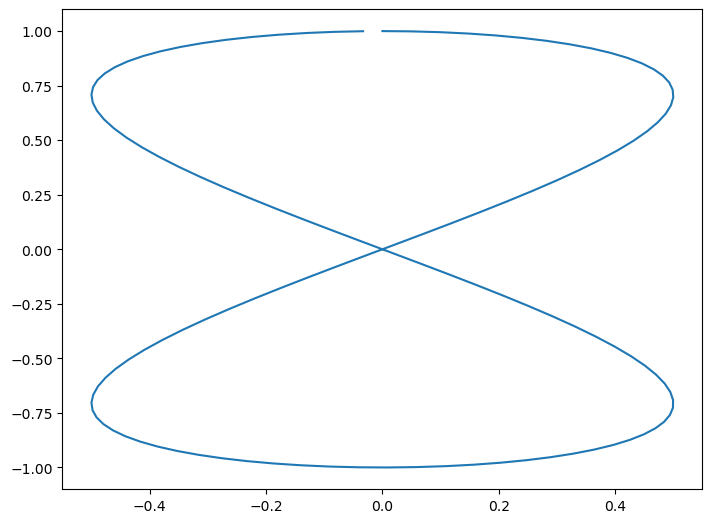
\includegraphics{chapters/python/00_prelims_files/figure-pdf/cell-2-output-1.png}

Quando lavori con il notebook, puoi essere all'interno di una cella,
digitando i suoi contenuti, oppure al di fuori delle celle, muovendoti
nel notebook.

Quando sei all'interno di una cella, premi Esc per uscirne. Quando ti
muovi al di fuori delle celle, premi Invio per entrare.

\begin{itemize}
\tightlist
\item
  Fuori da una cella:

  \begin{itemize}
  \tightlist
  \item
    Usa i tasti freccia per muoverti.
  \item
    Premi Shift+Invio per eseguire il codice nel blocco.
  \end{itemize}
\item
  All'interno di una cella:

  \begin{itemize}
  \tightlist
  \item
    Premi Tab per suggerire completamenti delle variabili.
  \end{itemize}
\end{itemize}

\begin{tcolorbox}[enhanced jigsaw, opacityback=0, breakable, left=2mm, opacitybacktitle=0.6, coltitle=black, rightrule=.15mm, colbacktitle=quarto-callout-note-color!10!white, colframe=quarto-callout-note-color-frame, toprule=.15mm, bottomtitle=1mm, toptitle=1mm, leftrule=.75mm, titlerule=0mm, title=\textcolor{quarto-callout-note-color}{\faInfo}\hspace{0.5em}{Nota}, arc=.35mm, bottomrule=.15mm, colback=white]

Il nome ``Jupyter'' deriva dalle tre principali lingue di programmazione
supportate: Julia, Python e R. Tuttavia, è possibile utilizzare i
Jupyter Notebook con molte altre lingue di programmazione.

\end{tcolorbox}

\section{Esecuzione Locale o su
Colab}\label{esecuzione-locale-o-su-colab}

I Jupyter Notebook possono essere eseguiti sia in locale, sul vostro
computer, che su un server remoto, come Google Colab. Questa
flessibilità permette agli utenti di accedere ai propri notebook da
qualsiasi dispositivo connesso a Internet e di condividere agevolmente
il proprio lavoro con altri.

\section{Kernel nei Jupyter Notebook}\label{kernel-nei-jupyter-notebook}

I Jupyter Notebook sono strumenti che agevolano la programmazione in
Python grazie a un componente essenziale: il kernel. Quest'ultimo funge
da motore di esecuzione per il codice Python presente nelle celle dei
notebook. Ogni volta che eseguite una cella, il suo contenuto viene
processato dal kernel. La caratteristica più significativa del kernel è
la sua capacità di preservare lo stato delle variabili e delle funzioni
tra le diverse celle. In pratica, ciò significa che potete definire
variabili o funzioni in una cella e poi riutilizzarle in celle
successive. Questa interattività facilita l'esecuzione iterativa del
codice e offre un modo dinamico per esplorare i dati.

Durante l'installazione di Jupyter Notebook, di norma ricevete anche
IPython, un kernel ottimizzato per Python.

Si noti che il kernel Python deve essere installato all'interno di un
ambiente di sviluppo dedicato noto come ``ambiente virtuale'' (per
ulteriori dettagli, si veda \{ref\}\texttt{sec-virtual-environment}).
Questo ambiente svolge un ruolo fondamentale nel separare e isolare le
librerie e le dipendenze necessarie per il kernel. Ciò aiuta a evitare
conflitti tra diverse configurazioni e garantisce il corretto
funzionamento del codice nel contesto desiderato. L'utilizzo di ambienti
specifici risulta particolarmente vantaggioso nei progetti che
richiedono versioni particolari di librerie.

In questo insegnamento, faremo ampio uso della funzionalità
\texttt{conda}, inclusa nell'installazione di Anaconda, per la gestione
di questi ambienti. \texttt{conda} mette a disposizione funzioni utili
per la creazione, la gestione e l'attivazione di ambienti separati,
ciascuno con le sue configurazioni e dipendenze uniche. Questa capacità
semplifica notevolmente la transizione tra diversi ambienti, garantendo
che ogni progetto o kernel disponga delle risorse necessarie per operare
in modo efficiente e senza interferenze.

\section{Visual Studio Code}\label{visual-studio-code}

Il modo più semplice di usare un Jupyter Notebook è all'interno di
Visual Studio Code. Dopo aver installato Visual Studio Code, è
necessario installare l'estensione Python per sfruttare le funzionalità
specifiche per Python, inclusa la capacità di lavorare con Jupyter
Notebook.

\begin{itemize}
\tightlist
\item
  In Visual Studio Code, si clicca sull'icona delle estensioni (quadrati
  che si intersecano) nella barra laterale a sinistra.
\item
  Si cerca ``Python'' nella barra di ricerca e si seleziona l'estensione
  ufficiale offerta da Microsoft.
\item
  Si clicca su ``Install''.
\end{itemize}

Una volta completate le installazioni, siete pronti per creare il vostro
primo Jupyter Notebook in VS Code.

\begin{itemize}
\tightlist
\item
  Si apre Visual Studio Code.
\item
  Si clicca su \texttt{File\ \textgreater{}\ New\ File}.
\item
  Si preme \texttt{Ctrl+Shift+P} per aprire la Palette dei Comandi.
\item
  Si digita ``Jupyter'' e si seleziona
  \texttt{Jupyter:\ Create\ New\ Blank\ Notebook}.
\item
  Si aprirà un nuovo notebook dove si può iniziare a scrivere il codice
  Python nelle celle.
\end{itemize}

\chapter{Python (1)}\label{sec-python-1}

\section{Scrivere Codice con il Supporto dei
LLM}\label{scrivere-codice-con-il-supporto-dei-llm}

I \emph{Large Language Models} (LLM), come GPT-4 o Claude, stanno
rivoluzionando non solo la generazione di testo in linguaggio naturale,
ma anche il campo della programmazione e dell'analisi dei dati. La
programmazione, con le sue regole esplicite e la sintassi strutturata,
si adatta particolarmente bene alle capacità di riconoscimento dei
pattern degli LLM. A differenza dei linguaggi umani, ricchi di ambiguità
ed espressioni idiomatiche, i linguaggi di programmazione sono rigorosi
e precisi.

Nel contesto dell'analisi dei dati, è naturale combinare le capacità
degli LLM con la potenza computazionale di linguaggi statistici come R o
di programmazione come Python. Sono già stati pubblicati libri su come
integrare le capacità degli LLM con l'analisi dei dati (Matter 2025), e
sta emergendo una nuova branca dell'ingegneria dedicata allo sviluppo
dei prompt più efficaci per l'uso con gli LLM. Pertanto, il problema non
è se utilizzare gli LLM a supporto della programmazione, ma come farlo
nel modo più efficace.

Gli LLM possono essere utilizzati per risolvere vari problemi di
programmazione in Python o R, basandosi su richieste formulate in
linguaggio naturale. Questi modelli sono in grado di generare codice,
identificare errori negli script, ottimizzare il codice, generare
documentazione e creare casi di test, anche per problemi di
programmazione complessi. L'avvento degli LLM ha cambiato radicalmente
il modo in cui sia i principianti sia i professionisti si approcciano
alla programmazione. Tuttavia, ciò non significa che gli LLM abbiano
completamente sostituito la scrittura di codice da parte degli esseri
umani. Piuttosto, gli LLM sono strumenti che possono migliorare
notevolmente il lavoro di chi ha già una buona conoscenza delle regole
sintattiche e dei principi di programmazione.

Un principio fondamentale da tenere a mente è che maggiore è la
conoscenza delle regole sintattiche di un linguaggio di programmazione,
maggiore sarà l'efficacia dell'uso degli LLM per scopi di analisi dei
dati. Anche se i problemi di programmazione trattati in questo corso
sono relativamente semplici rispetto alle capacità degli LLM, gli utenti
che sfrutteranno questi strumenti trarranno sicuramente vantaggio dalla
comprensione delle regole sintattiche del linguaggio di programmazione
utilizzato, principalmente Python (con alcuni esempi anche in R).

Gli LLM si basano sul concetto di ``predizione del prossimo token''.
Questo significa che sono addestrati per prevedere la parola o il
carattere successivo in una sequenza, basandosi sui precedenti. Questo
principio è alla base della capacità degli LLM di generare codice e di
migliorare i flussi di lavoro di analisi dei dati in Python o R. Oltre a
miliardi di parole provenienti da testi comuni (siti web, libri,
articoli di riviste), gli LLM di OpenAI, come GPT-4, sono stati
addestrati su un vasto corpus di codice open-source e discussioni sul
codice presenti su piattaforme come Stack Overflow. Questo consente loro
di generare codice sintatticamente e semanticamente corretto in molte
situazioni.

Nel mercato del lavoro attuale, acquisire competenze sull'uso pratico
dell'AI/LLM nella programmazione e nell'analisi dei dati è più di una
tendenza: è una necessità. I professionisti che sanno utilizzare
efficacemente l'AI/LLM per migliorare le loro competenze di
programmazione e integrare questi strumenti in Python e R avranno un
vantaggio competitivo. Con la crescente diffusione dell'AI e degli LLM
nell'industria e nel mondo accademico, la domanda per queste competenze
continuerà a crescere.

L'obiettivo di questo capitolo è fornire una panoramica della sintassi
di Python e delle principali funzioni di pacchetti come Pandas, Numpy e
Matplotlib, utili per la data science. Python è un linguaggio di
programmazione versatile e di facile lettura, adatto a numerosi usi.
Anche se il suo nome è un omaggio al gruppo comico
\href{https://www.youtube.com/results?search_query=monty+Python}{Monty
Python}, apprendere Python richiede tempo, pratica e impegno.

Questa guida (e l'intero corso) si concentra sull'insegnamento dei
principi fondamentali della programmazione, piuttosto che sui dettagli
tecnici. Facendo riferimento alla distinzione di Marr tra livello
computazionale e livello algoritmico (Marr 2010), una spiegazione a
livello computazionale descrive la logica del problema e i passaggi
necessari per trasformare l'input in output, mentre il livello
algoritmico specifica come eseguire queste operazioni logiche
utilizzando la sintassi di un particolare linguaggio di programmazione.

Il focus di questo corso è il livello computazionale, poiché è
fondamentale per comprendere i problemi e progettare soluzioni. Con
questa conoscenza, gli studenti saranno più capaci di risolvere problemi
specifici e di cercare autonomamente la sintassi appropriata per il
problema da risolvere.

Nell'era dell'intelligenza artificiale, è essenziale sviluppare la
capacità di pensare in modo computazionale. Questa competenza va oltre
la mera programmazione e offre un approccio strutturato per risolvere
problemi complessi. Sebbene i modelli di linguaggio avanzati (LLM) siano
in grado di risolvere molti dei problemi di programmazione affrontati in
questo corso, una comprensione approfondita dei principi della
programmazione rimane cruciale per interpretare, modificare o migliorare
le soluzioni proposte da tali sistemi.

In conclusione, anche nell'era dell'IA, una solida comprensione dei
fondamenti della programmazione è indispensabile per utilizzare
efficacemente gli strumenti avanzati come gli LLM e per navigare con
successo nel mondo della programmazione e dell'analisi dei dati.

\section{Espressioni e Operatori}\label{espressioni-e-operatori}

I programmi sono insiemi di espressioni che elaborano dati per fornire
istruzioni specifiche al computer. Ad esempio, in Python, l'operazione
di moltiplicazione si esegue utilizzando l'asterisco (\texttt{*}) tra
due numeri. Quando si incontra un'espressione come \texttt{3\ *\ 4}, il
computer la valuta e produce il risultato, che può essere visualizzato
in una cella successiva di un notebook Jupyter.

Le regole sintattiche in un linguaggio di programmazione come Python
sono stringenti. Ad esempio, non è consentito inserire due simboli
asterisco in sequenza senza un operando intermedio. Qualora
un'espressione violi queste norme sintattiche, il sistema ritornerà un
``SyntaxError'', un errore che indica la non conformità alle regole del
linguaggio. Per esempio

\begin{Shaded}
\begin{Highlighting}[]
\DecValTok{3} \OperatorTok{*} \OperatorTok{*} \DecValTok{4}
\end{Highlighting}
\end{Shaded}

restituisce:

\begin{Shaded}
\begin{Highlighting}[]
 \ExtensionTok{Cell}\NormalTok{ In}\PreprocessorTok{[}\SpecialStringTok{3}\PreprocessorTok{]}\NormalTok{, line 1}
    \ExtensionTok{3} \PreprocessorTok{*} \PreprocessorTok{*}\NormalTok{ 4}
        \ExtensionTok{\^{}}
\ExtensionTok{SyntaxError:}\NormalTok{ invalid syntax}
\end{Highlighting}
\end{Shaded}

Anche piccole modifiche in un'espressione possono cambiarne
completamente il significato. Nell'esempio successivo, lo spazio tra i
due asterischi \texttt{*} è stato rimosso. Tuttavia, poiché gli
asterischi compaiono tra due espressioni numeriche, l'espressione è
corretta e indica l'elevamento a potenza del primo numero al secondo: 3
elevato alla quarta potenza (\(3 \times 3 \times 3 \times 3\)). In
programmazione, simboli come \texttt{*} e \texttt{**} sono noti come
``operatori'', mentre i valori su cui agiscono sono denominati
``operandi''.

\begin{Shaded}
\begin{Highlighting}[]
\DecValTok{3} \OperatorTok{**} \DecValTok{4}
\end{Highlighting}
\end{Shaded}

\begin{verbatim}
81
\end{verbatim}

La tabella seguente elenca i principali operatori binari utilizzati in
Python, chiamati così perché agiscono su due operandi.

\begin{longtable}[]{@{}ll@{}}
\toprule\noalign{}
Operazione & Operatore \\
\midrule\noalign{}
\endhead
\bottomrule\noalign{}
\endlastfoot
addizione & \texttt{+} \\
sottrazione & \texttt{-} \\
moltiplicazione & \texttt{*} \\
divisione (reale) & \texttt{/} \\
divisione (intera; rimuove il resto) & \texttt{//} \\
resto (modulo) & \texttt{\%} \\
elevamento a potenza & \texttt{**} \\
\end{longtable}

Le due operazioni che potrebbero essere meno familiari sono \texttt{\%}
(trova il resto di una divisione) e \texttt{//} (esegui una divisione
scartando il resto).

Per esempio, la divisione intera (scartando il resto) di 11/2 produce 5.

\begin{Shaded}
\begin{Highlighting}[]
\DecValTok{11} \OperatorTok{//} \DecValTok{2}
\end{Highlighting}
\end{Shaded}

\begin{verbatim}
5
\end{verbatim}

Il resto di 11/2 è 1.

\begin{Shaded}
\begin{Highlighting}[]
\DecValTok{11} \OperatorTok{\%} \DecValTok{2}
\end{Highlighting}
\end{Shaded}

\begin{verbatim}
1
\end{verbatim}

Usando gli \textbf{operatori} che abbiamo elencato in precedenza
possiamo usare Python come un calcolatore.

\begin{Shaded}
\begin{Highlighting}[]
\BuiltInTok{print}\NormalTok{(}\StringTok{"4 + 2 è"}\NormalTok{, }\DecValTok{4} \OperatorTok{+} \DecValTok{2}\NormalTok{)}
\BuiltInTok{print}\NormalTok{(}\StringTok{"4 {-} 2 è"}\NormalTok{, }\DecValTok{4} \OperatorTok{{-}} \DecValTok{2}\NormalTok{)}
\BuiltInTok{print}\NormalTok{(}\StringTok{"4 * 2 è"}\NormalTok{, }\DecValTok{4} \OperatorTok{*} \DecValTok{2}\NormalTok{)}
\BuiltInTok{print}\NormalTok{(}\StringTok{"4 / 2 è"}\NormalTok{, }\DecValTok{4} \OperatorTok{/} \DecValTok{2}\NormalTok{)}
\BuiltInTok{print}\NormalTok{(}\StringTok{"4 ** 2 è"}\NormalTok{, }\DecValTok{4}\OperatorTok{**}\DecValTok{2}\NormalTok{)}
\BuiltInTok{print}\NormalTok{(}\StringTok{"9 \% 4 è"}\NormalTok{, }\DecValTok{9} \OperatorTok{\%} \DecValTok{4}\NormalTok{)}
\BuiltInTok{print}\NormalTok{(}\StringTok{"9 // 4 è"}\NormalTok{, }\DecValTok{9} \OperatorTok{//} \DecValTok{4}\NormalTok{)}
\end{Highlighting}
\end{Shaded}

\begin{verbatim}
4 + 2 è 6
4 - 2 è 2
4 * 2 è 8
4 / 2 è 2.0
4 ** 2 è 16
9 % 4 è 1
9 // 4 è 2
\end{verbatim}

L'applicazione degli operatori aritmetici in Python dipende dalle
seguenti regole di precedenza degli operatori, che sono analoghe a
quelle usate in algebra.

\begin{enumerate}
\def\labelenumi{\arabic{enumi}.}
\tightlist
\item
  Le espressioni tra parentesi vengono valutate per prime.
\item
  Successivamente si valutano gli elevamenti a potenza.
\item
  In seguito, si valutano moltiplicazioni, divisioni e moduli.
\item
  Per ultime vengono valutate somme e sottrazioni.
\end{enumerate}

\begin{Shaded}
\begin{Highlighting}[]
\DecValTok{1} \OperatorTok{+} \DecValTok{2} \OperatorTok{*} \DecValTok{3} \OperatorTok{*} \DecValTok{4} \OperatorTok{*} \DecValTok{5} \OperatorTok{/} \DecValTok{6} \OperatorTok{**} \DecValTok{3} \OperatorTok{+} \DecValTok{7} \OperatorTok{+} \DecValTok{8} \OperatorTok{{-}} \DecValTok{9} \OperatorTok{+} \DecValTok{10}
\end{Highlighting}
\end{Shaded}

\begin{verbatim}
17.555555555555557
\end{verbatim}

\begin{Shaded}
\begin{Highlighting}[]
\DecValTok{1} \OperatorTok{+} \DecValTok{2} \OperatorTok{*}\NormalTok{ (}\DecValTok{3} \OperatorTok{*} \DecValTok{4} \OperatorTok{*} \DecValTok{5} \OperatorTok{/} \DecValTok{6}\NormalTok{) }\OperatorTok{**} \DecValTok{3} \OperatorTok{+} \DecValTok{7} \OperatorTok{+} \DecValTok{8} \OperatorTok{{-}} \DecValTok{9} \OperatorTok{+} \DecValTok{10}
\end{Highlighting}
\end{Shaded}

\begin{verbatim}
2017.0
\end{verbatim}

\section{Variabili}\label{variabili}

Quando generiamo un risultato, la risposta viene visualizzata ma non
viene memorizzata da nessuna parte, come abbiamo visto negli esempi
precedenti. Se vogliamo recuperare quel risultato, dobbiamo
memorizzarlo. Lo mettiamo in un oggetto, e diamo un nome a
quell'oggetto. Questa è una variabile.

Per creare una variabile facciamo uso di un'istruzione di assegnazione.
In un'istruzione di assegnazione, si specifica un nome seguito dal
simbolo di uguale (=) e dall'espressione che si desidera assegnare a
tale nome. L'operazione di assegnazione consiste nell'associare il
valore dell'espressione a destra del simbolo di uguale al nome a
sinistra. Da quel momento in poi, ogni volta che il nome viene
utilizzato in un'espressione, il valore associato durante l'assegnazione
viene utilizzato al suo posto.

\begin{Shaded}
\begin{Highlighting}[]
\NormalTok{a }\OperatorTok{=} \DecValTok{10}
\NormalTok{b }\OperatorTok{=} \DecValTok{20}
\NormalTok{a }\OperatorTok{+}\NormalTok{ b}
\end{Highlighting}
\end{Shaded}

\begin{verbatim}
30
\end{verbatim}

\begin{Shaded}
\begin{Highlighting}[]
\NormalTok{a }\OperatorTok{=} \DecValTok{1}\OperatorTok{/}\DecValTok{4}
\NormalTok{b }\OperatorTok{=} \DecValTok{2} \OperatorTok{*}\NormalTok{ a}
\NormalTok{b}
\end{Highlighting}
\end{Shaded}

\begin{verbatim}
0.5
\end{verbatim}

\begin{Shaded}
\begin{Highlighting}[]
\NormalTok{my\_var }\OperatorTok{=} \DecValTok{100}
\NormalTok{const }\OperatorTok{=} \DecValTok{3}

\NormalTok{my\_var }\OperatorTok{*}\NormalTok{ const}
\end{Highlighting}
\end{Shaded}

\begin{verbatim}
300
\end{verbatim}

In Python, ogni ``oggetto'' è un'area di memoria nel computer. Una
``variabile'' funge da etichetta che fa riferimento a quest'area. Se un
oggetto non ha più etichette (ovvero, non ci sono più variabili che lo
referenziano), i dati contenuti nell'oggetto diventano inaccessibili. Il
Garbage Collector del linguaggio si occuperà di rilevare questi oggetti
non referenziati e liberare la memoria, permettendo che venga
riutilizzata per nuovi dati.

\section{Nomi delle Variabili}\label{nomi-delle-variabili}

I nomi delle variabili in Python possono contenere caratteri
alfanumerici da a-z, A-Z, 0-9 e alcuni caratteri speciali come \_. I
nomi delle variabili normali devono iniziare con una lettera. I nomi
delle variabili non possono contenere uno spazio; invece, è comune
utilizzare il carattere \texttt{\_} per sostituire ogni spazio. Sta al
programmatore scegliere nomi facili da interpretare.

Per convenzione, i nomi delle variabili iniziano con una lettera
minuscola, mentre i nomi delle classi iniziano con una lettera
maiuscola.

Inoltre, ci sono una serie di parole chiave (\emph{keyword}) in Python
che non possono essere utilizzate come nomi di variabili. Queste parole
chiave sono:

\begin{Shaded}
\begin{Highlighting}[]
\ImportTok{import}\NormalTok{ keyword}
\BuiltInTok{print}\NormalTok{(}\OperatorTok{*}\NormalTok{keyword.kwlist, sep}\OperatorTok{=}\StringTok{"}\CharTok{\textbackslash{}n}\StringTok{"}\NormalTok{)}
\end{Highlighting}
\end{Shaded}

\begin{verbatim}
False
None
True
and
as
assert
async
await
break
class
continue
def
del
elif
else
except
finally
for
from
global
if
import
in
is
lambda
nonlocal
not
or
pass
raise
return
try
while
with
yield
\end{verbatim}

Si presti attenzione alla parola chiave ``lambda'', che potrebbe
facilmente essere un nome di variabile naturale in un programma
scientifico. Tuttavia, essendo una parola chiave, non può essere
utilizzata come nome di variabile.

\section{Tipologie di Dati in Python}\label{tipologie-di-dati-in-python}

In Python, le variabili possono appartenere a diverse tipologie di dati,
ciascuna con caratteristiche e utilizzi specifici.

\subsection{Stringhe (String)}\label{stringhe-string}

Le stringhe sono sequenze di caratteri, utilizzate per rappresentare
testo. In Python, le stringhe possono essere create utilizzando apici
singoli (\texttt{\textquotesingle{}\ \textquotesingle{}}), doppi
(\texttt{"\ "}) o tripli
(\texttt{\textquotesingle{}\textquotesingle{}\textquotesingle{}\ \textquotesingle{}\textquotesingle{}\textquotesingle{}}
oppure \texttt{"""\ """}) per delimitare il testo. Esempi di stringhe
sono:

\begin{verbatim}
"Hello, world!"
'Beyonce-Lemonade.txt'
"lemonade"
\end{verbatim}

Si noti il risultato ottenuto quando si applica l'operatore \texttt{+} a
due stringhe.

\begin{Shaded}
\begin{Highlighting}[]
\CommentTok{"data"} \OperatorTok{+} \StringTok{"science"}
\end{Highlighting}
\end{Shaded}

\begin{verbatim}
'datascience'
\end{verbatim}

\begin{Shaded}
\begin{Highlighting}[]
\CommentTok{"data"} \OperatorTok{+} \StringTok{" "} \OperatorTok{+} \StringTok{"science"}
\end{Highlighting}
\end{Shaded}

\begin{verbatim}
'data science'
\end{verbatim}

Sia le virgolette singole che doppie possono essere utilizzate per
creare le stringhe: ``ciao'' e `ciao' sono espressioni equivalenti.
Tuttavia, le virgolette doppie sono spesso preferite poiché consentono
di includere virgolette singole all'interno delle stringhe.

\begin{Shaded}
\begin{Highlighting}[]
\CommentTok{"Che cos\textquotesingle{}è una parola?"}
\end{Highlighting}
\end{Shaded}

\begin{verbatim}
"Che cos'è una parola?"
\end{verbatim}

L'espressione precedente avrebbe prodotto un \texttt{SyntaxError} se
fosse stata racchiusa da virgolette singole.

\subsubsection{Parsing strings}\label{parsing-strings}

In Python, una stringa è concepita come una sequenza ordinata di
caratteri. Grazie all'operatore di indicizzazione, rappresentato dalle
parentesi quadre \texttt{{[}{]}}, è possibile accedere a singoli
elementi della stringa.

È importante ricordare che l'indicizzazione in Python parte da zero.

L'indice del primo carattere è \texttt{{[}0{]}}, quello del secondo è
\texttt{{[}1{]}}, del terzo \texttt{{[}2{]}}, e così via. Questa
funzionalità consente di manipolare o consultare specifici segmenti
della stringa, piuttosto che gestirla come un blocco unico.

Consideriamo questo verso di Eugenio Montale:

\begin{Shaded}
\begin{Highlighting}[]
\NormalTok{my\_string }\OperatorTok{=} \StringTok{"Tendono alla chiarità le cose oscure"}
\BuiltInTok{print}\NormalTok{(my\_string)}
\end{Highlighting}
\end{Shaded}

\begin{verbatim}
Tendono alla chiarità le cose oscure
\end{verbatim}

\begin{Shaded}
\begin{Highlighting}[]
\NormalTok{my\_string[}\DecValTok{0}\NormalTok{]}
\end{Highlighting}
\end{Shaded}

\begin{verbatim}
'T'
\end{verbatim}

\begin{Shaded}
\begin{Highlighting}[]
\NormalTok{my\_string[}\DecValTok{3}\NormalTok{]}
\end{Highlighting}
\end{Shaded}

\begin{verbatim}
'd'
\end{verbatim}

\begin{Shaded}
\begin{Highlighting}[]
\BuiltInTok{len}\NormalTok{(my\_string)}
\end{Highlighting}
\end{Shaded}

\begin{verbatim}
36
\end{verbatim}

La stringa ``my\_string'' conta 36 caratteri. Pertanto, gli indici
validi per questa stringa vanno da 0 a 35. Per accedere all'ultimo
carattere, è necessario utilizzare l'indice 35, che corrisponde a 36
meno 1.

\begin{Shaded}
\begin{Highlighting}[]
\NormalTok{my\_string[}\DecValTok{35}\NormalTok{]}
\end{Highlighting}
\end{Shaded}

\begin{verbatim}
'e'
\end{verbatim}

Un modo efficiente per ottenere l'ultimo carattere è ricorrere alla
funzione \texttt{len}, sottraendo 1 al risultato:

\begin{Shaded}
\begin{Highlighting}[]
\NormalTok{my\_string[}\BuiltInTok{len}\NormalTok{(my\_string) }\OperatorTok{{-}} \DecValTok{1}\NormalTok{]}
\end{Highlighting}
\end{Shaded}

\begin{verbatim}
'e'
\end{verbatim}

Si noti che \texttt{len()} è una funzione. Una funzione è un blocco di
codice che esegue un'operazione specifica. I programmatori chiamano
anche gli input delle funzioni ``parametri'' o ``argomenti''.

La funzione \texttt{len} prende un input e restituisce un output.
L'output è la lunghezza di ciò che è stato passato come input.

\subsubsection{Slicing strings}\label{slicing-strings}

Oltre a estrarre caratteri individuali da una stringa, Python offre la
possibilità di selezionare segmenti di testo attraverso la tecnica dello
``slicing''. Questo meccanismo è simile all'indicizzazione, ma utilizza
due indici separati da un carattere a due punti (:). Il primo indice
indica la posizione di partenza dello ``slicing'' nella stringa, mentre
il secondo indice segnala il punto in cui terminare l'estrazione del
segmento.

\begin{Shaded}
\begin{Highlighting}[]
\NormalTok{my\_string[}\DecValTok{2}\NormalTok{:}\DecValTok{4}\NormalTok{]}
\end{Highlighting}
\end{Shaded}

\begin{verbatim}
'nd'
\end{verbatim}

Se si omette il primo indice, Python utilizzerà l'inizio della stringa;
se si omette il secondo, utilizzerà la fine della stringa.

\begin{Shaded}
\begin{Highlighting}[]
\NormalTok{my\_string[:}\DecValTok{4}\NormalTok{]}
\end{Highlighting}
\end{Shaded}

\begin{verbatim}
'Tend'
\end{verbatim}

\begin{Shaded}
\begin{Highlighting}[]
\NormalTok{my\_string[}\DecValTok{4}\NormalTok{:]}
\end{Highlighting}
\end{Shaded}

\begin{verbatim}
'ono alla chiarità le cose oscure'
\end{verbatim}

\subsubsection{Metodi}\label{metodi}

A partire da una stringa esistente, si possono generare nuove stringhe
mediante l'utilizzo di \emph{metodi} specifici per le stringhe. Questi
metodi sono essenzialmente funzioni che agiscono direttamente
sull'oggetto stringa. Per invocare un metodo, basta posizionare un punto
subito dopo la stringa e seguire con il nome del metodo desiderato. Ad
esempio, il metodo successivo converte tutti i caratteri della stringa
in maiuscole.

\begin{Shaded}
\begin{Highlighting}[]
\NormalTok{my\_string.upper()}
\end{Highlighting}
\end{Shaded}

\begin{verbatim}
'TENDONO ALLA CHIARITÀ LE COSE OSCURE'
\end{verbatim}

Il metodo \texttt{my\_string.title()} è utilizzato per convertire la
prima lettera di ogni parola nella stringa \texttt{my\_string} in
maiuscolo, mentre rende tutte le altre lettere minuscole. In pratica,
trasforma la stringa in una forma ``a titolo'', in cui ogni parola
inizia con una lettera maiuscola.

\begin{Shaded}
\begin{Highlighting}[]
\NormalTok{my\_string.title()}
\end{Highlighting}
\end{Shaded}

\begin{verbatim}
'Tendono Alla Chiarità Le Cose Oscure'
\end{verbatim}

\subsection{Numeri Interi (Integer)}\label{numeri-interi-integer}

I numeri interi rappresentano numeri senza una componente decimale. In
Python, possono essere creati assegnando un valore senza parte decimale
a una variabile. Esempio di un numero intero è:

\begin{Shaded}
\begin{Highlighting}[]
\NormalTok{age }\OperatorTok{=} \DecValTok{20}
\end{Highlighting}
\end{Shaded}

\subsection{Numeri in Virgola Mobile
(Float)}\label{numeri-in-virgola-mobile-float}

I numeri in virgola mobile, o ``float'', rappresentano numeri che hanno
una componente decimale. Sono creati assegnando un valore con una parte
decimale a una variabile. Esempio di un numero float è:

\begin{Shaded}
\begin{Highlighting}[]
\NormalTok{temperature }\OperatorTok{=} \FloatTok{36.4}
\end{Highlighting}
\end{Shaded}

I numeri in virgola mobile, o ``float'', hanno una precisione limitata a
circa 15-16 cifre decimali; oltre questo limite, la precisione viene
persa. Nonostante questa limitazione, sono sufficienti per la maggior
parte delle applicazioni.

Inoltre, è possibile utilizzare la notazione scientifica per
rappresentare numeri molto grandi o molto piccoli. In questa notazione,
\texttt{m\ *\ 10\^{}n} viene comunemente abbreviato come \texttt{mEn},
dove ``E'' rappresenta l'esponente dieci. Ad esempio, \texttt{1E9}
equivale a un miliardo (\(1 \times 10^9\)) e \texttt{1E-9} rappresenta
un miliardesimo (\(1 \times 10^{-9}\)).

\subsection{Valori Booleani (Boolean)}\label{valori-booleani-boolean}

I valori booleani possono assumere solo due stati: vero (\texttt{True})
o falso (\texttt{False}). Sono utilizzati per rappresentare le
condizioni logiche e sono ottenuti attraverso espressioni di confronto.
Esempio di un valore booleano è:

\begin{Shaded}
\begin{Highlighting}[]
\NormalTok{is\_raining }\OperatorTok{=} \VariableTok{False}
\end{Highlighting}
\end{Shaded}

Nel contesto delle operazioni aritmetiche, \texttt{True} è equivalente
al numero intero 1, mentre \texttt{False} corrisponde a 0. Questo
permette di includere valori booleani in calcoli matematici. Per
esempio:

\begin{Shaded}
\begin{Highlighting}[]
\VariableTok{True} \OperatorTok{+} \VariableTok{True} \OperatorTok{+} \VariableTok{False}
\end{Highlighting}
\end{Shaded}

\begin{verbatim}
2
\end{verbatim}

Un valore booleano viene ritornato quando si valuta un confronto. Per
esempio:

\begin{Shaded}
\begin{Highlighting}[]
\DecValTok{3} \OperatorTok{\textgreater{}} \DecValTok{1} \OperatorTok{+} \DecValTok{1}
\end{Highlighting}
\end{Shaded}

Il valore True indica che il confronto è valido; Python ha confermato
questo semplice fatto sulla relazione tra 3 e 1+1.

Si noti la regola di precedenza: gli operatori \textgreater, \textless,
\textgreater=, \textless=, ==, != hanno la precedenza più bassa (vengono
valutati per ultimi), il che significa che nell'espressione precedente
viene prima valutato (1 + 1) e poi (3 \textgreater{} 2).

\subsection{Operatori di confronto}\label{operatori-di-confronto}

Un operatore di confronto è un operatore che esegue un qualche tipo di
confronto e restituisce un valore booleano (True oppure False). Per
esempio, l'operatore \texttt{==} confronta le espressioni su entrambi i
lati e restituisce \texttt{True} se hanno gli stessi valori e
\texttt{False} altrimenti. L'opposto di \texttt{==} è \texttt{!=}, che
si può leggere come `non uguale al valore di'. Gli operatori di
confronto sono elencati qui sotto:

\begin{longtable}[]{@{}ll@{}}
\toprule\noalign{}
Confronto & Operatore \\
\midrule\noalign{}
\endhead
\bottomrule\noalign{}
\endlastfoot
Minore & \textless{} \\
Maggiore & \textgreater{} \\
Minore o uguale & \textless= \\
Maggiore o uguale & \textgreater= \\
Uguale & == \\
Non uguale & != \\
\end{longtable}

Ad esempio:

\begin{Shaded}
\begin{Highlighting}[]
\NormalTok{a }\OperatorTok{=} \DecValTok{4}
\NormalTok{b }\OperatorTok{=} \DecValTok{2}

\BuiltInTok{print}\NormalTok{(}\StringTok{"a \textgreater{} b"}\NormalTok{, }\StringTok{"is"}\NormalTok{, a }\OperatorTok{\textgreater{}}\NormalTok{ b)}
\BuiltInTok{print}\NormalTok{(}\StringTok{"a \textless{} b"}\NormalTok{, }\StringTok{"is"}\NormalTok{, a }\OperatorTok{\textless{}}\NormalTok{ b)}
\BuiltInTok{print}\NormalTok{(}\StringTok{"a == b"}\NormalTok{, }\StringTok{"is"}\NormalTok{, a }\OperatorTok{==}\NormalTok{ b)}
\BuiltInTok{print}\NormalTok{(}\StringTok{"a \textgreater{}= b"}\NormalTok{, }\StringTok{"is"}\NormalTok{, a }\OperatorTok{\textgreater{}=}\NormalTok{ b)}
\BuiltInTok{print}\NormalTok{(}\StringTok{"a \textless{}= b"}\NormalTok{, }\StringTok{"is"}\NormalTok{, a }\OperatorTok{\textless{}=}\NormalTok{ b)}
\end{Highlighting}
\end{Shaded}

Nella cella seguente si presti attenzione all'uso di \texttt{=} e di
\texttt{==}:

\begin{Shaded}
\begin{Highlighting}[]
\NormalTok{boolean\_condition }\OperatorTok{=} \DecValTok{10} \OperatorTok{==} \DecValTok{20}
\BuiltInTok{print}\NormalTok{(boolean\_condition)}
\end{Highlighting}
\end{Shaded}

L'operatore \texttt{=} è un'istruzione di \emph{assegnazione}. Ovvero,
crea un nuovo oggetto. L'operatore \texttt{==} valuta invece una
condizione logica e ritorna un valore booleano.

Un'espressione può contenere più confronti e tutti devono essere veri
affinché l'intera espressione sia vera. Ad esempio:

\begin{Shaded}
\begin{Highlighting}[]
\DecValTok{1} \OperatorTok{\textless{}} \DecValTok{1} \OperatorTok{+} \DecValTok{1} \OperatorTok{\textless{}} \DecValTok{3}
\end{Highlighting}
\end{Shaded}

\subsection{Tipizzazione Dinamica in
Python}\label{tipizzazione-dinamica-in-python}

Python è un linguaggio con tipizzazione dinamica, il che significa che
il tipo di una variabile è determinato dal valore che le viene assegnato
durante l'esecuzione del programma e non necessita di essere dichiarato
esplicitamente.

Per identificare il tipo di una variabile o del risultato di
un'espressione, Python mette a disposizione la funzione \texttt{type()}.
Questa funzione, quando chiamata con una variabile o un'espressione come
argomento, restituisce il tipo di dati corrispondente.

Nell'esempio seguente il programma stamperà
\texttt{\textless{}class\ \textquotesingle{}str\textquotesingle{}\textgreater{}},
indicando che \texttt{x} è una variabile di tipo ``stringa''.

\begin{Shaded}
\begin{Highlighting}[]
\NormalTok{x }\OperatorTok{=} \StringTok{"hello"}
\BuiltInTok{print}\NormalTok{(}\BuiltInTok{type}\NormalTok{(x))}
\end{Highlighting}
\end{Shaded}

\begin{verbatim}
<class 'str'>
\end{verbatim}

Applichiamo la funzione \texttt{type()} alle altre variabili che abbiamo
definito in precedenza.

\begin{Shaded}
\begin{Highlighting}[]
\NormalTok{age }\OperatorTok{=} \DecValTok{20}
\BuiltInTok{print}\NormalTok{(}\BuiltInTok{type}\NormalTok{(age))}
\end{Highlighting}
\end{Shaded}

\begin{verbatim}
<class 'int'>
\end{verbatim}

\begin{Shaded}
\begin{Highlighting}[]
\NormalTok{temperature }\OperatorTok{=} \FloatTok{36.4}
\BuiltInTok{print}\NormalTok{(}\BuiltInTok{type}\NormalTok{(temperature))}
\end{Highlighting}
\end{Shaded}

\begin{verbatim}
<class 'float'>
\end{verbatim}

\begin{Shaded}
\begin{Highlighting}[]
\NormalTok{is\_raining }\OperatorTok{=} \VariableTok{False}
\BuiltInTok{print}\NormalTok{(}\BuiltInTok{type}\NormalTok{(is\_raining))}
\end{Highlighting}
\end{Shaded}

\begin{verbatim}
<class 'bool'>
\end{verbatim}

\subsection{Operatori Booleani}\label{operatori-booleani}

Gli operatori booleani (o operatori logici) confrontano
\emph{espressioni} (non valori) e ritornano un valore booleano. Python
ha tre operatori logici:

\begin{itemize}
\tightlist
\item
  \texttt{and} -- Ritorna True solo se entrambi le espressioni sono
  vere, altrimenti ritorna False
\item
  \texttt{or} -- Ritorna True se almeno una delle due espressioni è
  vera, altrimenti ritorna False.
\item
  \texttt{not} -- Ritorna True se l'espressione è falsa, altrimenti
  ritorna False.
\end{itemize}

Ad esempio:

\begin{Shaded}
\begin{Highlighting}[]
\NormalTok{a }\OperatorTok{=} \DecValTok{2}
\NormalTok{b }\OperatorTok{=} \DecValTok{3}

\NormalTok{(a }\OperatorTok{+}\NormalTok{ b }\OperatorTok{\textgreater{}}\NormalTok{ a) }\KeywordTok{and}\NormalTok{ (a }\OperatorTok{+}\NormalTok{ b }\OperatorTok{\textgreater{}}\NormalTok{ b)}
\end{Highlighting}
\end{Shaded}

\begin{verbatim}
True
\end{verbatim}

Nella cella sopra le parentesi tonde sono opzionali ma facilitano la
lettura.

L'operatore \texttt{and} restituisce \texttt{True} solo se entrambe le
condizioni booleane sono vere. Ad esempio, \texttt{True\ and\ False}
restituirà \texttt{False} perché una delle condizioni è falsa:

\begin{Shaded}
\begin{Highlighting}[]
\VariableTok{True} \KeywordTok{and} \VariableTok{False}
\end{Highlighting}
\end{Shaded}

\begin{verbatim}
False
\end{verbatim}

L'operatore \texttt{or} restituisce \texttt{True} se almeno una delle
due condizioni booleane è vera. Ad esempio, \texttt{True\ or\ False}
restituirà \texttt{True} perché almeno una delle condizioni è vera.

\begin{Shaded}
\begin{Highlighting}[]
\VariableTok{True} \KeywordTok{or} \VariableTok{False}
\end{Highlighting}
\end{Shaded}

\begin{verbatim}
True
\end{verbatim}

L'operatore \texttt{not} viene utilizzato per invertire il valore di
verità di una condizione booleana. Ad esempio, \texttt{not\ True}
restituirà \texttt{False} e \texttt{not\ False} restituirà
\texttt{True}.

\begin{Shaded}
\begin{Highlighting}[]
\KeywordTok{not} \VariableTok{True}
\end{Highlighting}
\end{Shaded}

\begin{verbatim}
False
\end{verbatim}

Alcuni esempi sono i seguenti (si noti l'uso della funzione
\texttt{len()}):

\begin{Shaded}
\begin{Highlighting}[]
\BuiltInTok{print}\NormalTok{(}\DecValTok{3} \OperatorTok{\textgreater{}} \DecValTok{2}\NormalTok{)  }\CommentTok{\# True, because 3 is greater than 2}
\BuiltInTok{print}\NormalTok{(}\DecValTok{3} \OperatorTok{\textgreater{}=} \DecValTok{2}\NormalTok{)  }\CommentTok{\# True, because 3 is greater than 2}
\BuiltInTok{print}\NormalTok{(}\DecValTok{3} \OperatorTok{\textless{}} \DecValTok{2}\NormalTok{)  }\CommentTok{\# False,  because 3 is greater than 2}
\BuiltInTok{print}\NormalTok{(}\DecValTok{2} \OperatorTok{\textless{}} \DecValTok{3}\NormalTok{)  }\CommentTok{\# True, because 2 is less than 3}
\BuiltInTok{print}\NormalTok{(}\DecValTok{2} \OperatorTok{\textless{}=} \DecValTok{3}\NormalTok{)  }\CommentTok{\# True, because 2 is less than 3}
\BuiltInTok{print}\NormalTok{(}\DecValTok{3} \OperatorTok{==} \DecValTok{2}\NormalTok{)  }\CommentTok{\# False, because 3 is not equal to 2}
\BuiltInTok{print}\NormalTok{(}\DecValTok{3} \OperatorTok{!=} \DecValTok{2}\NormalTok{)  }\CommentTok{\# True, because 3 is not equal to 2}
\BuiltInTok{print}\NormalTok{(}\BuiltInTok{len}\NormalTok{(}\StringTok{"mango"}\NormalTok{) }\OperatorTok{==} \BuiltInTok{len}\NormalTok{(}\StringTok{"avocado"}\NormalTok{))  }\CommentTok{\# False}
\BuiltInTok{print}\NormalTok{(}\BuiltInTok{len}\NormalTok{(}\StringTok{"mango"}\NormalTok{) }\OperatorTok{!=} \BuiltInTok{len}\NormalTok{(}\StringTok{"avocado"}\NormalTok{))  }\CommentTok{\# True}
\BuiltInTok{print}\NormalTok{(}\BuiltInTok{len}\NormalTok{(}\StringTok{"mango"}\NormalTok{) }\OperatorTok{\textless{}} \BuiltInTok{len}\NormalTok{(}\StringTok{"avocado"}\NormalTok{))  }\CommentTok{\# True}
\BuiltInTok{print}\NormalTok{(}\BuiltInTok{len}\NormalTok{(}\StringTok{"milk"}\NormalTok{) }\OperatorTok{!=} \BuiltInTok{len}\NormalTok{(}\StringTok{"meat"}\NormalTok{))  }\CommentTok{\# False}
\BuiltInTok{print}\NormalTok{(}\BuiltInTok{len}\NormalTok{(}\StringTok{"milk"}\NormalTok{) }\OperatorTok{==} \BuiltInTok{len}\NormalTok{(}\StringTok{"meat"}\NormalTok{))  }\CommentTok{\# True}
\BuiltInTok{print}\NormalTok{(}\BuiltInTok{len}\NormalTok{(}\StringTok{"tomato"}\NormalTok{) }\OperatorTok{==} \BuiltInTok{len}\NormalTok{(}\StringTok{"potato"}\NormalTok{))  }\CommentTok{\# True}
\BuiltInTok{print}\NormalTok{(}\BuiltInTok{len}\NormalTok{(}\StringTok{"python"}\NormalTok{) }\OperatorTok{\textgreater{}} \BuiltInTok{len}\NormalTok{(}\StringTok{"dragon"}\NormalTok{))  }\CommentTok{\# False}
\end{Highlighting}
\end{Shaded}

\begin{verbatim}
True
True
False
True
True
False
True
False
True
True
False
True
True
False
\end{verbatim}

Altri esempi di come questi operatori possono essere utilizzati sono i
seguenti:

\begin{Shaded}
\begin{Highlighting}[]
\BuiltInTok{print}\NormalTok{(}\DecValTok{3} \OperatorTok{\textgreater{}} \DecValTok{2} \KeywordTok{and} \DecValTok{4} \OperatorTok{\textgreater{}} \DecValTok{3}\NormalTok{)  }\CommentTok{\# True {-} because both statements are true}
\BuiltInTok{print}\NormalTok{(}\DecValTok{3} \OperatorTok{\textgreater{}} \DecValTok{2} \KeywordTok{and} \DecValTok{4} \OperatorTok{\textless{}} \DecValTok{3}\NormalTok{)  }\CommentTok{\# False {-} because the second statement is false}
\BuiltInTok{print}\NormalTok{(}\DecValTok{3} \OperatorTok{\textless{}} \DecValTok{2} \KeywordTok{and} \DecValTok{4} \OperatorTok{\textless{}} \DecValTok{3}\NormalTok{)  }\CommentTok{\# False {-} because both statements are false}
\BuiltInTok{print}\NormalTok{(}\StringTok{"True and True: "}\NormalTok{, }\VariableTok{True} \KeywordTok{and} \VariableTok{True}\NormalTok{)}
\BuiltInTok{print}\NormalTok{(}\DecValTok{3} \OperatorTok{\textgreater{}} \DecValTok{2} \KeywordTok{or} \DecValTok{4} \OperatorTok{\textgreater{}} \DecValTok{3}\NormalTok{)  }\CommentTok{\# True {-} because both statements are true}
\BuiltInTok{print}\NormalTok{(}\DecValTok{3} \OperatorTok{\textgreater{}} \DecValTok{2} \KeywordTok{or} \DecValTok{4} \OperatorTok{\textless{}} \DecValTok{3}\NormalTok{)  }\CommentTok{\# True {-} because one of the statements is true}
\BuiltInTok{print}\NormalTok{(}\DecValTok{3} \OperatorTok{\textless{}} \DecValTok{2} \KeywordTok{or} \DecValTok{4} \OperatorTok{\textless{}} \DecValTok{3}\NormalTok{)  }\CommentTok{\# False {-} because both statements are false}
\BuiltInTok{print}\NormalTok{(}\StringTok{"True or False:"}\NormalTok{, }\VariableTok{True} \KeywordTok{or} \VariableTok{False}\NormalTok{)}
\BuiltInTok{print}\NormalTok{(}\KeywordTok{not} \DecValTok{3} \OperatorTok{\textgreater{}} \DecValTok{2}\NormalTok{)  }\CommentTok{\# False {-} because 3 \textgreater{} 2 is true, then not True gives False}
\BuiltInTok{print}\NormalTok{(}\KeywordTok{not} \VariableTok{True}\NormalTok{)  }\CommentTok{\# False {-} Negation, the not operator turns true to false}
\BuiltInTok{print}\NormalTok{(}\KeywordTok{not} \VariableTok{False}\NormalTok{)  }\CommentTok{\# True}
\BuiltInTok{print}\NormalTok{(}\KeywordTok{not} \KeywordTok{not} \VariableTok{True}\NormalTok{)  }\CommentTok{\# True}
\BuiltInTok{print}\NormalTok{(}\KeywordTok{not} \KeywordTok{not} \VariableTok{False}\NormalTok{)  }\CommentTok{\# False}
\end{Highlighting}
\end{Shaded}

\begin{verbatim}
True
False
False
True and True:  True
True
True
False
True or False: True
False
False
True
True
False
\end{verbatim}

Abbiamo tralasciato alcuni operatori in Python. Due di quelli che
abbiamo omesso sono gli operatori di appartenenza, \texttt{in} e
\texttt{not\ in}. Gli altri operatori che abbiamo tralasciato sono gli
operatori bitwise e gli operatori sugli insiemi, che verranno trattati
in seguito.

\subsection{Valori Numerici di True e
False}\label{valori-numerici-di-true-e-false}

È fondamentale comprendere i valori numerici associati alle parole
chiave \texttt{True} e \texttt{False}. Queste due parole chiave hanno i
valori numerici di 1 e 0, rispettivamente.

\begin{Shaded}
\begin{Highlighting}[]
\VariableTok{True} \OperatorTok{==} \DecValTok{1}
\end{Highlighting}
\end{Shaded}

\begin{verbatim}
True
\end{verbatim}

\begin{Shaded}
\begin{Highlighting}[]
\VariableTok{False} \OperatorTok{==} \DecValTok{0}
\end{Highlighting}
\end{Shaded}

\begin{verbatim}
True
\end{verbatim}

\begin{Shaded}
\begin{Highlighting}[]
\VariableTok{True} \OperatorTok{+} \VariableTok{False}
\end{Highlighting}
\end{Shaded}

\begin{verbatim}
1
\end{verbatim}

\begin{Shaded}
\begin{Highlighting}[]
\BuiltInTok{type}\NormalTok{(}\VariableTok{True} \OperatorTok{+} \VariableTok{False}\NormalTok{)}
\end{Highlighting}
\end{Shaded}

\begin{verbatim}
int
\end{verbatim}

\section{Sequenze}\label{sequenze}

Oltre ai numeri e ai valori booleani, Python supporta anche un insieme
di ``contenitori'', ovvero i seguenti tipi strutturati:

\begin{itemize}
\tightlist
\item
  le liste,
\item
  le tuple,
\item
  gli insiemi,
\item
  i dizionari.
\end{itemize}

\subsection{Le tuple}\label{le-tuple}

Una tupla è una collezione di diversi tipi di dati che è ordinata e
immutabile (non modificabile). Le tuple sono scritte tra parentesi
tonde, (). Una volta creata una tupla, non è possibile modificarne i
contenuti.

\begin{Shaded}
\begin{Highlighting}[]
\NormalTok{colors }\OperatorTok{=}\NormalTok{ (}\StringTok{"Rosso"}\NormalTok{, }\StringTok{"Nero"}\NormalTok{, }\StringTok{"Bianco"}\NormalTok{)}
\NormalTok{colors}
\end{Highlighting}
\end{Shaded}

\begin{verbatim}
('Rosso', 'Nero', 'Bianco')
\end{verbatim}

\begin{Shaded}
\begin{Highlighting}[]
\BuiltInTok{type}\NormalTok{(colors)}
\end{Highlighting}
\end{Shaded}

\begin{verbatim}
tuple
\end{verbatim}

Le stringhe sono tuple di caratteri. Pertanto non sono modificabili.

\subsection{Le liste}\label{le-liste}

Gli oggetti di tipo lista sono simili alle tuple, ma con alcune
differenze. La lista è un oggetto mutabile, il che significa che
possiamo aggiungere o rimuovere elementi dalla lista anche dopo la sua
creazione. Una lista viene creata separando i suoi elementi tramite
virgola e racchiudendo il tutto tra parentesi quadre.

Si noti che una lista è una struttura dati \emph{eterogenea} contentente
una sequenza di elementi che possono essere di tipo diverso.

\begin{Shaded}
\begin{Highlighting}[]
\NormalTok{my\_list }\OperatorTok{=}\NormalTok{ [}\StringTok{"Pippo"}\NormalTok{, }\DecValTok{3}\NormalTok{, }\OperatorTok{{-}}\FloatTok{2.953}\NormalTok{, [}\DecValTok{1}\NormalTok{, }\DecValTok{2}\NormalTok{, }\DecValTok{3}\NormalTok{]]}
\NormalTok{my\_list}
\end{Highlighting}
\end{Shaded}

\begin{verbatim}
['Pippo', 3, -2.953, [1, 2, 3]]
\end{verbatim}

\begin{Shaded}
\begin{Highlighting}[]
\BuiltInTok{type}\NormalTok{(my\_list)}
\end{Highlighting}
\end{Shaded}

\begin{verbatim}
list
\end{verbatim}

La lista \texttt{my\_list} è composta da diversi elementi: una stringa
(``Pippo''), un numero intero (3), un numero decimale (-2.953) e
un'altra lista ({[}1, 2, 3{]}).

Gli elementi nella lista sono ordinati in base all'indice, il quale
rappresenta la loro posizione all'interno della lista. Gli indici delle
liste partono da 0 e aumentano di uno. Per accedere a un elemento della
lista tramite il suo indice, si utilizza la notazione delle parentesi
quadre: \texttt{nome\_lista{[}indice{]}}. Ad esempio:

\begin{Shaded}
\begin{Highlighting}[]
\NormalTok{my\_list[}\DecValTok{1}\NormalTok{]}
\end{Highlighting}
\end{Shaded}

\begin{verbatim}
3
\end{verbatim}

\begin{Shaded}
\begin{Highlighting}[]
\NormalTok{my\_list[}\DecValTok{0}\NormalTok{]}
\end{Highlighting}
\end{Shaded}

\begin{verbatim}
'Pippo'
\end{verbatim}

Python prevede alcune funzioni che elaborano liste, come per esempio
\texttt{len} che restituisce il numero di elementi contenuti in una
lista:

\begin{Shaded}
\begin{Highlighting}[]
\BuiltInTok{len}\NormalTok{(my\_list)}
\end{Highlighting}
\end{Shaded}

\begin{verbatim}
4
\end{verbatim}

Benché questa lista contenga come elemento un'altra lista, tale lista
nidificata conta comunque come un singolo elemento. La lunghezza di di
\texttt{my\_list} è quattro.

Una lista vuota si crea nel modo seguente:

\begin{Shaded}
\begin{Highlighting}[]
\NormalTok{empty\_list }\OperatorTok{=}\NormalTok{ []}
\BuiltInTok{len}\NormalTok{(empty\_list)}
\end{Highlighting}
\end{Shaded}

\begin{verbatim}
0
\end{verbatim}

Ecco alcuni esempi.

\begin{Shaded}
\begin{Highlighting}[]
\NormalTok{fruits }\OperatorTok{=}\NormalTok{ [}\StringTok{"banana"}\NormalTok{, }\StringTok{"orange"}\NormalTok{, }\StringTok{"mango"}\NormalTok{, }\StringTok{"lemon"}\NormalTok{]  }\CommentTok{\# list of fruits}
\NormalTok{vegetables }\OperatorTok{=}\NormalTok{ [}\StringTok{"Tomato"}\NormalTok{, }\StringTok{"Potato"}\NormalTok{, }\StringTok{"Cabbage"}\NormalTok{, }\StringTok{"Onion"}\NormalTok{, }\StringTok{"Carrot"}\NormalTok{]  }\CommentTok{\# list of vegetables}

\BuiltInTok{print}\NormalTok{(}\StringTok{"Fruits:"}\NormalTok{, fruits)}
\BuiltInTok{print}\NormalTok{(}\StringTok{"Number of fruits:"}\NormalTok{, }\BuiltInTok{len}\NormalTok{(fruits))}
\BuiltInTok{print}\NormalTok{(}\StringTok{"Vegetables:"}\NormalTok{, vegetables)}
\BuiltInTok{print}\NormalTok{(}\StringTok{"Number of vegetables:"}\NormalTok{, }\BuiltInTok{len}\NormalTok{(vegetables))}
\end{Highlighting}
\end{Shaded}

\begin{verbatim}
Fruits: ['banana', 'orange', 'mango', 'lemon']
Number of fruits: 4
Vegetables: ['Tomato', 'Potato', 'Cabbage', 'Onion', 'Carrot']
Number of vegetables: 5
\end{verbatim}

Supponiamo di voler ordinare in ordine alfabetico i nomi presenti nella
lista. Per fare ciò, è necessario utilizzare il metodo \texttt{sort}
sulla lista utilizzando la notazione con il punto (dot notation):

\begin{Shaded}
\begin{Highlighting}[]
\NormalTok{names }\OperatorTok{=}\NormalTok{ [}\StringTok{"Carlo"}\NormalTok{, }\StringTok{"Giovanni"}\NormalTok{, }\StringTok{"Giacomo"}\NormalTok{]}
\NormalTok{names.sort()}
\end{Highlighting}
\end{Shaded}

Tale metodo però non restituisce alcun valore, in quanto l'ordinamento è
eseguito \emph{in place}: dopo l'invocazione, gli elementi della lista
saranno stati riposizionati nell'ordine richiesto. Visualizziamo la
listra trasformata:

\begin{Shaded}
\begin{Highlighting}[]
\NormalTok{names}
\end{Highlighting}
\end{Shaded}

\begin{verbatim}
['Carlo', 'Giacomo', 'Giovanni']
\end{verbatim}

L'invocazione di metodi (e di funzioni) prevede anche la possibilità di
specificare degli argomenti \emph{opzionali}. Per esempio:

\begin{Shaded}
\begin{Highlighting}[]
\NormalTok{names.sort(reverse}\OperatorTok{=}\VariableTok{True}\NormalTok{)}
\NormalTok{names}
\end{Highlighting}
\end{Shaded}

\begin{verbatim}
['Giovanni', 'Giacomo', 'Carlo']
\end{verbatim}

Il metodo \texttt{remove()} può essere usato per rimuovere elementi da
una lista.

\begin{Shaded}
\begin{Highlighting}[]
\BuiltInTok{print}\NormalTok{(fruits)}
\NormalTok{fruits.remove(}\StringTok{"banana"}\NormalTok{)}
\BuiltInTok{print}\NormalTok{(fruits)}
\end{Highlighting}
\end{Shaded}

\begin{verbatim}
['banana', 'orange', 'mango', 'lemon']
['orange', 'mango', 'lemon']
\end{verbatim}

Il metodo \texttt{insert()} può essere usato per aggiungere elementi ad
una lista.

\begin{Shaded}
\begin{Highlighting}[]
\BuiltInTok{print}\NormalTok{(fruits)}
\NormalTok{fruits.insert(}\DecValTok{2}\NormalTok{, }\StringTok{"watermelon"}\NormalTok{)}
\BuiltInTok{print}\NormalTok{(fruits)}
\end{Highlighting}
\end{Shaded}

\begin{verbatim}
['orange', 'mango', 'lemon']
['orange', 'mango', 'watermelon', 'lemon']
\end{verbatim}

È possibile copiare una lista in una nuova variabile:

\begin{Shaded}
\begin{Highlighting}[]
\BuiltInTok{print}\NormalTok{(fruits)}
\NormalTok{new\_fruits }\OperatorTok{=}\NormalTok{ fruits.copy()}
\end{Highlighting}
\end{Shaded}

\begin{verbatim}
['orange', 'mango', 'watermelon', 'lemon']
\end{verbatim}

\begin{Shaded}
\begin{Highlighting}[]
\BuiltInTok{print}\NormalTok{(new\_fruits)}
\end{Highlighting}
\end{Shaded}

\begin{verbatim}
['orange', 'mango', 'watermelon', 'lemon']
\end{verbatim}

\subsection{Operazioni su liste}\label{operazioni-su-liste}

L'operatore \texttt{+} concatena liste:

\begin{Shaded}
\begin{Highlighting}[]
\NormalTok{a }\OperatorTok{=}\NormalTok{ [}\DecValTok{1}\NormalTok{, }\DecValTok{2}\NormalTok{, }\DecValTok{3}\NormalTok{]}
\NormalTok{b }\OperatorTok{=}\NormalTok{ [}\DecValTok{4}\NormalTok{, }\DecValTok{5}\NormalTok{, }\DecValTok{6}\NormalTok{]}
\NormalTok{c }\OperatorTok{=}\NormalTok{ a }\OperatorTok{+}\NormalTok{ b}
\BuiltInTok{print}\NormalTok{(c)}
\end{Highlighting}
\end{Shaded}

\begin{verbatim}
[1, 2, 3, 4, 5, 6]
\end{verbatim}

In maniera simile, l'operatore \texttt{*} ripete una lista un certo
numero di volte:

\begin{Shaded}
\begin{Highlighting}[]
\NormalTok{[}\DecValTok{0}\NormalTok{] }\OperatorTok{*} \DecValTok{4}
\end{Highlighting}
\end{Shaded}

\begin{verbatim}
[0, 0, 0, 0]
\end{verbatim}

\begin{Shaded}
\begin{Highlighting}[]
\NormalTok{[}\DecValTok{1}\NormalTok{, }\DecValTok{2}\NormalTok{, }\DecValTok{3}\NormalTok{] }\OperatorTok{*} \DecValTok{3}
\end{Highlighting}
\end{Shaded}

\begin{verbatim}
[1, 2, 3, 1, 2, 3, 1, 2, 3]
\end{verbatim}

L'aspetto importante da considerare è che, essendo una sequenza di
elementi \emph{eterogenei}, è difficile eseguire operazioni algebriche
sulle liste in Python puro. Ad esempio, consideriamo la seguente lista:

\begin{Shaded}
\begin{Highlighting}[]
\NormalTok{x }\OperatorTok{=}\NormalTok{ [}\DecValTok{1}\NormalTok{, }\DecValTok{2}\NormalTok{, }\DecValTok{3}\NormalTok{]}
\NormalTok{x}
\end{Highlighting}
\end{Shaded}

\begin{verbatim}
[1, 2, 3]
\end{verbatim}

Se desideriamo calcolare una semplice operazione, come la media di
\texttt{x}, è necessario seguire una procedura abbastanza articolata. Ad
esempio:

\begin{Shaded}
\begin{Highlighting}[]
\NormalTok{total }\OperatorTok{=} \DecValTok{0}
\NormalTok{counter }\OperatorTok{=} \DecValTok{0}

\ControlFlowTok{for}\NormalTok{ num }\KeywordTok{in}\NormalTok{ x:}
\NormalTok{    counter }\OperatorTok{+=} \DecValTok{1}
\NormalTok{    total }\OperatorTok{+=}\NormalTok{ num}

\NormalTok{avg }\OperatorTok{=}\NormalTok{ total }\OperatorTok{/}\NormalTok{ counter}

\BuiltInTok{print}\NormalTok{(avg)}
\end{Highlighting}
\end{Shaded}

\begin{verbatim}
2.0
\end{verbatim}

Indubbiamente, sarebbe preferibile ottenere questo risultato con un
approccio più semplice. In seguito, vedremo che se utilizziamo una
sequenza di elementi \emph{omogenei}, il problema può essere risolto in
modo molto più agevole. Ad esempio,

\begin{Shaded}
\begin{Highlighting}[]
\ImportTok{import}\NormalTok{ numpy }\ImportTok{as}\NormalTok{ np}

\NormalTok{x }\OperatorTok{=}\NormalTok{ np.array([}\DecValTok{1}\NormalTok{, }\DecValTok{2}\NormalTok{, }\DecValTok{3}\NormalTok{])}
\NormalTok{np.mean(x)}
\end{Highlighting}
\end{Shaded}

\begin{verbatim}
2.0
\end{verbatim}

Possiamo contare il numero degli elementi specificati che sono contenuti
in una lista usando \texttt{count()}.

\begin{Shaded}
\begin{Highlighting}[]
\NormalTok{ages }\OperatorTok{=}\NormalTok{ [}\DecValTok{22}\NormalTok{, }\DecValTok{19}\NormalTok{, }\DecValTok{24}\NormalTok{, }\DecValTok{25}\NormalTok{, }\DecValTok{26}\NormalTok{, }\DecValTok{24}\NormalTok{, }\DecValTok{25}\NormalTok{, }\DecValTok{24}\NormalTok{]}
\BuiltInTok{print}\NormalTok{(ages.count(}\DecValTok{24}\NormalTok{))         }
\end{Highlighting}
\end{Shaded}

\begin{verbatim}
3
\end{verbatim}

Possiamo trovare l'indice di un elemento in una lista con
\texttt{index()}.

\begin{Shaded}
\begin{Highlighting}[]
\NormalTok{ages.index(}\DecValTok{24}\NormalTok{)  }\CommentTok{\# index of the first occurrence}
\end{Highlighting}
\end{Shaded}

\begin{verbatim}
2
\end{verbatim}

\subsection{Operatore slice}\label{operatore-slice}

L'operatore di slice (:) applicato alle liste in Python consente di
estrarre una porzione specifica di elementi dalla lista. L'operatore di
slice ha la seguente sintassi: \texttt{lista{[}inizio:fine:passo{]}}.

\begin{itemize}
\tightlist
\item
  \texttt{inizio} rappresenta l'indice di partenza dell'intervallo
  (inclusivo).
\item
  \texttt{fine} rappresenta l'indice di fine dell'intervallo
  (esclusivo).
\item
  \texttt{passo} rappresenta il passo o l'incremento tra gli indici
  degli elementi selezionati (facoltativo).
\end{itemize}

Ecco alcuni esempi per illustrare l'utilizzo dell'operatore di slice:

\begin{Shaded}
\begin{Highlighting}[]
\NormalTok{lista }\OperatorTok{=}\NormalTok{ [}\DecValTok{1}\NormalTok{, }\DecValTok{2}\NormalTok{, }\DecValTok{3}\NormalTok{, }\DecValTok{4}\NormalTok{, }\DecValTok{5}\NormalTok{, }\DecValTok{6}\NormalTok{, }\DecValTok{7}\NormalTok{, }\DecValTok{8}\NormalTok{, }\DecValTok{9}\NormalTok{, }\DecValTok{10}\NormalTok{]}

\CommentTok{\# Estrarre una porzione della lista}
\NormalTok{porzione }\OperatorTok{=}\NormalTok{ lista[}\DecValTok{2}\NormalTok{:}\DecValTok{6}\NormalTok{]  }\CommentTok{\# [3, 4, 5, 6]}

\CommentTok{\# Estrarre una porzione con un passo specifico}
\NormalTok{porzione\_passo }\OperatorTok{=}\NormalTok{ lista[}\DecValTok{1}\NormalTok{:}\DecValTok{9}\NormalTok{:}\DecValTok{2}\NormalTok{]  }\CommentTok{\# [2, 4, 6, 8]}

\CommentTok{\# Estrarre una porzione dalla fine della lista}
\NormalTok{porzione\_fine }\OperatorTok{=}\NormalTok{ lista[}\DecValTok{6}\NormalTok{:]  }\CommentTok{\# [7, 8, 9, 10]}

\CommentTok{\# Estrarre una porzione dall\textquotesingle{}inizio della lista}
\NormalTok{porzione\_inizio }\OperatorTok{=}\NormalTok{ lista[:}\DecValTok{5}\NormalTok{]  }\CommentTok{\# [1, 2, 3, 4, 5]}
\end{Highlighting}
\end{Shaded}

\subsection{Gli insiemi}\label{gli-insiemi}

Gli insiemi sono collezioni finite di elementi distinti e non
memorizzati in un ordine specifico. Un insieme non può contenere più di
un'istanza dello stesso elemento. Per creare un insieme si utilizzano le
parentesi graffe \{\}. Ad esempio:

\begin{Shaded}
\begin{Highlighting}[]
\NormalTok{my\_set }\OperatorTok{=}\NormalTok{ \{}\StringTok{"A"}\NormalTok{, }\StringTok{"B"}\NormalTok{, }\StringTok{"C"}\NormalTok{, }\StringTok{"D"}\NormalTok{, }\StringTok{"E"}\NormalTok{, }\StringTok{"F"}\NormalTok{\}}
\NormalTok{my\_set}
\end{Highlighting}
\end{Shaded}

\begin{verbatim}
{'A', 'B', 'C', 'D', 'E', 'F'}
\end{verbatim}

\begin{Shaded}
\begin{Highlighting}[]
\BuiltInTok{type}\NormalTok{(my\_set)}
\end{Highlighting}
\end{Shaded}

\begin{verbatim}
set
\end{verbatim}

Gli oggetti di tipo ``set'' sono utili per eseguire operazioni
matematiche sugli insiemi.

Per verificare se un elemento esiste in un insieme usiamo l'operatore
\texttt{in}.

\begin{Shaded}
\begin{Highlighting}[]
\BuiltInTok{print}\NormalTok{(}\StringTok{"Does set my\_set contain D? "}\NormalTok{, }\StringTok{"D"} \KeywordTok{in}\NormalTok{ my\_set)}
\end{Highlighting}
\end{Shaded}

\begin{verbatim}
Does set my_set contain D?  True
\end{verbatim}

L'unione di due insieme si ottiene con \texttt{union()}.

\begin{Shaded}
\begin{Highlighting}[]
\NormalTok{fruits }\OperatorTok{=}\NormalTok{ \{}\StringTok{"banana"}\NormalTok{, }\StringTok{"orange"}\NormalTok{, }\StringTok{"mango"}\NormalTok{, }\StringTok{"lemon"}\NormalTok{\}}
\NormalTok{vegetables }\OperatorTok{=}\NormalTok{ \{}\StringTok{"tomato"}\NormalTok{, }\StringTok{"potato"}\NormalTok{, }\StringTok{"cabbage"}\NormalTok{, }\StringTok{"onion"}\NormalTok{, }\StringTok{"carrot"}\NormalTok{\}}
\BuiltInTok{print}\NormalTok{(fruits.union(vegetables))}
\end{Highlighting}
\end{Shaded}

\begin{verbatim}
{'carrot', 'onion', 'lemon', 'mango', 'tomato', 'potato', 'banana', 'cabbage', 'orange'}
\end{verbatim}

L'intersezione di due insieme si trova con \texttt{intersection()}.

\begin{Shaded}
\begin{Highlighting}[]
\NormalTok{python }\OperatorTok{=}\NormalTok{ \{}\StringTok{"p"}\NormalTok{, }\StringTok{"y"}\NormalTok{, }\StringTok{"t"}\NormalTok{, }\StringTok{"h"}\NormalTok{, }\StringTok{"o"}\NormalTok{, }\StringTok{"n"}\NormalTok{\}}
\NormalTok{dragon }\OperatorTok{=}\NormalTok{ \{}\StringTok{"d"}\NormalTok{, }\StringTok{"r"}\NormalTok{, }\StringTok{"a"}\NormalTok{, }\StringTok{"g"}\NormalTok{, }\StringTok{"o"}\NormalTok{, }\StringTok{"n"}\NormalTok{\}}
\NormalTok{python.intersection(dragon)}
\end{Highlighting}
\end{Shaded}

\begin{verbatim}
{'n', 'o'}
\end{verbatim}

Un insieme può essere un sottoinsieme o un sovrainsieme di altri
insiemi.

Per verificare se un insieme è un sottoinsieme di un altro, si utilizza
il metodo \texttt{issubset()}. Per verificare se un insieme è un
sovrainsieme di un altro, si utilizza il metodo \texttt{issuperset()}.

\begin{Shaded}
\begin{Highlighting}[]
\NormalTok{st1 }\OperatorTok{=}\NormalTok{ \{}\StringTok{"item1"}\NormalTok{, }\StringTok{"item2"}\NormalTok{, }\StringTok{"item3"}\NormalTok{, }\StringTok{"item4"}\NormalTok{\}}
\NormalTok{st2 }\OperatorTok{=}\NormalTok{ \{}\StringTok{"item2"}\NormalTok{, }\StringTok{"item3"}\NormalTok{\}}
\NormalTok{st2.issubset(st1)}
\end{Highlighting}
\end{Shaded}

\begin{verbatim}
True
\end{verbatim}

\begin{Shaded}
\begin{Highlighting}[]
\NormalTok{st1.issuperset(st2) }
\end{Highlighting}
\end{Shaded}

\begin{verbatim}
True
\end{verbatim}

La differenza tra due insiemi si ottiene con \texttt{difference()}.

\begin{Shaded}
\begin{Highlighting}[]
\NormalTok{whole\_numbers }\OperatorTok{=}\NormalTok{ \{}\DecValTok{0}\NormalTok{, }\DecValTok{1}\NormalTok{, }\DecValTok{2}\NormalTok{, }\DecValTok{3}\NormalTok{, }\DecValTok{4}\NormalTok{, }\DecValTok{5}\NormalTok{, }\DecValTok{6}\NormalTok{, }\DecValTok{7}\NormalTok{, }\DecValTok{8}\NormalTok{, }\DecValTok{9}\NormalTok{, }\DecValTok{10}\NormalTok{\}}
\NormalTok{even\_numbers }\OperatorTok{=}\NormalTok{ \{}\DecValTok{0}\NormalTok{, }\DecValTok{2}\NormalTok{, }\DecValTok{4}\NormalTok{, }\DecValTok{6}\NormalTok{, }\DecValTok{8}\NormalTok{, }\DecValTok{10}\NormalTok{\}}
\NormalTok{whole\_numbers.difference(even\_numbers)}
\end{Highlighting}
\end{Shaded}

\begin{verbatim}
{1, 3, 5, 7, 9}
\end{verbatim}

Possiamo verificare se due insiemi sono disgiunti, ovvero non hanno
elementi in comune, utilizzando il metodo \texttt{isdisjoint()}.

\begin{Shaded}
\begin{Highlighting}[]
\NormalTok{st1 }\OperatorTok{=}\NormalTok{ \{}\StringTok{"item1"}\NormalTok{, }\StringTok{"item2"}\NormalTok{, }\StringTok{"item3"}\NormalTok{, }\StringTok{"item4"}\NormalTok{\}}
\NormalTok{st2 }\OperatorTok{=}\NormalTok{ \{}\StringTok{"item2"}\NormalTok{, }\StringTok{"item3"}\NormalTok{\}}
\NormalTok{st2.isdisjoint(st1)}
\end{Highlighting}
\end{Shaded}

\begin{verbatim}
False
\end{verbatim}

\subsection{I dizionari}\label{i-dizionari}

Gli oggetti di tipo ``dizionario'' vengono utilizzati per creare coppie
chiave-valore, dove ogni chiave è unica. Un dizionario viene creato
specificando ogni coppia come \texttt{chiave\ :\ valore}, separando le
diverse coppie con una virgola e racchiudendo il tutto tra parentesi
graffe. Ad esempio:

\begin{Shaded}
\begin{Highlighting}[]
\NormalTok{music }\OperatorTok{=}\NormalTok{ \{}
    \StringTok{"blues"}\NormalTok{: }\StringTok{"Betty Smith"}\NormalTok{,}
    \StringTok{"classical"}\NormalTok{: }\StringTok{"Gustav Mahler"}\NormalTok{,}
    \StringTok{"pop"}\NormalTok{: }\StringTok{"David Bowie"}\NormalTok{,}
    \StringTok{"jazz"}\NormalTok{: }\StringTok{"John Coltrane"}\NormalTok{,}
\NormalTok{\}}
\end{Highlighting}
\end{Shaded}

L'accesso agli elementi di un dizionario viene fatto specificando
all'interno di parentesi quadre la chiave per ottenere o modificare il
valore corrispondente:

\begin{Shaded}
\begin{Highlighting}[]
\NormalTok{music[}\StringTok{"pop"}\NormalTok{]}
\end{Highlighting}
\end{Shaded}

\begin{verbatim}
'David Bowie'
\end{verbatim}

Per trovare il numero di coppie \texttt{key:\ value} nel dizionario
usiamo \texttt{len()}.

\begin{Shaded}
\begin{Highlighting}[]
\BuiltInTok{print}\NormalTok{(}\BuiltInTok{len}\NormalTok{(music))}
\end{Highlighting}
\end{Shaded}

\begin{verbatim}
4
\end{verbatim}

\begin{Shaded}
\begin{Highlighting}[]
\NormalTok{music[}\StringTok{"new music"}\NormalTok{] }\OperatorTok{=} \StringTok{"Missy Mazzoli"}
\BuiltInTok{print}\NormalTok{(music)}
\end{Highlighting}
\end{Shaded}

\begin{verbatim}
{'blues': 'Betty Smith', 'classical': 'Gustav Mahler', 'pop': 'David Bowie', 'jazz': 'John Coltrane', 'new music': 'Missy Mazzoli'}
\end{verbatim}

\subsection{Contenitori vuoti}\label{contenitori-vuoti}

A volte è utile creare dei contenitori vuoti. I comandi per creare liste
vuote, tuple vuote, dizionari vuoti e insiemi vuoti sono rispettivamente
\texttt{lst\ =\ {[}{]}}, \texttt{tup=()}, \texttt{dic=\{\}} e
\texttt{st\ =\ set()}.

\section{Informazioni sull'Ambiente di
Sviluppo}\label{informazioni-sullambiente-di-sviluppo}

Alla fine di ogni capitolo e, in effetti, alla fine (o all'inizio) di
qualsiasi notebook che creiamo, è utile includere informazioni
sull'ambiente di calcolo, compresi i numeri di versione di tutti i
pacchetti che utilizziamo. Il pacchetto \texttt{watermark} può essere
usato per questo scopo. Il pacchetto \texttt{watermark} contiene comandi
speciali ed è un'estensione di IPython. In generale, per utilizzare tali
comandi speciali, li precediamo con il segno \% o \%\% in una cella.
Utilizziamo la funzione speciale built-in \texttt{\%load\_ext} per
caricare \texttt{watermark}, e quindi utilizziamo \texttt{\%watermark}
per invocarlo.

\begin{Shaded}
\begin{Highlighting}[]
\OperatorTok{\%}\NormalTok{load\_ext watermark}
\OperatorTok{\%}\NormalTok{watermark }\OperatorTok{{-}}\NormalTok{n }\OperatorTok{{-}}\NormalTok{u }\OperatorTok{{-}}\NormalTok{v }\OperatorTok{{-}}\NormalTok{iv }\OperatorTok{{-}}\NormalTok{w }\OperatorTok{{-}}\NormalTok{m }
\end{Highlighting}
\end{Shaded}

\begin{verbatim}
Last updated: Wed Jul 24 2024

Python implementation: CPython
Python version       : 3.12.4
IPython version      : 8.26.0

Compiler    : Clang 16.0.6 
OS          : Darwin
Release     : 23.5.0
Machine     : arm64
Processor   : arm
CPU cores   : 8
Architecture: 64bit

Watermark: 2.4.3
\end{verbatim}

Ecco una spiegazione dettagliata delle opzioni che sono state utilizzate
nell'istruzione precedente.

\begin{enumerate}
\def\labelenumi{\arabic{enumi}.}
\item
  \texttt{-n} o \texttt{-\/-datename}: Aggiunge la data e l'ora correnti
  al watermark. Questo può essere utile per mantenere una cronologia
  delle modifiche o delle esecuzioni del notebook.
\item
  \texttt{-u} o \texttt{-\/-updated}: Mostra l'ultima volta in cui il
  notebook è stato salvato. È utile per tenere traccia delle modifiche
  recenti apportate al notebook.
\item
  \texttt{-v} o \texttt{-\/-python}: Mostra la versione di Python
  utilizzata nel kernel del notebook. Questo è importante per garantire
  la compatibilità del codice e replicare gli ambienti di lavoro.
\item
  \texttt{-iv} o \texttt{-\/-iversions}: Visualizza le versioni delle
  librerie importate nel notebook. È fondamentale per la replicabilità
  degli esperimenti e degli analisi, dato che diverse versioni delle
  librerie possono comportare risultati diversi.
\item
  \texttt{-w} o \texttt{-\/-watermark}: Aggiunge il watermark stesso,
  che è semplicemente il logo ``watermark''. È più una questione
  estetica che funzionale.
\item
  \texttt{-m} o \texttt{-\/-machine}: Fornisce informazioni sulla
  macchina su cui viene eseguito il Jupyter Notebook, come il tipo di
  sistema operativo e l'architettura della macchina (ad esempio,
  x86\_64). Questo può essere utile per documentare l'ambiente hardware
  in cui vengono eseguiti gli esperimenti.
\end{enumerate}

Queste opzioni forniscono un modo semplice e immediato per documentare e
tracciare importanti metadati nei notebook Jupyter.

\chapter{Python (2)}\label{sec-python-2}

In questo capitolo, approfondiremo ulteriormente le nozioni fondamentali
legate al linguaggio Python. Ci concentreremo principalmente
sull'analisi delle funzioni, la gestione del flusso di esecuzione,
l'utilizzo dei cicli, l'implementazione delle list comprehension e
l'esplorazione delle librerie e dei moduli disponibili.

\begin{Shaded}
\begin{Highlighting}[]
\ImportTok{import}\NormalTok{ numpy }\ImportTok{as}\NormalTok{ np}
\ImportTok{import}\NormalTok{ pandas }\ImportTok{as}\NormalTok{ pd}
\ImportTok{from}\NormalTok{ matplotlib }\ImportTok{import}\NormalTok{ pyplot }\ImportTok{as}\NormalTok{ plt}
\ImportTok{import}\NormalTok{ arviz }\ImportTok{as}\NormalTok{ az}
\ImportTok{import}\NormalTok{ seaborn }\ImportTok{as}\NormalTok{ sns}
\end{Highlighting}
\end{Shaded}

\begin{Shaded}
\begin{Highlighting}[]
\CommentTok{\# set seed to make the results fully reproducible}
\NormalTok{seed: }\BuiltInTok{int} \OperatorTok{=} \BuiltInTok{sum}\NormalTok{(}\BuiltInTok{map}\NormalTok{(}\BuiltInTok{ord}\NormalTok{, }\StringTok{"python\_2"}\NormalTok{))}
\NormalTok{rng: np.random.Generator }\OperatorTok{=}\NormalTok{ np.random.default\_rng(seed}\OperatorTok{=}\NormalTok{seed)}

\NormalTok{az.style.use(}\StringTok{"arviz{-}darkgrid"}\NormalTok{)}
\NormalTok{plt.rcParams[}\StringTok{"figure.dpi"}\NormalTok{] }\OperatorTok{=} \DecValTok{100}
\NormalTok{plt.rcParams[}\StringTok{"figure.facecolor"}\NormalTok{] }\OperatorTok{=} \StringTok{"white"}

\OperatorTok{\%}\NormalTok{config InlineBackend.figure\_format }\OperatorTok{=} \StringTok{"retina"}
\end{Highlighting}
\end{Shaded}

\section{Funzioni}\label{funzioni}

Lo scopo delle funzioni è raggruppare il codice in un formato
organizzato, leggibile e riutilizzabile, contribuendo così a ridurre la
ridondanza del codice.

Una regola generale per le funzioni è che dovrebbero essere di piccole
dimensioni e svolgere un'unica operazione.

Nella programmazione, una funzione accetta un input, esegue operazioni
su di esso e può restituire un output. Python mette a disposizione
un'ampia gamma di funzioni integrate, e si può anche importare funzioni
da pacchetti aggiuntivi o definirne di nuove.

Per definire una nuova funzione in Python, si utilizza la parola chiave
\texttt{def}, seguita dal nome della funzione e dai nomi simbolici dei
suoi argomenti, separati da virgole e racchiusi tra parentesi. La
definizione continua con i due punti (:) e il corpo della funzione, le
cui istruzioni devono essere indentate. Il valore restituito dalla
funzione viene specificato tramite la parola chiave \texttt{return},
generalmente nella riga finale del corpo della funzione.

\begin{Shaded}
\begin{Highlighting}[]
\KeywordTok{def}\NormalTok{ add\_numbers(a, b):}
    \CommentTok{"""}
\CommentTok{    returns the sum of the two numeric arguments}
\CommentTok{    """}
\NormalTok{    the\_sum }\OperatorTok{=}\NormalTok{ a }\OperatorTok{+}\NormalTok{ b}
    \ControlFlowTok{return}\NormalTok{ the\_sum}
\end{Highlighting}
\end{Shaded}

Una volta definita una funzione, è possibile eseguirla chiamandola e
passando gli argomenti appropriati. Ad esempio, possiamo chiamare la
funzione \texttt{add\_numbers} per sommare due numeri, come ad esempio
20 e 10:

\begin{Shaded}
\begin{Highlighting}[]
\NormalTok{add\_numbers(}\DecValTok{20}\NormalTok{, }\DecValTok{10}\NormalTok{)}
\end{Highlighting}
\end{Shaded}

\begin{verbatim}
30
\end{verbatim}

Consideriamo la funzione \texttt{roll\_die()}:

\begin{Shaded}
\begin{Highlighting}[]
\ImportTok{import}\NormalTok{ random}

\KeywordTok{def}\NormalTok{ roll\_die():}
    \CommentTok{"""}
\CommentTok{    returns a random int between 1 and 6}
\CommentTok{    """}
    \ControlFlowTok{return}\NormalTok{ random.choice([}\DecValTok{1}\NormalTok{, }\DecValTok{2}\NormalTok{, }\DecValTok{3}\NormalTok{, }\DecValTok{4}\NormalTok{, }\DecValTok{5}\NormalTok{, }\DecValTok{6}\NormalTok{])}
\end{Highlighting}
\end{Shaded}

Il corpo della funzione è composto da una singola riga di codice che
utilizza la funzione \texttt{choice()} della libreria \texttt{random}, a
cui viene passata una lista. Questo significa che una funzione può
utilizzare altre funzioni che sono già state definite. In questo caso,
la funzione si limita a specificare l'argomento da passare a
\texttt{choice()}. La funzione \texttt{choice()} restituirà un numero
casuale tra quelli specificati in input. Pertanto, la funzione
\texttt{roll\_die()} simula il lancio di un dado:

\begin{Shaded}
\begin{Highlighting}[]
\NormalTok{roll\_die()}
\end{Highlighting}
\end{Shaded}

\begin{verbatim}
6
\end{verbatim}

\begin{Shaded}
\begin{Highlighting}[]
\NormalTok{roll\_die()}
\end{Highlighting}
\end{Shaded}

\begin{verbatim}
5
\end{verbatim}

Si noti inoltre la \texttt{docstring}, cioè una stringa (in genere
racchiusa tra ``\,``\,``\ldots{}''\,``\,``) che si trova come prima
istruzione all'interno di una funzione. La \texttt{docstring} contiene
informazioni sullo scopo e sulle modalità d'uso della funzione.

\subsection{Introspection}\label{introspection}

Usando un punto interrogativo (?) prima o dopo una variabile è possibile
visualizzare alcune informazioni generale su quell'oggetto. Nel caso di
una funzione viene stampata la \texttt{doc\ string}.

\begin{Shaded}
\begin{Highlighting}[]
\NormalTok{roll\_die?}
\end{Highlighting}
\end{Shaded}

\begin{verbatim}
Signature: roll_die()
Docstring: returns a random int between 1 and 6
File:      /var/folders/cl/wwjrsxdd5tz7y9jr82nd5hrw0000gn/T/ipykernel_13125/63164766.py
Type:      function
\end{verbatim}

\subsection{Metodi}\label{metodi-1}

Le funzioni definite all'interno di una classe, chiamate ``metodi'',
rappresentano operazioni specifiche che possono essere eseguite sugli
oggetti di quella classe. Una classe è una struttura concettuale che
rappresenta un concetto o un oggetto nel contesto del problema che
stiamo affrontando. Ad esempio, nel capitolo sull'introduzione a Pandas,
lavorando con dati organizzati in una tabella, utilizziamo un oggetto
chiamato DataFrame, appartenente alla classe ``pandas.DataFrame''. Un
DataFrame è una struttura tabellare che contiene dati disposti in righe
e colonne.

I metodi specifici della classe DataFrame offrono funzionalità per
manipolare e analizzare i dati in questa struttura. Per esempio, il
metodo ``hist()'' genera istogrammi dei valori presenti in una colonna
specifica del DataFrame. Per invocare un metodo su un oggetto DataFrame,
come ``df'', utilizziamo la sintassi ``nome\_oggetto.nome\_metodo()'' e
possiamo passare eventuali parametri richiesti tra parentesi.

D'altra parte, gli attributi rappresentano le caratteristiche o le
proprietà degli oggetti di una classe. Gli attributi possono essere
richiamati utilizzando la sintassi ``nome\_oggetto.nome\_attributo'' e
restituiscono un valore specifico associato a quell'oggetto. Per
esempio, l'attributo ``.shape'' applicato a un DataFrame come
``df.shape'' restituisce il numero di righe e colonne presenti nel
DataFrame.

In sintesi, una classe definisce un tipo di oggetto che ha attributi che
ne descrivono le caratteristiche e metodi che rappresentano le azioni
eseguibili su di esso. Gli attributi forniscono informazioni specifiche
sull'oggetto, mentre i metodi consentono di effettuare operazioni e
manipolazioni sui dati contenuti nell'oggetto stesso.

\subsection{\texorpdfstring{La funzione
\texttt{lambda}}{La funzione lambda}}\label{la-funzione-lambda}

Python offre una sintassi alternativa che consente di definire funzioni
``inline'', cioè in una singola linea di codice. Queste funzioni,
chiamate funzioni anonime, non richiedono una definizione esplicita
poiché vengono utilizzate solo nel punto in cui sono dichiarate. Per
creare una funzione anonima, utilizziamo la parola chiave
\texttt{lambda}, seguita da un elenco di argomenti separati da virgole,
due punti ``:'' e l'espressione che definisce il comportamento della
funzione basandosi sugli argomenti forniti.

\begin{verbatim}
lambda argomento1, argomento2, ... : espressione
\end{verbatim}

Questa sintassi permette di creare funzioni semplici ed espressive in
modo conciso.

Nell'esempio seguente, la funzione somma 1 al valore passato come input:

\begin{Shaded}
\begin{Highlighting}[]
\NormalTok{(}\KeywordTok{lambda}\NormalTok{ x : x }\OperatorTok{+} \DecValTok{1}\NormalTok{)(}\DecValTok{2}\NormalTok{)}
\end{Highlighting}
\end{Shaded}

\begin{verbatim}
3
\end{verbatim}

Quando eseguiamo \texttt{(lambda\ x\ :\ x\ +\ 1)(2)}, avviene quanto
segue:

\begin{enumerate}
\def\labelenumi{\arabic{enumi}.}
\tightlist
\item
  L'interprete Python definisce la funzione lambda
  \texttt{lambda\ x\ :\ x\ +\ 1}.
\item
  La funzione lambda viene immediatamente chiamata con l'argomento
  \texttt{2}.
\item
  All'interno della funzione lambda, \texttt{x} viene sostituito da
  \texttt{2}, quindi l'espressione \texttt{x\ +\ 1} diventa
  \texttt{2\ +\ 1}.
\item
  La funzione lambda restituisce \texttt{3}.
\end{enumerate}

Quindi, il risultato dell'espressione
\texttt{(lambda\ x\ :\ x\ +\ 1)(2)} è \texttt{3}.

In sintesi, la funzione lambda \texttt{(lambda\ x\ :\ x\ +\ 1)}
definisce una funzione che aggiunge 1 al suo argomento. Quando la
chiamiamo con l'argomento \texttt{2}, otteniamo \texttt{3} come
risultato.

In questo secondo esempio sommiamo i due numeri in entrata:

\begin{Shaded}
\begin{Highlighting}[]
\NormalTok{(}\KeywordTok{lambda}\NormalTok{ x, y: x }\OperatorTok{+}\NormalTok{ y)(}\DecValTok{2}\NormalTok{, }\DecValTok{3}\NormalTok{)}
\end{Highlighting}
\end{Shaded}

\begin{verbatim}
5
\end{verbatim}

La sintassi seguente è valida in quanto, per l'interprete, il carattere
\texttt{\_} corrisponde all'ultima funzione che è stata valutata:

\begin{Shaded}
\begin{Highlighting}[]
\KeywordTok{lambda}\NormalTok{ x, y: x }\OperatorTok{+}\NormalTok{ y}
\end{Highlighting}
\end{Shaded}

\begin{verbatim}
<function __main__.<lambda>(x, y)>
\end{verbatim}

\begin{Shaded}
\begin{Highlighting}[]
\NormalTok{\_(}\DecValTok{20}\NormalTok{, }\DecValTok{10}\NormalTok{)}
\end{Highlighting}
\end{Shaded}

\begin{verbatim}
30
\end{verbatim}

Si noti che abbiamo valutato la funzione
\texttt{lambda\ x,\ y:\ x\ +\ y} in una cella precedente a quella che
contiene \texttt{\_(20,\ 10)}; inserendo le due espressioni in una
singola cella si ottiene un \texttt{SyntaxError}.

\subsection{\texorpdfstring{Le funzioni \texttt{map()} e
\texttt{filter()}}{Le funzioni map() e filter()}}\label{le-funzioni-map-e-filter}

Per gli esercizi che svolgeremo in seguito, risultano utili le funzioni
\texttt{map()} e \texttt{filter()}.

La funzione \texttt{map()} prende come input una funzione e una lista, e
restituisce il risultato dell'applicazione della funzione a ciascun
elemento della lista (è anche possibile usare qualsiasi oggetto
iterabile al posto della lista). La lista stessa rimane invariata. Ad
esempio, la seguente linea di codice eleva al quadrato ciascuno degli
elementi della lista \texttt{a} e salva il risultato nella lista
\texttt{b}:

\begin{Shaded}
\begin{Highlighting}[]
\NormalTok{a }\OperatorTok{=}\NormalTok{ [}\DecValTok{1}\NormalTok{, }\DecValTok{2}\NormalTok{, }\DecValTok{3}\NormalTok{, }\DecValTok{4}\NormalTok{, }\DecValTok{5}\NormalTok{, }\DecValTok{6}\NormalTok{, }\DecValTok{7}\NormalTok{, }\DecValTok{8}\NormalTok{, }\DecValTok{9}\NormalTok{, }\DecValTok{10}\NormalTok{]}
\NormalTok{b }\OperatorTok{=} \BuiltInTok{list}\NormalTok{(}\BuiltInTok{map}\NormalTok{(}\KeywordTok{lambda}\NormalTok{ x: x }\OperatorTok{*}\NormalTok{ x, a))}
\NormalTok{b}
\end{Highlighting}
\end{Shaded}

\begin{verbatim}
[1, 4, 9, 16, 25, 36, 49, 64, 81, 100]
\end{verbatim}

Un'altra funzione molto utile per manipolare gli oggetti iterabili è la
funzione \texttt{filter()}. Questa funzione filtra un oggetto iterabile
selezionando solo gli elementi che rispondono ad un determinato
predicato. (Il predicato è una funzione che restituisce un booleano).
Per esempio

\begin{Shaded}
\begin{Highlighting}[]
\NormalTok{c }\OperatorTok{=} \BuiltInTok{list}\NormalTok{(}\BuiltInTok{filter}\NormalTok{(}\KeywordTok{lambda}\NormalTok{ x: x }\OperatorTok{\textgreater{}} \DecValTok{50}\NormalTok{, b))}
\NormalTok{c}
\end{Highlighting}
\end{Shaded}

\begin{verbatim}
[64, 81, 100]
\end{verbatim}

Sia \texttt{map()} che \texttt{filter()} restituiscono risultati che non
sono ancora stati calcolati.

\begin{Shaded}
\begin{Highlighting}[]
\BuiltInTok{filter}\NormalTok{(}\KeywordTok{lambda}\NormalTok{ x: x }\OperatorTok{\textgreater{}} \DecValTok{50}\NormalTok{, b)}
\end{Highlighting}
\end{Shaded}

\begin{verbatim}
<filter at 0x171da9720>
\end{verbatim}

Possiamo visualizzare il risultato convertendolo in una lista:

\begin{Shaded}
\begin{Highlighting}[]
\BuiltInTok{list}\NormalTok{(}\BuiltInTok{filter}\NormalTok{(}\KeywordTok{lambda}\NormalTok{ x: x }\OperatorTok{\textgreater{}} \DecValTok{50}\NormalTok{, b))}
\end{Highlighting}
\end{Shaded}

\begin{verbatim}
[64, 81, 100]
\end{verbatim}

\subsection{\texorpdfstring{La funzione
\texttt{zip()}}{La funzione zip()}}\label{la-funzione-zip}

La funzione \texttt{zip()} crea una lista di tuple dagli elementi di due
contenitori. Come nel caso delle operazioni precedenti, gli elementi
vengono calcolati solo quando viene richiesto. Per esempio:

\begin{Shaded}
\begin{Highlighting}[]
\NormalTok{a }\OperatorTok{=} \BuiltInTok{list}\NormalTok{(}\BuiltInTok{range}\NormalTok{(}\DecValTok{4}\NormalTok{))}
\NormalTok{a}
\end{Highlighting}
\end{Shaded}

\begin{verbatim}
[0, 1, 2, 3]
\end{verbatim}

\begin{Shaded}
\begin{Highlighting}[]
\NormalTok{b }\OperatorTok{=} \BuiltInTok{list}\NormalTok{(}\BuiltInTok{range}\NormalTok{(}\DecValTok{4}\NormalTok{, }\DecValTok{8}\NormalTok{))}
\NormalTok{b}
\end{Highlighting}
\end{Shaded}

\begin{verbatim}
[4, 5, 6, 7]
\end{verbatim}

\begin{Shaded}
\begin{Highlighting}[]
\NormalTok{b }\OperatorTok{=} \BuiltInTok{zip}\NormalTok{(a, b)}
\NormalTok{b}
\end{Highlighting}
\end{Shaded}

\begin{verbatim}
<zip at 0x172034f80>
\end{verbatim}

\begin{Shaded}
\begin{Highlighting}[]
\BuiltInTok{list}\NormalTok{(b)}
\end{Highlighting}
\end{Shaded}

\begin{verbatim}
[(0, 4), (1, 5), (2, 6), (3, 7)]
\end{verbatim}

\section{Il flusso di esecuzione}\label{il-flusso-di-esecuzione}

In Python il codice viene eseguito sequenzialmente, partendo dalla prima
riga fino a quando non c'è più nulla da eseguire. L'ordine di esecuzione
delle varie istruzioni è detto \emph{flusso di esecuzione}.

Per esempio la cella seguente prima memorizza la lista \texttt{names},
poi la lista \texttt{born} e infine la lista \texttt{dead}.

\begin{Shaded}
\begin{Highlighting}[]
\NormalTok{names }\OperatorTok{=}\NormalTok{ [}\StringTok{"Sigmund Freud"}\NormalTok{, }\StringTok{"Jean Piaget"}\NormalTok{, }\StringTok{"Burrhus Frederic Skinner"}\NormalTok{, }\StringTok{"Albert Bandura"}\NormalTok{]}
\NormalTok{born }\OperatorTok{=}\NormalTok{ [}\DecValTok{1856}\NormalTok{, }\DecValTok{1896}\NormalTok{, }\DecValTok{1904}\NormalTok{, }\DecValTok{1925}\NormalTok{]}
\NormalTok{dead }\OperatorTok{=}\NormalTok{ [}\DecValTok{1939}\NormalTok{, }\DecValTok{1980}\NormalTok{, }\DecValTok{1990}\NormalTok{, }\VariableTok{None}\NormalTok{]}
\end{Highlighting}
\end{Shaded}

Ho usato il valore speciale \texttt{None} in quanto non risulta
disponibile l'anno. In queste situazioni si parla di \emph{valori
mancanti} (\emph{missing values}) che, di norma, vengono indicati con la
sigla NA (\emph{not available}).

La cella seguente include le istruzioni condizionali che specificano se
e quando devono essere eseguiti determinati blocchi di codice. La più
semplice istruzione di controllo è l'istruzione \texttt{if}. Per
esempio:

\begin{Shaded}
\begin{Highlighting}[]
\NormalTok{name }\OperatorTok{=} \StringTok{"Maria"}
\NormalTok{grade }\OperatorTok{=} \DecValTok{29}

\ControlFlowTok{if}\NormalTok{ name }\OperatorTok{==} \StringTok{"Maria"} \KeywordTok{and}\NormalTok{ grade }\OperatorTok{\textgreater{}} \DecValTok{28}\NormalTok{:}
    \BuiltInTok{print}\NormalTok{(}\StringTok{"Maria, hai ottenuto un ottimo voto all\textquotesingle{}esame!"}\NormalTok{)}

\ControlFlowTok{if}\NormalTok{ name }\OperatorTok{==} \StringTok{"Giovanna"} \KeywordTok{or}\NormalTok{ grade }\OperatorTok{\textgreater{}} \DecValTok{28}\NormalTok{:}
    \BuiltInTok{print}\NormalTok{(}
        \StringTok{"Tu potresti essere Giovanna oppure potresti avere ottenuto un ottimo voto all\textquotesingle{}esame."}
\NormalTok{    )}

\ControlFlowTok{if}\NormalTok{ name }\OperatorTok{!=} \StringTok{"Giovanna"} \KeywordTok{and}\NormalTok{ grade }\OperatorTok{\textgreater{}} \DecValTok{28}\NormalTok{:}
    \BuiltInTok{print}\NormalTok{(}\StringTok{"Tu non sei Giovanna ma hai ottenuto un ottimo voto all\textquotesingle{}esame."}\NormalTok{)}
\end{Highlighting}
\end{Shaded}

\begin{verbatim}
Maria, hai ottenuto un ottimo voto all'esame!
Tu potresti essere Giovanna oppure potresti avere ottenuto un ottimo voto all'esame.
Tu non sei Giovanna ma hai ottenuto un ottimo voto all'esame.
\end{verbatim}

Tutte e tre le condizioni precedenti ritornano \texttt{True}, quindi
vengono stampati tutti e tre i messaggi.

Si noti che \texttt{==} e \texttt{!=} confrontano \emph{valori}, mentre
\texttt{is} e \texttt{not} confrontano \emph{oggetti}. Per esempio,

\begin{Shaded}
\begin{Highlighting}[]
\NormalTok{name\_list }\OperatorTok{=}\NormalTok{ [}\StringTok{"Maria"}\NormalTok{, }\StringTok{"Giovanna"}\NormalTok{]}
\NormalTok{name\_list\_two }\OperatorTok{=}\NormalTok{ [}\StringTok{"Marco"}\NormalTok{, }\StringTok{"Francesco"}\NormalTok{]}

\CommentTok{\# Compare values}
\BuiltInTok{print}\NormalTok{(name\_list }\OperatorTok{==}\NormalTok{ name\_list\_two)}

\CommentTok{\# Compare objects}
\BuiltInTok{print}\NormalTok{(name\_list }\KeywordTok{is}\NormalTok{ name\_list\_two)}
\end{Highlighting}
\end{Shaded}

\begin{verbatim}
False
False
\end{verbatim}

Una delle parole chiave condizionali più utili è \texttt{in}. Un esempio
è il seguente:

\begin{Shaded}
\begin{Highlighting}[]
\NormalTok{name\_list }\OperatorTok{=}\NormalTok{ [}\StringTok{"Maria"}\NormalTok{, }\StringTok{"Giovanna"}\NormalTok{, }\StringTok{"Marco"}\NormalTok{, }\StringTok{"Francesco"}\NormalTok{]}

\BuiltInTok{print}\NormalTok{(}\StringTok{"Giovanna"} \KeywordTok{in}\NormalTok{ name\_list)}
\BuiltInTok{print}\NormalTok{(}\StringTok{"Luca"} \KeywordTok{in}\NormalTok{ name\_list)}
\end{Highlighting}
\end{Shaded}

\begin{verbatim}
True
False
\end{verbatim}

La condizione opposta è \texttt{not\ in}.

\begin{Shaded}
\begin{Highlighting}[]
\BuiltInTok{print}\NormalTok{(}\StringTok{"Luca"} \KeywordTok{not} \KeywordTok{in}\NormalTok{ name\_list)}
\end{Highlighting}
\end{Shaded}

\begin{verbatim}
True
\end{verbatim}

Facciamo un altro esempio.

\begin{Shaded}
\begin{Highlighting}[]
\NormalTok{age }\OperatorTok{=} \DecValTok{26}
\ControlFlowTok{if}\NormalTok{ age }\OperatorTok{\textgreater{}=} \DecValTok{18}\NormalTok{:}
    \BuiltInTok{print}\NormalTok{(}\StringTok{"Sei maggiorenne"}\NormalTok{)}
\end{Highlighting}
\end{Shaded}

\begin{verbatim}
Sei maggiorenne
\end{verbatim}

Python dispone di un'espressione ternaria che introduce la potenza
dell'istruzione `else' in una sintassi concisa:

\begin{Shaded}
\begin{Highlighting}[]
\NormalTok{age }\OperatorTok{=} \DecValTok{26}
\NormalTok{b }\OperatorTok{=} \StringTok{"Sei maggiorenne"} \ControlFlowTok{if}\NormalTok{ age }\OperatorTok{\textgreater{}=}\DecValTok{18} \ControlFlowTok{else} \StringTok{"Sei minorenne"}
\BuiltInTok{print}\NormalTok{(b)}
\end{Highlighting}
\end{Shaded}

\begin{verbatim}
Sei maggiorenne
\end{verbatim}

\begin{Shaded}
\begin{Highlighting}[]
\NormalTok{age }\OperatorTok{=} \DecValTok{16}
\NormalTok{b }\OperatorTok{=} \StringTok{"Sei maggiorenne"} \ControlFlowTok{if}\NormalTok{ age }\OperatorTok{\textgreater{}=}\DecValTok{18} \ControlFlowTok{else} \StringTok{"Sei minorenne"}
\BuiltInTok{print}\NormalTok{(b)}
\end{Highlighting}
\end{Shaded}

\begin{verbatim}
Sei minorenne
\end{verbatim}

Una struttura di selezione leggermente più complessa è ``if-else''. La
sintassi di questa struttura è la seguente:

\begin{verbatim}
if <condizione>:
    <istruzione_se_condizione_vera>
else:
    <istruzione_se_condizione_falsa>
\end{verbatim}

La semantica di ``if-else'' è quella che ci si aspetta: la condizione
tra la parola chiave \texttt{if} e il carattere di due punti viene
valutata: se risulta vera viene eseguita l'istruzione alla linea
seguente, altrimenti viene eseguita l'istruzione dopo la parola chiave
\texttt{else}. Anche in questo caso l'indentazione permette di
identificare quali istruzioni devono essere eseguite nei due rami della
selezione. Per esempio:

\begin{Shaded}
\begin{Highlighting}[]
\NormalTok{age }\OperatorTok{=} \DecValTok{16}
\ControlFlowTok{if}\NormalTok{ age }\OperatorTok{\textgreater{}=} \DecValTok{18}\NormalTok{:}
    \BuiltInTok{print}\NormalTok{(}\StringTok{"Sei maggiorenne"}\NormalTok{)}
\ControlFlowTok{else}\NormalTok{:}
    \BuiltInTok{print}\NormalTok{(}\StringTok{"Sei minorenne"}\NormalTok{)}
\end{Highlighting}
\end{Shaded}

\begin{verbatim}
Sei minorenne
\end{verbatim}

In presenza di più di due possibilità mutuamente esclusive ed esaustive
possiamo usare l'istruzione \texttt{elif}. Per esempio:

\begin{Shaded}
\begin{Highlighting}[]
\NormalTok{cfu }\OperatorTok{=} \DecValTok{36}
\NormalTok{thesis\_defense }\OperatorTok{=} \VariableTok{False}

\ControlFlowTok{if}\NormalTok{ cfu }\OperatorTok{\textgreater{}=} \DecValTok{180} \KeywordTok{and}\NormalTok{ thesis\_defense }\OperatorTok{==} \VariableTok{True}\NormalTok{:}
    \BuiltInTok{print}\NormalTok{(}\StringTok{"Puoi andare a festeggiare!"}\NormalTok{)}
\ControlFlowTok{elif}\NormalTok{ cfu }\OperatorTok{\textgreater{}=} \DecValTok{180} \KeywordTok{and}\NormalTok{ thesis\_defense }\OperatorTok{==} \VariableTok{False}\NormalTok{:}
    \BuiltInTok{print}\NormalTok{(}\StringTok{"Devi ancora superare la prova finale!"}\NormalTok{)}
\ControlFlowTok{else}\NormalTok{:}
    \BuiltInTok{print}\NormalTok{(}\StringTok{"Ripassa tra qualche anno!"}\NormalTok{)}
\end{Highlighting}
\end{Shaded}

\begin{verbatim}
Ripassa tra qualche anno!
\end{verbatim}

\subsection{Commenti}\label{commenti}

In Python è possibile usare il carattere \# per aggiungere commenti al
codice. Ogni riga di commento deve essere preceduta da un \#. I commenti
non devono spiegare il metodo (cosa fa il codice: quello si vede), ma
bensì lo scopo: \emph{quello che noi intendiamo ottenere}. I primi
destinatari dei commenti siamo noi stessi tra un po' di tempo, ovvero
quando ci saremo dimenticati cosa avevamo in mente quando abbiamo
scritto il codice.

\begin{Shaded}
\begin{Highlighting}[]
\CommentTok{\# This is a comment and will not be executed.}
\end{Highlighting}
\end{Shaded}

\section{Cicli}\label{cicli}

Un ciclo è un modo per eseguire una porzione di codice più di una volta.
I cicli sono fondamentali nei linguaggi di programmazione. Come molti
altri linguaggi di programmazione, Python ha due tipi di cicli per
gestire tutte le proprie necessità di iterazione: il ciclo ``while'' e
il ciclo ``for''.

\subsection{\texorpdfstring{Il ciclo
\texttt{while}}{Il ciclo while}}\label{il-ciclo-while}

il ciclo \texttt{while} permette l'esecuzione di un blocco di codice
finché una determinata condizione è True. Per esempio:

\begin{Shaded}
\begin{Highlighting}[]
\NormalTok{counter }\OperatorTok{=} \DecValTok{0}

\ControlFlowTok{while}\NormalTok{ counter }\OperatorTok{\textless{}=} \DecValTok{10}\NormalTok{:}
    \BuiltInTok{print}\NormalTok{(counter)}
\NormalTok{    counter }\OperatorTok{+=} \DecValTok{1}
\end{Highlighting}
\end{Shaded}

\begin{verbatim}
0
1
2
3
4
5
6
7
8
9
10
\end{verbatim}

Il codice \texttt{counter\ +=\ 1} è equivalente a
\texttt{counter\ =\ counter\ +\ 1} e, ogni qualvolta viene eseguito il
ciclo, riassegna alla variabile \texttt{counter} il valore che aveva in
precedenza + 1.

L'istruzione \texttt{while} controlla se alla variabile \texttt{counter}
è associato un valore minore o uguale a 10. Nel primo passo del ciclo la
condizione è soddisfatta, avendo noi definito \texttt{counter\ =\ 0},
pertanto il programma entra nel loop, stampa il valore della variabile
\texttt{counter} e incrementa \texttt{counter} di un'unità.

Questo comportamento si ripete finché la condizione
\texttt{counter\ \textless{}=\ 10} risulta \texttt{True}. Quando il
contatore \texttt{counter} assume il valore 11 il ciclo \texttt{while}
si interrompe e il blocco di codice del ciclo non viene più eseguito.

\subsection{\texorpdfstring{Il ciclo
\texttt{for}}{Il ciclo for}}\label{il-ciclo-for}

Il ciclo \texttt{for} è un costrutto di controllo di flusso che viene
utilizzato per iterare su una sequenza di valori, come ad esempio una
lista, una tupla, una stringa o un dizionario.

La sintassi generale di un ciclo for in Python è la seguente:

\begin{verbatim}
for element in sequence:
    # codice da eseguire
\end{verbatim}

Dove \texttt{element} è una variabile temporanea che assume il valore di
ciascun elemento della sequenza ad ogni iterazione del ciclo, e
\texttt{sequence} è la sequenza di valori su cui iterare.

Durante l'esecuzione del ciclo, il blocco di codice indentato sotto la
linea for viene eseguito una volta per ogni elemento della sequenza. Ad
ogni iterazione, la variabile elemento assume il valore dell'elemento
corrente della sequenza e il codice all'interno del blocco viene
eseguito con questo valore.

Il ciclo \texttt{for} è spesso utilizzato per eseguire operazioni su
ciascun elemento di una sequenza, come ad esempio la somma degli
elementi di una lista o la stampa di ciascun carattere di una stringa.
Per esempio

\begin{Shaded}
\begin{Highlighting}[]
\NormalTok{numbers }\OperatorTok{=}\NormalTok{ [}\DecValTok{0}\NormalTok{, }\DecValTok{1}\NormalTok{, }\DecValTok{2}\NormalTok{, }\DecValTok{3}\NormalTok{, }\DecValTok{4}\NormalTok{, }\DecValTok{5}\NormalTok{]}
\ControlFlowTok{for}\NormalTok{ number }\KeywordTok{in}\NormalTok{ numbers: }\CommentTok{\# number is temporary name to refer to the list\textquotesingle{}s items, valid only inside this loop}
    \BuiltInTok{print}\NormalTok{(number)}
\end{Highlighting}
\end{Shaded}

\begin{verbatim}
0
1
2
3
4
5
\end{verbatim}

\begin{Shaded}
\begin{Highlighting}[]
\NormalTok{language }\OperatorTok{=} \StringTok{"Python"}
\ControlFlowTok{for}\NormalTok{ letter }\KeywordTok{in}\NormalTok{ language:}
    \BuiltInTok{print}\NormalTok{(letter)}
\end{Highlighting}
\end{Shaded}

\begin{verbatim}
P
y
t
h
o
n
\end{verbatim}

La funzione \texttt{range()} è spesso usata nei cicli \texttt{for} e
permette di impostare un intervallo di esecuzione tanto ampio quanto il
numero che le passiamo come parametro meno uno.

La funzione \texttt{range()} prende tre parametri: start (default 0),
stop e step (default 1), ovvero un punto di inizio dell'intervallo, un
punto di fine e un passo di avanzamento. L'indicizzazione Python parte
da 0; quindi \texttt{range(0,\ 11,\ 1)} una lista di 11 elementi, da 0 a
10 inclusi.

\begin{Shaded}
\begin{Highlighting}[]
\BuiltInTok{print}\NormalTok{(}\BuiltInTok{list}\NormalTok{(}\BuiltInTok{range}\NormalTok{(}\DecValTok{0}\NormalTok{, }\DecValTok{11}\NormalTok{, }\DecValTok{1}\NormalTok{)))}
\end{Highlighting}
\end{Shaded}

\begin{verbatim}
[0, 1, 2, 3, 4, 5, 6, 7, 8, 9, 10]
\end{verbatim}

Ad esempio, impostiamo un punto di inizio a 3, il punto di fine a 11 e
un passo di 2:

\begin{Shaded}
\begin{Highlighting}[]
\BuiltInTok{print}\NormalTok{(}\BuiltInTok{list}\NormalTok{(}\BuiltInTok{range}\NormalTok{(}\DecValTok{3}\NormalTok{, }\DecValTok{12}\NormalTok{, }\DecValTok{2}\NormalTok{)))}
\end{Highlighting}
\end{Shaded}

\begin{verbatim}
[3, 5, 7, 9, 11]
\end{verbatim}

In un ciclo \texttt{for}, l'intervallo di \texttt{range()} corrisponde
al numero di iterazioni che verranno eseguite, ovvero al numero di volte
che il ciclo verrà processato. Nel caso seguente, l'indice del ciclo
(qui chiamato \texttt{number}) assume il valore 0 la prima volta che il
ciclo viene eseguito e il valore 10 nell'ultima esecuzione del ciclo.

\begin{Shaded}
\begin{Highlighting}[]
\ControlFlowTok{for}\NormalTok{ number }\KeywordTok{in} \BuiltInTok{range}\NormalTok{(}\DecValTok{11}\NormalTok{):}
    \BuiltInTok{print}\NormalTok{(number)}
\end{Highlighting}
\end{Shaded}

\begin{verbatim}
0
1
2
3
4
5
6
7
8
9
10
\end{verbatim}

\begin{Shaded}
\begin{Highlighting}[]
\ControlFlowTok{for}\NormalTok{ number }\KeywordTok{in} \BuiltInTok{range}\NormalTok{(}\DecValTok{3}\NormalTok{, }\DecValTok{12}\NormalTok{, }\DecValTok{2}\NormalTok{):}
    \BuiltInTok{print}\NormalTok{(number)}
\end{Highlighting}
\end{Shaded}

\begin{verbatim}
3
5
7
9
11
\end{verbatim}

\subsubsection{\texorpdfstring{Cicli \texttt{for}
annidati}{Cicli for annidati}}\label{cicli-for-annidati}

Sono possibili i cicli \texttt{for} annidati, vale a dire un ciclo posto
all'interno del corpo di un altro (chiamato ciclo esterno). Al suo primo
passo, il ciclo esterno mette in esecuzione quello interno che esegue il
proprio blocco di codice fino alla conclusione. Quindi, al secondo
passo, il ciclo esterno rimette in esecuzione quello interno. Questo si
ripete finché il ciclo esterno non termina. Per esempio:

\begin{Shaded}
\begin{Highlighting}[]
\ControlFlowTok{for}\NormalTok{ i }\KeywordTok{in} \BuiltInTok{range}\NormalTok{(}\DecValTok{4}\NormalTok{):}
    \ControlFlowTok{for}\NormalTok{ j }\KeywordTok{in} \BuiltInTok{range}\NormalTok{(}\DecValTok{4}\NormalTok{):}
        \BuiltInTok{print}\NormalTok{((i, j))}
\end{Highlighting}
\end{Shaded}

\begin{verbatim}
(0, 0)
(0, 1)
(0, 2)
(0, 3)
(1, 0)
(1, 1)
(1, 2)
(1, 3)
(2, 0)
(2, 1)
(2, 2)
(2, 3)
(3, 0)
(3, 1)
(3, 2)
(3, 3)
\end{verbatim}

\subsubsection{Modificare gli elementi di una
lista}\label{modificare-gli-elementi-di-una-lista}

Il ciclo \texttt{for} è il modo più comune per scorrere gli elementi di
una lista, come abbiamo visto in precedenza.

\begin{Shaded}
\begin{Highlighting}[]
\ControlFlowTok{for}\NormalTok{ name }\KeywordTok{in}\NormalTok{ name\_list:}
    \BuiltInTok{print}\NormalTok{(name)}
\end{Highlighting}
\end{Shaded}

\begin{verbatim}
Maria
Giovanna
Marco
Francesco
\end{verbatim}

Questo approccio può essere usato se abbiamo solo bisogno di leggere gli
elementi della lista. Nel ciclo seguente, ad esempio, leggiamo gli
elementi d una lista per incrementare una variabile così da calcolare
una somma.

\begin{Shaded}
\begin{Highlighting}[]
\NormalTok{numbers }\OperatorTok{=}\NormalTok{ [}\DecValTok{2}\NormalTok{, }\OperatorTok{{-}}\DecValTok{4}\NormalTok{, }\DecValTok{1}\NormalTok{, }\DecValTok{6}\NormalTok{, }\DecValTok{3}\NormalTok{]}

\NormalTok{total }\OperatorTok{=} \DecValTok{0}
\ControlFlowTok{for}\NormalTok{ num }\KeywordTok{in}\NormalTok{ numbers:}
\NormalTok{    total }\OperatorTok{+=}\NormalTok{ num}

\BuiltInTok{print}\NormalTok{(total)}
\end{Highlighting}
\end{Shaded}

\begin{verbatim}
8
\end{verbatim}

Ma se vogliamo cambiare gli elementi di una lista l'approccio precedente
non funziona e dobbiamo usare gli indici. Nell'esempio seguente, questo
risultato viene ottenuto utilizzando le funzioni \texttt{range} e
\texttt{len}:

\begin{Shaded}
\begin{Highlighting}[]
\NormalTok{numbers }\OperatorTok{=}\NormalTok{ [}\DecValTok{2}\NormalTok{, }\OperatorTok{{-}}\DecValTok{4}\NormalTok{, }\DecValTok{1}\NormalTok{, }\DecValTok{6}\NormalTok{, }\DecValTok{3}\NormalTok{]}

\ControlFlowTok{for}\NormalTok{ i }\KeywordTok{in} \BuiltInTok{range}\NormalTok{(}\BuiltInTok{len}\NormalTok{(numbers)):}
\NormalTok{    numbers[i] }\OperatorTok{=}\NormalTok{ numbers[i] }\OperatorTok{*} \DecValTok{2}

\BuiltInTok{print}\NormalTok{(numbers)}
\end{Highlighting}
\end{Shaded}

\begin{verbatim}
[4, -8, 2, 12, 6]
\end{verbatim}

Nel codice seguente, la funzione \texttt{len()} ritorna 5.

\begin{Shaded}
\begin{Highlighting}[]
\NormalTok{numbers }\OperatorTok{=}\NormalTok{ [}\DecValTok{2}\NormalTok{, }\OperatorTok{{-}}\DecValTok{4}\NormalTok{, }\DecValTok{1}\NormalTok{, }\DecValTok{6}\NormalTok{, }\DecValTok{3}\NormalTok{]}
\BuiltInTok{len}\NormalTok{(numbers)}
\end{Highlighting}
\end{Shaded}

\begin{verbatim}
5
\end{verbatim}

Quindi, \texttt{range(5)} produce la seguente sequenza iterabile:

\begin{Shaded}
\begin{Highlighting}[]
\BuiltInTok{list}\NormalTok{(}\BuiltInTok{range}\NormalTok{(}\DecValTok{5}\NormalTok{))}
\end{Highlighting}
\end{Shaded}

\begin{verbatim}
[0, 1, 2, 3, 4]
\end{verbatim}

Questi sono gli indici che verranno usati nelle iterazioni del ciclo
\texttt{for}.

\begin{itemize}
\tightlist
\item
  La prima volta che il ciclo viene eseguito, l'indice \texttt{i} vale 0
  e \texttt{numbers{[}i{]}} si riferisce al primo elemento della lista;
\item
  la seconda volta che il ciclo viene eseguito, \texttt{i} vale 1 e
  \texttt{numbers{[}i{]}} si riferisce al secondo elemento della lista;
\item
  e così via.
\end{itemize}

L'istruzione di assegnazione nel corpo del ciclo \texttt{for} usa
\texttt{i} per leggere il valore \emph{i}-esimo della lista originale (a
destra dell'uguale) e per assegnargli un nuovo valore (a sinistra
dell'uguale).

\subsection{List comprehension}\label{list-comprehension}

Una \emph{list comprehension} è un modo conciso di creare una lista. È
un modo compatto per creare una nuova lista. Accade speso di dover
creare una lista dove ciascun elemento è il risultato di un'operazione
condotta sugli elementi di un'altra lista o di un iterabile; oppure, di
dover estrarre gli elementi che soddisfano una certa condizione. Per
esempio, supponiamo di volere sommare una costante ad una lista di
numeri. Usando un ciclo \texttt{for} possiamo procedere nel modo
seguente (si noti l'uso della funzione \texttt{append}):

\begin{Shaded}
\begin{Highlighting}[]
\NormalTok{new\_list }\OperatorTok{=}\NormalTok{ []}
\NormalTok{k }\OperatorTok{=} \DecValTok{10}
\ControlFlowTok{for}\NormalTok{ x }\KeywordTok{in} \BuiltInTok{range}\NormalTok{(}\DecValTok{10}\NormalTok{):}
\NormalTok{    new\_list.append(x }\OperatorTok{+}\NormalTok{ k)}

\NormalTok{new\_list}
\end{Highlighting}
\end{Shaded}

\begin{verbatim}
[10, 11, 12, 13, 14, 15, 16, 17, 18, 19]
\end{verbatim}

Oppure, in maniera più semplice, possiamo usare una \emph{list
comprehension}:

\begin{Shaded}
\begin{Highlighting}[]
\NormalTok{new\_list }\OperatorTok{=}\NormalTok{ [x }\OperatorTok{+}\NormalTok{ k }\ControlFlowTok{for}\NormalTok{ x }\KeywordTok{in} \BuiltInTok{range}\NormalTok{(}\DecValTok{10}\NormalTok{)]}
\NormalTok{new\_list}
\end{Highlighting}
\end{Shaded}

\begin{verbatim}
[10, 11, 12, 13, 14, 15, 16, 17, 18, 19]
\end{verbatim}

Una \emph{list comprehension} è racchiusa tra parentesi quadre; contiene
un'espressione, seguita da una clausola \texttt{for}, seguita da zero o
più clausole \texttt{for} o \texttt{if}. La sintassi è la seguente:

\begin{verbatim}
[ <expression> for item in iterable <if optional_condition> ]
\end{verbatim}

Il risultato è una nuova lista costruita valutando l'espressione nel
contesto delle clausole \texttt{for} e \texttt{if} che la seguono. Una
\emph{list comprehension} combina dunque un ciclo \texttt{for} e (se
necessario) una o più condizioni logiche in una singola riga di codice.
Esaminiamo una variante dell'esempio precedente.

\begin{Shaded}
\begin{Highlighting}[]
\NormalTok{list1 }\OperatorTok{=}\NormalTok{ [}\DecValTok{1}\NormalTok{, }\DecValTok{2}\NormalTok{, }\DecValTok{3}\NormalTok{, }\DecValTok{4}\NormalTok{, }\DecValTok{5}\NormalTok{, }\DecValTok{6}\NormalTok{]}
\BuiltInTok{print}\NormalTok{(}\StringTok{"list1:"}\NormalTok{, list1)}
\end{Highlighting}
\end{Shaded}

\begin{verbatim}
list1: [1, 2, 3, 4, 5, 6]
\end{verbatim}

\begin{Shaded}
\begin{Highlighting}[]
\NormalTok{list2 }\OperatorTok{=}\NormalTok{ [item }\OperatorTok{+} \DecValTok{1} \ControlFlowTok{for}\NormalTok{ item }\KeywordTok{in}\NormalTok{ list1]}
\BuiltInTok{print}\NormalTok{(}\StringTok{"list2:"}\NormalTok{, list2)}
\end{Highlighting}
\end{Shaded}

\begin{verbatim}
list2: [2, 3, 4, 5, 6, 7]
\end{verbatim}

Si noti che la parola \texttt{item} avrebbe potuto essere quasi
qualsiasi stringa (in precedenza abbiamo usato \texttt{x}). La possiamo
immaginare con la seguente definizione:
\texttt{...per\ ogni\ elemento\ in\ ...}. Nel seguente esempio, sommiamo
1 agli elementi di \texttt{list1} solo se sono pari:

\begin{Shaded}
\begin{Highlighting}[]
\NormalTok{list3 }\OperatorTok{=}\NormalTok{ [item }\OperatorTok{+} \DecValTok{1} \ControlFlowTok{for}\NormalTok{ item }\KeywordTok{in}\NormalTok{ list1 }\ControlFlowTok{if}\NormalTok{ item }\OperatorTok{\%} \DecValTok{2} \OperatorTok{==} \DecValTok{0}\NormalTok{] }
\BuiltInTok{print}\NormalTok{(}\StringTok{\textquotesingle{}list3:\textquotesingle{}}\NormalTok{, list3)}
\end{Highlighting}
\end{Shaded}

\begin{verbatim}
list3: [3, 5, 7]
\end{verbatim}

Facciamo un altro esempio usando \texttt{range()}:

\begin{Shaded}
\begin{Highlighting}[]
\NormalTok{num\_list }\OperatorTok{=} \BuiltInTok{range}\NormalTok{(}\DecValTok{50}\NormalTok{, }\DecValTok{60}\NormalTok{)}
\NormalTok{[}\DecValTok{1} \OperatorTok{+}\NormalTok{ num }\ControlFlowTok{for}\NormalTok{ num }\KeywordTok{in}\NormalTok{ num\_list]}
\end{Highlighting}
\end{Shaded}

\begin{verbatim}
[51, 52, 53, 54, 55, 56, 57, 58, 59, 60]
\end{verbatim}

Qui selezioniamo solo i numeri pari (oltre allo zero):

\begin{Shaded}
\begin{Highlighting}[]
\NormalTok{[i }\ControlFlowTok{for}\NormalTok{ i }\KeywordTok{in} \BuiltInTok{range}\NormalTok{(}\DecValTok{11}\NormalTok{) }\ControlFlowTok{if}\NormalTok{ i }\OperatorTok{\%} \DecValTok{2} \OperatorTok{==} \DecValTok{0}\NormalTok{]}
\end{Highlighting}
\end{Shaded}

\begin{verbatim}
[0, 2, 4, 6, 8, 10]
\end{verbatim}

Specificando una condizione, possiamo cambiare il segno solo dei numeri
dispari nella lista:

\begin{Shaded}
\begin{Highlighting}[]
\NormalTok{[}\OperatorTok{{-}}\NormalTok{i }\ControlFlowTok{if}\NormalTok{ i }\OperatorTok{\%} \DecValTok{2} \ControlFlowTok{else}\NormalTok{ i }\ControlFlowTok{for}\NormalTok{ i }\KeywordTok{in} \BuiltInTok{range}\NormalTok{(}\DecValTok{11}\NormalTok{)]}
\end{Highlighting}
\end{Shaded}

\begin{verbatim}
[0, -1, 2, -3, 4, -5, 6, -7, 8, -9, 10]
\end{verbatim}

Possiamo anche eseguire più iterazioni simultaneamente:

\begin{Shaded}
\begin{Highlighting}[]
\NormalTok{[(i, j) }\ControlFlowTok{for}\NormalTok{ i }\KeywordTok{in} \BuiltInTok{range}\NormalTok{(}\DecValTok{3}\NormalTok{) }\ControlFlowTok{for}\NormalTok{ j }\KeywordTok{in} \BuiltInTok{range}\NormalTok{(}\DecValTok{4}\NormalTok{)]}
\end{Highlighting}
\end{Shaded}

\begin{verbatim}
[(0, 0),
 (0, 1),
 (0, 2),
 (0, 3),
 (1, 0),
 (1, 1),
 (1, 2),
 (1, 3),
 (2, 0),
 (2, 1),
 (2, 2),
 (2, 3)]
\end{verbatim}

In questo esempio vengono selezionati solo i nomi inclusi nella lista
\texttt{female\_names}:

\begin{Shaded}
\begin{Highlighting}[]
\NormalTok{first\_names }\OperatorTok{=}\NormalTok{ [}\StringTok{"Maria"}\NormalTok{, }\StringTok{"Marco"}\NormalTok{, }\StringTok{"Francesco"}\NormalTok{, }\StringTok{"Giovanna"}\NormalTok{]}
\NormalTok{female\_names }\OperatorTok{=}\NormalTok{ [}\StringTok{"Alice"}\NormalTok{, }\StringTok{"Maria"}\NormalTok{, }\StringTok{"Giovanna"}\NormalTok{, }\StringTok{"Lisa"}\NormalTok{]}
\NormalTok{female\_list }\OperatorTok{=}\NormalTok{ [name }\ControlFlowTok{for}\NormalTok{ name }\KeywordTok{in}\NormalTok{ first\_names }\ControlFlowTok{if}\NormalTok{ name }\KeywordTok{in}\NormalTok{ female\_names]}
\BuiltInTok{print}\NormalTok{(female\_list)}
\end{Highlighting}
\end{Shaded}

\begin{verbatim}
['Maria', 'Giovanna']
\end{verbatim}

Nel seguente esempio vengono estratte le prime tre lettere di ciascuno
dei nomi che compongono una lista:

\begin{Shaded}
\begin{Highlighting}[]
\NormalTok{letters }\OperatorTok{=}\NormalTok{ [name[}\DecValTok{0}\NormalTok{:}\DecValTok{3}\NormalTok{] }\ControlFlowTok{for}\NormalTok{ name }\KeywordTok{in}\NormalTok{ first\_names] }
\NormalTok{letters}
\end{Highlighting}
\end{Shaded}

\begin{verbatim}
['Mar', 'Mar', 'Fra', 'Gio']
\end{verbatim}

Per estrarre l'ultimo carattere di una stringa usiamo \texttt{{[}-1{]}}:

\begin{Shaded}
\begin{Highlighting}[]
\NormalTok{my\_string }\OperatorTok{=} \StringTok{"barbablù"}
\NormalTok{my\_string[}\OperatorTok{{-}}\DecValTok{1}\NormalTok{]}
\end{Highlighting}
\end{Shaded}

\begin{verbatim}
'ù'
\end{verbatim}

Possiamo dunque usare seguente \emph{list comprehension} estrae gli
ultimi tre caratteri di ciascun elemento della lista
\texttt{first\_names}.

\begin{Shaded}
\begin{Highlighting}[]
\NormalTok{letters }\OperatorTok{=}\NormalTok{ [name[}\OperatorTok{{-}}\DecValTok{3}\NormalTok{:] }\ControlFlowTok{for}\NormalTok{ name }\KeywordTok{in}\NormalTok{ first\_names] }
\NormalTok{letters}
\end{Highlighting}
\end{Shaded}

\begin{verbatim}
['ria', 'rco', 'sco', 'nna']
\end{verbatim}

È possibile impiegare un'espressione ternaria all'interno di una list
comprehension per sfruttare la versatilità dell'istruzione `else' in
modo sintatticamente efficace. Ad esempio, possiamo sostituire tutti i
numeri dispari di una lista (un un NumPy array) con il valore 99.

\begin{Shaded}
\begin{Highlighting}[]
\NormalTok{num }\OperatorTok{=}\NormalTok{ np.array([}\DecValTok{4}\NormalTok{, }\DecValTok{7}\NormalTok{, }\DecValTok{2}\NormalTok{, }\DecValTok{6}\NormalTok{, }\DecValTok{3}\NormalTok{, }\DecValTok{9}\NormalTok{])  }\CommentTok{\# può anche essere una lista Python}
\NormalTok{[e }\ControlFlowTok{if}\NormalTok{ e }\OperatorTok{\%} \DecValTok{2} \OperatorTok{==} \DecValTok{0} \ControlFlowTok{else} \DecValTok{99} \ControlFlowTok{for}\NormalTok{ e }\KeywordTok{in}\NormalTok{ num]}
\end{Highlighting}
\end{Shaded}

\begin{verbatim}
[4, 99, 2, 6, 99, 99]
\end{verbatim}

\section{Librerie e moduli}\label{librerie-e-moduli}

\subsection{Importare moduli}\label{importare-moduli}

I moduli (anche conosciuti come librerie in altri linguaggi) sono dei
file usati per raggruppare funzioni e altri oggetti. Python include una
lista estensiva di moduli standard (anche conosciuti come Standard
Library), ma è anche possibile scaricarne o definirne di nuovi. Prima di
potere utilizzare le funzioni non presenti nella Standard Library
all'interno dei nostri programmi dobbiamo importare dei moduli
aggiuntivi, e per fare ciò usiamo il comando \texttt{import}.

L'importazione può riguardare un intero modulo oppure solo uno (o più)
dei suoi elementi. Consideriamo per esempio la funzione \texttt{mean}.
Essa è disponibile nel modulo \texttt{numpy}. L'istruzione
\texttt{import\ numpy} importa tutto il modulo
\href{http://www.numpy.org}{numpy}. Dopo che un modulo è stato
importato, è possibile accedere a un suo generico elemento usando il
nome del modulo, seguito da un punto e dal nome dell'elemento in
questione. Ad esempio, \texttt{numpy.mean()}.

Indicare il nome di un modulo per poter accedere ai suoi elementi ha
spesso l'effetto di allungare il codice, diminuendone al contempo la
leggibilità. È per questo motivo che è possibile importare un modulo
specificando un nome alternativo, più corto. È quello che succede quando
scriviamo l'istruzione \texttt{import\ numpy\ as\ np}. In questo caso,
l'istruzione precedente diventa \texttt{np.mean()}.

I moduli più complessi sono organizzati in strutture gerarchiche
chiamate \emph{package}. La seguente cella importa il modulo
\texttt{pyplot} che è contenuto nel package \texttt{matplotlib}
(\href{http://matplotlib.org}{matplotlib} è la libreria di riferimento
in Python per la creazione di grafici).

\begin{Shaded}
\begin{Highlighting}[]
\ImportTok{import}\NormalTok{ matplotlib.pyplot }\ImportTok{as}\NormalTok{ plt}
\end{Highlighting}
\end{Shaded}

Qui di seguito sono descritte tutte le possibilità:

\begin{Shaded}
\begin{Highlighting}[]
\CommentTok{\# import everything from library}
\ImportTok{import}\NormalTok{ random}
\CommentTok{\# call function by}
\NormalTok{random.random()}
\end{Highlighting}
\end{Shaded}

\begin{verbatim}
0.16777284588756924
\end{verbatim}

\begin{Shaded}
\begin{Highlighting}[]
\CommentTok{\#import everything, but change name}
\ImportTok{import}\NormalTok{ random }\ImportTok{as}\NormalTok{ rnd}
\CommentTok{\# call function by}
\NormalTok{rnd.random()}
\end{Highlighting}
\end{Shaded}

\begin{verbatim}
0.05690270000491682
\end{verbatim}

\begin{Shaded}
\begin{Highlighting}[]
\CommentTok{\# select what to import from library}
\ImportTok{from}\NormalTok{ random }\ImportTok{import}\NormalTok{ random}
\CommentTok{\#call function by}
\NormalTok{random()}
\end{Highlighting}
\end{Shaded}

\begin{verbatim}
0.037974565142151695
\end{verbatim}

\begin{Shaded}
\begin{Highlighting}[]
\CommentTok{\# import everything from library}
\ImportTok{from}\NormalTok{ random }\ImportTok{import} \OperatorTok{*}
\CommentTok{\# call function by}
\NormalTok{random()}
\end{Highlighting}
\end{Shaded}

\begin{verbatim}
0.20988431417194764
\end{verbatim}

Nella cella seguente importiamo \texttt{seaborn} con il nome
\texttt{sns} e usiamo le sue funzionalità per impostare uno stile e una
palette di colori per la visualizzazione dei grafici.

\begin{Shaded}
\begin{Highlighting}[]
\ImportTok{import}\NormalTok{ seaborn }\ImportTok{as}\NormalTok{ sns}
\NormalTok{sns.set\_theme()}
\NormalTok{sns.set\_palette(}\StringTok{"colorblind"}\NormalTok{)}
\end{Highlighting}
\end{Shaded}

Nell'esempio seguente calcoliamo la somma degli elementi della lista
numerica \texttt{primes} usando funzione \texttt{sum()} contenuta nella
libreria NumPy che abbiamo importato con il nome di \texttt{np}:

\begin{Shaded}
\begin{Highlighting}[]
\ImportTok{import}\NormalTok{ numpy }\ImportTok{as}\NormalTok{ np}

\NormalTok{primes }\OperatorTok{=}\NormalTok{ [}\DecValTok{1}\NormalTok{, }\DecValTok{2}\NormalTok{, }\DecValTok{3}\NormalTok{, }\DecValTok{5}\NormalTok{, }\DecValTok{7}\NormalTok{, }\DecValTok{11}\NormalTok{, }\DecValTok{13}\NormalTok{]}
\NormalTok{np.}\BuiltInTok{sum}\NormalTok{(primes)}
\end{Highlighting}
\end{Shaded}

\begin{verbatim}
42
\end{verbatim}

Calcolo la media di \texttt{primes}:

\begin{Shaded}
\begin{Highlighting}[]
\NormalTok{np.mean(primes)}
\end{Highlighting}
\end{Shaded}

\begin{verbatim}
6.0
\end{verbatim}

Scriviamo una nuova funzione per la media,
\(\bar{x} = n^{-1}\sum_{i=1}^n x_i\):

\begin{Shaded}
\begin{Highlighting}[]
\KeywordTok{def}\NormalTok{ my\_mean(x):}
\NormalTok{    res }\OperatorTok{=}\NormalTok{ np.}\BuiltInTok{sum}\NormalTok{(x) }\OperatorTok{/} \BuiltInTok{len}\NormalTok{(x)}
    \ControlFlowTok{return}\NormalTok{ res}
\end{Highlighting}
\end{Shaded}

\begin{Shaded}
\begin{Highlighting}[]
\NormalTok{my\_mean(primes)}
\end{Highlighting}
\end{Shaded}

\begin{verbatim}
6.0
\end{verbatim}

Si noti che, nel corpo di una funzione, è possibile usare altre
funzioni: qui, \texttt{np.sum()} e \texttt{len()}.

È sempre possibile usare la funzione di \texttt{help} su una funzione:

\begin{Shaded}
\begin{Highlighting}[]
\BuiltInTok{help}\NormalTok{(}\BuiltInTok{sum}\NormalTok{)}
\end{Highlighting}
\end{Shaded}

\begin{verbatim}
Help on built-in function sum in module builtins:

sum(iterable, /, start=0)
    Return the sum of a 'start' value (default: 0) plus an iterable of numbers
    
    When the iterable is empty, return the start value.
    This function is intended specifically for use with numeric values and may
    reject non-numeric types.
\end{verbatim}

In Visual Studio Code è sufficiente posizionare il cursore sul nome
della funzione.

\section{Formattazione del Codice}\label{formattazione-del-codice}

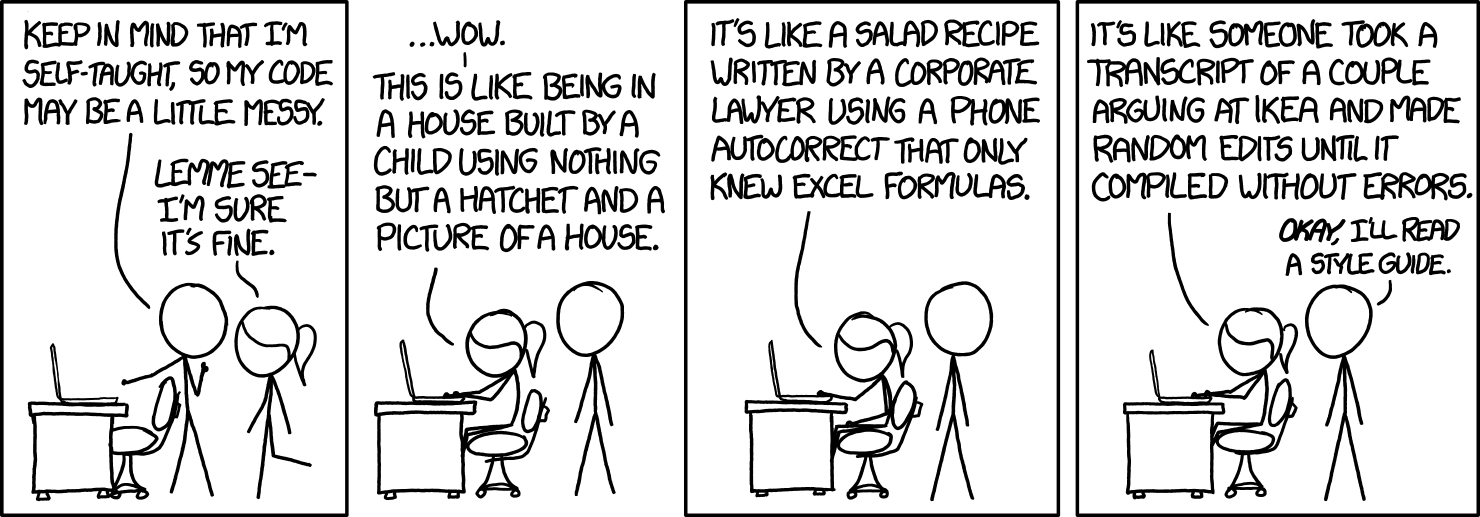
\includegraphics[width=0.9\textwidth,height=\textheight]{chapters/python/../../figures/code_quality_2x.png}

\section{Informazioni sull'Ambiente di
Sviluppo}\label{informazioni-sullambiente-di-sviluppo-1}

\begin{Shaded}
\begin{Highlighting}[]
\OperatorTok{\%}\NormalTok{load\_ext watermark}
\OperatorTok{\%}\NormalTok{watermark }\OperatorTok{{-}}\NormalTok{n }\OperatorTok{{-}}\NormalTok{u }\OperatorTok{{-}}\NormalTok{v }\OperatorTok{{-}}\NormalTok{iv }\OperatorTok{{-}}\NormalTok{w }\OperatorTok{{-}}\NormalTok{m}
\end{Highlighting}
\end{Shaded}

\begin{verbatim}
Last updated: Mon Jan 29 2024

Python implementation: CPython
Python version       : 3.11.7
IPython version      : 8.19.0

Compiler    : Clang 16.0.6 
OS          : Darwin
Release     : 23.3.0
Machine     : x86_64
Processor   : i386
CPU cores   : 8
Architecture: 64bit

pandas    : 2.1.4
numpy     : 1.26.2
seaborn   : 0.13.0
arviz     : 0.17.0
matplotlib: 3.8.2

Watermark: 2.4.3
\end{verbatim}

\chapter{NumPy}\label{sec-numpy}

La Standard Library di Python mette a disposizione un'ampia gamma di
funzioni utili per l'analisi dei dati. Tuttavia, per un'analisi più
approfondita ed efficiente, è raccomandato avvalersi di funzioni
specifiche disponibili in altri moduli esterni. Tra questi, i più
rilevanti per l'analisi dei dati includono NumPy, Pandas, Matplotlib e
Seaborn.

NumPy, abbreviazione di Numerical Python, rappresenta un'estensione del
linguaggio Python focalizzata sul calcolo algebrico e matriciale. Questo
modulo è essenziale per la maggior parte delle operazioni di calcolo
numerico in Python, poiché introduce strutture dati avanzate progettate
per l'elaborazione efficiente di vettori, matrici e insiemi di dati di
grandi dimensioni. Beneficiando dell'implementazione in linguaggi ad
alte prestazioni come C e Fortran, NumPy offre un'elevata efficienza,
specialmente in operazioni vettorializzate che sfruttano vettori e
matrici per formulare calcoli. Parallelamente, Pandas si afferma come
strumento fondamentale per l'importazione e la manipolazione dei dati,
mentre Matplotlib e Seaborn si distinguono per le loro capacità di
visualizzazione, facilitando notevolmente la creazione di
rappresentazioni grafiche dei dati. Questi moduli, combinati insieme,
costituiscono un ecosistema robusto e versatile per l'analisi e
l'elaborazione dei dati in Python.

In questo capitolo, introdurremo NumPy, che è ampiamente utilizzato in
quasi tutti i calcoli numerici in Python. NumPy consente di lavorare con
vettori e matrici in modo più efficiente e veloce rispetto alle liste e
alle liste di liste (utilizzate come matrici) di Python. Oltre a ciò,
NumPy fornisce una vasta gamma di funzioni matematiche di base, nonché
strumenti avanzati per la generazione di numeri casuali -- si veda
\textbf{?@sec-rng}.

\section{Preparazione del Notebook}\label{preparazione-del-notebook}

\begin{Shaded}
\begin{Highlighting}[]
\ImportTok{import}\NormalTok{ numpy }\ImportTok{as}\NormalTok{ np}
\end{Highlighting}
\end{Shaded}

\section{Utilizzo degli Array nel Modulo
NumPy}\label{utilizzo-degli-array-nel-modulo-numpy}

In Python standard, abbiamo a disposizione tipi di dati numerici (come
numeri interi e decimali) e strutture come liste, dizionari e insiemi.
NumPy, d'altro canto, introduce un nuovo tipo di struttura dati: l'array
N-dimensionale, noto come \texttt{ndarray}. Questi array hanno alcune
caratteristiche distintive:

\begin{itemize}
\tightlist
\item
  \textbf{Dimensioni}: Gli \texttt{ndarray} possono variare nel numero
  di dimensioni, definite come ``assi''. Ad esempio, un array può essere
  unidimensionale (simile a un vettore lineare), bidimensionale (come
  una matrice o una tabella), tridimensionale (simile a un cubo), e così
  via.
\item
  \textbf{Tipo di Dato}: A differenza delle liste in Python standard che
  possono contenere diversi tipi di dati, ogni elemento all'interno di
  un \texttt{ndarray} deve essere dello stesso tipo, come numeri interi,
  decimali, booleani o stringhe.
\item
  \textbf{Forma}: La ``forma'' di un \texttt{ndarray} si riferisce alle
  sue dimensioni, ovvero quante righe, colonne o altri livelli di
  profondità ha. Per esempio, la forma (3, 4) indica un array con 3
  righe e 4 colonne.
\item
  \textbf{Indicizzazione}: Gli \texttt{ndarray} possono essere
  indicizzati in modo simile agli array standard di Python, ma offrono
  anche opzioni più avanzate per l'indicizzazione.
\end{itemize}

Gli \texttt{ndarray} sono potenti per manipolare e analizzare i dati,
grazie alle loro funzioni e metodi che includono operazioni matematiche
e statistiche, trasformazioni e altre manipolazioni dei dati.

\textbf{Terminologia Importante:} - \textbf{Size}: Indica il numero
totale di elementi in un array. - \textbf{Rank}: Si riferisce al numero
di dimensioni, o assi, di un array. - \textbf{Shape}: Denota le
dimensioni specifiche dell'array, ovvero una sequenza di numeri che
rappresentano il conteggio degli elementi in ogni dimensione.

\textbf{Come Creare un \texttt{ndarray}:} Il modo più diretto per creare
un \texttt{ndarray} è attraverso la conversione di una lista Python. Ad
esempio, è possibile creare un array unidimensionale (1-D) a partire da
una lista standard di Python.

\begin{Shaded}
\begin{Highlighting}[]
\NormalTok{x }\OperatorTok{=}\NormalTok{ np.array([}\DecValTok{1}\NormalTok{, }\DecValTok{2}\NormalTok{, }\DecValTok{3}\NormalTok{, }\DecValTok{4}\NormalTok{, }\DecValTok{5}\NormalTok{, }\DecValTok{6}\NormalTok{])}
\end{Highlighting}
\end{Shaded}

L'istruzione precedente crea un array in NumPy, assegnandolo alla
variabile \texttt{x}. Questo array è un vettore unidimensionale
contenente sei elementi, che sono i numeri interi specificati
all'interno delle parentesi quadre.

\begin{Shaded}
\begin{Highlighting}[]
\BuiltInTok{print}\NormalTok{(x)}
\end{Highlighting}
\end{Shaded}

\begin{verbatim}
[1 2 3 4 5 6]
\end{verbatim}

\textbf{Indicizzazione}

Se vogliamo estrarre un singolo elemento del vettore lo indicizziamo con
la sua posizione (si ricordi che l'indice inizia da 0):

\begin{Shaded}
\begin{Highlighting}[]
\NormalTok{x[}\DecValTok{0}\NormalTok{]}
\end{Highlighting}
\end{Shaded}

\begin{verbatim}
1
\end{verbatim}

\begin{Shaded}
\begin{Highlighting}[]
\NormalTok{x[}\DecValTok{2}\NormalTok{]}
\end{Highlighting}
\end{Shaded}

\begin{verbatim}
3
\end{verbatim}

Un array 2-D si crea nel modo seguente:

\begin{Shaded}
\begin{Highlighting}[]
\NormalTok{y }\OperatorTok{=}\NormalTok{ np.array([[}\DecValTok{1}\NormalTok{, }\DecValTok{2}\NormalTok{, }\DecValTok{3}\NormalTok{, }\DecValTok{4}\NormalTok{], [}\DecValTok{5}\NormalTok{, }\DecValTok{6}\NormalTok{, }\DecValTok{7}\NormalTok{, }\DecValTok{8}\NormalTok{], [}\DecValTok{9}\NormalTok{, }\DecValTok{10}\NormalTok{, }\DecValTok{11}\NormalTok{, }\DecValTok{12}\NormalTok{]])}
\BuiltInTok{print}\NormalTok{(y)}
\end{Highlighting}
\end{Shaded}

\begin{verbatim}
[[ 1  2  3  4]
 [ 5  6  7  8]
 [ 9 10 11 12]]
\end{verbatim}

Estraiamo un singolo elemento dall'array:

\begin{Shaded}
\begin{Highlighting}[]
\NormalTok{y[}\DecValTok{0}\NormalTok{, }\DecValTok{2}\NormalTok{]}
\end{Highlighting}
\end{Shaded}

\begin{verbatim}
3
\end{verbatim}

Estraiamo la seconda riga dall'array:

\begin{Shaded}
\begin{Highlighting}[]
\NormalTok{y[}\DecValTok{1}\NormalTok{]}
\end{Highlighting}
\end{Shaded}

\begin{verbatim}
array([5, 6, 7, 8])
\end{verbatim}

Estraiamo la seconda colonna dall'array:

\begin{Shaded}
\begin{Highlighting}[]
\NormalTok{y[:, }\DecValTok{1}\NormalTok{] }
\end{Highlighting}
\end{Shaded}

\begin{verbatim}
array([ 2,  6, 10])
\end{verbatim}

La sintassi con i due punti è chiamata ``slicing'' dell'array.

\begin{Shaded}
\begin{Highlighting}[]
\CommentTok{\# Display the first row of the array}
\BuiltInTok{print}\NormalTok{(}\StringTok{"Displaying the first row:"}\NormalTok{)}
\BuiltInTok{print}\NormalTok{(y[}\DecValTok{0}\NormalTok{, :])}
\end{Highlighting}
\end{Shaded}

\begin{verbatim}
Displaying the first row:
[1 2 3 4]
\end{verbatim}

\begin{Shaded}
\begin{Highlighting}[]
\CommentTok{\# Show the last two elements in the first row}
\BuiltInTok{print}\NormalTok{(}\StringTok{"Showing the last two elements in the first row:"}\NormalTok{)}
\BuiltInTok{print}\NormalTok{(y[}\DecValTok{0}\NormalTok{, }\OperatorTok{{-}}\DecValTok{2}\NormalTok{:])}
\end{Highlighting}
\end{Shaded}

\begin{verbatim}
Showing the last two elements in the first row:
[3 4]
\end{verbatim}

\begin{Shaded}
\begin{Highlighting}[]
\CommentTok{\# Retrieve every second element in the first row}
\BuiltInTok{print}\NormalTok{(}\StringTok{"Retrieving every second element in the first row:"}\NormalTok{)}
\BuiltInTok{print}\NormalTok{(y[}\DecValTok{0}\NormalTok{, ::}\DecValTok{2}\NormalTok{])}
\end{Highlighting}
\end{Shaded}

\begin{verbatim}
Retrieving every second element in the first row:
[1 3]
\end{verbatim}

\begin{Shaded}
\begin{Highlighting}[]
\CommentTok{\# Extract a submatrix from the original array}
\BuiltInTok{print}\NormalTok{(}\StringTok{"Extracting a submatrix:"}\NormalTok{)}
\BuiltInTok{print}\NormalTok{(y[:}\DecValTok{2}\NormalTok{, }\DecValTok{1}\NormalTok{:}\DecValTok{3}\NormalTok{])}
\end{Highlighting}
\end{Shaded}

\begin{verbatim}
Extracting a submatrix:
[[2 3]
 [6 7]]
\end{verbatim}

\subsection{\texorpdfstring{Funzioni per
\texttt{ndarray}}{Funzioni per ndarray}}\label{funzioni-per-ndarray}

Numpy offre varie funzioni per creare \texttt{ndarray}. Per esempio, è
possibile creare un array 1-D con la funzione
\texttt{.arange(start,\ stop,\ incr,\ dtype=..)} che fornisce
l'intervallo di numeri compreso fra \texttt{start}, \texttt{stop}, al
passo \texttt{incr}:

\begin{Shaded}
\begin{Highlighting}[]
\NormalTok{z }\OperatorTok{=}\NormalTok{ np.arange(}\DecValTok{2}\NormalTok{, }\DecValTok{9}\NormalTok{, }\DecValTok{2}\NormalTok{)}
\BuiltInTok{print}\NormalTok{(z)}
\end{Highlighting}
\end{Shaded}

\begin{verbatim}
[2 4 6 8]
\end{verbatim}

Si usa spesso \texttt{.arange} per creare sequenze a incrementi unitari:

\begin{Shaded}
\begin{Highlighting}[]
\NormalTok{w }\OperatorTok{=}\NormalTok{ np.arange(}\DecValTok{11}\NormalTok{)}
\BuiltInTok{print}\NormalTok{(w)}
\end{Highlighting}
\end{Shaded}

\begin{verbatim}
[ 0  1  2  3  4  5  6  7  8  9 10]
\end{verbatim}

Un'altra funzione molto utile è \texttt{.linspace}:

\begin{Shaded}
\begin{Highlighting}[]
\NormalTok{x }\OperatorTok{=}\NormalTok{ np.linspace(}\DecValTok{0}\NormalTok{, }\DecValTok{10}\NormalTok{, num}\OperatorTok{=}\DecValTok{20}\NormalTok{)}
\BuiltInTok{print}\NormalTok{(x)}
\end{Highlighting}
\end{Shaded}

\begin{verbatim}
[ 0.          0.52631579  1.05263158  1.57894737  2.10526316  2.63157895
  3.15789474  3.68421053  4.21052632  4.73684211  5.26315789  5.78947368
  6.31578947  6.84210526  7.36842105  7.89473684  8.42105263  8.94736842
  9.47368421 10.        ]
\end{verbatim}

Fissati gli estremi (qui 0, 10) e il numero di elementi desiderati,
\texttt{.linspace} determina in maniera automatica l'incremento.

Una proprietà molto utile dei \texttt{ndarray} è la possibilità di
filtrare gli elementi di un array che rispondono come \texttt{True} ad
un criterio. Per esempio:

\begin{Shaded}
\begin{Highlighting}[]
\BuiltInTok{print}\NormalTok{(x[x }\OperatorTok{\textgreater{}} \DecValTok{7}\NormalTok{])}
\end{Highlighting}
\end{Shaded}

\begin{verbatim}
[ 7.36842105  7.89473684  8.42105263  8.94736842  9.47368421 10.        ]
\end{verbatim}

perché solo gli ultimi sei elementi di \texttt{x} rispondono
\texttt{True} al criterio \(x > 7\).

Le dimensioni (``assi'') di un \texttt{ndarray} vengono ritornate dal
metodo \texttt{.dim}. Per esempio:

\begin{Shaded}
\begin{Highlighting}[]
\BuiltInTok{print}\NormalTok{(y)}
\end{Highlighting}
\end{Shaded}

\begin{verbatim}
[[ 1  2  3  4]
 [ 5  6  7  8]
 [ 9 10 11 12]]
\end{verbatim}

\begin{Shaded}
\begin{Highlighting}[]
\NormalTok{y.ndim}
\end{Highlighting}
\end{Shaded}

\begin{verbatim}
2
\end{verbatim}

\begin{Shaded}
\begin{Highlighting}[]
\BuiltInTok{print}\NormalTok{(y.}\BuiltInTok{max}\NormalTok{(axis}\OperatorTok{=}\DecValTok{1}\NormalTok{))}
\end{Highlighting}
\end{Shaded}

\begin{verbatim}
[ 4  8 12]
\end{verbatim}

\begin{Shaded}
\begin{Highlighting}[]
\BuiltInTok{print}\NormalTok{(y.}\BuiltInTok{max}\NormalTok{(axis}\OperatorTok{=}\DecValTok{0}\NormalTok{))}
\end{Highlighting}
\end{Shaded}

\begin{verbatim}
[ 9 10 11 12]
\end{verbatim}

Il numero di elementi per ciascun asse viene ritornato dal metodo
\texttt{.shape}:

\begin{Shaded}
\begin{Highlighting}[]
\NormalTok{y.shape}
\end{Highlighting}
\end{Shaded}

\begin{verbatim}
(3, 4)
\end{verbatim}

\section{Manipolazione di Array con
NumPy}\label{manipolazione-di-array-con-numpy}

NumPy rende più agevole lavorare con grandi quantità di dati. Un
concetto fondamentale in NumPy sono gli array monodimensionali, spesso
utilizzati per rappresentare vettori, ovvero sequenze di numeri che
possono rappresentare, ad esempio, le misurazioni di una variabile
specifica. Grazie a NumPy, possiamo eseguire operazioni aritmetiche su
questi vettori in modo semplice, applicando la stessa operazione a tutti
gli elementi dell'array contemporaneamente.

\subsection{Cosa Significa Vettorizzare
un'Operazione}\label{cosa-significa-vettorizzare-unoperazione}

La vettorizzazione è una delle funzionalità più efficaci di NumPy.
Quando diciamo che un'operazione è vettorizzata, significa che questa
operazione viene applicata in un colpo solo a tutti gli elementi
dell'array, invece di dover agire su ciascun elemento individualmente.
Questo approccio rende la manipolazione di grandi insiemi di dati non
solo più veloce ma anche più intuitiva, poiché consente di trattare
l'intero insieme di dati come un'unica entità anziché come una serie di
punti dati individuali.

Supponiamo di avere raccolto i dati di 4 individui

\begin{Shaded}
\begin{Highlighting}[]
\NormalTok{m }\OperatorTok{=}\NormalTok{ np.array([}\FloatTok{1.62}\NormalTok{, }\FloatTok{1.75}\NormalTok{, }\FloatTok{1.55}\NormalTok{, }\FloatTok{1.74}\NormalTok{])}
\NormalTok{kg }\OperatorTok{=}\NormalTok{ np.array([}\FloatTok{55.4}\NormalTok{, }\FloatTok{73.6}\NormalTok{, }\FloatTok{57.1}\NormalTok{, }\FloatTok{59.5}\NormalTok{])}

\BuiltInTok{print}\NormalTok{(m)}
\BuiltInTok{print}\NormalTok{(kg)}
\end{Highlighting}
\end{Shaded}

\begin{verbatim}
[1.62 1.75 1.55 1.74]
[55.4 73.6 57.1 59.5]
\end{verbatim}

dove \texttt{m} è l'array che contiene i dati relativi all'altezza in
metri dei quattro individui e \texttt{kg} è l'array che contiene i dati
relativi al peso in kg. I dati sono organizzati in modo tale che il
primo elemento di entrambi i vettori si riferisce alle misure del primo
individuo, il secondo elemento dei due vettori si riferisce alle misure
del secondo individuo, ecc.

Supponiamo di volere calcolare l'indice BMI:

\[
BMI = \frac{kg}{m^2}.
\]

Per il primo individuo del campione, l'indice di massa corporea è

\begin{Shaded}
\begin{Highlighting}[]
\FloatTok{55.4} \OperatorTok{/} \FloatTok{1.62}\OperatorTok{**}\DecValTok{2}
\end{Highlighting}
\end{Shaded}

\begin{verbatim}
21.109586953208346
\end{verbatim}

Si noti che non abbiamo bisogno di scrivere \texttt{55.4\ /\ (1.62**2)}
in quanto, in Python, l'elevazione a potenza viene eseguita prima della
somma e della divisione (come in tutti i linguaggi). Usando i dati
immagazzinati nei due vettori, lo stesso risultato si ottiene nel modo
seguente:

\begin{Shaded}
\begin{Highlighting}[]
\NormalTok{kg[}\DecValTok{0}\NormalTok{] }\OperatorTok{/}\NormalTok{ m[}\DecValTok{0}\NormalTok{]}\OperatorTok{**}\DecValTok{2}
\end{Highlighting}
\end{Shaded}

\begin{verbatim}
21.109586953208346
\end{verbatim}

Se ora non specifichiamo l'indice (per esempio, \texttt{{[}0{]}}), le
operazioni aritmetiche indicate verranno eseguite \emph{per ciascuna
coppia} di elementi corrispondenti nei due vettori:

\begin{Shaded}
\begin{Highlighting}[]
\NormalTok{bmi }\OperatorTok{=}\NormalTok{ kg }\OperatorTok{/}\NormalTok{ m}\OperatorTok{**}\DecValTok{2}
\end{Highlighting}
\end{Shaded}

Otteniamo così, con una sola istruzione, l'indice BMI dei quattro
individui:

\begin{Shaded}
\begin{Highlighting}[]
\NormalTok{bmi.}\BuiltInTok{round}\NormalTok{(}\DecValTok{1}\NormalTok{)}
\end{Highlighting}
\end{Shaded}

\begin{verbatim}
array([21.1, 24. , 23.8, 19.7])
\end{verbatim}

Questo esempio illustra come le operazioni aritmetiche standard vengano
eseguite elemento per elemento negli array, grazie al processo di
vettorizzazione.

\section{Broadcasting}\label{broadcasting}

Il broadcasting è una caratteristica distintiva di NumPy che facilita
l'esecuzione di operazioni tra array di dimensioni diverse o tra un
array e uno scalare, anche se le loro dimensioni non sono direttamente
compatibili. Grazie al broadcasting, NumPy è in grado di ``espandere''
automaticamente le dimensioni di uno degli operandi per rendere
possibile l'operazione.

Questo significa che possiamo, per esempio, eseguire un'operazione tra
un array e un numero singolo (un vettore e uno scalare) o tra due array
di dimensioni differenti, senza la necessità di modificare manualmente
le dimensioni di questi array. Il broadcasting si occupa di adattare le
dimensioni in modo coerente per consentire l'operazione desiderata. Ciò
rende il codice più snello e leggibile, eliminando la necessità di
espandere gli array manualmente.

In breve, il broadcasting in NumPy è un potente strumento che semplifica
l'esecuzione di operazioni su array di dimensioni diverse o tra array e
scalari, automatizzando l'allineamento delle dimensioni.

\subsection{Esempio di Broadcasting}\label{esempio-di-broadcasting}

Immaginiamo di avere un array \texttt{A} con dimensioni 3x3 e un numero
scalare \texttt{B}. Senza broadcasting, dovremmo espandere \texttt{B} in
un array 3x3 riempiendo ogni cella con il valore di \texttt{B} per
eseguire un'operazione come l'addizione su ciascun elemento di
\texttt{A}. Grazie al broadcasting, possiamo semplicemente scrivere
\texttt{A\ +\ B}, e NumPy si occuperà automaticamente di ``espandere''
\texttt{B} durante l'operazione, applicando il valore scalare a ogni
elemento di \texttt{A}.

\begin{Shaded}
\begin{Highlighting}[]
\CommentTok{\# Creiamo un array 3x3}
\NormalTok{A }\OperatorTok{=}\NormalTok{ np.array([[}\DecValTok{1}\NormalTok{, }\DecValTok{2}\NormalTok{, }\DecValTok{3}\NormalTok{], [}\DecValTok{4}\NormalTok{, }\DecValTok{5}\NormalTok{, }\DecValTok{6}\NormalTok{], [}\DecValTok{7}\NormalTok{, }\DecValTok{8}\NormalTok{, }\DecValTok{9}\NormalTok{]])}

\CommentTok{\# Definiamo uno scalare}
\NormalTok{B }\OperatorTok{=} \DecValTok{5}

\CommentTok{\# Applichiamo il broadcasting per aggiungere lo scalare a ogni elemento dell\textquotesingle{}array}
\NormalTok{C }\OperatorTok{=}\NormalTok{ A }\OperatorTok{+}\NormalTok{ B}

\BuiltInTok{print}\NormalTok{(C)}
\end{Highlighting}
\end{Shaded}

\begin{verbatim}
[[ 6  7  8]
 [ 9 10 11]
 [12 13 14]]
\end{verbatim}

In questo esempio, \texttt{C} conterrà l'array originale \texttt{A} con
ogni elemento incrementato di 5, dimostrando come il broadcasting
semplifichi operazioni che altrimenti richiederebbero passaggi
aggiuntivi.

\section{Altre operazioni sugli
array}\label{altre-operazioni-sugli-array}

C'è un numero enorme di funzioni predefinite in NumPy che calcolano
automaticamente diverse quantità sugli \texttt{ndarray}. Ad esempio:

\begin{itemize}
\tightlist
\item
  \texttt{mean()}: calcola la media di un vettore o matrice;
\item
  \texttt{sum()}: calcola la somma di un vettore o matrice;
\item
  \texttt{std()}: calcola la deviazione standard;
\item
  \texttt{min()}: trova il minimo nel vettore o matrice;
\item
  \texttt{max()}: trova il massimo;
\item
  \texttt{ndim}: dimensione del vettore o matrice;
\item
  \texttt{shape}: restituisce una tupla con la ``forma'' del vettore o
  matrice;
\item
  \texttt{size}: restituisce la dimensione totale del vettore (=ndim) o
  della matrice;
\item
  \texttt{dtype}: scrive il tipo numpy del dato;
\item
  \texttt{zeros(num)}: scrive un vettore di num elementi inizializzati a
  zero;
\item
  \texttt{arange(start,stop,step)}: genera un intervallo di valori
  (interi o reali, a seconda dei valori di start, ecc.) intervallati di
  step. Nota che i dati vengono generati nell'intervallo aperto
  {[}start,stop)!
\item
  \texttt{linstep(start,stop,num)}: genera un intervallo di num valori
  interi o reali a partire da start fino a stop (incluso!);
\item
  \texttt{astype(tipo)}: converte l'ndarray nel tipo specificato
\end{itemize}

Per esempio:

\begin{Shaded}
\begin{Highlighting}[]
\NormalTok{x }\OperatorTok{=}\NormalTok{ np.array([}\DecValTok{1}\NormalTok{, }\DecValTok{2}\NormalTok{, }\DecValTok{3}\NormalTok{])}
\BuiltInTok{print}\NormalTok{(x)}
\end{Highlighting}
\end{Shaded}

\begin{verbatim}
[1 2 3]
\end{verbatim}

\begin{Shaded}
\begin{Highlighting}[]
\NormalTok{[x.}\BuiltInTok{min}\NormalTok{(), x.}\BuiltInTok{max}\NormalTok{(), x.}\BuiltInTok{sum}\NormalTok{(), x.mean(), x.std()]}
\end{Highlighting}
\end{Shaded}

\begin{verbatim}
[1, 3, 6, 2.0, 0.816496580927726]
\end{verbatim}

\section{Lavorare con formule
matematiche}\label{lavorare-con-formule-matematiche}

L'implementazione delle formule matematiche sugli array è un processo
molto semplice con Numpy. Possiamo prendere ad esempio la formula della
deviazione standard che discuteremo nel capitolo
\{ref\}\texttt{loc-scale-notebook}:

\[
s = \sqrt{\sum_{i=1}^n\frac{(x_i - \bar{x})^2}{n}}
\]

L'implementazione su un array NumPy è la seguente:

\begin{Shaded}
\begin{Highlighting}[]
\BuiltInTok{print}\NormalTok{(x)}
\end{Highlighting}
\end{Shaded}

\begin{verbatim}
[1 2 3]
\end{verbatim}

\begin{Shaded}
\begin{Highlighting}[]
\NormalTok{np.sqrt(np.}\BuiltInTok{sum}\NormalTok{((x }\OperatorTok{{-}}\NormalTok{ np.mean(x)) }\OperatorTok{**} \DecValTok{2}\NormalTok{) }\OperatorTok{/}\NormalTok{ np.size(x))}
\end{Highlighting}
\end{Shaded}

\begin{verbatim}
0.816496580927726
\end{verbatim}

Questa implementazione funziona nello stesso modo sia che \texttt{x}
contenga 3 elementi (come nel caso presente) sia che \texttt{x} contenga
migliaia di elementi. È importante notare l'utilizzo delle parentesi
tonde per specificare l'ordine di esecuzione delle operazioni. In
particolare, nel codice fornito, si inizia calcolando la media degli
elementi del vettore \texttt{x} per mezzo della funzione
\texttt{np.mean(x)}. Questa operazione produce uno scalare, ovvero un
singolo valore numerico che rappresenta la media degli elementi del
vettore. L'utilizzo delle parentesi tonde è fondamentale per garantire
l'ordine corretto delle operazioni. In questo caso, la funzione
\texttt{np.mean()} viene applicata al vettore \texttt{x} prima di
qualsiasi altra operazione matematica. Senza le parentesi tonde, le
operazioni verrebbero eseguite in un ordine diverso e il risultato
potrebbe essere errato.

\begin{Shaded}
\begin{Highlighting}[]
\NormalTok{np.mean(x)}
\end{Highlighting}
\end{Shaded}

\begin{verbatim}
2.0
\end{verbatim}

Successivamente, eseguiamo la sottrazione dei singoli elementi del
vettore \texttt{x} per la media del vettore stesso, ovvero
\(x_i - \bar{x}\), utilizzando il meccanismo del broadcasting.

\begin{Shaded}
\begin{Highlighting}[]
\NormalTok{x }\OperatorTok{{-}}\NormalTok{ np.mean(x)}
\end{Highlighting}
\end{Shaded}

\begin{verbatim}
array([-1.,  0.,  1.])
\end{verbatim}

Eleviamo poi al quadrato gli elementi del vettore che abbiamo ottenuto:

\begin{Shaded}
\begin{Highlighting}[]
\NormalTok{(x }\OperatorTok{{-}}\NormalTok{ np.mean(x)) }\OperatorTok{**} \DecValTok{2}
\end{Highlighting}
\end{Shaded}

\begin{verbatim}
array([1., 0., 1.])
\end{verbatim}

Sommiamo gli elementi del vettore:

\begin{Shaded}
\begin{Highlighting}[]
\NormalTok{np.}\BuiltInTok{sum}\NormalTok{((x }\OperatorTok{{-}}\NormalTok{ np.mean(x)) }\OperatorTok{**} \DecValTok{2}\NormalTok{)}
\end{Highlighting}
\end{Shaded}

\begin{verbatim}
2.0
\end{verbatim}

Dividiamo il numero ottenuto per \(n\). Questa è la varianza di \(x\):

\begin{Shaded}
\begin{Highlighting}[]
\NormalTok{res }\OperatorTok{=}\NormalTok{ np.}\BuiltInTok{sum}\NormalTok{((x }\OperatorTok{{-}}\NormalTok{ np.mean(x)) }\OperatorTok{**} \DecValTok{2}\NormalTok{) }\OperatorTok{/}\NormalTok{ np.size(x)}
\NormalTok{res}
\end{Highlighting}
\end{Shaded}

\begin{verbatim}
0.6666666666666666
\end{verbatim}

Infine, per ottenere la deviazione standard, prendiamo la radice
quadrata:

\begin{Shaded}
\begin{Highlighting}[]
\NormalTok{np.sqrt(res)}
\end{Highlighting}
\end{Shaded}

\begin{verbatim}
0.816496580927726
\end{verbatim}

Il risultato ottenuto coincide con quello che si trova applicando la
funzione \texttt{np.std()}:

\begin{Shaded}
\begin{Highlighting}[]
\NormalTok{np.std(x)}
\end{Highlighting}
\end{Shaded}

\begin{verbatim}
0.816496580927726
\end{verbatim}

\section{Slicing}\label{slicing}

Per concludere, spendiamo ancora alcune parole sull'indicizzazione degli
\texttt{ndarray}.

Slicing in Numpy è un meccanismo che consente di selezionare una
porzione di un array multidimensionale, ovvero una sotto-matrice o un
sotto-vettore. Per selezionare una porzione di un array, si utilizza la
sintassi \texttt{{[}start:stop:step{]}}, dove \texttt{start} indica
l'indice di partenza della porzione, \texttt{stop} indica l'indice di
fine e \texttt{step} indica il passo da utilizzare per la selezione. Se
uno o più di questi valori vengono omessi, vengono utilizzati dei valori
di default.

Ad esempio, se abbiamo un array \texttt{arr} di dimensione (3, 4) e
vogliamo selezionare la seconda colonna, possiamo usare la sintassi
\texttt{arr{[}:,\ 1{]}}. In questo caso, il simbolo \texttt{:} indica
che vogliamo selezionare tutte le righe, mentre il numero \texttt{1}
indica che vogliamo selezionare la seconda colonna.

Inoltre, possiamo utilizzare il meccanismo di slicing anche per
selezionare porzioni di array multidimensionali. Ad esempio, se abbiamo
un array \texttt{arr} di dimensione (3, 4, 5) e vogliamo selezionare la
prima riga di ciascuna matrice 4x5, possiamo usare la sintassi
\texttt{arr{[}:,\ 0,\ :{]}}.

Per esempio, creiamo l'array \texttt{x} di rango 2 con shape (3, 4):

\begin{Shaded}
\begin{Highlighting}[]
\NormalTok{x }\OperatorTok{=}\NormalTok{ np.array([[}\DecValTok{1}\NormalTok{, }\DecValTok{2}\NormalTok{, }\DecValTok{3}\NormalTok{, }\DecValTok{4}\NormalTok{], [}\DecValTok{5}\NormalTok{, }\DecValTok{6}\NormalTok{, }\DecValTok{7}\NormalTok{, }\DecValTok{8}\NormalTok{], [}\DecValTok{9}\NormalTok{, }\DecValTok{10}\NormalTok{, }\DecValTok{11}\NormalTok{, }\DecValTok{12}\NormalTok{]])}
\BuiltInTok{print}\NormalTok{(x)}
\end{Highlighting}
\end{Shaded}

\begin{verbatim}
[[ 1  2  3  4]
 [ 5  6  7  8]
 [ 9 10 11 12]]
\end{verbatim}

Utilizziamo il meccanismo di slicing per estrarre la sottomatrice
composta dalle prime 2 righe e dalle colonne 1 e 2. \texttt{y} è l'array
risultante di dimensione (2, 2):

\begin{Shaded}
\begin{Highlighting}[]
\NormalTok{y }\OperatorTok{=}\NormalTok{ x[:}\DecValTok{2}\NormalTok{, }\DecValTok{1}\NormalTok{:}\DecValTok{3}\NormalTok{]}
\BuiltInTok{print}\NormalTok{(y)}
\end{Highlighting}
\end{Shaded}

\begin{verbatim}
[[2 3]
 [6 7]]
\end{verbatim}

È importante sapere che uno slice di un array in Numpy è una vista degli
stessi dati, il che significa che modificarlo implica la modifica
dell'array originale. In pratica, quando si modifica uno slice di un
array, si sta modificando direttamente l'array originale e tutte le
altre visualizzazioni dell'array vedranno la stessa modifica. Questo
avviene perché Numpy è progettato per gestire enormi quantità di dati,
pertanto cerca di evitare il più possibile di effettuare copie dei dati.

Questo comportamento deve essere preso in considerazione durante la
modifica degli array in Numpy, al fine di evitare modifiche accidentali
o indesiderate. In alcuni casi, è possibile utilizzare il metodo
\texttt{copy()} per creare una copia indipendente di un array e lavorare
sulla copia senza modificare l'originale. Vediamo un esempio.

\begin{Shaded}
\begin{Highlighting}[]
\BuiltInTok{print}\NormalTok{(x[}\DecValTok{0}\NormalTok{, }\DecValTok{1}\NormalTok{])   }
\end{Highlighting}
\end{Shaded}

\begin{verbatim}
2
\end{verbatim}

\begin{Shaded}
\begin{Highlighting}[]
\NormalTok{y[}\DecValTok{0}\NormalTok{, }\DecValTok{0}\NormalTok{] }\OperatorTok{=} \DecValTok{77}     
\end{Highlighting}
\end{Shaded}

\begin{Shaded}
\begin{Highlighting}[]
\BuiltInTok{print}\NormalTok{(x)}
\end{Highlighting}
\end{Shaded}

\begin{verbatim}
[[ 1 77  3  4]
 [ 5  6  7  8]
 [ 9 10 11 12]]
\end{verbatim}

\begin{Shaded}
\begin{Highlighting}[]
\NormalTok{x }\OperatorTok{=}\NormalTok{ np.array([[}\DecValTok{1}\NormalTok{, }\DecValTok{2}\NormalTok{, }\DecValTok{3}\NormalTok{, }\DecValTok{4}\NormalTok{], [}\DecValTok{5}\NormalTok{, }\DecValTok{6}\NormalTok{, }\DecValTok{7}\NormalTok{, }\DecValTok{8}\NormalTok{], [}\DecValTok{9}\NormalTok{, }\DecValTok{10}\NormalTok{, }\DecValTok{11}\NormalTok{, }\DecValTok{12}\NormalTok{]])}

\NormalTok{z }\OperatorTok{=}\NormalTok{ x.copy()}
\BuiltInTok{print}\NormalTok{(z)}
\end{Highlighting}
\end{Shaded}

\begin{verbatim}
[[ 1  2  3  4]
 [ 5  6  7  8]
 [ 9 10 11 12]]
\end{verbatim}

\begin{Shaded}
\begin{Highlighting}[]
\NormalTok{z[}\DecValTok{0}\NormalTok{, }\DecValTok{1}\NormalTok{] }\OperatorTok{=} \DecValTok{33}
\BuiltInTok{print}\NormalTok{(z)}
\end{Highlighting}
\end{Shaded}

\begin{verbatim}
[[ 1 33  3  4]
 [ 5  6  7  8]
 [ 9 10 11 12]]
\end{verbatim}

\begin{Shaded}
\begin{Highlighting}[]
\BuiltInTok{print}\NormalTok{(x)}
\end{Highlighting}
\end{Shaded}

\begin{verbatim}
[[ 1  2  3  4]
 [ 5  6  7  8]
 [ 9 10 11 12]]
\end{verbatim}

\section{Copia e ``Copia Profonda'' in
Python}\label{copia-e-copia-profonda-in-python}

In Python, per ottimizzare le prestazioni, le assegnazioni di solito non
copiano gli oggetti sottostanti. Questo è particolarmente importante, ad
esempio, quando gli oggetti vengono passati tra funzioni, per evitare
una quantità eccessiva di copie in memoria quando non sono necessarie
(questo approccio è noto tecnicamente come ``passaggio per
riferimento'').

Consideriamo il seguente esempio con un array \texttt{A}:

\begin{Shaded}
\begin{Highlighting}[]
\NormalTok{A }\OperatorTok{=}\NormalTok{ np.array([[}\DecValTok{1}\NormalTok{, }\DecValTok{2}\NormalTok{], [}\DecValTok{3}\NormalTok{, }\DecValTok{4}\NormalTok{]])}
\end{Highlighting}
\end{Shaded}

Se creiamo un nuovo riferimento \texttt{B} a \texttt{A}:

\begin{Shaded}
\begin{Highlighting}[]
\NormalTok{B }\OperatorTok{=}\NormalTok{ A}
\end{Highlighting}
\end{Shaded}

Ora \texttt{B} si riferisce allo stesso insieme di dati di \texttt{A}.
Se modifichiamo \texttt{B}, anche \texttt{A} viene modificato di
conseguenza:

\begin{Shaded}
\begin{Highlighting}[]
\NormalTok{B[}\DecValTok{0}\NormalTok{,}\DecValTok{0}\NormalTok{] }\OperatorTok{=} \DecValTok{10}
\end{Highlighting}
\end{Shaded}

Dopo questa modifica, sia \texttt{B} che \texttt{A} saranno:

\begin{Shaded}
\begin{Highlighting}[]
\BuiltInTok{print}\NormalTok{(A)}
\end{Highlighting}
\end{Shaded}

\begin{verbatim}
[[10  2]
 [ 3  4]]
\end{verbatim}

Se desideriamo evitare questo comportamento, in modo tale che \texttt{B}
diventi un oggetto completamente indipendente da \texttt{A}, dobbiamo
effettuare una cosiddetta ``copia profonda'' utilizzando la funzione
\texttt{copy}:

\begin{Shaded}
\begin{Highlighting}[]
\NormalTok{B }\OperatorTok{=}\NormalTok{ np.copy(A)}
\end{Highlighting}
\end{Shaded}

Ora, se modificassimo \texttt{B}, \texttt{A} non subirebbe alcuna
modifica. Ad esempio:

\begin{Shaded}
\begin{Highlighting}[]
\NormalTok{B[}\DecValTok{0}\NormalTok{,}\DecValTok{0}\NormalTok{] }\OperatorTok{=} \OperatorTok{{-}}\DecValTok{5}
\end{Highlighting}
\end{Shaded}

A questo punto, \texttt{B} sarà:

\begin{Shaded}
\begin{Highlighting}[]
\BuiltInTok{print}\NormalTok{(B)}
\end{Highlighting}
\end{Shaded}

\begin{verbatim}
[[-5  2]
 [ 3  4]]
\end{verbatim}

Ma \texttt{A} rimarrà invariato:

\begin{Shaded}
\begin{Highlighting}[]
\BuiltInTok{print}\NormalTok{(A)}
\end{Highlighting}
\end{Shaded}

\begin{verbatim}
[[10  2]
 [ 3  4]]
\end{verbatim}

Questo esempio mostra chiaramente la differenza tra una semplice
assegnazione, che crea un riferimento all'oggetto originale, e una
``copia profonda'', che crea un nuovo oggetto indipendente.

\section{Informazioni sull'Ambiente di
Sviluppo}\label{informazioni-sullambiente-di-sviluppo-2}

\begin{Shaded}
\begin{Highlighting}[]
\OperatorTok{\%}\NormalTok{load\_ext watermark}
\OperatorTok{\%}\NormalTok{watermark }\OperatorTok{{-}}\NormalTok{n }\OperatorTok{{-}}\NormalTok{u }\OperatorTok{{-}}\NormalTok{v }\OperatorTok{{-}}\NormalTok{iv }\OperatorTok{{-}}\NormalTok{w }\OperatorTok{{-}}\NormalTok{m}
\end{Highlighting}
\end{Shaded}

\begin{verbatim}
Last updated: Mon Jan 29 2024

Python implementation: CPython
Python version       : 3.11.7
IPython version      : 8.19.0

Compiler    : Clang 16.0.6 
OS          : Darwin
Release     : 23.3.0
Machine     : x86_64
Processor   : i386
CPU cores   : 8
Architecture: 64bit

numpy: 1.26.2

Watermark: 2.4.3
\end{verbatim}

\chapter{Pandas (1)}\label{sec-pandas-1}

\textbf{Prerequisiti}

\begin{itemize}
\tightlist
\item
  Consultare il capitolo 10 di
  \href{https://wesmckinney.com/book/data-aggregation.html}{Python for
  Data Analysis, 3E}.
\end{itemize}

\textbf{Concetti e Competenze Chiave}

\begin{itemize}
\tightlist
\item
  Comprendere e sapere usare \texttt{pd.Series()} e
  \texttt{pd.DataFrame()}.
\end{itemize}

\textbf{Preparazione del Notebook}

\begin{Shaded}
\begin{Highlighting}[]
\ImportTok{import}\NormalTok{ pandas }\ImportTok{as}\NormalTok{ pd}
\ImportTok{import}\NormalTok{ numpy }\ImportTok{as}\NormalTok{ np}

\CommentTok{\# Di default, Pandas mostrerà 60 righe e 20 colonne. }
\CommentTok{\# Modifichiamo qui le impostazioni di visualizzazione predefinite di Pandas per mostrare più righe.}
\NormalTok{pd.options.display.max\_rows }\OperatorTok{=} \DecValTok{100}
\end{Highlighting}
\end{Shaded}

\section*{Introduzione}\label{introduzione-1}
\addcontentsline{toc}{section}{Introduzione}

\markright{Introduzione}

La libreria \href{https://Pandas.pydata.org/docs/index.html}{Pandas}
offre diverse funzionalità per importare dati da fonti eterogenee, tra
cui fogli Excel, file CSV, JSON e database SQL.

Pandas si basa su due strutture dati principali:

\begin{itemize}
\tightlist
\item
  \textbf{Series}: utilizzata per rappresentare singole righe o colonne
  di un DataFrame, è simile a un array di NumPy.
\item
  \textbf{DataFrame}: una struttura dati simile a una tabella,
  organizzata in colonne, dove ciascuna riga rappresenta un'unità di
  osservazione con i relativi dati.
\end{itemize}

L'obiettivo di questo capitolo è imparare a usare i DataFrame e a
manipolare i dati al loro interno.

\section{Series}\label{series}

In Pandas, una \texttt{Series} è un array unidimensionale composto da
una sequenza di valori omogenei, simile ad un \emph{ndarray},
accompagnato da un array di etichette chiamato ``index''. A differenza
degli indici degli array Numpy, che sono sempre interi e partono da
zero, gli oggetti \texttt{Series} supportano etichette personalizzate
che possono essere, ad esempio, delle stringhe. Inoltre, gli oggetti
\texttt{Series} possono contenere dati mancanti che vengono ignorati da
molte delle operazioni della classe.

Il modo più semplice di creare un oggetto \texttt{Series} è di
convertire una lista. Per esempio:

\begin{Shaded}
\begin{Highlighting}[]
\NormalTok{grades }\OperatorTok{=}\NormalTok{ pd.Series([}\DecValTok{27}\NormalTok{, }\DecValTok{30}\NormalTok{, }\DecValTok{24}\NormalTok{, }\DecValTok{18}\NormalTok{, }\DecValTok{22}\NormalTok{, }\DecValTok{20}\NormalTok{, }\DecValTok{29}\NormalTok{])}
\end{Highlighting}
\end{Shaded}

È possibile ottenere la rappresentazione dell'\texttt{array}
dell'oggetto e dell'indice dell'oggetto \texttt{Series} tramite i suoi
attributi \texttt{array} e \texttt{index}, rispettivamente.

\begin{Shaded}
\begin{Highlighting}[]
\NormalTok{grades.array}
\end{Highlighting}
\end{Shaded}

\begin{verbatim}
<NumpyExtensionArray>
[27, 30, 24, 18, 22, 20, 29]
Length: 7, dtype: int64
\end{verbatim}

\begin{Shaded}
\begin{Highlighting}[]
\NormalTok{grades.index}
\end{Highlighting}
\end{Shaded}

\begin{verbatim}
RangeIndex(start=0, stop=7, step=1)
\end{verbatim}

Oppure, possiamo semplicemente stampare i contenuti dell'oggetto
\texttt{Series} direttamente:

\begin{Shaded}
\begin{Highlighting}[]
\BuiltInTok{print}\NormalTok{(grades)}
\end{Highlighting}
\end{Shaded}

\begin{verbatim}
0    27
1    30
2    24
3    18
4    22
5    20
6    29
dtype: int64
\end{verbatim}

Per accedere agli elementi di un oggetto \texttt{Series} si usano le
parentesi quadre contenenti un indice:

\begin{Shaded}
\begin{Highlighting}[]
\NormalTok{grades[}\DecValTok{0}\NormalTok{]}
\end{Highlighting}
\end{Shaded}

\begin{verbatim}
27
\end{verbatim}

\begin{Shaded}
\begin{Highlighting}[]
\NormalTok{grades[}\DecValTok{0}\NormalTok{:}\DecValTok{3}\NormalTok{]}
\end{Highlighting}
\end{Shaded}

\begin{verbatim}
0    27
1    30
2    24
dtype: int64
\end{verbatim}

È possibile filtrare gli elementi di un oggetto \texttt{Series} con un
array booleano:

\begin{Shaded}
\begin{Highlighting}[]
\NormalTok{grades }\OperatorTok{\textgreater{}} \DecValTok{24}
\end{Highlighting}
\end{Shaded}

\begin{verbatim}
0     True
1     True
2    False
3    False
4    False
5    False
6     True
dtype: bool
\end{verbatim}

\begin{Shaded}
\begin{Highlighting}[]
\NormalTok{grades[grades }\OperatorTok{\textgreater{}} \DecValTok{24}\NormalTok{]}
\end{Highlighting}
\end{Shaded}

\begin{verbatim}
0    27
1    30
6    29
dtype: int64
\end{verbatim}

È possibile manipolare gli elementi di un oggetto \texttt{Series} con le
normali operazioni aritmetiche mediante la vettorializzazione:

\begin{Shaded}
\begin{Highlighting}[]
\NormalTok{grades }\OperatorTok{/} \DecValTok{10}
\end{Highlighting}
\end{Shaded}

\begin{verbatim}
0    2.7
1    3.0
2    2.4
3    1.8
4    2.2
5    2.0
6    2.9
dtype: float64
\end{verbatim}

\begin{Shaded}
\begin{Highlighting}[]
\NormalTok{np.sqrt(grades)}
\end{Highlighting}
\end{Shaded}

\begin{verbatim}
0    5.196152
1    5.477226
2    4.898979
3    4.242641
4    4.690416
5    4.472136
6    5.385165
dtype: float64
\end{verbatim}

Gli oggetti \texttt{Series} hanno diversi metodi per svolgere varie
operazioni, per esempio per ricavare alcune statistiche descrittive:

\begin{Shaded}
\begin{Highlighting}[]
\NormalTok{[grades.count(), grades.mean(), grades.}\BuiltInTok{min}\NormalTok{(), grades.}\BuiltInTok{max}\NormalTok{(), grades.std(), grades.}\BuiltInTok{sum}\NormalTok{()]}
\end{Highlighting}
\end{Shaded}

\begin{verbatim}
[7, 24.285714285714285, 18, 30, 4.572172558506722, 170]
\end{verbatim}

Molto utile è il metodo \texttt{.describe()}:

\begin{Shaded}
\begin{Highlighting}[]
\NormalTok{grades.describe()}
\end{Highlighting}
\end{Shaded}

\begin{verbatim}
count     7.000000
mean     24.285714
std       4.572173
min      18.000000
25%      21.000000
50%      24.000000
75%      28.000000
max      30.000000
dtype: float64
\end{verbatim}

\section{DataFrame}\label{dataframe}

Un \texttt{pandas.DataFrame} è composto da righe e colonne. Ogni colonna
di un dataframe è un oggetto \texttt{pandas.Series}: quindi, un
dataframe è una collezione di serie. A differenza di un array NumPy, un
dataframe può combinare più tipi di dati, come numeri e testo, ma i dati
in ogni colonna sono dello stesso tipo.

Esistono molti modi per costruire un DataFrame. Un primo metodo è quello
di utilizzare un dizionario che include una o più liste o array Numpy di
uguale lunghezza. Per esempio:

\begin{Shaded}
\begin{Highlighting}[]
\NormalTok{data }\OperatorTok{=}\NormalTok{ \{}
    \StringTok{"name"}\NormalTok{: [}
        \StringTok{"Maria"}\NormalTok{,}
        \StringTok{"Anna"}\NormalTok{,}
        \StringTok{"Francesco"}\NormalTok{,}
        \StringTok{"Cristina"}\NormalTok{,}
        \StringTok{"Gianni"}\NormalTok{,}
        \StringTok{"Gabriella"}\NormalTok{,}
        \StringTok{"Stefano"}\NormalTok{,}
\NormalTok{    ],}
    \StringTok{"sex"}\NormalTok{: [}\StringTok{"f"}\NormalTok{, }\StringTok{"f"}\NormalTok{, }\StringTok{"m"}\NormalTok{, }\StringTok{"f"}\NormalTok{, }\StringTok{"m"}\NormalTok{, }\StringTok{"f"}\NormalTok{, }\StringTok{"m"}\NormalTok{],}
    \StringTok{"group"}\NormalTok{: [}\StringTok{"a"}\NormalTok{, }\StringTok{"b"}\NormalTok{, }\StringTok{"a"}\NormalTok{, }\StringTok{"b"}\NormalTok{, }\StringTok{"b"}\NormalTok{, }\StringTok{"c"}\NormalTok{, }\StringTok{"a"}\NormalTok{],}
    \StringTok{"x"}\NormalTok{: [}\DecValTok{1}\NormalTok{, }\DecValTok{2}\NormalTok{, }\DecValTok{3}\NormalTok{, }\DecValTok{4}\NormalTok{, }\DecValTok{5}\NormalTok{, }\DecValTok{6}\NormalTok{, }\DecValTok{7}\NormalTok{],}
    \StringTok{"y"}\NormalTok{: [}\DecValTok{8}\NormalTok{, }\DecValTok{9}\NormalTok{, }\DecValTok{10}\NormalTok{, }\DecValTok{11}\NormalTok{, }\DecValTok{12}\NormalTok{, }\DecValTok{13}\NormalTok{, }\DecValTok{14}\NormalTok{],}
    \StringTok{"z"}\NormalTok{: [}\DecValTok{15}\NormalTok{, }\DecValTok{16}\NormalTok{, }\DecValTok{17}\NormalTok{, }\DecValTok{18}\NormalTok{, }\DecValTok{19}\NormalTok{, }\DecValTok{20}\NormalTok{, }\DecValTok{21}\NormalTok{],}
\NormalTok{\}}
\NormalTok{frame }\OperatorTok{=}\NormalTok{ pd.DataFrame(data)}
\NormalTok{frame}
\end{Highlighting}
\end{Shaded}

\begin{longtable}[]{@{}lllllll@{}}
\toprule\noalign{}
& name & sex & group & x & y & z \\
\midrule\noalign{}
\endhead
\bottomrule\noalign{}
\endlastfoot
0 & Maria & f & a & 1 & 8 & 15 \\
1 & Anna & f & b & 2 & 9 & 16 \\
2 & Francesco & m & a & 3 & 10 & 17 \\
3 & Cristina & f & b & 4 & 11 & 18 \\
4 & Gianni & m & b & 5 & 12 & 19 \\
5 & Gabriella & f & c & 6 & 13 & 20 \\
6 & Stefano & m & a & 7 & 14 & 21 \\
\end{longtable}

Oppure possiamo procedere nel modo seguente:

\begin{Shaded}
\begin{Highlighting}[]
\NormalTok{df }\OperatorTok{=}\NormalTok{ pd.DataFrame()}

\NormalTok{df[}\StringTok{"x"}\NormalTok{] }\OperatorTok{=}\NormalTok{ [}\DecValTok{1}\NormalTok{, }\DecValTok{2}\NormalTok{, }\DecValTok{3}\NormalTok{, }\DecValTok{4}\NormalTok{, }\DecValTok{5}\NormalTok{, }\DecValTok{6}\NormalTok{, }\DecValTok{7}\NormalTok{]}
\NormalTok{df[}\StringTok{"y"}\NormalTok{] }\OperatorTok{=}\NormalTok{ [}\DecValTok{8}\NormalTok{, }\DecValTok{9}\NormalTok{, }\DecValTok{10}\NormalTok{, }\DecValTok{11}\NormalTok{, }\DecValTok{12}\NormalTok{, }\DecValTok{13}\NormalTok{, }\DecValTok{14}\NormalTok{]}
\NormalTok{df[}\StringTok{"z"}\NormalTok{] }\OperatorTok{=}\NormalTok{ [}\FloatTok{14.4}\NormalTok{, }\FloatTok{15.1}\NormalTok{, }\FloatTok{16.7}\NormalTok{, }\FloatTok{17.3}\NormalTok{, }\FloatTok{18.9}\NormalTok{, }\FloatTok{19.3}\NormalTok{, }\FloatTok{20.2}\NormalTok{]}
\NormalTok{df[}\StringTok{"group"}\NormalTok{] }\OperatorTok{=}\NormalTok{ [}\StringTok{"a"}\NormalTok{, }\StringTok{"b"}\NormalTok{, }\StringTok{"a"}\NormalTok{, }\StringTok{"b"}\NormalTok{, }\StringTok{"b"}\NormalTok{, }\StringTok{"c"}\NormalTok{, }\StringTok{"a"}\NormalTok{]}
\NormalTok{df[}\StringTok{"sex"}\NormalTok{] }\OperatorTok{=}\NormalTok{ [}\StringTok{"f"}\NormalTok{, }\StringTok{"f"}\NormalTok{, }\StringTok{"m"}\NormalTok{, }\StringTok{"f"}\NormalTok{, }\StringTok{"m"}\NormalTok{, }\StringTok{"f"}\NormalTok{, }\StringTok{"m"}\NormalTok{]}
\NormalTok{df[}\StringTok{"name"}\NormalTok{] }\OperatorTok{=}\NormalTok{ [}
    \StringTok{"Maria"}\NormalTok{,}
    \StringTok{"Anna"}\NormalTok{,}
    \StringTok{"Francesco"}\NormalTok{,}
    \StringTok{"Cristina"}\NormalTok{,}
    \StringTok{"Gianni"}\NormalTok{,}
    \StringTok{"Gabriella"}\NormalTok{,}
    \StringTok{"Stefano"}\NormalTok{,}
\NormalTok{]}

\BuiltInTok{print}\NormalTok{(df)}
\end{Highlighting}
\end{Shaded}

\begin{verbatim}
   x   y     z group sex       name
0  1   8  14.4     a   f      Maria
1  2   9  15.1     b   f       Anna
2  3  10  16.7     a   m  Francesco
3  4  11  17.3     b   f   Cristina
4  5  12  18.9     b   m     Gianni
5  6  13  19.3     c   f  Gabriella
6  7  14  20.2     a   m    Stefano
\end{verbatim}

Molto spesso un DataFrame viene creato dal caricamento di dati da file.

\section{Lettura di dati da file}\label{lettura-di-dati-da-file}

Di solito la quantità di dati da analizzare è tale che non è pensabile
di poterli immettere manualmente in una o più liste. Normalmente i dati
sono memorizzati su un file ed è necessario importarli. La lettura
(importazione) dei file è il primo fondamentale passo nel processo più
generale di analisi dei dati.

In un primo esempio, importiamo i dati da un repository remoto.

\begin{Shaded}
\begin{Highlighting}[]
\NormalTok{url }\OperatorTok{=} \StringTok{"https://raw.githubusercontent.com/pandas{-}dev/pandas/master/doc/data/titanic.csv"}
\NormalTok{titanic }\OperatorTok{=}\NormalTok{ pd.read\_csv(url, index\_col}\OperatorTok{=}\StringTok{"Name"}\NormalTok{)}
\end{Highlighting}
\end{Shaded}

È possibile usare il metodo \texttt{.head()} per visualizzare le prime
cinque righe.

\begin{Shaded}
\begin{Highlighting}[]
\NormalTok{titanic.head()}
\end{Highlighting}
\end{Shaded}

\begin{longtable}[]{@{}llllllllllll@{}}
\toprule\noalign{}
& PassengerId & Survived & Pclass & Sex & Age & SibSp & Parch & Ticket &
Fare & Cabin & Embarked \\
Name & & & & & & & & & & & \\
\midrule\noalign{}
\endhead
\bottomrule\noalign{}
\endlastfoot
Braund, Mr. Owen Harris & 1 & 0 & 3 & male & 22.0 & 1 & 0 & A/5 21171 &
7.2500 & NaN & S \\
Cumings, Mrs. John Bradley (Florence Briggs Thayer) & 2 & 1 & 1 & female
& 38.0 & 1 & 0 & PC 17599 & 71.2833 & C85 & C \\
Heikkinen, Miss. Laina & 3 & 1 & 3 & female & 26.0 & 0 & 0 & STON/O2.
3101282 & 7.9250 & NaN & S \\
Futrelle, Mrs. Jacques Heath (Lily May Peel) & 4 & 1 & 1 & female & 35.0
& 1 & 0 & 113803 & 53.1000 & C123 & S \\
Allen, Mr. William Henry & 5 & 0 & 3 & male & 35.0 & 0 & 0 & 373450 &
8.0500 & NaN & S \\
\end{longtable}

Le statistiche descrittive per ciascuna colonna si ottengono con il
metodo \texttt{describe}.

\begin{Shaded}
\begin{Highlighting}[]
\NormalTok{titanic.describe()}
\end{Highlighting}
\end{Shaded}

\begin{longtable}[]{@{}llllllll@{}}
\toprule\noalign{}
& PassengerId & Survived & Pclass & Age & SibSp & Parch & Fare \\
\midrule\noalign{}
\endhead
\bottomrule\noalign{}
\endlastfoot
count & 891.000000 & 891.000000 & 891.000000 & 714.000000 & 891.000000 &
891.000000 & 891.000000 \\
mean & 446.000000 & 0.383838 & 2.308642 & 29.699118 & 0.523008 &
0.381594 & 32.204208 \\
std & 257.353842 & 0.486592 & 0.836071 & 14.526497 & 1.102743 & 0.806057
& 49.693429 \\
min & 1.000000 & 0.000000 & 1.000000 & 0.420000 & 0.000000 & 0.000000 &
0.000000 \\
25\% & 223.500000 & 0.000000 & 2.000000 & 20.125000 & 0.000000 &
0.000000 & 7.910400 \\
50\% & 446.000000 & 0.000000 & 3.000000 & 28.000000 & 0.000000 &
0.000000 & 14.454200 \\
75\% & 668.500000 & 1.000000 & 3.000000 & 38.000000 & 1.000000 &
0.000000 & 31.000000 \\
max & 891.000000 & 1.000000 & 3.000000 & 80.000000 & 8.000000 & 6.000000
& 512.329200 \\
\end{longtable}

In questo modo possiamo ottenere informazioni sui nomi dei passeggeri,
la sopravvivenza (0 o 1), l'età, il prezzo del biglietto, ecc. Con le
statistiche riassuntive vediamo che l'età media è di 29,7 anni, il
prezzo massimo del biglietto è di 512 USD, il 38\% dei passeggeri è
sopravvissuto, ecc.

Per fare un secondo esempio, importo i dati dal file
\texttt{penguins.csv} situato nella directory ``data'' del mio computer.
I dati relativi ai pinguini di Palmer sono resi disponibili da
\href{https://www.uaf.edu/cfos/people/faculty/detail/kristen-gorman.php}{Kristen
Gorman} e dalla \href{https://pallter.marine.rutgers.edu/}{Palmer
station, Antarctica LTER}. La seguente cella legge il contenuto del file
\texttt{penguins.csv} e lo inserisce nell'oggetto \texttt{df}
utilizzando la funzione \texttt{read\_csv()} di Pandas.

\begin{Shaded}
\begin{Highlighting}[]
\NormalTok{df }\OperatorTok{=}\NormalTok{ pd.read\_csv(}\StringTok{"../data/penguins.csv"}\NormalTok{)}
\end{Highlighting}
\end{Shaded}

Per il DataFrame \texttt{df} il significato delle colonne è il seguente:

\begin{itemize}
\tightlist
\item
  \texttt{species}: a factor denoting penguin type (Adélie, Chinstrap
  and Gentoo)
\item
  \texttt{island}: a factor denoting island in Palmer Archipelago,
  Antarctica (Biscoe, Dream or Torgersen)
\item
  \texttt{bill\_length\_mm}: a number denoting bill length (millimeters)
\item
  \texttt{bill\_depth\_mm}: a number denoting bill depth (millimeters)
\item
  \texttt{flipper\_length\_mm}: an integer denoting flipper length
  (millimeters)
\item
  \texttt{body\_mass\_g}: an integer denoting body mass (grams)
\item
  \texttt{sex}: a factor denoting sexuality (female, male)
\item
  \texttt{year}: the year of the study
\end{itemize}

Usiamo il metodo \texttt{.head()} per visualizzare le prime cinque
righe.

\begin{Shaded}
\begin{Highlighting}[]
\NormalTok{df.head()}
\end{Highlighting}
\end{Shaded}

\begin{longtable}[]{@{}lllllllll@{}}
\toprule\noalign{}
& species & island & bill\_length\_mm & bill\_depth\_mm &
flipper\_length\_mm & body\_mass\_g & sex & year \\
\midrule\noalign{}
\endhead
\bottomrule\noalign{}
\endlastfoot
0 & Adelie & Torgersen & 39.1 & 18.7 & 181.0 & 3750.0 & male & 2007 \\
1 & Adelie & Torgersen & 39.5 & 17.4 & 186.0 & 3800.0 & female & 2007 \\
2 & Adelie & Torgersen & 40.3 & 18.0 & 195.0 & 3250.0 & female & 2007 \\
3 & Adelie & Torgersen & NaN & NaN & NaN & NaN & NaN & 2007 \\
4 & Adelie & Torgersen & 36.7 & 19.3 & 193.0 & 3450.0 & female & 2007 \\
\end{longtable}

A volte potrebbero esserci dati estranei alla fine del file, quindi è
importante anche controllare le ultime righe:

\begin{Shaded}
\begin{Highlighting}[]
\NormalTok{df.tail()}
\end{Highlighting}
\end{Shaded}

\begin{longtable}[]{@{}lllllllll@{}}
\toprule\noalign{}
& species & island & bill\_length\_mm & bill\_depth\_mm &
flipper\_length\_mm & body\_mass\_g & sex & year \\
\midrule\noalign{}
\endhead
\bottomrule\noalign{}
\endlastfoot
339 & Chinstrap & Dream & 55.8 & 19.8 & 207.0 & 4000.0 & male & 2009 \\
340 & Chinstrap & Dream & 43.5 & 18.1 & 202.0 & 3400.0 & female &
2009 \\
341 & Chinstrap & Dream & 49.6 & 18.2 & 193.0 & 3775.0 & male & 2009 \\
342 & Chinstrap & Dream & 50.8 & 19.0 & 210.0 & 4100.0 & male & 2009 \\
343 & Chinstrap & Dream & 50.2 & 18.7 & 198.0 & 3775.0 & female &
2009 \\
\end{longtable}

\begin{Shaded}
\begin{Highlighting}[]
\NormalTok{Un breve tutorial in formato video è disponibile tramite il seguente [collegamento](https://drive.google.com/file/d/12y7jZ0McvZBXThg6yjFgWx2ljQKrhoYR/view?usp=share\_link), il quale illustra come effettuare la lettura dei dati da un file esterno in Visual Studio Code. }
\end{Highlighting}
\end{Shaded}

L'attributo \texttt{.dtypes} restituisce il tipo dei dati:

\begin{Shaded}
\begin{Highlighting}[]
\NormalTok{df.dtypes}
\end{Highlighting}
\end{Shaded}

\begin{verbatim}
species               object
island                object
bill_length_mm       float64
bill_depth_mm        float64
flipper_length_mm    float64
body_mass_g          float64
sex                   object
year                   int64
dtype: object
\end{verbatim}

Gli attributi più comunemente usati sono elencati di seguito:

\begin{longtable}[]{@{}
  >{\raggedright\arraybackslash}p{(\columnwidth - 2\tabcolsep) * \real{0.5882}}
  >{\raggedright\arraybackslash}p{(\columnwidth - 2\tabcolsep) * \real{0.4118}}@{}}
\toprule\noalign{}
\begin{minipage}[b]{\linewidth}\raggedright
Attributo
\end{minipage} & \begin{minipage}[b]{\linewidth}\raggedright
Ritorna
\end{minipage} \\
\midrule\noalign{}
\endhead
\bottomrule\noalign{}
\endlastfoot
\texttt{dtypes} & Il tipo di dati in ogni colonna \\
\texttt{shape} & Una tupla con le dimensioni del DataFrame object
(numero di righe, numero di colonne) \\
\texttt{index} & L'oggetto \texttt{Index} lungo le righe del
DataFrame \\
\texttt{columns} & Il nome delle colonne \\
\texttt{values} & I dati contenuti nel DataFrame \\
\texttt{empty} & Check if the DataFrame object is empty \\
\end{longtable}

Per esempio, l'istruzione della cella seguente restituisce l'elenco con
i nomi delle colonne del DataFrame \texttt{df}:

\begin{Shaded}
\begin{Highlighting}[]
\NormalTok{df.columns}
\end{Highlighting}
\end{Shaded}

\begin{verbatim}
Index(['species', 'island', 'bill_length_mm', 'bill_depth_mm',
       'flipper_length_mm', 'body_mass_g', 'sex', 'year'],
      dtype='object')
\end{verbatim}

Le dimensioni del Data Frame si ottengono con l'attributo
\texttt{.shape}, che ritorna il numero di righe e di colonne. Nel caso
presente, ci sono 344 righe e 8 colonne.

\begin{Shaded}
\begin{Highlighting}[]
\NormalTok{df.shape}
\end{Highlighting}
\end{Shaded}

\begin{verbatim}
(344, 8)
\end{verbatim}

Come abbiamo già visto in precedenza, un sommario dei dati si ottiene
con il metodo \texttt{.describe()}:

\begin{Shaded}
\begin{Highlighting}[]
\NormalTok{df.describe()}
\end{Highlighting}
\end{Shaded}

\begin{longtable}[]{@{}llllll@{}}
\toprule\noalign{}
& bill\_length\_mm & bill\_depth\_mm & flipper\_length\_mm &
body\_mass\_g & year \\
\midrule\noalign{}
\endhead
\bottomrule\noalign{}
\endlastfoot
count & 342.000000 & 342.000000 & 342.000000 & 342.000000 &
344.000000 \\
mean & 43.921930 & 17.151170 & 200.915205 & 4201.754386 & 2008.029070 \\
std & 5.459584 & 1.974793 & 14.061714 & 801.954536 & 0.818356 \\
min & 32.100000 & 13.100000 & 172.000000 & 2700.000000 & 2007.000000 \\
25\% & 39.225000 & 15.600000 & 190.000000 & 3550.000000 & 2007.000000 \\
50\% & 44.450000 & 17.300000 & 197.000000 & 4050.000000 & 2008.000000 \\
75\% & 48.500000 & 18.700000 & 213.000000 & 4750.000000 & 2009.000000 \\
max & 59.600000 & 21.500000 & 231.000000 & 6300.000000 & 2009.000000 \\
\end{longtable}

Una descrizione del DataFrame si ottiene con il metodo \texttt{.info()}.

\begin{Shaded}
\begin{Highlighting}[]
\NormalTok{df.info()}
\end{Highlighting}
\end{Shaded}

\begin{verbatim}
<class 'pandas.core.frame.DataFrame'>
RangeIndex: 344 entries, 0 to 343
Data columns (total 8 columns):
 #   Column             Non-Null Count  Dtype  
---  ------             --------------  -----  
 0   species            344 non-null    object 
 1   island             344 non-null    object 
 2   bill_length_mm     342 non-null    float64
 3   bill_depth_mm      342 non-null    float64
 4   flipper_length_mm  342 non-null    float64
 5   body_mass_g        342 non-null    float64
 6   sex                333 non-null    object 
 7   year               344 non-null    int64  
dtypes: float64(4), int64(1), object(3)
memory usage: 21.6+ KB
\end{verbatim}

\begin{Shaded}
\begin{Highlighting}[]
\NormalTok{Si noti che, alle volte, abbiamo utilizzato la sintassi \textasciigrave{}df.word\textasciigrave{} e talvolta la sintassi \textasciigrave{}df.word()\textasciigrave{}. Tecnicamente, la classe Pandas Dataframe ha sia attributi che metodi. Gli attributi sono \textasciigrave{}.word\textasciigrave{}, mentre i metodi sono \textasciigrave{}.word()\textasciigrave{} o \textasciigrave{}.word(arg1, arg2, ecc.)\textasciigrave{}. Per sapere se qualcosa è un metodo o un attributo è necessario leggere la documentazione.}
\end{Highlighting}
\end{Shaded}

Abbiamo visto in precedenza come possiamo leggere i dati in un dataframe
utilizzando la funzione \texttt{read\_csv()}. Pandas comprende anche
molti altri formati, ad esempio utilizzando le funzioni
\texttt{read\_excel()}, \texttt{read\_hdf()}, \texttt{read\_json()},
ecc. (e i corrispondenti metodi per scrivere su file:
\texttt{to\_csv()}, \texttt{to\_excel()}, \texttt{to\_hdf()},
\texttt{to\_json()}, ecc.).

\section{Gestione dei dati mancanti}\label{gestione-dei-dati-mancanti}

Nell'output di \texttt{.info()} troviamo la colonna ``Non-Null Count'',
ovvero il numero di dati non mancanti per ciascuna colonna del
DataFrame. Da questo si nota che le colonne del DataFrame \texttt{df}
contengono alcuni dati mancanti. La gestione dei dati mancanti è un
argomento complesso. Per ora ci limitiamo ad escludere tutte le righe
che, in qualche colonna, contengono dei dati mancanti.

Ottengo il numero di dati per ciascuna colonna del DataFrame:

\begin{Shaded}
\begin{Highlighting}[]
\NormalTok{df.isnull().}\BuiltInTok{sum}\NormalTok{()}
\end{Highlighting}
\end{Shaded}

\begin{verbatim}
species               0
island                0
bill_length_mm        2
bill_depth_mm         2
flipper_length_mm     2
body_mass_g           2
sex                  11
year                  0
dtype: int64
\end{verbatim}

Rimuovo i dati mancanti con il metodo \texttt{.dropna()}. L'argomento
\texttt{inplace=True} specifica il DataFrame viene trasformato in
maniera permanente.

\begin{Shaded}
\begin{Highlighting}[]
\NormalTok{df.dropna(inplace}\OperatorTok{=}\VariableTok{True}\NormalTok{)}
\end{Highlighting}
\end{Shaded}

Verifico che i dati mancanti siano stati rimossi.

\begin{Shaded}
\begin{Highlighting}[]
\NormalTok{df.shape}
\end{Highlighting}
\end{Shaded}

\begin{verbatim}
(333, 8)
\end{verbatim}

In alternativa, possiamo rimuovere solo le righe del DataFrame per le
quali ci sono dei dati mancanti rispetto a specifiche colonne. Per
esempio

\begin{Shaded}
\begin{Highlighting}[]
\NormalTok{df }\OperatorTok{=}\NormalTok{ pd.read\_csv(}\StringTok{"../data/penguins.csv"}\NormalTok{)}
\NormalTok{df0 }\OperatorTok{=}\NormalTok{ df.copy()}

\NormalTok{missing\_data }\OperatorTok{=}\NormalTok{ df0.isnull()[[}\StringTok{"bill\_length\_mm"}\NormalTok{, }\StringTok{"body\_mass\_g"}\NormalTok{]].}\BuiltInTok{any}\NormalTok{(axis}\OperatorTok{=}\DecValTok{1}\NormalTok{)}
\CommentTok{\# Drop rows with any missing data}
\NormalTok{df0\_cleaned }\OperatorTok{=}\NormalTok{ df0.loc[}\OperatorTok{\textasciitilde{}}\NormalTok{missing\_data]}
\NormalTok{df0\_cleaned.shape}
\end{Highlighting}
\end{Shaded}

\begin{verbatim}
(342, 8)
\end{verbatim}

\section{Rinominare le colonne}\label{rinominare-le-colonne}

È possibile rinominare tutte le colonne passando al metodo
\texttt{.rename()} un dizionario che specifica quali colonne devono
essere mappate a cosa. Nella cella seguente facciamo prima una copia del
DataFrame con il metodo \texttt{copy()} e poi rinominiamo \texttt{sex}
che diventa \texttt{gender} e \texttt{year} che diventa
\texttt{year\_of\_the\_study}:

\begin{Shaded}
\begin{Highlighting}[]
\NormalTok{df1 }\OperatorTok{=}\NormalTok{ df.copy()}

\CommentTok{\# rename(columns=\{"OLD\_NAME": "NEW\_NAME"\})}
\NormalTok{df1.rename(columns}\OperatorTok{=}\NormalTok{\{}
    \StringTok{"sex"}\NormalTok{: }\StringTok{"gender"}\NormalTok{, }
    \StringTok{"year"}\NormalTok{: }\StringTok{"year\_of\_the\_study"}
\NormalTok{    \}, }
\NormalTok{           inplace}\OperatorTok{=}\VariableTok{True}\NormalTok{)}
\NormalTok{df1.head()}
\end{Highlighting}
\end{Shaded}

\begin{longtable}[]{@{}lllllllll@{}}
\toprule\noalign{}
& species & island & bill\_length\_mm & bill\_depth\_mm &
flipper\_length\_mm & body\_mass\_g & gender & year\_of\_the\_study \\
\midrule\noalign{}
\endhead
\bottomrule\noalign{}
\endlastfoot
0 & Adelie & Torgersen & 39.1 & 18.7 & 181.0 & 3750.0 & male & 2007 \\
1 & Adelie & Torgersen & 39.5 & 17.4 & 186.0 & 3800.0 & female & 2007 \\
2 & Adelie & Torgersen & 40.3 & 18.0 & 195.0 & 3250.0 & female & 2007 \\
3 & Adelie & Torgersen & NaN & NaN & NaN & NaN & NaN & 2007 \\
4 & Adelie & Torgersen & 36.7 & 19.3 & 193.0 & 3450.0 & female & 2007 \\
\end{longtable}

\begin{Shaded}
\begin{Highlighting}[]
\NormalTok{Si noti che in Python valgono le seguenti regole.}

\NormalTok{{-} Il nome di una variabile deve iniziare con una lettera o con il trattino basso (*underscore*) \textasciigrave{}\_\textasciigrave{}.}
\NormalTok{{-} Il nome di una variabile non può iniziare con un numero.}
\NormalTok{{-} Un nome di variabile può contenere solo caratteri alfanumerici e il trattino basso (A{-}z, 0{-}9 e \_).}
\NormalTok{{-} I nomi delle variabili fanno distinzione tra maiuscole e minuscole (\textasciigrave{}age\textasciigrave{}, \textasciigrave{}Age\textasciigrave{} e \textasciigrave{}AGE\textasciigrave{} sono tre variabili diverse).}

\NormalTok{Gli spazi non sono consentiti nel nome delle variabili: come separatore usate il trattino basso.}
\end{Highlighting}
\end{Shaded}

\section{Estrarre i dati dal
DataFrame}\label{estrarre-i-dati-dal-dataframe}

Una parte cruciale del lavoro con i DataFrame è l'estrazione di
sottoinsiemi di dati: vogliamo trovare le righe che soddisfano un
determinato insieme di criteri, vogliamo isolare le colonne/righe di
interesse, ecc. Per rispondere alle domande di interesse dell'analisi
dei dati, molto spesso è necessario selezionare un sottoinsieme del
DataFrame.

\subsection{Colonne}\label{colonne}

È possibile estrarre una colonna da un DataFrame usando una notazione
simile a quella che si usa per il dizionario
(\texttt{DataFrame{[}\textquotesingle{}word\textquotesingle{}{]}}) o
utilizzando la notazione \texttt{DataFrame.word}. Per esempio:

\begin{Shaded}
\begin{Highlighting}[]
\NormalTok{df[}\StringTok{"bill\_length\_mm"}\NormalTok{]}
\end{Highlighting}
\end{Shaded}

\begin{verbatim}
0      39.1
1      39.5
2      40.3
4      36.7
5      39.3
       ... 
339    55.8
340    43.5
341    49.6
342    50.8
343    50.2
Name: bill_length_mm, Length: 333, dtype: float64
\end{verbatim}

\begin{Shaded}
\begin{Highlighting}[]
\NormalTok{df.bill\_length\_mm}
\end{Highlighting}
\end{Shaded}

\begin{verbatim}
0      39.1
1      39.5
2      40.3
4      36.7
5      39.3
       ... 
339    55.8
340    43.5
341    49.6
342    50.8
343    50.2
Name: bill_length_mm, Length: 333, dtype: float64
\end{verbatim}

Se tra parentesi quadre indichiamo una lista di colonne, come nel caso
di
\texttt{df{[}{[}\textquotesingle{}bill\_length\_mm\textquotesingle{},\textquotesingle{}species\textquotesingle{}{]}{]}},
otteniamo un nuovo DataFrame costituito unicamente dalle colonne
selezionate:

\begin{Shaded}
\begin{Highlighting}[]
\NormalTok{df[[}\StringTok{"bill\_length\_mm"}\NormalTok{, }\StringTok{"species"}\NormalTok{]]}
\end{Highlighting}
\end{Shaded}

\begin{longtable}[]{@{}lll@{}}
\toprule\noalign{}
& bill\_length\_mm & species \\
\midrule\noalign{}
\endhead
\bottomrule\noalign{}
\endlastfoot
0 & 39.1 & Adelie \\
1 & 39.5 & Adelie \\
2 & 40.3 & Adelie \\
4 & 36.7 & Adelie \\
5 & 39.3 & Adelie \\
... & ... & ... \\
339 & 55.8 & Chinstrap \\
340 & 43.5 & Chinstrap \\
341 & 49.6 & Chinstrap \\
342 & 50.8 & Chinstrap \\
343 & 50.2 & Chinstrap \\
\end{longtable}

\subsection{Righe}\label{righe}

In un \texttt{pandas.DataFrame}, anche le righe hanno un nome. I nomi
delle righe sono chiamati \texttt{index}:

\begin{Shaded}
\begin{Highlighting}[]
\NormalTok{df.index}
\end{Highlighting}
\end{Shaded}

\begin{verbatim}
Int64Index([  0,   1,   2,   4,   5,   6,   7,  12,  13,  14,
            ...
            334, 335, 336, 337, 338, 339, 340, 341, 342, 343],
           dtype='int64', length=333)
\end{verbatim}

Ci sono vari metodi per estrarre sottoinsimi di righe da un DataFrame. È
possibile fare riferimento ad un intervallo di righe mediante un indice
di \texttt{slice}. Per esempio, possiamo ottenere le prime 3 righe del
DataFrame \texttt{df} nel modo seguente:

\begin{Shaded}
\begin{Highlighting}[]
\NormalTok{df[}\DecValTok{0}\NormalTok{:}\DecValTok{3}\NormalTok{]}
\end{Highlighting}
\end{Shaded}

\begin{longtable}[]{@{}lllllllll@{}}
\toprule\noalign{}
& species & island & bill\_length\_mm & bill\_depth\_mm &
flipper\_length\_mm & body\_mass\_g & sex & year \\
\midrule\noalign{}
\endhead
\bottomrule\noalign{}
\endlastfoot
0 & Adelie & Torgersen & 39.1 & 18.7 & 181.0 & 3750.0 & male & 2007 \\
1 & Adelie & Torgersen & 39.5 & 17.4 & 186.0 & 3800.0 & female & 2007 \\
2 & Adelie & Torgersen & 40.3 & 18.0 & 195.0 & 3250.0 & female & 2007 \\
\end{longtable}

Si noti che in Python una sequenza è determinata dal valore iniziale e
quello finale \emph{ma si interrompe ad n-1}. Pertanto, per selezionare
una singola riga (per esempio, la prima) dobbiamo procedere nel modo
seguente:

\begin{Shaded}
\begin{Highlighting}[]
\NormalTok{df[}\DecValTok{0}\NormalTok{:}\DecValTok{1}\NormalTok{]}
\end{Highlighting}
\end{Shaded}

\begin{longtable}[]{@{}lllllllll@{}}
\toprule\noalign{}
& species & island & bill\_length\_mm & bill\_depth\_mm &
flipper\_length\_mm & body\_mass\_g & sex & year \\
\midrule\noalign{}
\endhead
\bottomrule\noalign{}
\endlastfoot
0 & Adelie & Torgersen & 39.1 & 18.7 & 181.0 & 3750.0 & male & 2007 \\
\end{longtable}

\subsection{Indicizzazione, selezione e
filtraggio}\label{indicizzazione-selezione-e-filtraggio}

Poiché l'oggetto DataFrame è bidimensionale, è possibile selezionare un
sottoinsieme di righe e colonne utilizzando le etichette degli assi
(\texttt{loc}) o gli indici delle righe (\texttt{iloc}).

Per esempio, usando l'attributo \texttt{iloc} posso selezionare la prima
riga del DataFrame:

\begin{Shaded}
\begin{Highlighting}[]
\NormalTok{df.iloc[}\DecValTok{0}\NormalTok{]}
\end{Highlighting}
\end{Shaded}

\begin{verbatim}
species                 Adelie
island               Torgersen
bill_length_mm            39.1
bill_depth_mm             18.7
flipper_length_mm        181.0
body_mass_g             3750.0
sex                       male
year                      2007
Name: 0, dtype: object
\end{verbatim}

La cella seguene seleziona le prime tre righe del DataFrame:

\begin{Shaded}
\begin{Highlighting}[]
\NormalTok{df.iloc[}\DecValTok{0}\NormalTok{:}\DecValTok{3}\NormalTok{]}
\end{Highlighting}
\end{Shaded}

\begin{longtable}[]{@{}lllllllll@{}}
\toprule\noalign{}
& species & island & bill\_length\_mm & bill\_depth\_mm &
flipper\_length\_mm & body\_mass\_g & sex & year \\
\midrule\noalign{}
\endhead
\bottomrule\noalign{}
\endlastfoot
0 & Adelie & Torgersen & 39.1 & 18.7 & 181.0 & 3750.0 & male & 2007 \\
1 & Adelie & Torgersen & 39.5 & 17.4 & 186.0 & 3800.0 & female & 2007 \\
2 & Adelie & Torgersen & 40.3 & 18.0 & 195.0 & 3250.0 & female & 2007 \\
\end{longtable}

L'attributo \texttt{loc} consente di selezionare simultaneamente righe e
colonne per ``nome''. Il ``nome'' delle righe è l'indice di riga. Per
esempio, visualizzo il quinto valore della colonna
\texttt{body\_mass\_g}:

\begin{Shaded}
\begin{Highlighting}[]
\NormalTok{df.loc[}\DecValTok{4}\NormalTok{, }\StringTok{"body\_mass\_g"}\NormalTok{]}
\end{Highlighting}
\end{Shaded}

\begin{verbatim}
3450.0
\end{verbatim}

oppure, il quinto valore delle colonne \texttt{bill\_length\_mm},
\texttt{bill\_depth\_mm}, \texttt{flipper\_length\_mm}:

\begin{Shaded}
\begin{Highlighting}[]
\NormalTok{df.loc[}\DecValTok{4}\NormalTok{, [}\StringTok{"bill\_length\_mm"}\NormalTok{, }\StringTok{"bill\_depth\_mm"}\NormalTok{, }\StringTok{"flipper\_length\_mm"}\NormalTok{]]}
\end{Highlighting}
\end{Shaded}

\begin{verbatim}
bill_length_mm        36.7
bill_depth_mm         19.3
flipper_length_mm    193.0
Name: 4, dtype: object
\end{verbatim}

Visualizzo ora le prime tre righe sulle tre colonne precedenti. Si noti
l'uso di \texttt{:} per definire un intervallo di valori sull'indice di
riga.

\begin{Shaded}
\begin{Highlighting}[]
\NormalTok{df.loc[}\DecValTok{0}\NormalTok{:}\DecValTok{2}\NormalTok{, [}\StringTok{"bill\_length\_mm"}\NormalTok{, }\StringTok{"bill\_depth\_mm"}\NormalTok{, }\StringTok{"flipper\_length\_mm"}\NormalTok{]]}
\end{Highlighting}
\end{Shaded}

\begin{longtable}[]{@{}llll@{}}
\toprule\noalign{}
& bill\_length\_mm & bill\_depth\_mm & flipper\_length\_mm \\
\midrule\noalign{}
\endhead
\bottomrule\noalign{}
\endlastfoot
0 & 39.1 & 18.7 & 181.0 \\
1 & 39.5 & 17.4 & 186.0 \\
2 & 40.3 & 18.0 & 195.0 \\
\end{longtable}

Una piccola variante della sintassi precedente si rivela molto utile.
Qui, il segno di due punti (\texttt{:}) signfica ``tutte le righe'':

\begin{Shaded}
\begin{Highlighting}[]
\NormalTok{keep\_cols }\OperatorTok{=}\NormalTok{ [}\StringTok{"bill\_length\_mm"}\NormalTok{, }\StringTok{"bill\_depth\_mm"}\NormalTok{, }\StringTok{"flipper\_length\_mm"}\NormalTok{]}
\BuiltInTok{print}\NormalTok{(df.loc[:, keep\_cols])}
\end{Highlighting}
\end{Shaded}

\begin{verbatim}
     bill_length_mm  bill_depth_mm  flipper_length_mm
0              39.1           18.7              181.0
1              39.5           17.4              186.0
2              40.3           18.0              195.0
4              36.7           19.3              193.0
5              39.3           20.6              190.0
..              ...            ...                ...
339            55.8           19.8              207.0
340            43.5           18.1              202.0
341            49.6           18.2              193.0
342            50.8           19.0              210.0
343            50.2           18.7              198.0

[333 rows x 3 columns]
\end{verbatim}

\subsection{Filtrare righe in maniera
condizionale}\label{filtrare-righe-in-maniera-condizionale}

In precedenza abbiamo utilizzato la selezione delle righe in un
DataFrame in base alla loro posizione. Tuttavia, è più comune
selezionare le righe del DataFrame utilizzando una condizione logica,
cioè tramite l'indicizzazione booleana.

Iniziamo con un esempio relativo ad una condizione specificata sui
valori di una sola colonna. Quando applichiamo un operatore logico come
\textgreater, \textless, ==, != ai valori di una colonna del DataFrame,
il risultato è una sequenza di valori booleani (\texttt{True},
\texttt{False}), uno per ogni riga nel DataFrame, i quali indicano se,
per quella riga, la condizione è vera o falsa. Ad esempio:

\begin{Shaded}
\begin{Highlighting}[]
\NormalTok{df[}\StringTok{"island"}\NormalTok{] }\OperatorTok{==} \StringTok{"Torgersen"}
\end{Highlighting}
\end{Shaded}

\begin{verbatim}
0       True
1       True
2       True
4       True
5       True
       ...  
339    False
340    False
341    False
342    False
343    False
Name: island, Length: 333, dtype: bool
\end{verbatim}

Utilizzando i valori booleani che sono stati ottenuti in questo modo è
possibile filtrare le righe del DataFrame, ovvero, ottenere un nuovo
DataFrame nel quale la condizione logica specificata è vera su tutte le
righe. Per esempio, nella cella seguente selezioniamo solo le
osservazioni relative all'isola Torgersen, ovvero tutte le righe del
DataFrame nelle quali la colonna \texttt{island} assume il valore
\texttt{Torgersen}.

\begin{Shaded}
\begin{Highlighting}[]
\NormalTok{only\_torgersen }\OperatorTok{=}\NormalTok{ df[df[}\StringTok{"island"}\NormalTok{] }\OperatorTok{==} \StringTok{"Torgersen"}\NormalTok{]}
\NormalTok{only\_torgersen.head()}
\end{Highlighting}
\end{Shaded}

\begin{longtable}[]{@{}lllllllll@{}}
\toprule\noalign{}
& species & island & bill\_length\_mm & bill\_depth\_mm &
flipper\_length\_mm & body\_mass\_g & sex & year \\
\midrule\noalign{}
\endhead
\bottomrule\noalign{}
\endlastfoot
0 & Adelie & Torgersen & 39.1 & 18.7 & 181.0 & 3750.0 & male & 2007 \\
1 & Adelie & Torgersen & 39.5 & 17.4 & 186.0 & 3800.0 & female & 2007 \\
2 & Adelie & Torgersen & 40.3 & 18.0 & 195.0 & 3250.0 & female & 2007 \\
4 & Adelie & Torgersen & 36.7 & 19.3 & 193.0 & 3450.0 & female & 2007 \\
5 & Adelie & Torgersen & 39.3 & 20.6 & 190.0 & 3650.0 & male & 2007 \\
\end{longtable}

In maniera equivalente, possiamo scrivere:

\begin{Shaded}
\begin{Highlighting}[]
\NormalTok{only\_torgersen }\OperatorTok{=}\NormalTok{ df.loc[df[}\StringTok{"island"}\NormalTok{] }\OperatorTok{==} \StringTok{"Torgersen"}\NormalTok{]}
\NormalTok{only\_torgersen.head()}
\end{Highlighting}
\end{Shaded}

\begin{longtable}[]{@{}lllllllll@{}}
\toprule\noalign{}
& species & island & bill\_length\_mm & bill\_depth\_mm &
flipper\_length\_mm & body\_mass\_g & sex & year \\
\midrule\noalign{}
\endhead
\bottomrule\noalign{}
\endlastfoot
0 & Adelie & Torgersen & 39.1 & 18.7 & 181.0 & 3750.0 & male & 2007 \\
1 & Adelie & Torgersen & 39.5 & 17.4 & 186.0 & 3800.0 & female & 2007 \\
2 & Adelie & Torgersen & 40.3 & 18.0 & 195.0 & 3250.0 & female & 2007 \\
4 & Adelie & Torgersen & 36.7 & 19.3 & 193.0 & 3450.0 & female & 2007 \\
5 & Adelie & Torgersen & 39.3 & 20.6 & 190.0 & 3650.0 & male & 2007 \\
\end{longtable}

È possibile combinare più condizioni logiche usando gli operatori
\texttt{\&} (e), \texttt{\textbar{}} (oppure). Si presti attenzione
all'uso delle parentesi.

\begin{Shaded}
\begin{Highlighting}[]
\NormalTok{df.loc[(df[}\StringTok{"island"}\NormalTok{] }\OperatorTok{==} \StringTok{"Torgersen"}\NormalTok{) }\OperatorTok{\&}\NormalTok{ (df[}\StringTok{"sex"}\NormalTok{] }\OperatorTok{==} \StringTok{"female"}\NormalTok{)].head()}
\end{Highlighting}
\end{Shaded}

\begin{longtable}[]{@{}lllllllll@{}}
\toprule\noalign{}
& species & island & bill\_length\_mm & bill\_depth\_mm &
flipper\_length\_mm & body\_mass\_g & sex & year \\
\midrule\noalign{}
\endhead
\bottomrule\noalign{}
\endlastfoot
1 & Adelie & Torgersen & 39.5 & 17.4 & 186.0 & 3800.0 & female & 2007 \\
2 & Adelie & Torgersen & 40.3 & 18.0 & 195.0 & 3250.0 & female & 2007 \\
4 & Adelie & Torgersen & 36.7 & 19.3 & 193.0 & 3450.0 & female & 2007 \\
6 & Adelie & Torgersen & 38.9 & 17.8 & 181.0 & 3625.0 & female & 2007 \\
12 & Adelie & Torgersen & 41.1 & 17.6 & 182.0 & 3200.0 & female &
2007 \\
\end{longtable}

\subsection{\texorpdfstring{Metodo
\texttt{.query}}{Metodo .query}}\label{metodo-.query}

È anche possibile filtrare le righe del DataFrame usando il metodo
\texttt{query()}. Ci sono diversi modi per generare sottoinsiemi con
Pandas. I metodi \texttt{loc} e \texttt{iloc} consentono di recuperare
sottoinsiemi in base alle etichette di riga e colonna o all'indice
intero delle righe e delle colonne. E Pandas ha una notazione a
parentesi quadre che consente di utilizzare condizioni logiche per
recuperare righe di dati specifiche. Ma la sintassi di questi metodi non
è la più trasparente. Inoltre, tali metodi sono difficili da usare
insieme ad altri metodi di manipolazione dei dati in modo organico.

Il metodo \texttt{.query} di Pandas cerca di risolve questi problemi. Il
metodo \texttt{.query} consente di ``interrogare'' un DataFrame e
recuperare sottoinsiemi basati su condizioni logiche. La sintassi è un
po' più snella rispetto alla notazione a parentesi quadre di Pandas.
Inoltre, il metodo \texttt{.query} può essere utilizzato con altri
metodi di Pandas in modo snello e semplice, rendendo la manipolazione
dei dati maggiormente fluida e diretta.

La sintassi è la seguente:

\begin{verbatim}
your_data_frame.query(expression, inplace = False)
\end{verbatim}

L'espressione utilizzata nella query è una sorta di espressione logica
che descrive quali righe restituire in output. Se l'espressione è vera
per una particolare riga, la riga verrà inclusa nell'output. Se
l'espressione è falsa per una particolare riga, quella riga verrà
esclusa dall'output.

Il parametro inplace consente di specificare se si desidera modificare
direttamente il DataFrame con cui si sta lavorando.

Per esempio:

\begin{Shaded}
\begin{Highlighting}[]
\NormalTok{eval\_string }\OperatorTok{=} \StringTok{"island == \textquotesingle{}Torgersen\textquotesingle{} \& sex == \textquotesingle{}female\textquotesingle{} \& year != 2009"}
\NormalTok{df.query(eval\_string)[[}\StringTok{"bill\_depth\_mm"}\NormalTok{, }\StringTok{"flipper\_length\_mm"}\NormalTok{]]}
\end{Highlighting}
\end{Shaded}

\begin{longtable}[]{@{}lll@{}}
\toprule\noalign{}
& bill\_depth\_mm & flipper\_length\_mm \\
\midrule\noalign{}
\endhead
\bottomrule\noalign{}
\endlastfoot
1 & 17.4 & 186.0 \\
2 & 18.0 & 195.0 \\
4 & 19.3 & 193.0 \\
6 & 17.8 & 181.0 \\
12 & 17.6 & 182.0 \\
15 & 17.8 & 185.0 \\
16 & 19.0 & 195.0 \\
18 & 18.4 & 184.0 \\
68 & 16.6 & 190.0 \\
70 & 19.0 & 190.0 \\
72 & 17.2 & 196.0 \\
74 & 17.5 & 190.0 \\
76 & 16.8 & 191.0 \\
78 & 16.1 & 187.0 \\
80 & 17.2 & 189.0 \\
82 & 18.8 & 187.0 \\
\end{longtable}

Un altro esempio usa la keyword \texttt{in} per selezionare solo le
righe relative alle due isole specificate.

\begin{Shaded}
\begin{Highlighting}[]
\NormalTok{eval\_string }\OperatorTok{=} \StringTok{"island in [\textquotesingle{}Torgersen\textquotesingle{}, \textquotesingle{}Dream\textquotesingle{}]"}
\NormalTok{df.query(eval\_string)[[}\StringTok{"bill\_depth\_mm"}\NormalTok{, }\StringTok{"flipper\_length\_mm"}\NormalTok{]]}
\end{Highlighting}
\end{Shaded}

\begin{longtable}[]{@{}lll@{}}
\toprule\noalign{}
& bill\_depth\_mm & flipper\_length\_mm \\
\midrule\noalign{}
\endhead
\bottomrule\noalign{}
\endlastfoot
0 & 18.7 & 181.0 \\
1 & 17.4 & 186.0 \\
2 & 18.0 & 195.0 \\
4 & 19.3 & 193.0 \\
5 & 20.6 & 190.0 \\
... & ... & ... \\
339 & 19.8 & 207.0 \\
340 & 18.1 & 202.0 \\
341 & 18.2 & 193.0 \\
342 & 19.0 & 210.0 \\
343 & 18.7 & 198.0 \\
\end{longtable}

Il metodo \texttt{query()} può anche essere utilizzato per selezionare
le righe di un DataFrame in base alle relazioni tra le colonne. Ad
esempio,

\begin{Shaded}
\begin{Highlighting}[]
\NormalTok{df.query(}\StringTok{"bill\_length\_mm \textgreater{} 3*bill\_depth\_mm"}\NormalTok{)[[}\StringTok{"bill\_depth\_mm"}\NormalTok{, }\StringTok{"flipper\_length\_mm"}\NormalTok{]]}
\end{Highlighting}
\end{Shaded}

\begin{longtable}[]{@{}lll@{}}
\toprule\noalign{}
& bill\_depth\_mm & flipper\_length\_mm \\
\midrule\noalign{}
\endhead
\bottomrule\noalign{}
\endlastfoot
152 & 13.2 & 211.0 \\
153 & 16.3 & 230.0 \\
154 & 14.1 & 210.0 \\
155 & 15.2 & 218.0 \\
156 & 14.5 & 215.0 \\
... & ... & ... \\
272 & 14.3 & 215.0 \\
273 & 15.7 & 222.0 \\
274 & 14.8 & 212.0 \\
275 & 16.1 & 213.0 \\
293 & 17.8 & 181.0 \\
\end{longtable}

È anche possibile fare riferimento a variabili non contenute nel
DataFrame usando il carattere \texttt{@}.

\begin{Shaded}
\begin{Highlighting}[]
\NormalTok{outside\_var }\OperatorTok{=} \DecValTok{21}
\NormalTok{df.query(}\StringTok{"bill\_depth\_mm \textgreater{} @outside\_var"}\NormalTok{)[[}\StringTok{"bill\_depth\_mm"}\NormalTok{, }\StringTok{"flipper\_length\_mm"}\NormalTok{]]}
\end{Highlighting}
\end{Shaded}

\begin{longtable}[]{@{}lll@{}}
\toprule\noalign{}
& bill\_depth\_mm & flipper\_length\_mm \\
\midrule\noalign{}
\endhead
\bottomrule\noalign{}
\endlastfoot
13 & 21.2 & 191.0 \\
14 & 21.1 & 198.0 \\
19 & 21.5 & 194.0 \\
35 & 21.1 & 196.0 \\
49 & 21.2 & 191.0 \\
61 & 21.1 & 195.0 \\
\end{longtable}

\section{Selezione casuale di un sottoinsieme di
righe}\label{selezione-casuale-di-un-sottoinsieme-di-righe}

Il metodo \texttt{sample()} viene usato per ottenere un sottoinsieme
casuale di righe del DataFrame. L'argomento \texttt{replace=False}
indica l'estrazione senza rimessa (default); se specifichiamo
\texttt{replace=True} otteniamo un'estrazione con rimessa. L'argomento
\texttt{n} specifica il numero di righe che vogliamo ottenere. Ad
esempio

\begin{Shaded}
\begin{Highlighting}[]
\NormalTok{df\_sample }\OperatorTok{=}\NormalTok{ df.sample(}\DecValTok{4}\NormalTok{)}
\NormalTok{df\_sample}
\end{Highlighting}
\end{Shaded}

\begin{longtable}[]{@{}lllllllll@{}}
\toprule\noalign{}
& species & island & bill\_length\_mm & bill\_depth\_mm &
flipper\_length\_mm & body\_mass\_g & sex & year \\
\midrule\noalign{}
\endhead
\bottomrule\noalign{}
\endlastfoot
204 & Gentoo & Biscoe & 45.1 & 14.4 & 210.0 & 4400.0 & female & 2008 \\
69 & Adelie & Torgersen & 41.8 & 19.4 & 198.0 & 4450.0 & male & 2008 \\
296 & Chinstrap & Dream & 42.4 & 17.3 & 181.0 & 3600.0 & female &
2007 \\
208 & Gentoo & Biscoe & 43.8 & 13.9 & 208.0 & 4300.0 & female & 2008 \\
\end{longtable}

\begin{Shaded}
\begin{Highlighting}[]
\NormalTok{df\_sample }\OperatorTok{=}\NormalTok{ df[[}\StringTok{"bill\_length\_mm"}\NormalTok{, }\StringTok{"bill\_depth\_mm"}\NormalTok{]].sample(}\DecValTok{4}\NormalTok{)}
\NormalTok{df\_sample}
\end{Highlighting}
\end{Shaded}

\begin{longtable}[]{@{}lll@{}}
\toprule\noalign{}
& bill\_length\_mm & bill\_depth\_mm \\
\midrule\noalign{}
\endhead
\bottomrule\noalign{}
\endlastfoot
175 & 46.3 & 15.8 \\
133 & 37.5 & 18.5 \\
182 & 47.3 & 15.3 \\
251 & 51.1 & 16.5 \\
\end{longtable}

\section{Selezione di colonne}\label{selezione-di-colonne}

Il metodo \texttt{drop()} prende in input una lista con i nomi di
colonne che vogliamo escludere dal DataFrame e può essere usato per
creare un nuovo DataFrame o per sovrascrivere quello di partenza. È
possibile usare le espressioni regolari (\emph{regex}) per semplificare
la ricerca dei nomi delle colonne.

\begin{Shaded}
\begin{Highlighting}[]
\NormalTok{In *regex* il simbolo \textasciigrave{}$\textasciigrave{} significa "la stringa finisce con"; il simbolo \textasciigrave{}\^{}\textasciigrave{} significa "la stringa inizia con". L\textquotesingle{}espressione \textasciigrave{}regex\textasciigrave{} può contenere (senza spazi) il simbolo \textasciigrave{}|\textasciigrave{} che significa "oppure". }
\end{Highlighting}
\end{Shaded}

Nel codice della cella seguente, alla funzione
\texttt{.columns.str.contains()} viene passata l'espressione regolare
\texttt{mm\$\textbar{}year} che significa: tutte le stringhe (in questo
caso, nomi di colonne) che finiscono con \texttt{mm} oppure la stringa
(nome di colonna) \texttt{year}.

\begin{Shaded}
\begin{Highlighting}[]
\NormalTok{mask }\OperatorTok{=}\NormalTok{ df.columns.}\BuiltInTok{str}\NormalTok{.contains(}\StringTok{"mm$|year"}\NormalTok{, regex}\OperatorTok{=}\VariableTok{True}\NormalTok{)}
\NormalTok{columns\_to\_drop }\OperatorTok{=}\NormalTok{ df.columns[mask]}
\NormalTok{columns\_to\_drop}
\end{Highlighting}
\end{Shaded}

\begin{verbatim}
Index(['bill_length_mm', 'bill_depth_mm', 'flipper_length_mm', 'year'], dtype='object')
\end{verbatim}

\begin{Shaded}
\begin{Highlighting}[]
\NormalTok{df\_new }\OperatorTok{=}\NormalTok{ df.drop(columns}\OperatorTok{=}\NormalTok{columns\_to\_drop)}
\NormalTok{df\_new.head()}
\end{Highlighting}
\end{Shaded}

\begin{longtable}[]{@{}lllll@{}}
\toprule\noalign{}
& species & island & body\_mass\_g & sex \\
\midrule\noalign{}
\endhead
\bottomrule\noalign{}
\endlastfoot
0 & Adelie & Torgersen & 3750.0 & male \\
1 & Adelie & Torgersen & 3800.0 & female \\
2 & Adelie & Torgersen & 3250.0 & female \\
4 & Adelie & Torgersen & 3450.0 & female \\
5 & Adelie & Torgersen & 3650.0 & male \\
\end{longtable}

In un altro esempio, creaiamo l'elenco delle colonne che iniziano con la
lettera ``b'', insieme a \texttt{year} e \texttt{sex}.

\begin{Shaded}
\begin{Highlighting}[]
\NormalTok{mask }\OperatorTok{=}\NormalTok{ df.columns.}\BuiltInTok{str}\NormalTok{.contains(}\StringTok{"\^{}b|year|sex"}\NormalTok{, regex}\OperatorTok{=}\VariableTok{True}\NormalTok{)}
\NormalTok{columns\_to\_drop }\OperatorTok{=}\NormalTok{ df.columns[mask]}
\NormalTok{columns\_to\_drop}
\end{Highlighting}
\end{Shaded}

\begin{verbatim}
Index(['bill_length_mm', 'bill_depth_mm', 'body_mass_g', 'sex', 'year'], dtype='object')
\end{verbatim}

Oppure l'elenco delle colonne che contengono il patten ``length''.

\begin{Shaded}
\begin{Highlighting}[]
\NormalTok{mask }\OperatorTok{=}\NormalTok{ df.columns.}\BuiltInTok{str}\NormalTok{.contains(}\StringTok{"length"}\NormalTok{)}
\NormalTok{columns\_to\_drop }\OperatorTok{=}\NormalTok{ df.columns[mask]}
\NormalTok{columns\_to\_drop}
\end{Highlighting}
\end{Shaded}

\begin{verbatim}
Index(['bill_length_mm', 'flipper_length_mm'], dtype='object')
\end{verbatim}

\section{Creare nuove colonne}\label{creare-nuove-colonne}

Per ciascuna riga, calcoliamo

\begin{itemize}
\tightlist
\item
  bill\_length\_mm - bill\_depth\_mm
\item
  bill\_length\_mm / (body\_mass\_g / 1000)
\end{itemize}

Per ottenere questo risultato possiamo usare una \emph{lambda function}.

\begin{Shaded}
\begin{Highlighting}[]
\NormalTok{df }\OperatorTok{=}\NormalTok{ df.assign(}
\NormalTok{    bill\_difference}\OperatorTok{=}\KeywordTok{lambda}\NormalTok{ x: x.bill\_length\_mm }\OperatorTok{{-}}\NormalTok{ x.bill\_depth\_mm,}
\NormalTok{    bill\_ratio}\OperatorTok{=}\KeywordTok{lambda}\NormalTok{ x: x.bill\_length\_mm }\OperatorTok{/}\NormalTok{ (x.body\_mass\_g }\OperatorTok{/} \DecValTok{1000}\NormalTok{),}
\NormalTok{)}
\NormalTok{df.head()}
\end{Highlighting}
\end{Shaded}

\begin{longtable}[]{@{}lllllllllll@{}}
\toprule\noalign{}
& species & island & bill\_length\_mm & bill\_depth\_mm &
flipper\_length\_mm & body\_mass\_g & sex & year & bill\_difference &
bill\_ratio \\
\midrule\noalign{}
\endhead
\bottomrule\noalign{}
\endlastfoot
0 & Adelie & Torgersen & 39.1 & 18.7 & 181.0 & 3750.0 & male & 2007 &
20.4 & 10.426667 \\
1 & Adelie & Torgersen & 39.5 & 17.4 & 186.0 & 3800.0 & female & 2007 &
22.1 & 10.394737 \\
2 & Adelie & Torgersen & 40.3 & 18.0 & 195.0 & 3250.0 & female & 2007 &
22.3 & 12.400000 \\
4 & Adelie & Torgersen & 36.7 & 19.3 & 193.0 & 3450.0 & female & 2007 &
17.4 & 10.637681 \\
5 & Adelie & Torgersen & 39.3 & 20.6 & 190.0 & 3650.0 & male & 2007 &
18.7 & 10.767123 \\
\end{longtable}

In maniera più semplice possiamo procedere nel modo seguente:

\begin{Shaded}
\begin{Highlighting}[]
\NormalTok{df[}\StringTok{"bill\_ratio2"}\NormalTok{] }\OperatorTok{=}\NormalTok{ df[}\StringTok{"bill\_length\_mm"}\NormalTok{] }\OperatorTok{/}\NormalTok{ (df[}\StringTok{"body\_mass\_g"}\NormalTok{] }\OperatorTok{/} \DecValTok{1000}\NormalTok{)}
\NormalTok{df.head()}
\end{Highlighting}
\end{Shaded}

\begin{longtable}[]{@{}llllllllllll@{}}
\toprule\noalign{}
& species & island & bill\_length\_mm & bill\_depth\_mm &
flipper\_length\_mm & body\_mass\_g & sex & year & bill\_difference &
bill\_ratio & bill\_ratio2 \\
\midrule\noalign{}
\endhead
\bottomrule\noalign{}
\endlastfoot
0 & Adelie & Torgersen & 39.1 & 18.7 & 181.0 & 3750.0 & male & 2007 &
20.4 & 10.426667 & 10.426667 \\
1 & Adelie & Torgersen & 39.5 & 17.4 & 186.0 & 3800.0 & female & 2007 &
22.1 & 10.394737 & 10.394737 \\
2 & Adelie & Torgersen & 40.3 & 18.0 & 195.0 & 3250.0 & female & 2007 &
22.3 & 12.400000 & 12.400000 \\
4 & Adelie & Torgersen & 36.7 & 19.3 & 193.0 & 3450.0 & female & 2007 &
17.4 & 10.637681 & 10.637681 \\
5 & Adelie & Torgersen & 39.3 & 20.6 & 190.0 & 3650.0 & male & 2007 &
18.7 & 10.767123 & 10.767123 \\
\end{longtable}

Un'utile funzionalità è quella che consente di aggiungere una colonna ad
un DataFrame (o di mofificare una colonna già esistente) sulla base di
una condizione True/False. Questo risultato può essere raggiunto usando
\texttt{np.where()}, con la seguente sintassi:

\texttt{np.where(condition,\ value\ if\ condition\ is\ true,\ value\ if\ condition\ is\ false)}

Supponiamo di avere un DataFrame df con due colonne, \texttt{A} e
\texttt{B}, e vogliamo creare una nuova colonna \texttt{C} che contenga
il valore di \texttt{A} quando questo è maggiore di 0, e il valore di
\texttt{B} altrimenti. Possiamo utilizzare la funzione \texttt{where()}
per ottenere ciò come segue:

\begin{Shaded}
\begin{Highlighting}[]
\CommentTok{\# Creiamo un DataFrame di esempio}
\NormalTok{df }\OperatorTok{=}\NormalTok{ pd.DataFrame(\{}\StringTok{"A"}\NormalTok{: [}\OperatorTok{{-}}\DecValTok{1}\NormalTok{, }\DecValTok{2}\NormalTok{, }\DecValTok{3}\NormalTok{, }\OperatorTok{{-}}\DecValTok{4}\NormalTok{], }\StringTok{"B"}\NormalTok{: [}\DecValTok{5}\NormalTok{, }\DecValTok{6}\NormalTok{, }\DecValTok{0}\NormalTok{, }\DecValTok{8}\NormalTok{]\})}

\CommentTok{\# Creiamo una nuova colonna \textquotesingle{}C\textquotesingle{} usando la funzione where()}
\NormalTok{df[}\StringTok{"C"}\NormalTok{] }\OperatorTok{=}\NormalTok{ df[}\StringTok{"A"}\NormalTok{].where(df[}\StringTok{"A"}\NormalTok{] }\OperatorTok{\textgreater{}} \DecValTok{0}\NormalTok{, df[}\StringTok{"B"}\NormalTok{])}

\BuiltInTok{print}\NormalTok{(df)}
\end{Highlighting}
\end{Shaded}

\begin{verbatim}
   A  B  C
0 -1  5  5
1  2  6  2
2  3  0  3
3 -4  8  8
\end{verbatim}

\section{Formato long e wide}\label{formato-long-e-wide}

Nella data analysis, i termini ``formato long'' e ``formato wide'' sono
usati per descrivere la struttura di un set di dati. l formato wide (in
inglese ``wide format'') rappresenta una struttura di dati in cui ogni
riga rappresenta una singola osservazione e ogni variabile è
rappresentata da più colonne. Un esempio è il seguente, nel quale per
ciascun partecipante, identificato da \texttt{Name} e \texttt{ID}
abbiamo i punteggi di un ipotetico test per 6 anni consecutivi.

\begin{Shaded}
\begin{Highlighting}[]
\NormalTok{scores }\OperatorTok{=}\NormalTok{ \{}
    \StringTok{"Name"}\NormalTok{: [}\StringTok{"Maria"}\NormalTok{, }\StringTok{"Carlo"}\NormalTok{, }\StringTok{"Giovanna"}\NormalTok{, }\StringTok{"Irene"}\NormalTok{],}
    \StringTok{"ID"}\NormalTok{: [}\DecValTok{1}\NormalTok{, }\DecValTok{2}\NormalTok{, }\DecValTok{3}\NormalTok{, }\DecValTok{4}\NormalTok{],}
    \StringTok{"2017"}\NormalTok{: [}\DecValTok{85}\NormalTok{, }\DecValTok{87}\NormalTok{, }\DecValTok{89}\NormalTok{, }\DecValTok{91}\NormalTok{],}
    \StringTok{"2018"}\NormalTok{: [}\DecValTok{96}\NormalTok{, }\DecValTok{98}\NormalTok{, }\DecValTok{100}\NormalTok{, }\DecValTok{102}\NormalTok{],}
    \StringTok{"2019"}\NormalTok{: [}\DecValTok{100}\NormalTok{, }\DecValTok{102}\NormalTok{, }\DecValTok{106}\NormalTok{, }\DecValTok{106}\NormalTok{],}
    \StringTok{"2020"}\NormalTok{: [}\DecValTok{89}\NormalTok{, }\DecValTok{95}\NormalTok{, }\DecValTok{98}\NormalTok{, }\DecValTok{100}\NormalTok{],}
    \StringTok{"2021"}\NormalTok{: [}\DecValTok{94}\NormalTok{, }\DecValTok{96}\NormalTok{, }\DecValTok{98}\NormalTok{, }\DecValTok{100}\NormalTok{],}
    \StringTok{"2022"}\NormalTok{: [}\DecValTok{100}\NormalTok{, }\DecValTok{104}\NormalTok{, }\DecValTok{104}\NormalTok{, }\DecValTok{107}\NormalTok{],}
\NormalTok{\}}

\NormalTok{wide\_data }\OperatorTok{=}\NormalTok{ pd.DataFrame(scores)}
\NormalTok{wide\_data}
\end{Highlighting}
\end{Shaded}

\begin{longtable}[]{@{}lllllllll@{}}
\toprule\noalign{}
& Name & ID & 2017 & 2018 & 2019 & 2020 & 2021 & 2022 \\
\midrule\noalign{}
\endhead
\bottomrule\noalign{}
\endlastfoot
0 & Maria & 1 & 85 & 96 & 100 & 89 & 94 & 100 \\
1 & Carlo & 2 & 87 & 98 & 102 & 95 & 96 & 104 \\
2 & Giovanna & 3 & 89 & 100 & 106 & 98 & 98 & 104 \\
3 & Irene & 4 & 91 & 102 & 106 & 100 & 100 & 107 \\
\end{longtable}

Il formato long (in inglese ``long format'') rappresenta una struttura
di dati in cui ogni riga rappresenta una singola osservazione e ogni
colonna rappresenta una singola variabile. Questo formato è quello che
viene richiesto per molte analisi statistiche. In Pandas è possibile
usare la funzione \texttt{melt} per trasformare i dati dal formato wide
al formato long. Un esempio è riportato qui sotto. Sono state mantenute
le due colonne che identificano ciascun partecipante, ma i dati del
test, che prima erano distribuiti su sei colonne, ora sono presenti in
una singola colonna. Al DataFrame, inoltre, è stata aggiunta una colonna
che riporta l'anno.

\begin{Shaded}
\begin{Highlighting}[]
\NormalTok{long\_data }\OperatorTok{=}\NormalTok{ wide\_data.melt(id\_vars}\OperatorTok{=}\NormalTok{[}\StringTok{"Name"}\NormalTok{, }\StringTok{"ID"}\NormalTok{], var\_name}\OperatorTok{=}\StringTok{"Year"}\NormalTok{, value\_name}\OperatorTok{=}\StringTok{"Score"}\NormalTok{)}
\NormalTok{long\_data}
\end{Highlighting}
\end{Shaded}

\begin{longtable}[]{@{}lllll@{}}
\toprule\noalign{}
& Name & ID & Year & Score \\
\midrule\noalign{}
\endhead
\bottomrule\noalign{}
\endlastfoot
0 & Maria & 1 & 2017 & 85 \\
1 & Carlo & 2 & 2017 & 87 \\
2 & Giovanna & 3 & 2017 & 89 \\
3 & Irene & 4 & 2017 & 91 \\
4 & Maria & 1 & 2018 & 96 \\
5 & Carlo & 2 & 2018 & 98 \\
6 & Giovanna & 3 & 2018 & 100 \\
7 & Irene & 4 & 2018 & 102 \\
8 & Maria & 1 & 2019 & 100 \\
9 & Carlo & 2 & 2019 & 102 \\
10 & Giovanna & 3 & 2019 & 106 \\
11 & Irene & 4 & 2019 & 106 \\
12 & Maria & 1 & 2020 & 89 \\
13 & Carlo & 2 & 2020 & 95 \\
14 & Giovanna & 3 & 2020 & 98 \\
15 & Irene & 4 & 2020 & 100 \\
16 & Maria & 1 & 2021 & 94 \\
17 & Carlo & 2 & 2021 & 96 \\
18 & Giovanna & 3 & 2021 & 98 \\
19 & Irene & 4 & 2021 & 100 \\
20 & Maria & 1 & 2022 & 100 \\
21 & Carlo & 2 & 2022 & 104 \\
22 & Giovanna & 3 & 2022 & 104 \\
23 & Irene & 4 & 2022 & 107 \\
\end{longtable}

Per migliorare la leggibilità dei dati, è possibile riordinare le righe
del set di dati utilizzando la funzione \texttt{sort\_values}. In questo
modo, le informazioni saranno presentate in un ordine specifico, che può
rendere più facile la lettura dei dati.

\begin{Shaded}
\begin{Highlighting}[]
\NormalTok{long\_data.sort\_values(by}\OperatorTok{=}\NormalTok{[}\StringTok{"ID"}\NormalTok{, }\StringTok{"Year"}\NormalTok{])}
\end{Highlighting}
\end{Shaded}

\begin{longtable}[]{@{}lllll@{}}
\toprule\noalign{}
& Name & ID & Year & Score \\
\midrule\noalign{}
\endhead
\bottomrule\noalign{}
\endlastfoot
0 & Maria & 1 & 2017 & 85 \\
4 & Maria & 1 & 2018 & 96 \\
8 & Maria & 1 & 2019 & 100 \\
12 & Maria & 1 & 2020 & 89 \\
16 & Maria & 1 & 2021 & 94 \\
20 & Maria & 1 & 2022 & 100 \\
1 & Carlo & 2 & 2017 & 87 \\
5 & Carlo & 2 & 2018 & 98 \\
9 & Carlo & 2 & 2019 & 102 \\
13 & Carlo & 2 & 2020 & 95 \\
17 & Carlo & 2 & 2021 & 96 \\
21 & Carlo & 2 & 2022 & 104 \\
2 & Giovanna & 3 & 2017 & 89 \\
6 & Giovanna & 3 & 2018 & 100 \\
10 & Giovanna & 3 & 2019 & 106 \\
14 & Giovanna & 3 & 2020 & 98 \\
18 & Giovanna & 3 & 2021 & 98 \\
22 & Giovanna & 3 & 2022 & 104 \\
3 & Irene & 4 & 2017 & 91 \\
7 & Irene & 4 & 2018 & 102 \\
11 & Irene & 4 & 2019 & 106 \\
15 & Irene & 4 & 2020 & 100 \\
19 & Irene & 4 & 2021 & 100 \\
23 & Irene & 4 & 2022 & 107 \\
\end{longtable}

\section{Copia di un data frame}\label{copia-di-un-data-frame}

Quando in Python definiamo un nuovo data frame basandoci su un data
frame esistente con l'istruzione \texttt{new\_df\ =\ old\_df}, è
importante essere consapevoli del fatto che non stiamo creando un nuovo
data frame indipendente. In realtà, \texttt{new\_df} diventa solamente
un riferimento all'oggetto originale \texttt{old\_df} nell'ambiente
corrente. Questo significa che qualsiasi modifica apportata a
\texttt{new\_df} si rifletterà automaticamente anche in
\texttt{old\_df}. In pratica, abbiamo un unico oggetto data frame
accessibile attraverso due nomi diversi.

Per creare effettivamente una copia indipendente di \texttt{old\_df}, in
modo che le modifiche apportate a questa copia non influiscano
sull'originale, dobbiamo utilizzare il metodo \texttt{.copy()}. Questo
metodo crea un nuovo oggetto data frame che è una copia del data frame
originale. L'istruzione corretta per fare ciò in Python è la seguente:

\texttt{new\_df\ =\ old\_df.copy()}

Utilizzando \texttt{old\_df.copy()}, otteniamo due data frame
completamente indipendenti. Modifiche apportate a \texttt{new\_df} non
avranno alcun impatto su \texttt{old\_df}, permettendoci di lavorare con
i dati in modo sicuro e senza rischi di sovrascrittura o alterazione
involontaria dei dati originali. Questa pratica è fondamentale per
mantenere l'integrità dei dati e per gestire correttamente le variabili
all'interno di un programma Python.

\section{Informazioni sull'Ambiente di
Sviluppo}\label{informazioni-sullambiente-di-sviluppo-3}

\begin{Shaded}
\begin{Highlighting}[]
\OperatorTok{\%}\NormalTok{load\_ext watermark}
\OperatorTok{\%}\NormalTok{watermark }\OperatorTok{{-}}\NormalTok{n }\OperatorTok{{-}}\NormalTok{u }\OperatorTok{{-}}\NormalTok{v }\OperatorTok{{-}}\NormalTok{iv }\OperatorTok{{-}}\NormalTok{w }\OperatorTok{{-}}\NormalTok{m}
\end{Highlighting}
\end{Shaded}

\begin{verbatim}
Last updated: Mon Jan 29 2024

Python implementation: CPython
Python version       : 3.11.7
IPython version      : 8.19.0

Compiler    : Clang 16.0.6 
OS          : Darwin
Release     : 23.3.0
Machine     : x86_64
Processor   : i386
CPU cores   : 8
Architecture: 64bit

numpy : 1.26.2
pandas: 2.1.4

Watermark: 2.4.3
\end{verbatim}

\chapter{Pandas (2)}\label{sec-pandas-2}

Il riepilogo dei dati in Pandas è un'attività fondamentale nell'analisi
dei dati e consiste nel calcolare statistiche descrittive di un insieme
di dati. In questo capitolo esamineremo come calcolare le statistiche
descrittive di base usando Pandas (si veda il capitolo
\{ref\}\texttt{loc-scale-notebook}).

\section{Preparazione del Notebook}\label{preparazione-del-notebook-1}

\begin{Shaded}
\begin{Highlighting}[]
\ImportTok{import}\NormalTok{ pandas }\ImportTok{as}\NormalTok{ pd}
\ImportTok{import}\NormalTok{ numpy }\ImportTok{as}\NormalTok{ np}
\ImportTok{import}\NormalTok{ matplotlib.pyplot }\ImportTok{as}\NormalTok{ plt}
\ImportTok{from}\NormalTok{ scipy }\ImportTok{import}\NormalTok{ stats}
\ImportTok{import}\NormalTok{ arviz }\ImportTok{as}\NormalTok{ az}
\ImportTok{import}\NormalTok{ seaborn }\ImportTok{as}\NormalTok{ sns}
\end{Highlighting}
\end{Shaded}

\begin{Shaded}
\begin{Highlighting}[]
\NormalTok{RANDOM\_SEED }\OperatorTok{=} \DecValTok{42}
\NormalTok{rng }\OperatorTok{=}\NormalTok{ np.random.default\_rng(RANDOM\_SEED)}
\NormalTok{sns.set\_theme(palette}\OperatorTok{=}\StringTok{"colorblind"}\NormalTok{)}
\NormalTok{az.style.use(}\StringTok{"arviz{-}darkgrid"}\NormalTok{)}
\OperatorTok{\%}\NormalTok{config InlineBackend.figure\_format }\OperatorTok{=} \StringTok{\textquotesingle{}retina\textquotesingle{}}
\end{Highlighting}
\end{Shaded}

\section{Calcolo delle statistiche
descrittive}\label{calcolo-delle-statistiche-descrittive}

Agli oggetti Pandas possono essere applicati vari metodi matematici e
statistici. La maggior parte di questi rientra nella categoria della
riduzione di dati o delle statistiche descrittive. Rispetto ai metodi
degli array NumPy, i metodi Pandas consentono la gestione dei dati
mancanti. Alcuni dei metodi disponibili per gli oggetti Pandas sono
elencati di seguito.

\begin{longtable}[]{@{}
  >{\raggedright\arraybackslash}p{(\columnwidth - 2\tabcolsep) * \real{0.5000}}
  >{\raggedright\arraybackslash}p{(\columnwidth - 2\tabcolsep) * \real{0.5000}}@{}}
\toprule\noalign{}
\begin{minipage}[b]{\linewidth}\raggedright
Method
\end{minipage} & \begin{minipage}[b]{\linewidth}\raggedright
Description
\end{minipage} \\
\midrule\noalign{}
\endhead
\bottomrule\noalign{}
\endlastfoot
count & Number of non-NA values \\
describe & Compute set of summary statistics \\
min, max & Compute minimum and maximum values \\
argmin, argmax & Compute index locations (integers) at which minimum or
maximum value is obtained, respectively; not available on DataFrame
objects \\
idxmin, idxmax & Compute index labels at which minimum or maximum value
is obtained, respectively \\
quantile & Compute sample quantile ranging from 0 to 1 (default: 0.5) \\
sum & Sum of values \\
mean & Mean of values \\
median & Arithmetic median (50\% quantile) of values \\
mad & Mean absolute deviation from mean value \\
prod & Product of all values \\
var & Sample variance of values \\
std & Sample standard deviation of values \\
skew & Sample skewness (third moment) of values \\
kurt & Sample kurtosis (fourth moment) of values \\
cumsum & Cumulative sum of values \\
cummin, cummax & Cumulative minimum or maximum of values,
respectively \\
cumprod & Cumulative product of values \\
diff & Compute first arithmetic difference (useful for time series) \\
pct\_change & Compute percent changes \\
\end{longtable}

Tali metodi possono essere applicati a tutto il DataFrame, oppure
soltanto ad una o più colonne.

Per fare un esempio, esamineremo nuovamente i dati
\texttt{penguins.csv}. Come in precedenza, dopo avere caricato i dati,
rimuoviamo i dati mancanti.

\begin{Shaded}
\begin{Highlighting}[]
\NormalTok{df }\OperatorTok{=}\NormalTok{ pd.read\_csv(}\StringTok{"../../data/penguins.csv"}\NormalTok{)}
\NormalTok{df.dropna(inplace}\OperatorTok{=}\VariableTok{True}\NormalTok{)}
\end{Highlighting}
\end{Shaded}

Usiamo il metodo \texttt{describe()} su tutto il DataFrame:

\begin{Shaded}
\begin{Highlighting}[]
\NormalTok{df.describe(include}\OperatorTok{=}\StringTok{"all"}\NormalTok{)}
\end{Highlighting}
\end{Shaded}

\begin{longtable}[]{@{}lllllllll@{}}
\toprule\noalign{}
& species & island & bill\_length\_mm & bill\_depth\_mm &
flipper\_length\_mm & body\_mass\_g & sex & year \\
\midrule\noalign{}
\endhead
\bottomrule\noalign{}
\endlastfoot
count & 333 & 333 & 333.000000 & 333.000000 & 333.000000 & 333.000000 &
333 & 333.000000 \\
unique & 3 & 3 & NaN & NaN & NaN & NaN & 2 & NaN \\
top & Adelie & Biscoe & NaN & NaN & NaN & NaN & male & NaN \\
freq & 146 & 163 & NaN & NaN & NaN & NaN & 168 & NaN \\
mean & NaN & NaN & 43.992793 & 17.164865 & 200.966967 & 4207.057057 &
NaN & 2008.042042 \\
std & NaN & NaN & 5.468668 & 1.969235 & 14.015765 & 805.215802 & NaN &
0.812944 \\
min & NaN & NaN & 32.100000 & 13.100000 & 172.000000 & 2700.000000 & NaN
& 2007.000000 \\
25\% & NaN & NaN & 39.500000 & 15.600000 & 190.000000 & 3550.000000 &
NaN & 2007.000000 \\
50\% & NaN & NaN & 44.500000 & 17.300000 & 197.000000 & 4050.000000 &
NaN & 2008.000000 \\
75\% & NaN & NaN & 48.600000 & 18.700000 & 213.000000 & 4775.000000 &
NaN & 2009.000000 \\
max & NaN & NaN & 59.600000 & 21.500000 & 231.000000 & 6300.000000 & NaN
& 2009.000000 \\
\end{longtable}

Se desideriamo solo le informazioni relative alle variabili qualitative,
usiamo l'argomento
\texttt{include=\textquotesingle{}object\textquotesingle{}}.

\begin{Shaded}
\begin{Highlighting}[]
\NormalTok{df.describe(include}\OperatorTok{=}\StringTok{"object"}\NormalTok{)}
\end{Highlighting}
\end{Shaded}

\begin{longtable}[]{@{}llll@{}}
\toprule\noalign{}
& species & island & sex \\
\midrule\noalign{}
\endhead
\bottomrule\noalign{}
\endlastfoot
count & 333 & 333 & 333 \\
unique & 3 & 3 & 2 \\
top & Adelie & Biscoe & male \\
freq & 146 & 163 & 168 \\
\end{longtable}

I valori NaN indicano dati mancanti. Ad esempio, la colonna
\texttt{species} contiene stringhe, quindi non esiste alcun valore per
\texttt{mean}; allo stesso modo, \texttt{bill\_length\_mm} è una
variabile numerica, quindi non vengono calcolate le statistiche
riassuntive per le variabili categoriali (\texttt{unique}, \texttt{top},
\texttt{freq}).

Esaminimiamo le colonne singolarmente. Ad esempio, troviamo la media
della colonna \texttt{bill\_depth\_mm}.

\begin{Shaded}
\begin{Highlighting}[]
\NormalTok{df[}\StringTok{"bill\_depth\_mm"}\NormalTok{].mean()}
\end{Highlighting}
\end{Shaded}

\begin{verbatim}
17.164864864864867
\end{verbatim}

Per la deviazione standard usiamo il metodo \texttt{std()}. Si noti
l'argomento opzionale \texttt{ddof}:

\begin{Shaded}
\begin{Highlighting}[]
\NormalTok{df[}\StringTok{"bill\_length\_mm"}\NormalTok{].std(ddof}\OperatorTok{=}\DecValTok{1}\NormalTok{)}
\end{Highlighting}
\end{Shaded}

\begin{verbatim}
5.46866834264756
\end{verbatim}

La cella seguente fornisce l'indice della riga nella quale la colonna
\texttt{bill\_length\_mm} assume il suo valore massimo:

\begin{Shaded}
\begin{Highlighting}[]
\NormalTok{df[}\StringTok{"bill\_length\_mm"}\NormalTok{].idxmax()}
\end{Highlighting}
\end{Shaded}

\begin{verbatim}
185
\end{verbatim}

La colonna \texttt{species} nel DataFrame \texttt{df} è una variabile a
livello nominale. Elenchiamo le modalità di tale variabile.

\begin{Shaded}
\begin{Highlighting}[]
\NormalTok{df[}\StringTok{"species"}\NormalTok{].unique()}
\end{Highlighting}
\end{Shaded}

\begin{verbatim}
array(['Adelie', 'Gentoo', 'Chinstrap'], dtype=object)
\end{verbatim}

Il metodo \texttt{value\_counts} ritorna la distribuzione di frequenza
assoluta:

\begin{Shaded}
\begin{Highlighting}[]
\NormalTok{df[}\StringTok{"species"}\NormalTok{].value\_counts()}
\end{Highlighting}
\end{Shaded}

\begin{verbatim}
species
Adelie       146
Gentoo       119
Chinstrap     68
Name: count, dtype: int64
\end{verbatim}

Per le frequenze relative si imposta l'argomento
\texttt{normalize=True}:

\begin{Shaded}
\begin{Highlighting}[]
\BuiltInTok{print}\NormalTok{(df[}\StringTok{"species"}\NormalTok{].value\_counts(normalize}\OperatorTok{=}\VariableTok{True}\NormalTok{))}
\end{Highlighting}
\end{Shaded}

\begin{verbatim}
species
Adelie       0.438438
Gentoo       0.357357
Chinstrap    0.204204
Name: proportion, dtype: float64
\end{verbatim}

Consideriamo la lunghezza del becco dei pinguini suddivisa per ciascuna
specie. Con l'istruzione seguente, possiamo generare gli istogrammi
corrispondenti che rappresentano la distribuzione della lunghezza del
becco in ciascun gruppo.

\begin{Shaded}
\begin{Highlighting}[]
\NormalTok{color\_fill }\OperatorTok{=} \StringTok{"\#b97c7c"}
\NormalTok{\_ }\OperatorTok{=}\NormalTok{ df.hist(}
\NormalTok{    column}\OperatorTok{=}\StringTok{"bill\_length\_mm"}\NormalTok{,}
\NormalTok{    by}\OperatorTok{=}\NormalTok{[}\StringTok{"species"}\NormalTok{],}
\NormalTok{    bins}\OperatorTok{=}\DecValTok{20}\NormalTok{,}
\NormalTok{    figsize}\OperatorTok{=}\NormalTok{(}\DecValTok{12}\NormalTok{, }\DecValTok{4}\NormalTok{),}
\NormalTok{    layout}\OperatorTok{=}\NormalTok{(}\DecValTok{1}\NormalTok{, }\DecValTok{3}\NormalTok{),}
\NormalTok{    rwidth}\OperatorTok{=}\FloatTok{0.9}\NormalTok{,}
\NormalTok{    color}\OperatorTok{=}\NormalTok{color\_fill}
\NormalTok{)}
\end{Highlighting}
\end{Shaded}

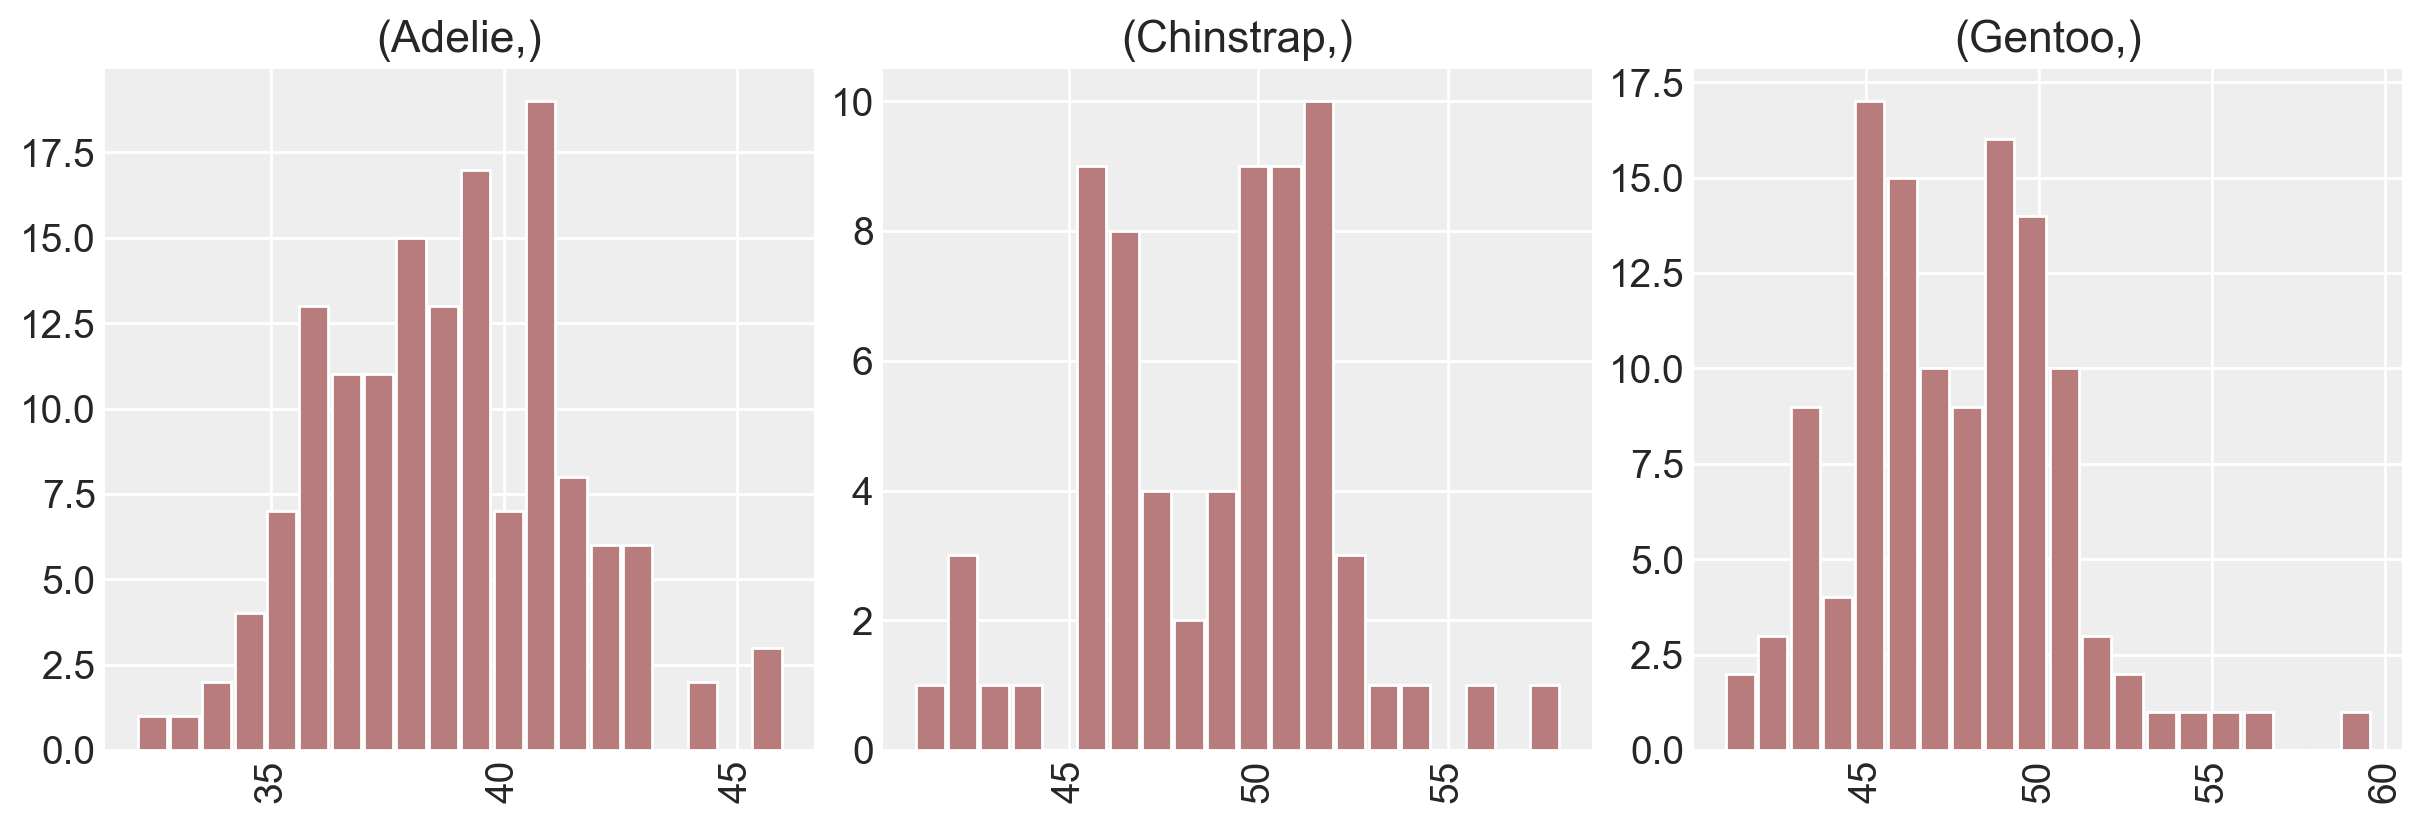
\includegraphics[width=12.61458in,height=4.28125in]{chapters/python/05_pandas_aggregate_files/figure-pdf/cell-13-output-1.png}

\begin{Shaded}
\begin{Highlighting}[]
\NormalTok{df}
\end{Highlighting}
\end{Shaded}

\begin{longtable}[]{@{}lllllllll@{}}
\toprule\noalign{}
& species & island & bill\_length\_mm & bill\_depth\_mm &
flipper\_length\_mm & body\_mass\_g & sex & year \\
\midrule\noalign{}
\endhead
\bottomrule\noalign{}
\endlastfoot
0 & Adelie & Torgersen & 39.1 & 18.7 & 181.0 & 3750.0 & male & 2007 \\
1 & Adelie & Torgersen & 39.5 & 17.4 & 186.0 & 3800.0 & female & 2007 \\
2 & Adelie & Torgersen & 40.3 & 18.0 & 195.0 & 3250.0 & female & 2007 \\
4 & Adelie & Torgersen & 36.7 & 19.3 & 193.0 & 3450.0 & female & 2007 \\
5 & Adelie & Torgersen & 39.3 & 20.6 & 190.0 & 3650.0 & male & 2007 \\
... & ... & ... & ... & ... & ... & ... & ... & ... \\
339 & Chinstrap & Dream & 55.8 & 19.8 & 207.0 & 4000.0 & male & 2009 \\
340 & Chinstrap & Dream & 43.5 & 18.1 & 202.0 & 3400.0 & female &
2009 \\
341 & Chinstrap & Dream & 49.6 & 18.2 & 193.0 & 3775.0 & male & 2009 \\
342 & Chinstrap & Dream & 50.8 & 19.0 & 210.0 & 4100.0 & male & 2009 \\
343 & Chinstrap & Dream & 50.2 & 18.7 & 198.0 & 3775.0 & female &
2009 \\
\end{longtable}

\subsection{Aggregazione dei dati}\label{aggregazione-dei-dati}

Il riepilogo di più valori in un unico indice va sotto il nome di
``aggregazione'' dei dati. Il metodo \texttt{aggregate()} può essere
applicato ai DataFrame e restituisce un nuovo DataFrame più breve
contenente solo i valori aggregati. Il primo argomento di
\texttt{aggregate()} specifica quale funzione o quali funzioni devono
essere utilizzate per aggregare i dati. Molte comuni funzioni di
aggregazione sono disponibili nel modulo \texttt{statistics}. Ad
esempio:

\begin{itemize}
\tightlist
\item
  \texttt{median()}: la mediana;
\item
  \texttt{mean()}: la media;
\item
  \texttt{stdev()}: la deviazione standard;
\end{itemize}

Se vogliamo applicare più funzioni di aggregazione, allora possiamo
raccogliere prima le funzioni in una lista e poi passare la lista ad
\texttt{aggregate()}.

\begin{Shaded}
\begin{Highlighting}[]
\CommentTok{\# Lista delle funzioni statistiche di riepilogo come stringhe}
\NormalTok{summary\_stats }\OperatorTok{=}\NormalTok{ [}\StringTok{"min"}\NormalTok{, }\StringTok{"median"}\NormalTok{, }\StringTok{"mean"}\NormalTok{, }\StringTok{"std"}\NormalTok{, }\StringTok{"max"}\NormalTok{]}

\CommentTok{\# Calcola le statistiche di riepilogo per le colonne numeriche usando aggregate}
\NormalTok{result }\OperatorTok{=}\NormalTok{ df[}
\NormalTok{    [}\StringTok{"bill\_length\_mm"}\NormalTok{, }\StringTok{"bill\_depth\_mm"}\NormalTok{, }\StringTok{"flipper\_length\_mm"}\NormalTok{, }\StringTok{"body\_mass\_g"}\NormalTok{]}
\NormalTok{].aggregate(summary\_stats)}

\BuiltInTok{print}\NormalTok{(result)}
\end{Highlighting}
\end{Shaded}

\begin{verbatim}
        bill_length_mm  bill_depth_mm  flipper_length_mm  body_mass_g
min          32.100000      13.100000         172.000000  2700.000000
median       44.500000      17.300000         197.000000  4050.000000
mean         43.992793      17.164865         200.966967  4207.057057
std           5.468668       1.969235          14.015765   805.215802
max          59.600000      21.500000         231.000000  6300.000000
\end{verbatim}

Si noti che Pandas ha applicato le funzioni di riepilogo a ogni colonna,
ma, per alcune colonne, le statistiche riassuntive non si possono
calcolare, ovvero tutte le colonne che contengono stringhe anziché
numeri. Di conseguenza, vediamo che alcuni dei risultati per tali
colonne sono contrassegnati con ``NaN''. Questa è un'abbreviazione di
``Not a Number'', talvolta utilizzata nell'analisi dei dati per
rappresentare valori mancanti o non definiti.

Molto spesso vogliamo calcolare le statistiche descrittive separatamente
per ciascun gruppo di osservazioni -- per esempio, nel caso presente,
potremmo volere distinguere le statistiche descrittive in base alla
specie dei pinguini. Questo risultato si ottiene con il metodo
\texttt{.groupby()}.

Il nome ``group by'' deriva da un comando nel linguaggio del database
SQL, ma forse è più semplice pensarlo nei termini coniati da Hadley
Wickham: split, apply, combine. Un esempio canonico di questa operazione
di split-apply-combine, in cui ``apply'' è un'aggregazione di
sommatoria, è illustrato nella figura seguente:

\begin{figure}

\centering{

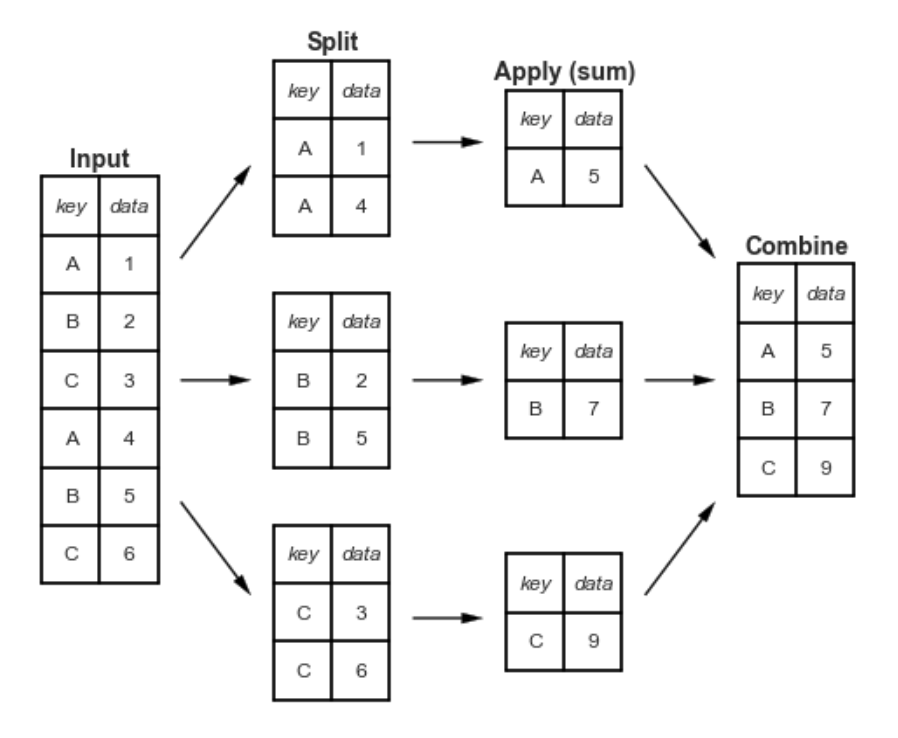
\includegraphics[width=0.7\textwidth,height=\textheight]{chapters/python/../../figures/split_apply_combine.png}

}

\caption{\label{fig-pandas}Split, apply, combine.}

\end{figure}%

La figura rende chiaro ciò che si ottiene con \texttt{groupby}:

\begin{itemize}
\tightlist
\item
  la fase ``split'' prevede la suddivisione e il raggruppamento di un
  DataFrame in base al valore della chiave specificata;
\item
  la fase ``apply'' implica il calcolo di alcune funzioni, solitamente
  un'aggregazione, una trasformazione o un filtro, all'interno dei
  singoli gruppi;
\item
  la fase ``combine'' unisce i risultati di queste operazioni in una
  matrice di output.
\end{itemize}

Per esempio, ragruppiamo le osservazioni \texttt{body\_mass\_g} in
funzione delle modalità della variabile \texttt{species}.

\begin{Shaded}
\begin{Highlighting}[]
\NormalTok{grouped }\OperatorTok{=}\NormalTok{ df[}\StringTok{"body\_mass\_g"}\NormalTok{].groupby(df[}\StringTok{"species"}\NormalTok{])}
\end{Highlighting}
\end{Shaded}

Calcoliamo ora la media della variabile \texttt{body\_mass\_g}
separatamente per ciascun gruppo di osservazioni.

\begin{Shaded}
\begin{Highlighting}[]
\NormalTok{grouped.mean()}
\end{Highlighting}
\end{Shaded}

\begin{verbatim}
species
Adelie       3706.164384
Chinstrap    3733.088235
Gentoo       5092.436975
Name: body_mass_g, dtype: float64
\end{verbatim}

È possibile applicare criteri di classificazione multipli. Per fare un
altro esempio, contiamo il numero di pinguini presenti sulle tre isole,
distinguendoli per specie e genere.

\begin{Shaded}
\begin{Highlighting}[]
\NormalTok{df.groupby([}\StringTok{"island"}\NormalTok{, }\StringTok{"species"}\NormalTok{, }\StringTok{"sex"}\NormalTok{]).size()}
\end{Highlighting}
\end{Shaded}

\begin{verbatim}
island     species    sex   
Biscoe     Adelie     female    22
                      male      22
           Gentoo     female    58
                      male      61
Dream      Adelie     female    27
                      male      28
           Chinstrap  female    34
                      male      34
Torgersen  Adelie     female    24
                      male      23
dtype: int64
\end{verbatim}

Con il metodo \texttt{aggregate()} possiamo applicare diverse funzioni
di aggregazione alle osservazioni ragruppate. Ad esempio

\begin{Shaded}
\begin{Highlighting}[]
\NormalTok{summary\_stats }\OperatorTok{=}\NormalTok{ [np.mean, np.std]}
\CommentTok{\# Group by "species" and calculate summary statistics for numeric columns}
\NormalTok{result }\OperatorTok{=}\NormalTok{ df.groupby(}\StringTok{"species"}\NormalTok{).agg(}
\NormalTok{    \{col: summary\_stats }\ControlFlowTok{for}\NormalTok{ col }\KeywordTok{in}\NormalTok{ df.columns }\ControlFlowTok{if}\NormalTok{ pd.api.types.is\_numeric\_dtype(df[col])\}}
\NormalTok{)}

\BuiltInTok{print}\NormalTok{(result)}
\end{Highlighting}
\end{Shaded}

\begin{verbatim}
          bill_length_mm           bill_depth_mm           flipper_length_mm  \
                    mean       std          mean       std              mean   
species                                                                        
Adelie         38.823973  2.662597     18.347260  1.219338        190.102740   
Chinstrap      48.833824  3.339256     18.420588  1.135395        195.823529   
Gentoo         47.568067  3.106116     14.996639  0.985998        217.235294   

                     body_mass_g                     year            
                std         mean         std         mean       std  
species                                                              
Adelie     6.521825  3706.164384  458.620135  2008.054795  0.811816  
Chinstrap  7.131894  3733.088235  384.335081  2007.970588  0.863360  
Gentoo     6.585431  5092.436975  501.476154  2008.067227  0.789025  
\end{verbatim}

Nella cella seguente troviamo la media di \texttt{body\_mass\_g} e
\texttt{flipper\_length\_mm} separatamente per ciascuna isola e ciascuna
specie:

\begin{Shaded}
\begin{Highlighting}[]
\NormalTok{df.groupby([}\StringTok{"island"}\NormalTok{, }\StringTok{"species"}\NormalTok{])[[}\StringTok{"body\_mass\_g"}\NormalTok{, }\StringTok{"flipper\_length\_mm"}\NormalTok{]].mean()}
\end{Highlighting}
\end{Shaded}

\begin{longtable}[]{@{}llll@{}}
\toprule\noalign{}
& & body\_mass\_g & flipper\_length\_mm \\
island & species & & \\
\midrule\noalign{}
\endhead
\bottomrule\noalign{}
\endlastfoot
\multirow{2}{=}{Biscoe} & Adelie & 3709.659091 & 188.795455 \\
& Gentoo & 5092.436975 & 217.235294 \\
\multirow{2}{=}{Dream} & Adelie & 3701.363636 & 189.927273 \\
& Chinstrap & 3733.088235 & 195.823529 \\
Torgersen & Adelie & 3708.510638 & 191.531915 \\
\end{longtable}

Facciamo la stessa cosa per la deviazione standard.

\begin{Shaded}
\begin{Highlighting}[]
\NormalTok{df.groupby([}\StringTok{"island"}\NormalTok{, }\StringTok{"species"}\NormalTok{])[[}\StringTok{"body\_mass\_g"}\NormalTok{, }\StringTok{"flipper\_length\_mm"}\NormalTok{]].std(ddof}\OperatorTok{=}\DecValTok{1}\NormalTok{)}
\end{Highlighting}
\end{Shaded}

\begin{longtable}[]{@{}llll@{}}
\toprule\noalign{}
& & body\_mass\_g & flipper\_length\_mm \\
island & species & & \\
\midrule\noalign{}
\endhead
\bottomrule\noalign{}
\endlastfoot
\multirow{2}{=}{Biscoe} & Adelie & 487.733722 & 6.729247 \\
& Gentoo & 501.476154 & 6.585431 \\
\multirow{2}{=}{Dream} & Adelie & 448.774519 & 6.480325 \\
& Chinstrap & 384.335081 & 7.131894 \\
Torgersen & Adelie & 451.846351 & 6.220062 \\
\end{longtable}

Prestiamo attenzione alla seguente sintassi:

\begin{Shaded}
\begin{Highlighting}[]
\NormalTok{summary\_stats }\OperatorTok{=}\NormalTok{ (}
\NormalTok{    df.loc[:, [}\StringTok{"island"}\NormalTok{, }\StringTok{"species"}\NormalTok{, }\StringTok{"body\_mass\_g"}\NormalTok{, }\StringTok{"flipper\_length\_mm"}\NormalTok{]]}
\NormalTok{    .groupby([}\StringTok{"island"}\NormalTok{, }\StringTok{"species"}\NormalTok{])}
\NormalTok{    .aggregate([}\StringTok{"mean"}\NormalTok{, }\StringTok{"std"}\NormalTok{, }\StringTok{"count"}\NormalTok{])}
\NormalTok{)}
\NormalTok{summary\_stats}
\end{Highlighting}
\end{Shaded}

\begin{longtable}[]{@{}llllllll@{}}
\toprule\noalign{}
& & \multicolumn{3}{l}{%
body\_mass\_g} & \multicolumn{3}{l@{}}{%
flipper\_length\_mm} \\
& & mean & std & count & mean & std & count \\
island & species & & & & & & \\
\midrule\noalign{}
\endhead
\bottomrule\noalign{}
\endlastfoot
\multirow{2}{=}{Biscoe} & Adelie & 3709.659091 & 487.733722 & 44 &
188.795455 & 6.729247 & 44 \\
& Gentoo & 5092.436975 & 501.476154 & 119 & 217.235294 & 6.585431 &
119 \\
\multirow{2}{=}{Dream} & Adelie & 3701.363636 & 448.774519 & 55 &
189.927273 & 6.480325 & 55 \\
& Chinstrap & 3733.088235 & 384.335081 & 68 & 195.823529 & 7.131894 &
68 \\
Torgersen & Adelie & 3708.510638 & 451.846351 & 47 & 191.531915 &
6.220062 & 47 \\
\end{longtable}

Nell'istruzione precedente selezioniamo tutte le righe (\texttt{:}) di
tre colonne di interesse:
\texttt{df.loc{[}:,\ {[}"island",\ "species",\ "body\_mass\_g",\ "flipper\_length\_mm"{]}{]}}.
L'istruzione \texttt{.groupby({[}"island",\ "species"{]})} ragruppa le
osservazioni (righe) secondo le modalità delle variabili \texttt{island}
e \texttt{species}. Infine
\texttt{.aggregate({[}"mean",\ "std",\ "count"{]})} applica i metodi
statistici specificati a ciascun gruppo di osservazioni. Con questa
sintassi la sequenza delle operazioni da eseguire diventa molto
intuitiva.

È possibile approfondire questo argomento consultanto il
\href{https://wesmckinney.com/book/data-aggregation.html}{capitolo 10}
del testo \emph{Python for Data Analysis} di McKinney (2022).

\section{Informazioni sull'Ambiente di
Sviluppo}\label{informazioni-sullambiente-di-sviluppo-4}

\begin{Shaded}
\begin{Highlighting}[]
\OperatorTok{\%}\NormalTok{load\_ext watermark}
\OperatorTok{\%}\NormalTok{watermark }\OperatorTok{{-}}\NormalTok{n }\OperatorTok{{-}}\NormalTok{u }\OperatorTok{{-}}\NormalTok{v }\OperatorTok{{-}}\NormalTok{iv }\OperatorTok{{-}}\NormalTok{w }\OperatorTok{{-}}\NormalTok{m}
\end{Highlighting}
\end{Shaded}

\begin{verbatim}
Last updated: Mon Jan 29 2024

Python implementation: CPython
Python version       : 3.11.7
IPython version      : 8.19.0

Compiler    : Clang 16.0.6 
OS          : Darwin
Release     : 23.3.0
Machine     : x86_64
Processor   : i386
CPU cores   : 8
Architecture: 64bit

scipy     : 1.11.4
seaborn   : 0.13.0
numpy     : 1.26.2
pandas    : 2.1.4
arviz     : 0.17.0
matplotlib: 3.8.2

Watermark: 2.4.3
\end{verbatim}

\chapter{Pandas (3)}\label{sec-pandas-3}

In questo tutorial, verranno presentate le funzioni di Pandas più utili
per condurre le usuali operazioni di manipolazione dei dati.

\begin{Shaded}
\begin{Highlighting}[]
\ImportTok{import}\NormalTok{ pandas }\ImportTok{as}\NormalTok{ pd}
\ImportTok{import}\NormalTok{ numpy }\ImportTok{as}\NormalTok{ np}
\ImportTok{import}\NormalTok{ matplotlib.pyplot }\ImportTok{as}\NormalTok{ plt}
\ImportTok{from}\NormalTok{ scipy }\ImportTok{import}\NormalTok{ stats}
\ImportTok{import}\NormalTok{ arviz }\ImportTok{as}\NormalTok{ az}
\ImportTok{import}\NormalTok{ seaborn }\ImportTok{as}\NormalTok{ sns}
\end{Highlighting}
\end{Shaded}

\begin{Shaded}
\begin{Highlighting}[]
\OperatorTok{\%}\NormalTok{config InlineBackend.figure\_format }\OperatorTok{=} \StringTok{\textquotesingle{}retina\textquotesingle{}}
\NormalTok{RANDOM\_SEED }\OperatorTok{=} \DecValTok{42}
\NormalTok{rng }\OperatorTok{=}\NormalTok{ np.random.default\_rng(RANDOM\_SEED)}
\NormalTok{az.style.use(}\StringTok{"arviz{-}darkgrid"}\NormalTok{)}
\NormalTok{sns.set\_theme(palette}\OperatorTok{=}\StringTok{"colorblind"}\NormalTok{)}
\end{Highlighting}
\end{Shaded}

Per questo tutorial, useremo nuovamente i dati \texttt{penguins.csv}.
Come in precedenza, dopo avere caricato i dati, rimuoviamo i dati
mancanti.

https://regenerativetoday.com/30-very-useful-pandas-functions-for-everyday-data-analysis-tasks/

\section{\texorpdfstring{\texttt{pd.read\_csv},
\texttt{pd.read\_excel}}{pd.read\_csv, pd.read\_excel}}\label{pd.read_csv-pd.read_excel}

La prima funzione da menzionare è \texttt{read\_csv} o
\texttt{read\_excel}. Le funzioni vengono utilizzate per leggere un file
CSV o un file Excel in formato DataFrame di Pandas. Qui stiamo
utilizzando la funzione \texttt{read\_csv} per leggere il dataset
\texttt{penguins}. In precedenza abbiamo anche visto come la funzione
\texttt{dropna} viene utilizzata per rimuovere tutte le righe del
DataFrame che includono dati mancanti.

\begin{Shaded}
\begin{Highlighting}[]
\NormalTok{df }\OperatorTok{=}\NormalTok{ pd.read\_csv(}\StringTok{"../data/penguins.csv"}\NormalTok{)}
\NormalTok{df.dropna(inplace}\OperatorTok{=}\VariableTok{True}\NormalTok{)}
\NormalTok{df.tail()}
\end{Highlighting}
\end{Shaded}

\begin{longtable}[]{@{}lllllllll@{}}
\toprule\noalign{}
& species & island & bill\_length\_mm & bill\_depth\_mm &
flipper\_length\_mm & body\_mass\_g & sex & year \\
\midrule\noalign{}
\endhead
\bottomrule\noalign{}
\endlastfoot
339 & Chinstrap & Dream & 55.8 & 19.8 & 207.0 & 4000.0 & male & 2009 \\
340 & Chinstrap & Dream & 43.5 & 18.1 & 202.0 & 3400.0 & female &
2009 \\
341 & Chinstrap & Dream & 49.6 & 18.2 & 193.0 & 3775.0 & male & 2009 \\
342 & Chinstrap & Dream & 50.8 & 19.0 & 210.0 & 4100.0 & male & 2009 \\
343 & Chinstrap & Dream & 50.2 & 18.7 & 198.0 & 3775.0 & female &
2009 \\
\end{longtable}

\section{\texorpdfstring{\texttt{.columns}}{.columns}}\label{columns}

Quando si dispone di un grande dataset, può essere difficile
visualizzare tutte le colonne. Utilizzando la funzione \texttt{columns},
è possibile stampare tutte le colonne del dataset.

\begin{Shaded}
\begin{Highlighting}[]
\NormalTok{df.columns}
\end{Highlighting}
\end{Shaded}

\begin{verbatim}
Index(['species', 'island', 'bill_length_mm', 'bill_depth_mm',
       'flipper_length_mm', 'body_mass_g', 'sex', 'year'],
      dtype='object')
\end{verbatim}

\section{\texorpdfstring{\texttt{.drop()}}{.drop()}}\label{drop}

È possibile eliminare alcune colonne non necessarie utilizzando
\texttt{drop}.

\begin{Shaded}
\begin{Highlighting}[]
\NormalTok{df }\OperatorTok{=}\NormalTok{ df.drop(columns}\OperatorTok{=}\NormalTok{[}\StringTok{"year"}\NormalTok{])}
\NormalTok{df.columns}
\end{Highlighting}
\end{Shaded}

\begin{verbatim}
Index(['species', 'island', 'bill_length_mm', 'bill_depth_mm',
       'flipper_length_mm', 'body_mass_g', 'sex'],
      dtype='object')
\end{verbatim}

\section{\texorpdfstring{\texttt{len()}}{len()}}\label{len}

Fornisce il numero di righe di un DataFrame.

\begin{Shaded}
\begin{Highlighting}[]
\BuiltInTok{len}\NormalTok{(df)}
\end{Highlighting}
\end{Shaded}

\begin{verbatim}
333
\end{verbatim}

\section{\texorpdfstring{\texttt{.query()}}{.query()}}\label{query}

È possibile filtrare un DataFrame utilizzando un'espressione booleana.

\begin{Shaded}
\begin{Highlighting}[]
\NormalTok{df1 }\OperatorTok{=}\NormalTok{ df.query(}\StringTok{"species == \textquotesingle{}Chinstrap\textquotesingle{} \& island == \textquotesingle{}Dream\textquotesingle{}"}\NormalTok{)}
\BuiltInTok{len}\NormalTok{(df1)}
\end{Highlighting}
\end{Shaded}

\begin{verbatim}
68
\end{verbatim}

\section{\texorpdfstring{\texttt{.iloc{[}{]}}}{.iloc{[}{]}}}\label{iloc}

Questa funzione accetta come parametri gli indici delle righe e delle
colonne, fornendo una selezione del DataFrame in base a questi. In
questo caso, stiamo selezionando le prime 3 righe di dati e le colonne
con indice 2, 3 e 5.

\begin{Shaded}
\begin{Highlighting}[]
\NormalTok{df2 }\OperatorTok{=}\NormalTok{ df.iloc[:}\DecValTok{3}\NormalTok{, [}\DecValTok{2}\NormalTok{, }\DecValTok{3}\NormalTok{, }\DecValTok{5}\NormalTok{]]}
\NormalTok{df2}
\end{Highlighting}
\end{Shaded}

\begin{longtable}[]{@{}llll@{}}
\toprule\noalign{}
& bill\_length\_mm & bill\_depth\_mm & body\_mass\_g \\
\midrule\noalign{}
\endhead
\bottomrule\noalign{}
\endlastfoot
0 & 39.1 & 18.7 & 3750.0 \\
1 & 39.5 & 17.4 & 3800.0 \\
2 & 40.3 & 18.0 & 3250.0 \\
\end{longtable}

\section{\texorpdfstring{\texttt{.loc{[}{]}}}{.loc{[}{]}}}\label{loc}

Questa funzione compie un'operazione molto simile a quella della
funzione \texttt{.iloc}. Tuttavia, in questo caso, abbiamo la
possibilità di specificare gli indici delle righe che desideriamo,
insieme ai nomi delle colonne che vogliamo includere nella nostra
selezione.

\begin{Shaded}
\begin{Highlighting}[]
\NormalTok{df3 }\OperatorTok{=}\NormalTok{ df.loc[[}\DecValTok{2}\NormalTok{, }\DecValTok{4}\NormalTok{, }\DecValTok{6}\NormalTok{], [}\StringTok{"island"}\NormalTok{, }\StringTok{"flipper\_length\_mm"}\NormalTok{, }\StringTok{"sex"}\NormalTok{]]}
\NormalTok{df3}
\end{Highlighting}
\end{Shaded}

\begin{longtable}[]{@{}llll@{}}
\toprule\noalign{}
& island & flipper\_length\_mm & sex \\
\midrule\noalign{}
\endhead
\bottomrule\noalign{}
\endlastfoot
2 & Torgersen & 195.0 & female \\
4 & Torgersen & 193.0 & female \\
6 & Torgersen & 181.0 & female \\
\end{longtable}

\section{Informazioni sull'Ambiente di
Sviluppo}\label{informazioni-sullambiente-di-sviluppo-5}

\begin{Shaded}
\begin{Highlighting}[]
\OperatorTok{\%}\NormalTok{load\_ext watermark}
\OperatorTok{\%}\NormalTok{watermark }\OperatorTok{{-}}\NormalTok{n }\OperatorTok{{-}}\NormalTok{u }\OperatorTok{{-}}\NormalTok{v }\OperatorTok{{-}}\NormalTok{iv }\OperatorTok{{-}}\NormalTok{w }\OperatorTok{{-}}\NormalTok{m}
\end{Highlighting}
\end{Shaded}

\begin{verbatim}
Last updated: Mon Jan 29 2024

Python implementation: CPython
Python version       : 3.11.7
IPython version      : 8.19.0

Compiler    : Clang 16.0.6 
OS          : Darwin
Release     : 23.3.0
Machine     : x86_64
Processor   : i386
CPU cores   : 8
Architecture: 64bit

seaborn   : 0.13.0
numpy     : 1.26.2
arviz     : 0.17.0
pandas    : 2.1.4
matplotlib: 3.8.2
scipy     : 1.11.4

Watermark: 2.4.3
\end{verbatim}

\chapter{Matplotlib}\label{sec-matplotlib}

Matplotlib è una libreria di visualizzazione in Python che permette di
creare una vasta gamma di figure statiche, animate e interattive.

\section{Preparazione del Notebook}\label{preparazione-del-notebook-2}

\begin{Shaded}
\begin{Highlighting}[]
\ImportTok{import}\NormalTok{ pandas }\ImportTok{as}\NormalTok{ pd}
\ImportTok{import}\NormalTok{ numpy }\ImportTok{as}\NormalTok{ np}
\ImportTok{import}\NormalTok{ matplotlib.pyplot }\ImportTok{as}\NormalTok{ plt}
\ImportTok{import}\NormalTok{ seaborn }\ImportTok{as}\NormalTok{ sns}
\ImportTok{import}\NormalTok{ arviz }\ImportTok{as}\NormalTok{ az}
\end{Highlighting}
\end{Shaded}

\begin{Shaded}
\begin{Highlighting}[]
\CommentTok{\# Questa istruzione consente di visualizzare i grafici generati dai comandi di }
\CommentTok{\# plot direttamente all\textquotesingle{}interno del notebook.}
\OperatorTok{\%}\NormalTok{config InlineBackend.figure\_format }\OperatorTok{=} \StringTok{\textquotesingle{}retina\textquotesingle{}}

\CommentTok{\# Questo valore viene usato come seed per il random number generator.}
\NormalTok{RANDOM\_SEED }\OperatorTok{=} \DecValTok{42}

\CommentTok{\# In questa riga, stai utilizzando il generatore di numeri casuali di NumPy per }
\CommentTok{\# creare una nuova istanza denominata rng. La funzione np.random.default\_rng() viene }
\CommentTok{\# utilizzata per inizializzare un generatore di numeri casuali con un seme specifico, }
\CommentTok{\# che in questo caso è RANDOM\_SEED.}
\NormalTok{rng }\OperatorTok{=}\NormalTok{ np.random.default\_rng(RANDOM\_SEED)}

\CommentTok{\# Queste due righe di codice sono spesso utilizzate per personalizzare l\textquotesingle{}aspetto dei }
\CommentTok{\# grafici in Python utilizzando le librerie ArviZ e Seaborn.}
\CommentTok{\# Questa riga di codice utilizza il metodo use() della libreria ArviZ per impostare uno }
\CommentTok{\# stile specifico per i tuoi grafici. In particolare, sta impostando lo stile chiamato }
\CommentTok{\# "arviz{-}darkgrid". Gli stili in ArviZ determinano come saranno visualizzati i grafici, inclusi colori, linee di griglia e altri dettagli estetici.}
\NormalTok{az.style.use(}\StringTok{"arviz{-}darkgrid"}\NormalTok{)}

\CommentTok{\# Questa riga di codice utilizza la libreria Seaborn per impostare il tema dei grafici. }
\CommentTok{\# In questo caso, il tema viene impostato utilizzando set\_theme() con il parametro palette }
\CommentTok{\# impostato su "colorblind". Questo significa che i colori utilizzati nei grafici saranno }
\CommentTok{\# scelti in modo da essere adatti alle persone con deficit visivi dei colori, rendendo i }
\CommentTok{\# grafici più accessibili.}
\NormalTok{sns.set\_theme(palette}\OperatorTok{=}\StringTok{"colorblind"}\NormalTok{)}
\end{Highlighting}
\end{Shaded}

\section{L'Interfaccia pyplot per Creare
Grafici}\label{linterfaccia-pyplot-per-creare-grafici}

Matplotlib è una libreria in Python famosa per la creazione di grafici,
e la sua interfaccia \texttt{pyplot} è particolarmente apprezzata per la
sua semplicità. Vediamo in dettaglio come funzionano le sue funzioni
principali. Per comprendere meglio come funzionano le sue funzioni
principali, possiamo fare un parallelo con il disegno su un supporto
fisico.

\begin{itemize}
\item
  \textbf{Prepariamo la Tela}: Iniziamo con \texttt{plt.figure()}, che è
  analogo a ottenere una tela bianca pronta per essere dipinta. È il
  punto di partenza, una superficie vuota su cui creeremo il nostro
  grafico.
\item
  \textbf{Definiamo le Aree di Disegno}: Successivamente, utilizzando
  \texttt{plt.subplot()} o \texttt{plt.axes()}, creiamo delle aree
  specifiche o ``assi'' sulla nostra tela. Questi assi corrispondono a
  diverse sezioni in cui posizioneremo vari elementi del nostro grafico,
  come se suddividessimo la tela fisica in diverse parti.
\item
  \textbf{Aggiungiamo Elementi al Grafico}: Una volta definiti gli assi,
  entriamo nel processo di creazione. Usandando funzioni come
  \texttt{plt.plot()} per tracciare linee o \texttt{plt.scatter()} per
  punti, aggiungiamo elementi grafici alla nostra area di disegno. È
  simile a disegnare direttamente sulla tela fisica.
\item
  \textbf{Rendiamo il Grafico Comprensibile}: Per garantire che il
  grafico sia chiaro e informativo, aggiungiamo etichette e titoli con
  \texttt{plt.xlabel()}, \texttt{plt.ylabel()} e \texttt{plt.title()}.
\end{itemize}

\section{Principi Fondamentali di
Pyplot}\label{principi-fondamentali-di-pyplot}

Esploriamo le funzionalità essenziali di \texttt{pyplot} di Matplotlib:

\begin{itemize}
\item
  \textbf{Creazione di Grafici Lineari}: Utilizzando
  \texttt{plt.plot(x,\ y)}, è possibile generare grafici lineari. Questa
  funzione necessita delle coordinate \texttt{x} e \texttt{y} per
  disegnare il grafico, semplificando così la rappresentazione visiva
  dei dati.
\item
  \textbf{Denominazione degli Assi}: È fondamentale assegnare
  un'etichetta appropriata agli assi per migliorare la comprensione del
  grafico. Si possono denominare gli assi tramite
  \texttt{plt.xlabel(\textquotesingle{}Nome\textquotesingle{})} per
  l'asse X e
  \texttt{plt.ylabel(\textquotesingle{}Nome\textquotesingle{})} per
  l'asse Y, facilitando l'interpretazione dei dati visualizzati.
\item
  \textbf{Inserimento del Titolo}: Un titolo descrittivo clarifica lo
  scopo o il contesto del grafico. Aggiungere un titolo è semplice con
  \texttt{plt.title(\textquotesingle{}Titolo\textquotesingle{})}, che
  aiuta a comunicare il messaggio principale del grafico in modo
  efficace.
\item
  \textbf{Inserimento di Legende}: Per grafici che includono più serie
  di dati o elementi distinti, l'aggiunta di una legenda è cruciale per
  la distinzione tra questi. La funzione \texttt{plt.legend()} permette
  di integrare una legenda, migliorando la leggibilità del grafico.
\item
  \textbf{Esposizione del Grafico}: Una volta completata la composizione
  del grafico, il passo finale è la sua visualizzazione. Attraverso
  \texttt{plt.show()}, è possibile mostrare il grafico elaborato,
  offrendo una visione complessiva dei dati analizzati.
\end{itemize}

\section{Esempio 1: Grafico lineare
semplice}\label{esempio-1-grafico-lineare-semplice}

\begin{Shaded}
\begin{Highlighting}[]
\NormalTok{x }\OperatorTok{=}\NormalTok{ [}\DecValTok{1}\NormalTok{, }\DecValTok{2}\NormalTok{, }\DecValTok{3}\NormalTok{, }\DecValTok{4}\NormalTok{]}
\NormalTok{y }\OperatorTok{=}\NormalTok{ [}\DecValTok{10}\NormalTok{, }\DecValTok{20}\NormalTok{, }\DecValTok{30}\NormalTok{, }\DecValTok{40}\NormalTok{]}

\NormalTok{plt.plot(x, y)}
\NormalTok{plt.xlabel(}\StringTok{"Asse X"}\NormalTok{)}
\NormalTok{plt.ylabel(}\StringTok{"Asse Y"}\NormalTok{)}
\NormalTok{plt.title(}\StringTok{"Grafico Lineare Semplice"}\NormalTok{)}\OperatorTok{;}
\end{Highlighting}
\end{Shaded}

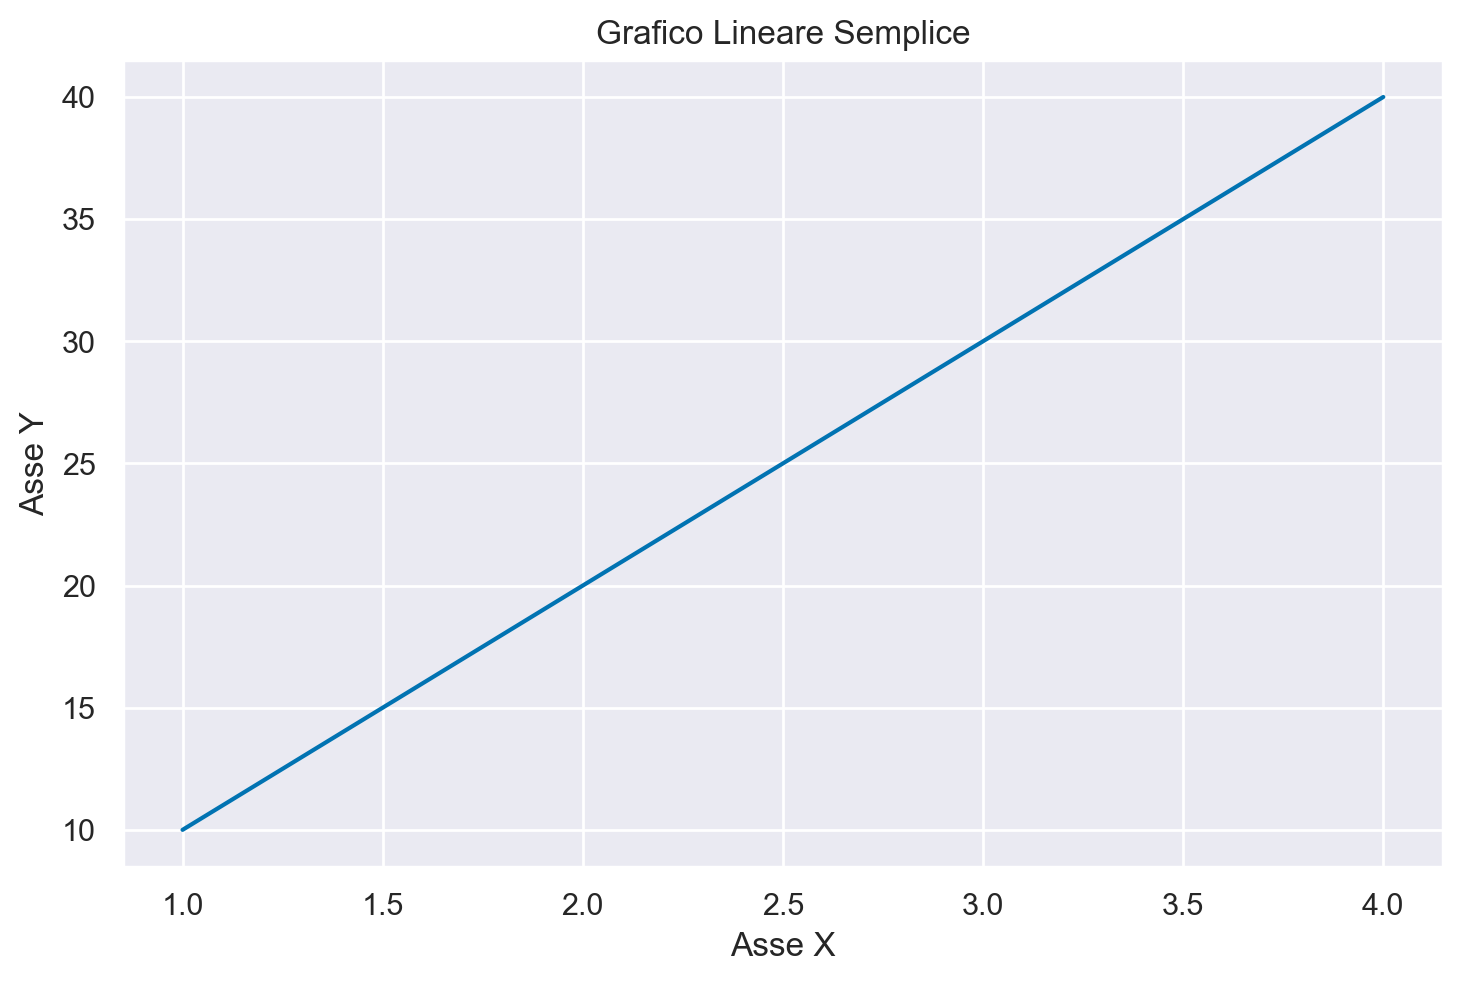
\includegraphics[width=7.61458in,height=5.11458in]{chapters/python/07_matplotlib_files/figure-pdf/cell-4-output-1.png}

\section{Esempio 2: Grafico con legenda e
stile}\label{esempio-2-grafico-con-legenda-e-stile}

\begin{Shaded}
\begin{Highlighting}[]
\NormalTok{x }\OperatorTok{=}\NormalTok{ [}\DecValTok{1}\NormalTok{, }\DecValTok{2}\NormalTok{, }\DecValTok{3}\NormalTok{, }\DecValTok{4}\NormalTok{]}
\NormalTok{y1 }\OperatorTok{=}\NormalTok{ [}\DecValTok{10}\NormalTok{, }\DecValTok{20}\NormalTok{, }\DecValTok{30}\NormalTok{, }\DecValTok{40}\NormalTok{]}
\NormalTok{y2 }\OperatorTok{=}\NormalTok{ [}\DecValTok{5}\NormalTok{, }\DecValTok{15}\NormalTok{, }\DecValTok{25}\NormalTok{, }\DecValTok{35}\NormalTok{]}

\NormalTok{plt.plot(x, y1, label}\OperatorTok{=}\StringTok{"Linea 1"}\NormalTok{, color}\OperatorTok{=}\StringTok{"C0"}\NormalTok{, linestyle}\OperatorTok{=}\StringTok{"{-}{-}"}\NormalTok{)}
\NormalTok{plt.plot(x, y2, label}\OperatorTok{=}\StringTok{"Linea 2"}\NormalTok{, color}\OperatorTok{=}\StringTok{"C3"}\NormalTok{, linestyle}\OperatorTok{=}\StringTok{"{-}"}\NormalTok{)}
\NormalTok{plt.xlabel(}\StringTok{"Asse X"}\NormalTok{)}
\NormalTok{plt.ylabel(}\StringTok{"Asse Y"}\NormalTok{)}
\NormalTok{plt.title(}\StringTok{"Grafico con Legenda"}\NormalTok{)}
\NormalTok{plt.legend()}\OperatorTok{;}
\end{Highlighting}
\end{Shaded}

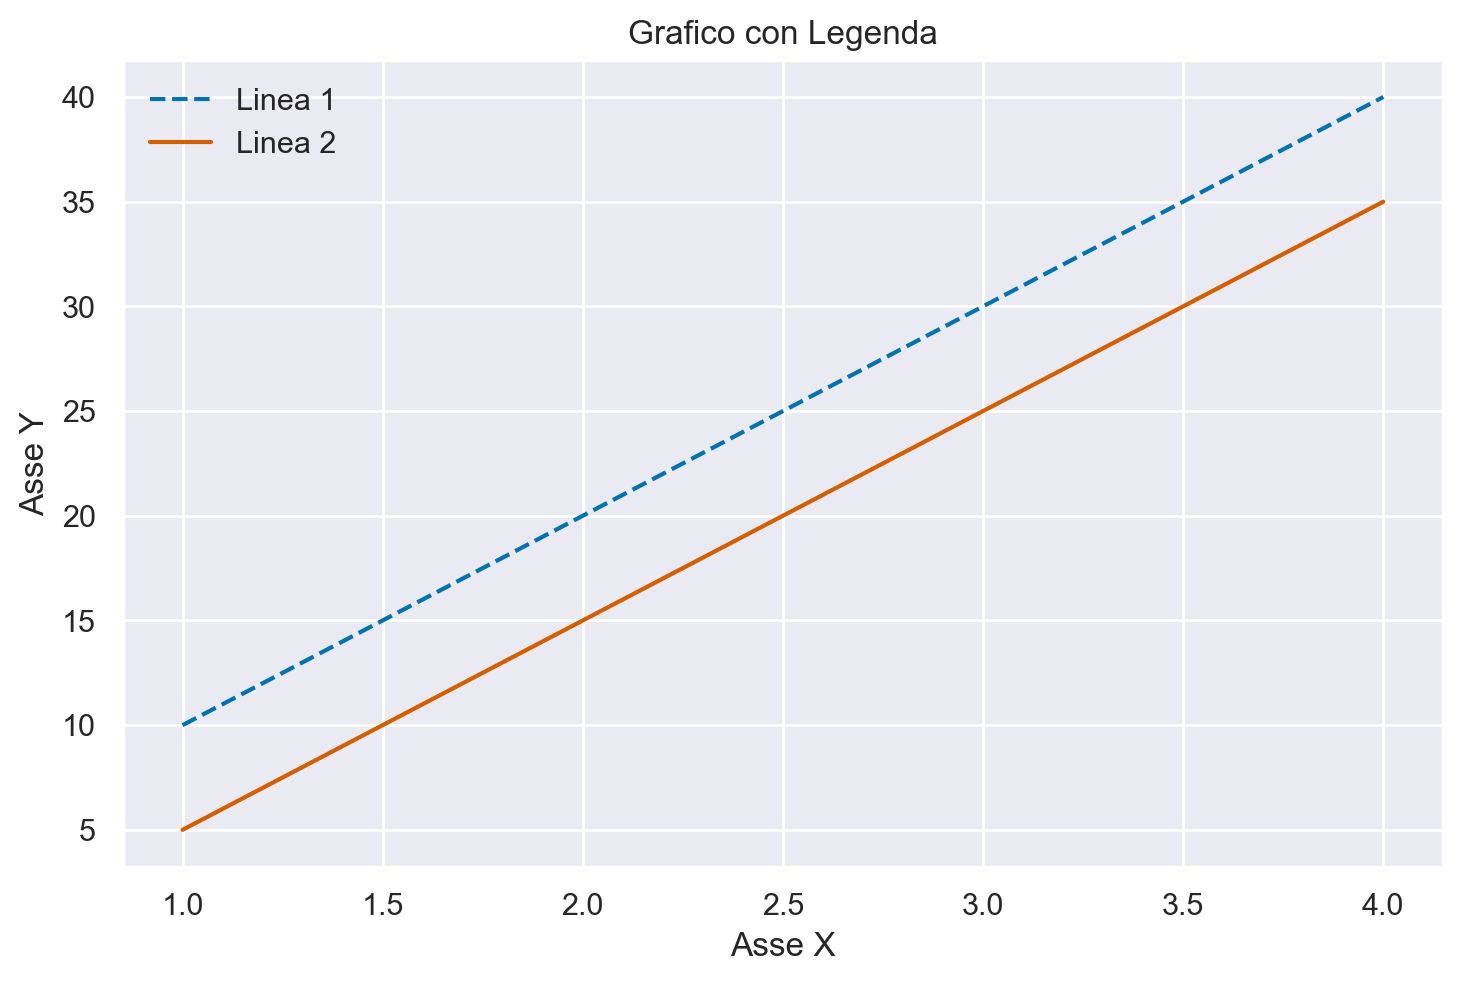
\includegraphics[width=7.61458in,height=5.11458in]{chapters/python/07_matplotlib_files/figure-pdf/cell-5-output-1.png}

\section{Esempio 3: Istogramma}\label{esempio-3-istogramma}

\begin{Shaded}
\begin{Highlighting}[]
\NormalTok{data }\OperatorTok{=}\NormalTok{ rng.normal(}\DecValTok{100}\NormalTok{, }\DecValTok{15}\NormalTok{, }\DecValTok{1000}\NormalTok{)}

\NormalTok{plt.hist(data, bins}\OperatorTok{=}\DecValTok{20}\NormalTok{)}
\NormalTok{plt.xlabel(}\StringTok{"Valori"}\NormalTok{)}
\NormalTok{plt.ylabel(}\StringTok{"Frequenza"}\NormalTok{)}
\NormalTok{plt.title(}\StringTok{"Istogramma"}\NormalTok{)}\OperatorTok{;}
\end{Highlighting}
\end{Shaded}

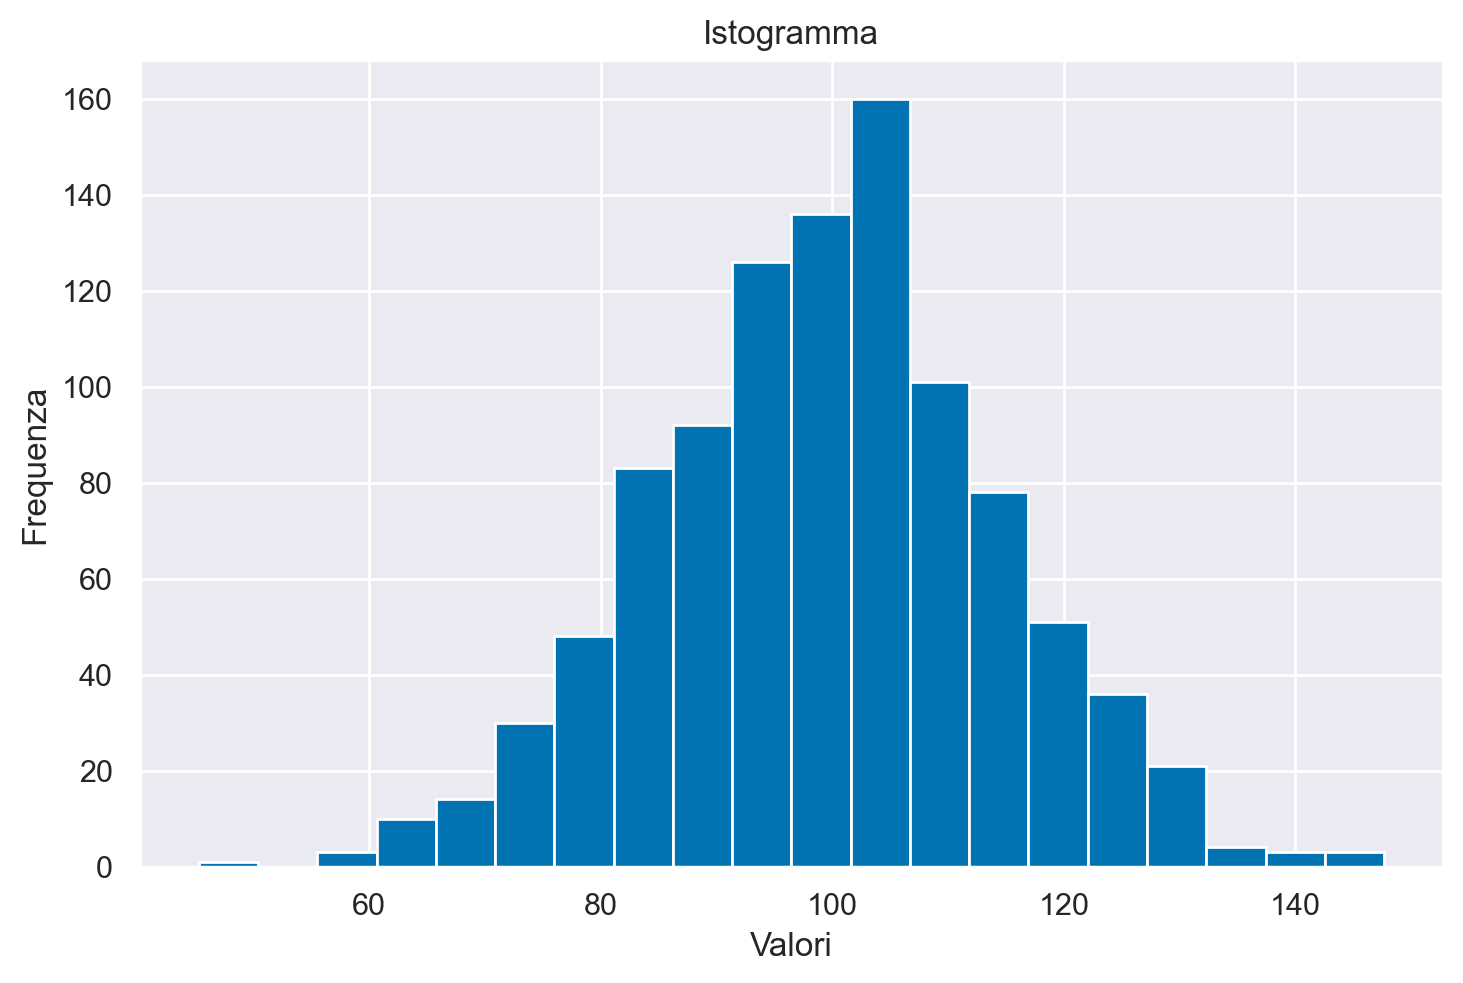
\includegraphics[width=7.61458in,height=5.11458in]{chapters/python/07_matplotlib_files/figure-pdf/cell-6-output-1.png}

\section{Esempio 4: pannelli
multipli}\label{esempio-4-pannelli-multipli}

Facciamo un altro esempio usando i dati \texttt{penguins.csv}.

\begin{Shaded}
\begin{Highlighting}[]
\NormalTok{df }\OperatorTok{=}\NormalTok{ pd.read\_csv(}\StringTok{"../data/penguins.csv"}\NormalTok{)}
\NormalTok{df.dropna(inplace}\OperatorTok{=}\VariableTok{True}\NormalTok{)}
\end{Highlighting}
\end{Shaded}

\begin{Shaded}
\begin{Highlighting}[]
\NormalTok{plt.figure(figsize}\OperatorTok{=}\NormalTok{(}\DecValTok{9}\NormalTok{, }\DecValTok{8}\NormalTok{))}

\NormalTok{plt.subplot(}\DecValTok{2}\NormalTok{, }\DecValTok{2}\NormalTok{, }\DecValTok{1}\NormalTok{)}
\NormalTok{plt.hist(df[}\StringTok{"bill\_depth\_mm"}\NormalTok{], }\DecValTok{10}\NormalTok{, density}\OperatorTok{=}\VariableTok{True}\NormalTok{, color}\OperatorTok{=}\StringTok{"C3"}\NormalTok{)}
\NormalTok{plt.title(}\StringTok{"Bill depth (mm)"}\NormalTok{)}\OperatorTok{;}

\NormalTok{plt.subplot(}\DecValTok{2}\NormalTok{, }\DecValTok{2}\NormalTok{, }\DecValTok{2}\NormalTok{)}
\NormalTok{sns.kdeplot(df[}\StringTok{"bill\_length\_mm"}\NormalTok{], fill}\OperatorTok{=}\VariableTok{True}\NormalTok{)}
\NormalTok{plt.title(}\StringTok{"KDE of Bill length (mm)"}\NormalTok{)}\OperatorTok{;}

\NormalTok{plt.subplot(}\DecValTok{2}\NormalTok{, }\DecValTok{2}\NormalTok{, }\DecValTok{3}\NormalTok{)}
\NormalTok{plt.scatter(x}\OperatorTok{=}\NormalTok{df[}\StringTok{"bill\_length\_mm"}\NormalTok{], y}\OperatorTok{=}\NormalTok{df[}\StringTok{"bill\_depth\_mm"}\NormalTok{], alpha}\OperatorTok{=}\FloatTok{0.4}\NormalTok{)}
\NormalTok{plt.title(}\StringTok{"Bill depth as a function of bill length"}\NormalTok{)}\OperatorTok{;}

\NormalTok{plt.subplot(}\DecValTok{2}\NormalTok{, }\DecValTok{2}\NormalTok{, }\DecValTok{4}\NormalTok{)}
\NormalTok{plt.boxplot(df[}\StringTok{"bill\_length\_mm"}\NormalTok{])}
\NormalTok{plt.title(}\StringTok{"Boxplot of Bill Length (mm)"}\NormalTok{)}

\NormalTok{plt.tight\_layout()}
\end{Highlighting}
\end{Shaded}

\begin{verbatim}
/var/folders/cl/wwjrsxdd5tz7y9jr82nd5hrw0000gn/T/ipykernel_55046/1324325854.py:19: UserWarning: The figure layout has changed to tight
  plt.tight_layout()
\end{verbatim}

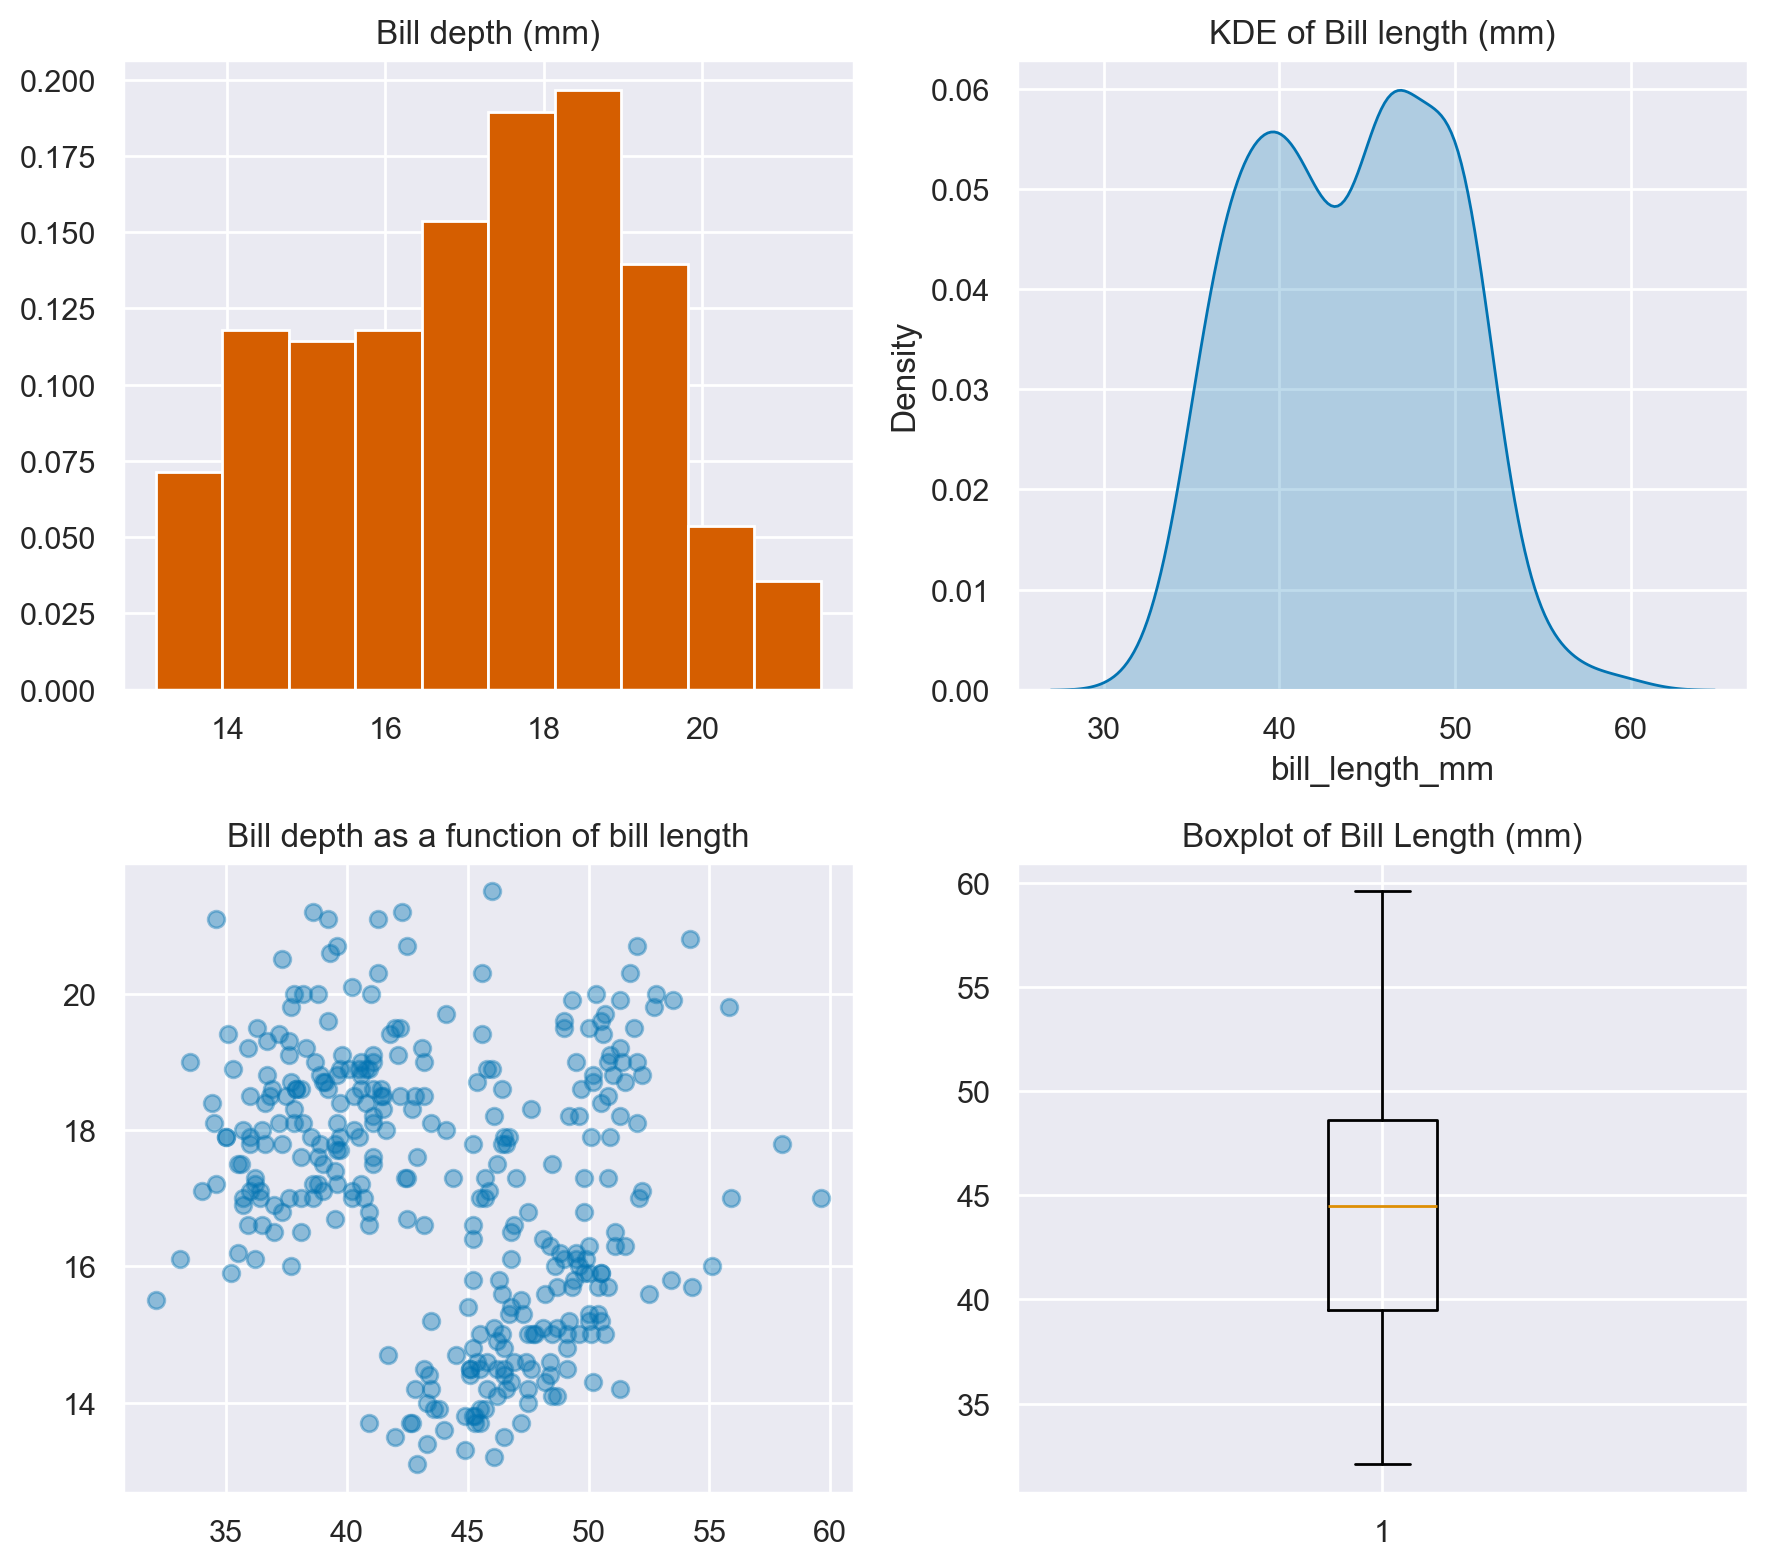
\includegraphics[width=9.19792in,height=8.15625in]{chapters/python/07_matplotlib_files/figure-pdf/cell-8-output-2.png}

Gli indici in \texttt{plt.subplot()} sono utilizzati per specificare
come dividere una figura in diverse aree di tracciamento, chiamate
``subplots''. La funzione \texttt{plt.subplot(nrows,\ ncols,\ index)}
prende tre argomenti principali:

\begin{itemize}
\tightlist
\item
  \texttt{nrows}: Numero di righe in cui la figura sarà suddivisa.
\item
  \texttt{ncols}: Numero di colonne in cui la figura sarà suddivisa.
\item
  \texttt{index}: Indice del subplot su cui operare, partendo
  dall'angolo in alto a sinistra e proseguendo da sinistra a destra e
  dall'alto in basso.
\end{itemize}

Nel codice precedente, \texttt{plt.subplot(2,\ 2,\ 1)} indica che la
figura sarà divisa in una griglia 2x2 (2 righe e 2 colonne) e che la
funzione \texttt{plt.hist()} agirà sul primo subplot, che si troverà
nell'angolo in alto a sinistra.

Gli altri indici (\texttt{2}, \texttt{3}, \texttt{4}) selezionano
rispettivamente il secondo subplot (in alto a destra), il terzo subplot
(in basso a sinistra) e il quarto subplot (in basso a destra) della
griglia 2x2.

Ecco come i subplot sono organizzati sulla figura:

\begin{verbatim}
+---------------------+----------------------+
|  plt.subplot(2,2,1) |  plt.subplot(2,2,2)  |
+---------------------+----------------------+
|  plt.subplot(2,2,3) |  plt.subplot(2,2,4)  |
+---------------------+----------------------+
\end{verbatim}

Ogni volta che si chiama \texttt{plt.subplot()} con un nuovo indice, il
``current axes'' cambia per puntare al subplot specificato. Quindi, le
funzioni di tracciamento come \texttt{plt.hist()},
\texttt{sns.kdeplot()}, \texttt{plt.scatter()} e \texttt{plt.boxplot()}
saranno applicate al subplot attualmente selezionato.

\section{Informazioni sull'Ambiente di
Sviluppo}\label{informazioni-sullambiente-di-sviluppo-6}

\begin{Shaded}
\begin{Highlighting}[]
\OperatorTok{\%}\NormalTok{load\_ext watermark}
\OperatorTok{\%}\NormalTok{watermark }\OperatorTok{{-}}\NormalTok{n }\OperatorTok{{-}}\NormalTok{u }\OperatorTok{{-}}\NormalTok{v }\OperatorTok{{-}}\NormalTok{iv }\OperatorTok{{-}}\NormalTok{w }\OperatorTok{{-}}\NormalTok{m}
\end{Highlighting}
\end{Shaded}

\begin{verbatim}
Last updated: Sat Feb 03 2024

Python implementation: CPython
Python version       : 3.11.7
IPython version      : 8.19.0

Compiler    : Clang 16.0.6 
OS          : Darwin
Release     : 23.3.0
Machine     : x86_64
Processor   : i386
CPU cores   : 8
Architecture: 64bit

numpy     : 1.26.2
arviz     : 0.17.0
matplotlib: 3.8.2
pandas    : 2.1.4
seaborn   : 0.13.0

Watermark: 2.4.3
\end{verbatim}

\chapter{Seaborn}\label{sec-seaborn}

\section{Elevare la Visualizzazione dei Dati con
Seaborn}\label{elevare-la-visualizzazione-dei-dati-con-seaborn}

Nel capitolo precedente, abbiamo esaminato Matplotlib, una libreria
estremamente versatile per la visualizzazione dei dati in Python. Ora
esamineremo le funzionalità di Seabonrn. Seaborn, che si basa su
Matplotlib, arricchisce l'esperienza di visualizzazione dei dati
offrendo una gamma più ampia e specializzata di opzioni grafiche,
particolarmente utili nel campo della data science.

Il vero punto di forza di Seaborn è la sua capacità di migliorare non
solo l'aspetto estetico dei grafici ma anche di facilitare la creazione
di visualizzazioni più complesse. Questo rende il processo più diretto e
intuitivo. La libreria è dotata di un'ampia varietà di strumenti, dalle
mappe di calore ai grafici a violino, permettendo agli utenti di
esplorare e rappresentare i dati in modi innovativi e informativi.

Per chi vuole approfondire ulteriormente, i tutorial presenti sul
\href{https://seaborn.pydata.org/}{sito ufficiale di Seaborn} sono una
risorsa preziosa e facilmente accessibile.

\section{Preparazione del Notebook}\label{preparazione-del-notebook-3}

\begin{Shaded}
\begin{Highlighting}[]
\ImportTok{import}\NormalTok{ pandas }\ImportTok{as}\NormalTok{ pd}
\ImportTok{import}\NormalTok{ numpy }\ImportTok{as}\NormalTok{ np}
\ImportTok{from}\NormalTok{ matplotlib }\ImportTok{import}\NormalTok{ pyplot }\ImportTok{as}\NormalTok{ plt}
\ImportTok{import}\NormalTok{ seaborn }\ImportTok{as}\NormalTok{ sns}
\ImportTok{import}\NormalTok{ arviz }\ImportTok{as}\NormalTok{ az}
\end{Highlighting}
\end{Shaded}

\begin{Shaded}
\begin{Highlighting}[]
\CommentTok{\# set seed to make the results fully reproducible}
\NormalTok{seed: }\BuiltInTok{int} \OperatorTok{=} \BuiltInTok{sum}\NormalTok{(}\BuiltInTok{map}\NormalTok{(}\BuiltInTok{ord}\NormalTok{, }\StringTok{"seaborn"}\NormalTok{))}
\NormalTok{rng: np.random.Generator }\OperatorTok{=}\NormalTok{ np.random.default\_rng(seed}\OperatorTok{=}\NormalTok{seed)}

\NormalTok{az.style.use(}\StringTok{"arviz{-}darkgrid"}\NormalTok{)}
\NormalTok{plt.rcParams[}\StringTok{"figure.dpi"}\NormalTok{] }\OperatorTok{=} \DecValTok{100}
\NormalTok{plt.rcParams[}\StringTok{"figure.facecolor"}\NormalTok{] }\OperatorTok{=} \StringTok{"white"}

\OperatorTok{\%}\NormalTok{config InlineBackend.figure\_format }\OperatorTok{=} \StringTok{"retina"}
\end{Highlighting}
\end{Shaded}

\section{Visualizzare la distribuzione dei
dati}\label{visualizzare-la-distribuzione-dei-dati}

Vediamo alcuni esempi pratici per scoprire come Seaborn possa
trasformare il modo in cui visualizziamo i dati.

Consideriamo nuovamente i dati Palmer penguin.

\begin{Shaded}
\begin{Highlighting}[]
\NormalTok{df }\OperatorTok{=}\NormalTok{ pd.read\_csv(}\StringTok{"../data/penguins.csv"}\NormalTok{)}
\end{Highlighting}
\end{Shaded}

Una delle forme di visualizzazione più comuni e informative nel campo
dell'analisi dei dati è l'istogramma, e la sua variante più sofisticata,
l'istogramma lisciato. Vediamo dunque come generare istogrammi che, per
il DataFrame \texttt{df}, sono stratificati sia in base alla specie che
al genere dei pinguini.

\begin{Shaded}
\begin{Highlighting}[]
\NormalTok{sns.displot(}
\NormalTok{    df, x}\OperatorTok{=}\StringTok{"flipper\_length\_mm"}\NormalTok{, col}\OperatorTok{=}\StringTok{"species"}\NormalTok{, row}\OperatorTok{=}\StringTok{"sex"}\NormalTok{,}
\NormalTok{    binwidth}\OperatorTok{=}\DecValTok{3}\NormalTok{, height}\OperatorTok{=}\DecValTok{3}\NormalTok{, facet\_kws}\OperatorTok{=}\BuiltInTok{dict}\NormalTok{(margin\_titles}\OperatorTok{=}\VariableTok{True}\NormalTok{),}
\NormalTok{)}\OperatorTok{;}
\end{Highlighting}
\end{Shaded}

Generiamo la stessa figura usando questa volta gli istogrammi lisciati.

\begin{Shaded}
\begin{Highlighting}[]
\NormalTok{sns.displot(}
\NormalTok{    df, x}\OperatorTok{=}\StringTok{"flipper\_length\_mm"}\NormalTok{, col}\OperatorTok{=}\StringTok{"species"}\NormalTok{, row}\OperatorTok{=}\StringTok{"sex"}\NormalTok{,}
\NormalTok{    height}\OperatorTok{=}\DecValTok{3}\NormalTok{, kind}\OperatorTok{=}\StringTok{"kde"}\NormalTok{, facet\_kws}\OperatorTok{=}\BuiltInTok{dict}\NormalTok{(margin\_titles}\OperatorTok{=}\VariableTok{True}\NormalTok{),}
\NormalTok{)}\OperatorTok{;}
\end{Highlighting}
\end{Shaded}

\begin{verbatim}
/opt/anaconda3/envs/pymc_env/lib/python3.12/site-packages/seaborn/axisgrid.py:123: UserWarning: The figure layout has changed to tight
  self._figure.tight_layout(*args, **kwargs)
\end{verbatim}

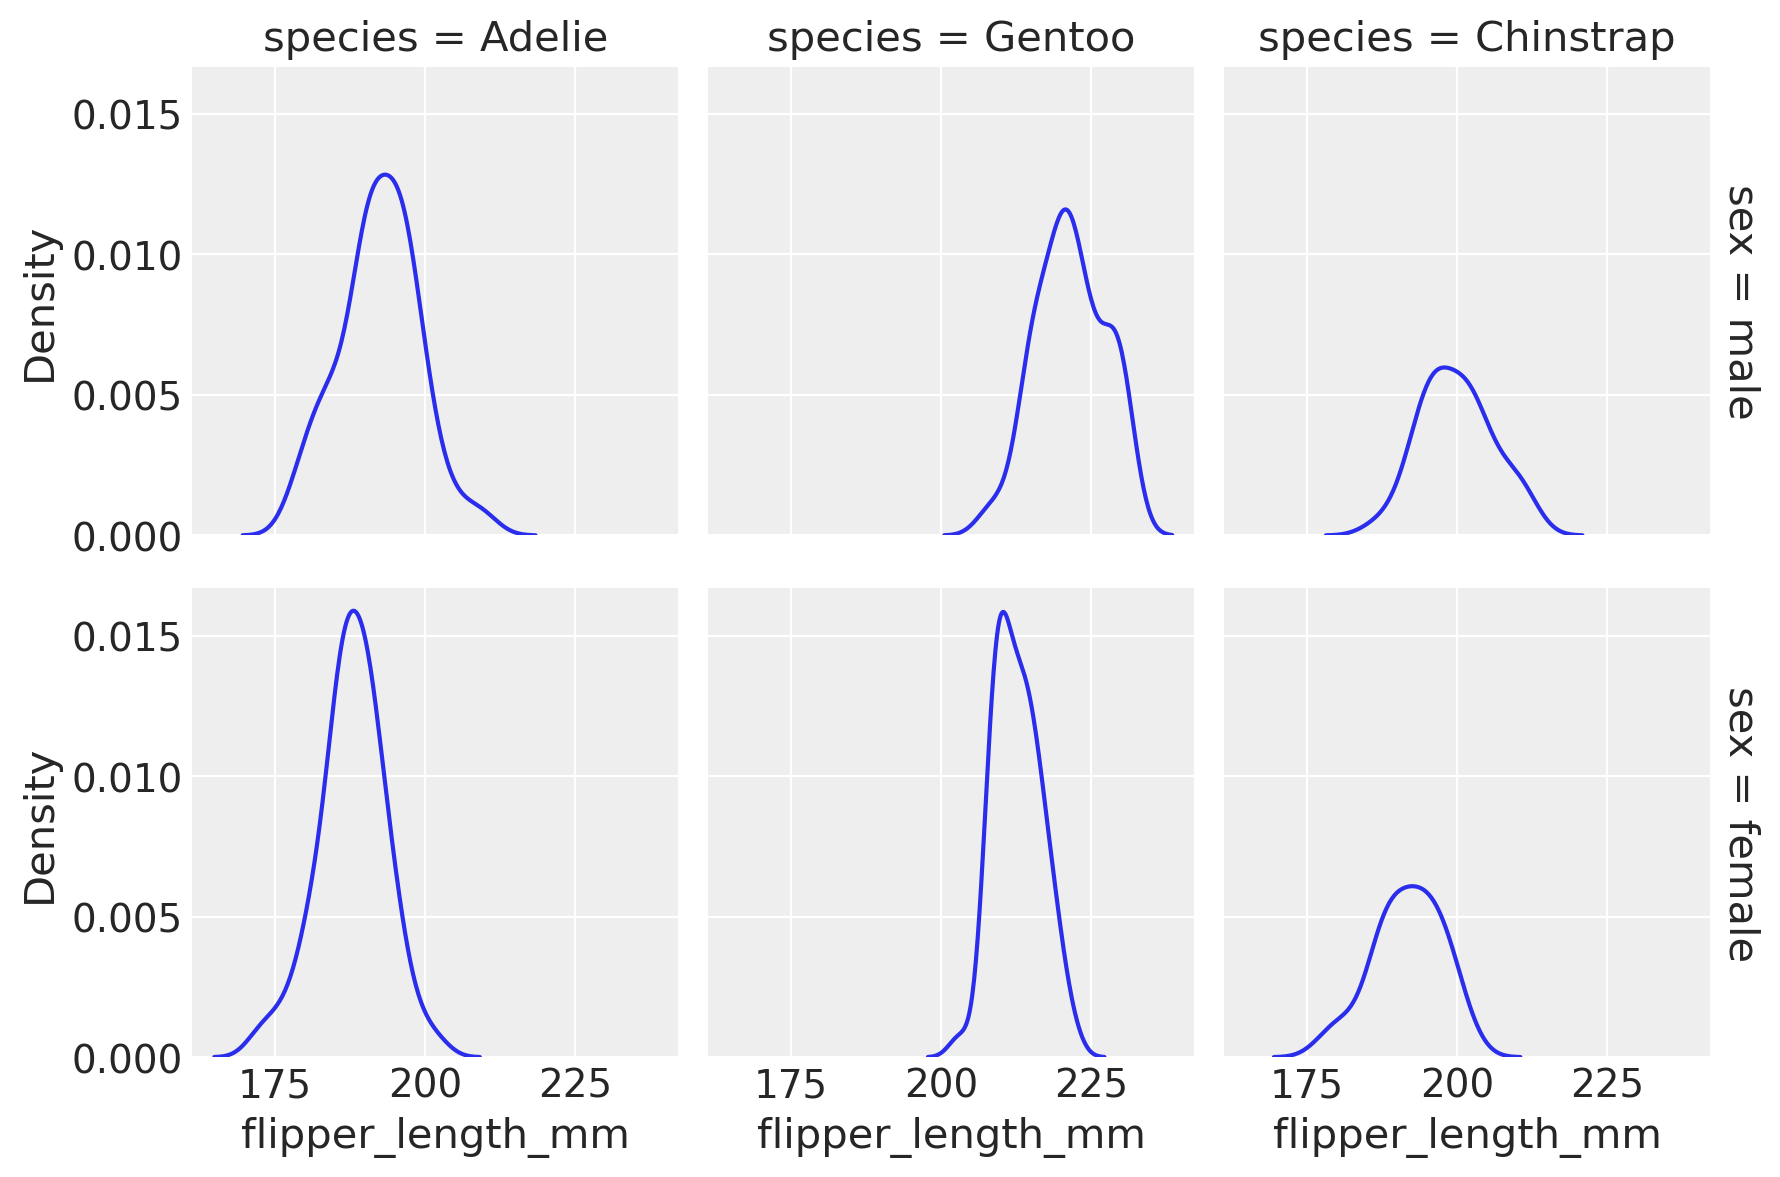
\includegraphics[width=9.27083in,height=6.125in]{chapters/python/08_seaborn_files/figure-pdf/cell-6-output-2.png}

\section{Visualizzazione di dati
categoriali}\label{visualizzazione-di-dati-categoriali}

Consideriamo ora il caso in cui si vuole rappresentare la relazione tra
una variabile numerica e una o più variabili categoriali.

Consideriamo, ad esempio, la massa corporea in relazione alla specie,
differenziando le osservazioni per genere. Creiamo il grafico
utilizzando i boxplot.

\begin{Shaded}
\begin{Highlighting}[]
\NormalTok{sns.catplot(df, x}\OperatorTok{=}\StringTok{"species"}\NormalTok{, y}\OperatorTok{=}\StringTok{"body\_mass\_g"}\NormalTok{, hue}\OperatorTok{=}\StringTok{"sex"}\NormalTok{, kind}\OperatorTok{=}\StringTok{"box"}\NormalTok{)}
\end{Highlighting}
\end{Shaded}

\begin{verbatim}
/opt/anaconda3/envs/pymc_env/lib/python3.12/site-packages/seaborn/axisgrid.py:123: UserWarning: The figure layout has changed to tight
  self._figure.tight_layout(*args, **kwargs)
\end{verbatim}

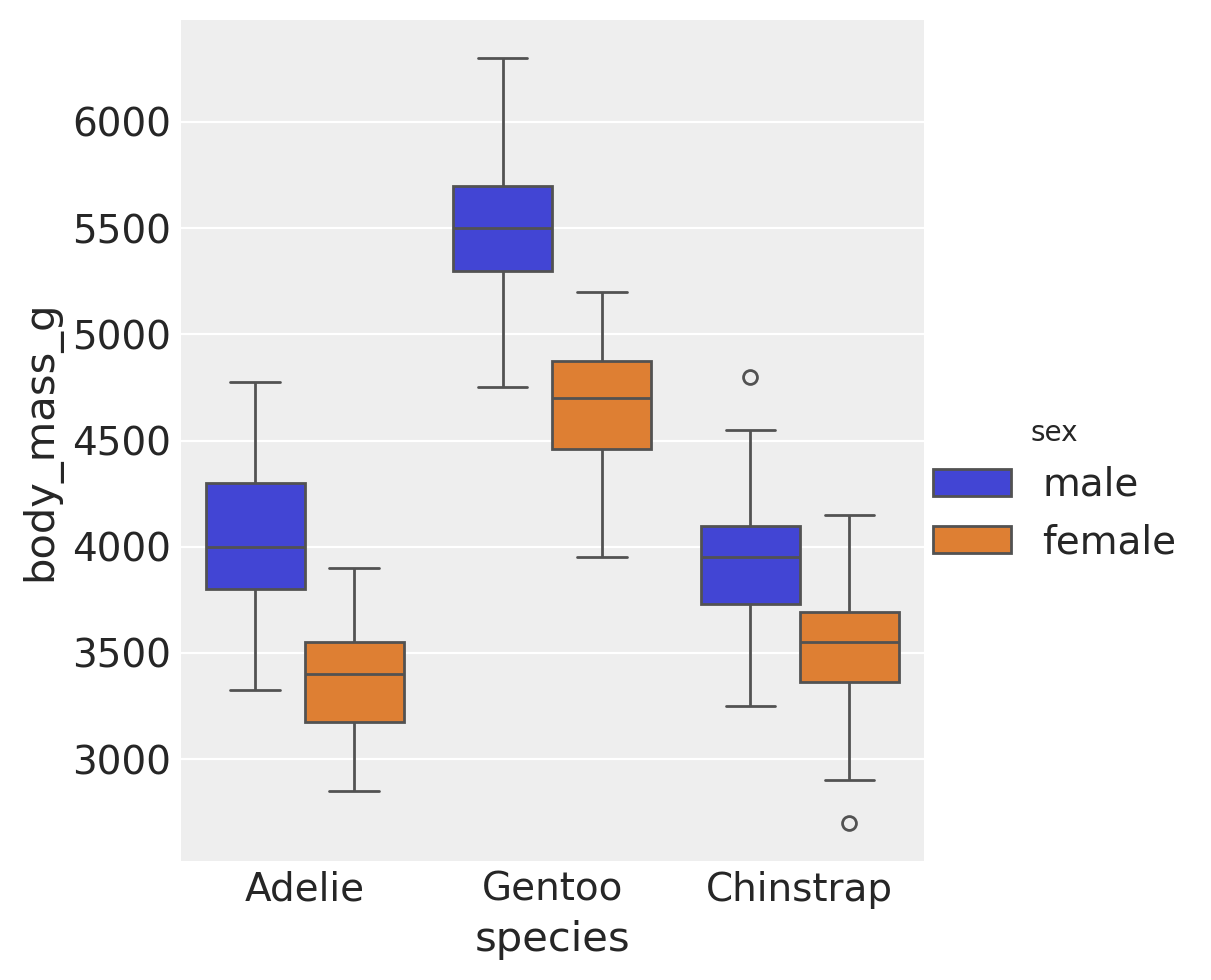
\includegraphics[width=6.30208in,height=5.10417in]{chapters/python/08_seaborn_files/figure-pdf/cell-7-output-2.png}

Dai diagrammi risulta evidente che i pinguini maschi hanno un peso
maggiore rispetto alle femmine in tutte le specie, e che i pinguini
Gentoo hanno un peso superiore rispetto ad Adelie e Chinstrap.

Come alternativa, possiamo utilizzare il violinplot per la
rappresentazione grafica dei dati.

\begin{Shaded}
\begin{Highlighting}[]
\NormalTok{sns.catplot(df, x}\OperatorTok{=}\StringTok{"species"}\NormalTok{, y}\OperatorTok{=}\StringTok{"body\_mass\_g"}\NormalTok{, hue}\OperatorTok{=}\StringTok{"sex"}\NormalTok{, kind}\OperatorTok{=}\StringTok{"violin"}\NormalTok{)}
\end{Highlighting}
\end{Shaded}

\begin{verbatim}
/opt/anaconda3/envs/pymc_env/lib/python3.12/site-packages/seaborn/axisgrid.py:123: UserWarning: The figure layout has changed to tight
  self._figure.tight_layout(*args, **kwargs)
\end{verbatim}

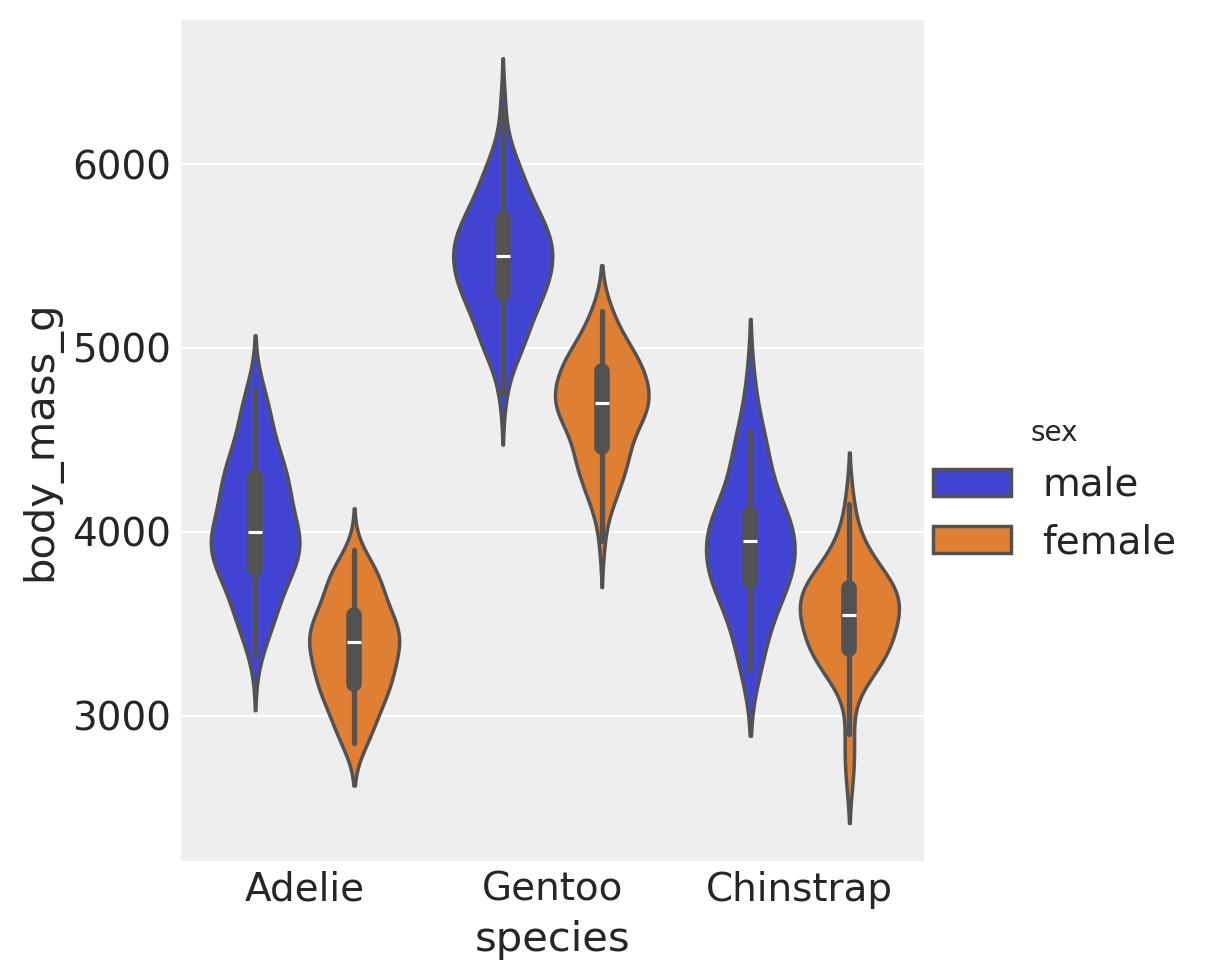
\includegraphics[width=6.30208in,height=5.10417in]{chapters/python/08_seaborn_files/figure-pdf/cell-8-output-2.png}

\section{Relazioni tra variabili}\label{relazioni-tra-variabili}

Calcoliamo la correlazione tra le variabili.

\begin{Shaded}
\begin{Highlighting}[]
\BuiltInTok{vars} \OperatorTok{=}\NormalTok{ [}\StringTok{"bill\_length\_mm"}\NormalTok{, }\StringTok{"bill\_depth\_mm"}\NormalTok{, }\StringTok{"flipper\_length\_mm"}\NormalTok{, }\StringTok{"body\_mass\_g"}\NormalTok{]}
\NormalTok{corr\_matrix }\OperatorTok{=}\NormalTok{ df[}\BuiltInTok{vars}\NormalTok{].corr().}\BuiltInTok{round}\NormalTok{(}\DecValTok{2}\NormalTok{)}
\NormalTok{corr\_matrix}
\end{Highlighting}
\end{Shaded}

\begin{longtable}[]{@{}lllll@{}}
\toprule\noalign{}
& bill\_length\_mm & bill\_depth\_mm & flipper\_length\_mm &
body\_mass\_g \\
\midrule\noalign{}
\endhead
\bottomrule\noalign{}
\endlastfoot
bill\_length\_mm & 1.00 & -0.24 & 0.66 & 0.60 \\
bill\_depth\_mm & -0.24 & 1.00 & -0.58 & -0.47 \\
flipper\_length\_mm & 0.66 & -0.58 & 1.00 & 0.87 \\
body\_mass\_g & 0.60 & -0.47 & 0.87 & 1.00 \\
\end{longtable}

Queste informazioni possono essere comunicate in forma più diretta se
usiamo una rappresentazione grafica.

\begin{Shaded}
\begin{Highlighting}[]
\NormalTok{sns.heatmap(corr\_matrix, annot}\OperatorTok{=}\VariableTok{True}\NormalTok{, linecolor}\OperatorTok{=}\StringTok{"white"}\NormalTok{, linewidths}\OperatorTok{=}\DecValTok{5}\NormalTok{)}\OperatorTok{;}
\end{Highlighting}
\end{Shaded}

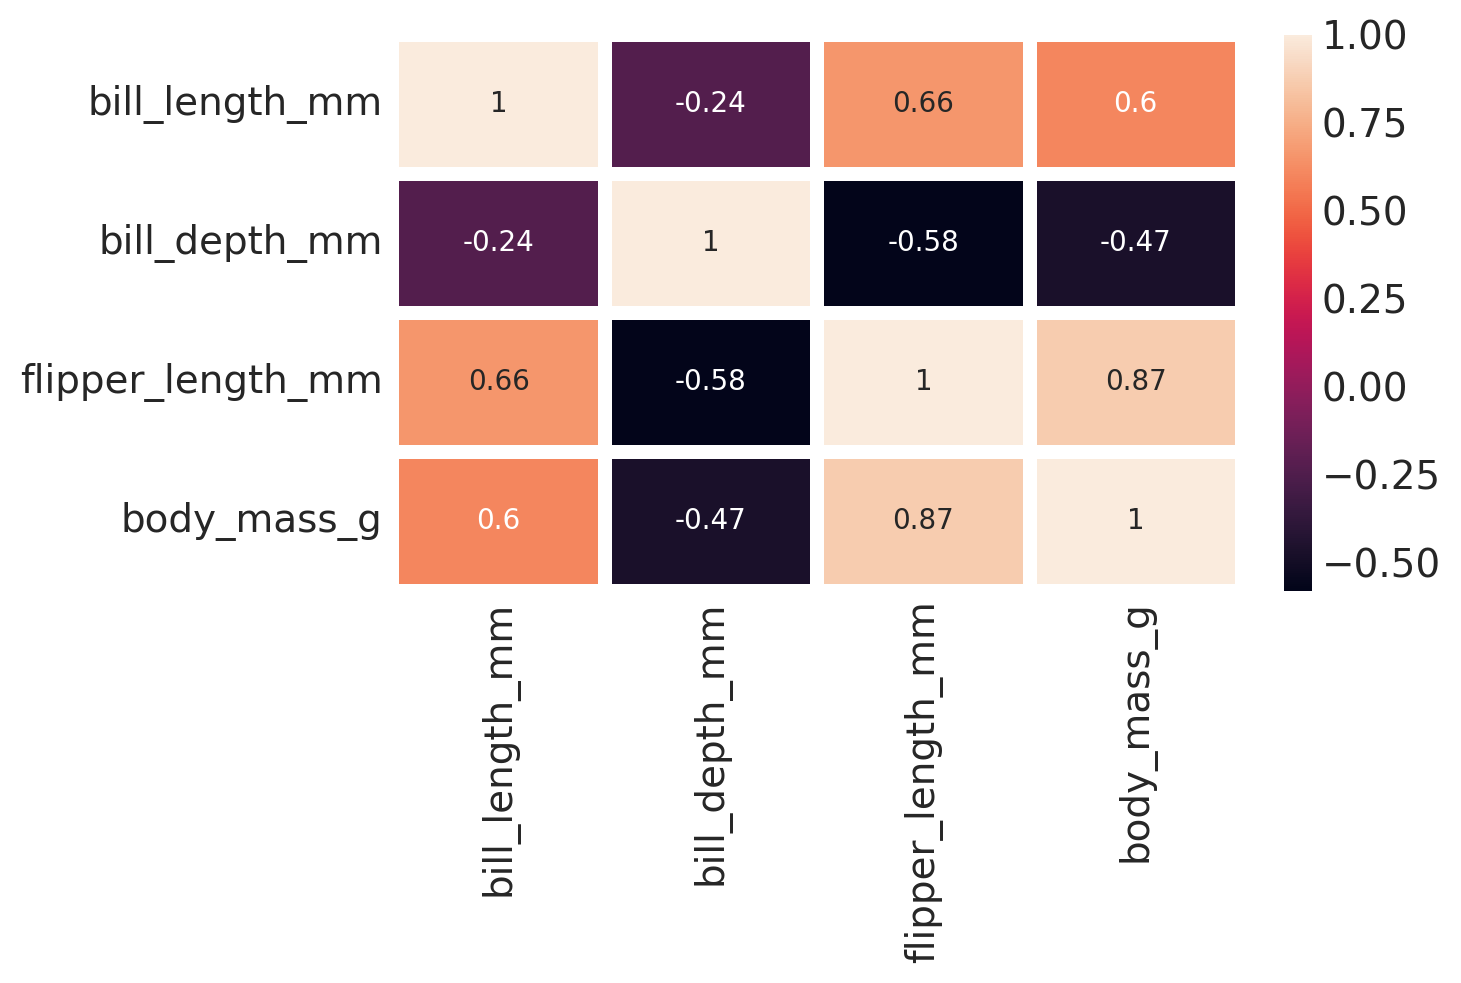
\includegraphics[width=7.60417in,height=5.11458in]{chapters/python/08_seaborn_files/figure-pdf/cell-10-output-1.png}

La lunghezza della pinna e la massa corporea mostrano un forte legame,
con una correlazione di 0.87. Ciò indica che i pinguini con pinne più
lunghe tendono a pesare di più.

Di seguito è riportato un esempio di diagramma a dispersione che
illustra questa relazione.

\begin{Shaded}
\begin{Highlighting}[]
\NormalTok{sns.scatterplot(df, x}\OperatorTok{=}\StringTok{"bill\_length\_mm"}\NormalTok{, y}\OperatorTok{=}\StringTok{"bill\_depth\_mm"}\NormalTok{, hue}\OperatorTok{=}\StringTok{"species"}\NormalTok{)}\OperatorTok{;}
\end{Highlighting}
\end{Shaded}

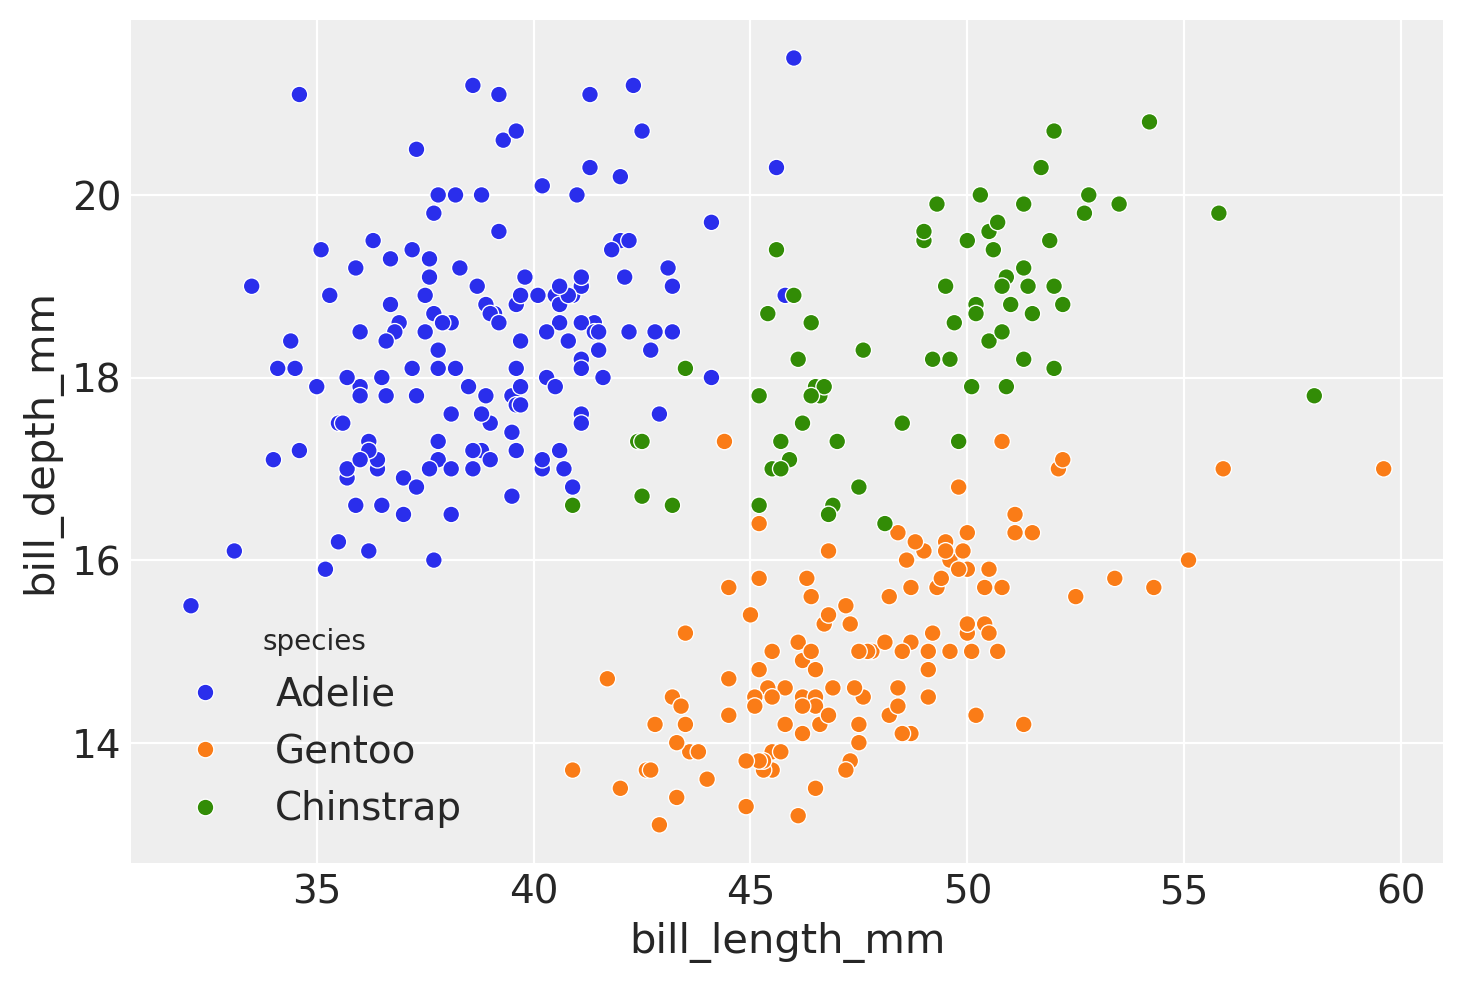
\includegraphics[width=7.61458in,height=5.11458in]{chapters/python/08_seaborn_files/figure-pdf/cell-11-output-1.png}

Evidentemente, le osservazioni delle tre specie formano cluster
distinti. Per ciascuna specie, la lunghezza e la larghezza del becco
presentano un intervallo specifico.

Spesso è vantaggioso creare grafici separati in base a diverse
dimensioni dei dati; nell'esempio seguente, suddividiamo i dati in base
all'isola di appartenenza.

\begin{Shaded}
\begin{Highlighting}[]
\NormalTok{g }\OperatorTok{=}\NormalTok{ sns.relplot(}
\NormalTok{    data}\OperatorTok{=}\NormalTok{df,}
\NormalTok{    x}\OperatorTok{=}\StringTok{"bill\_length\_mm"}\NormalTok{,}
\NormalTok{    y}\OperatorTok{=}\StringTok{"bill\_depth\_mm"}\NormalTok{,}
\NormalTok{    hue}\OperatorTok{=}\StringTok{"species"}\NormalTok{,}
\NormalTok{    row}\OperatorTok{=}\StringTok{"sex"}\NormalTok{,}
\NormalTok{    col}\OperatorTok{=}\StringTok{"island"}\NormalTok{,}
\NormalTok{    height}\OperatorTok{=}\DecValTok{3}\NormalTok{,}
\NormalTok{    facet\_kws}\OperatorTok{=}\BuiltInTok{dict}\NormalTok{(margin\_titles}\OperatorTok{=}\VariableTok{True}\NormalTok{),}
\NormalTok{)}
\NormalTok{g.set\_axis\_labels(}
    \StringTok{"Bill length (mm)"}\NormalTok{,}
    \StringTok{"Bill depth (mm)"}\NormalTok{,}
\NormalTok{)}\OperatorTok{;}
\end{Highlighting}
\end{Shaded}

\begin{verbatim}
/opt/anaconda3/envs/pymc_env/lib/python3.12/site-packages/seaborn/axisgrid.py:123: UserWarning: The figure layout has changed to tight
  self._figure.tight_layout(*args, **kwargs)
\end{verbatim}

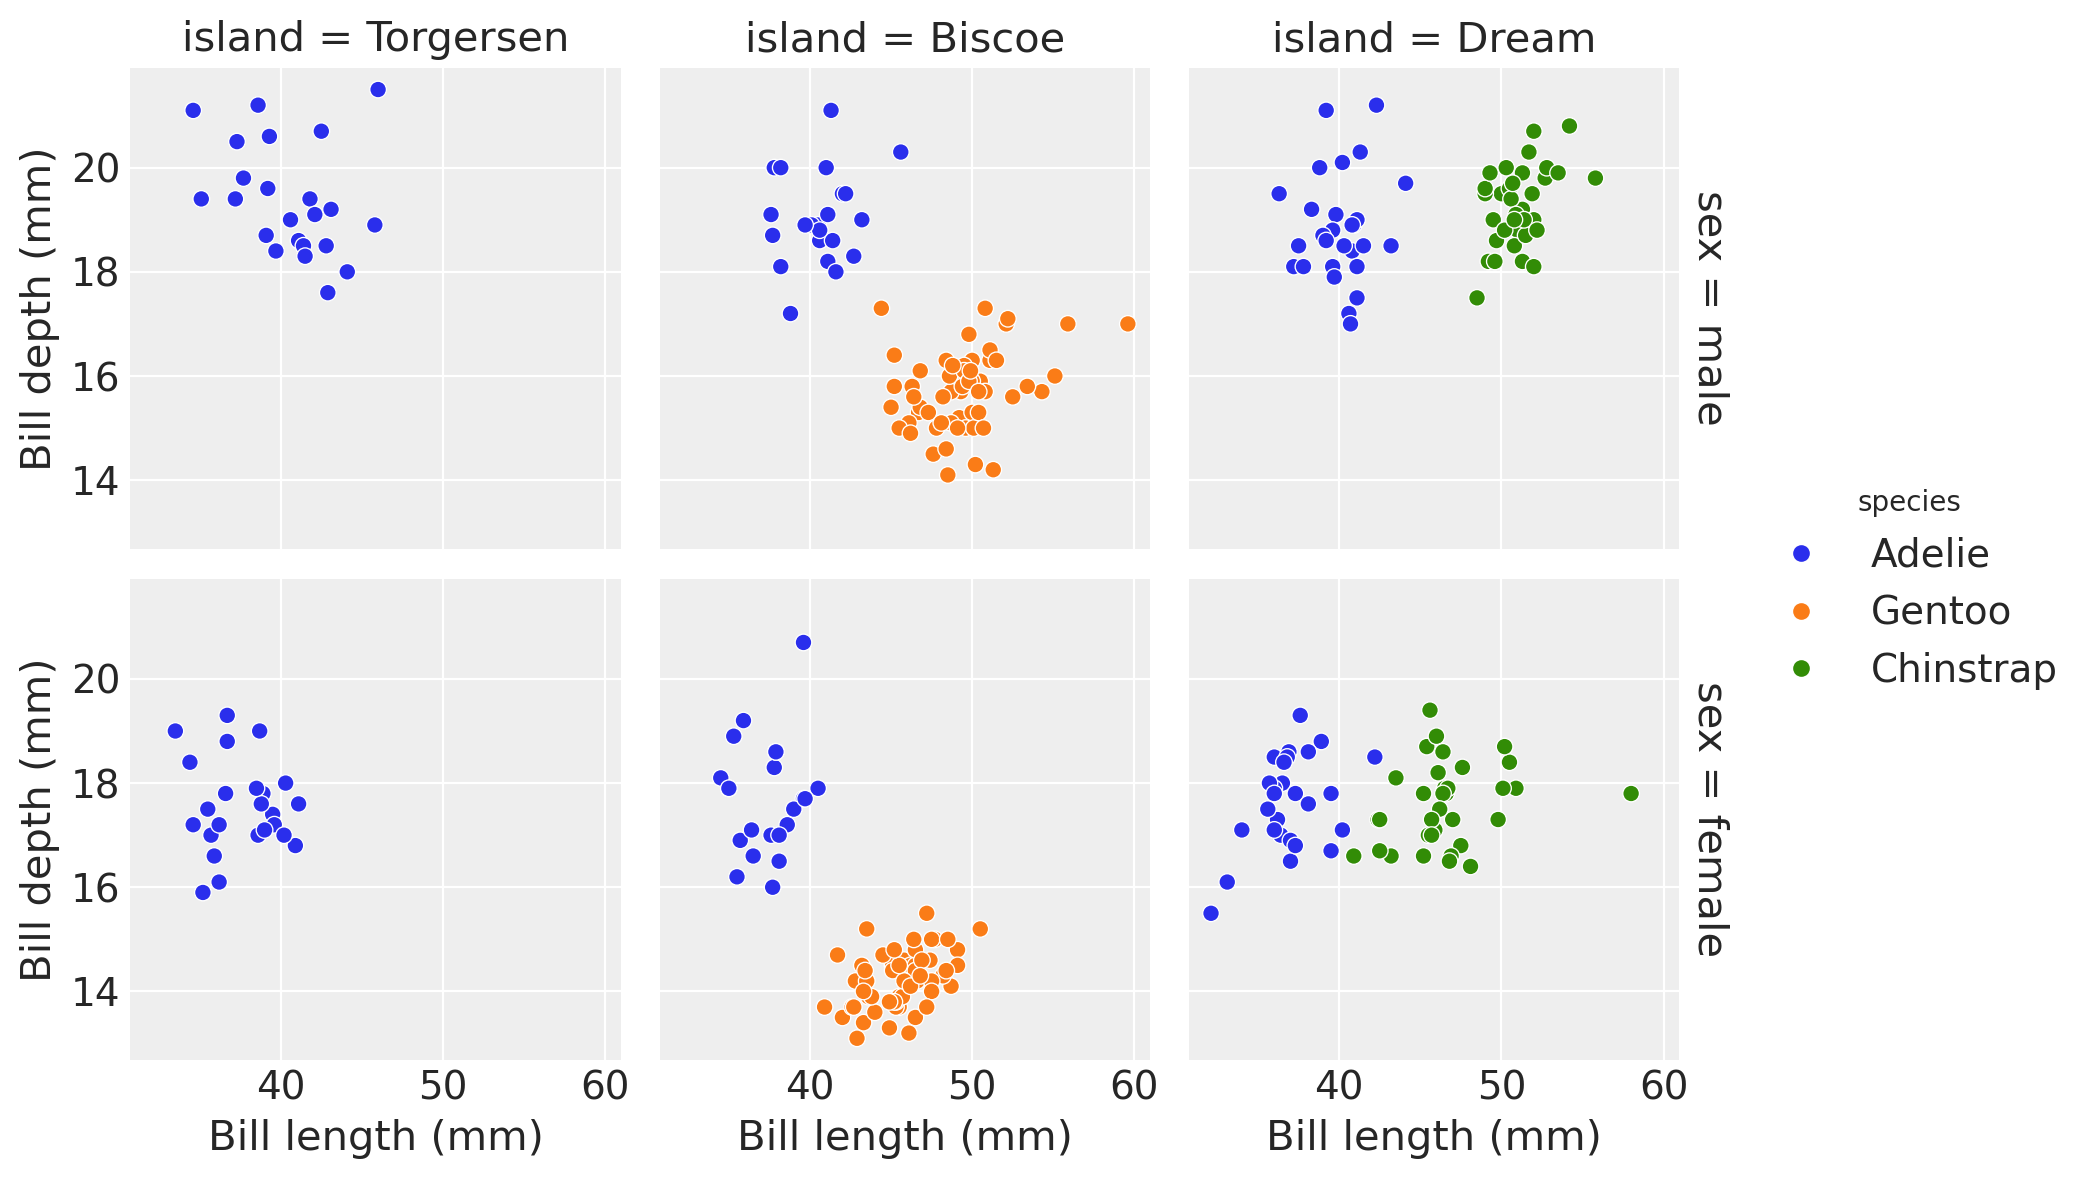
\includegraphics[width=10.89583in,height=6.13542in]{chapters/python/08_seaborn_files/figure-pdf/cell-12-output-2.png}

\section{Informazioni sull'Ambiente di
Sviluppo}\label{informazioni-sullambiente-di-sviluppo-7}

\begin{Shaded}
\begin{Highlighting}[]
\OperatorTok{\%}\NormalTok{load\_ext watermark}
\OperatorTok{\%}\NormalTok{watermark }\OperatorTok{{-}}\NormalTok{n }\OperatorTok{{-}}\NormalTok{u }\OperatorTok{{-}}\NormalTok{v }\OperatorTok{{-}}\NormalTok{iv }\OperatorTok{{-}}\NormalTok{w }\OperatorTok{{-}}\NormalTok{m}
\end{Highlighting}
\end{Shaded}

\begin{verbatim}
Last updated: Sat Jun 08 2024

Python implementation: CPython
Python version       : 3.12.3
IPython version      : 8.25.0

Compiler    : Clang 16.0.6 
OS          : Darwin
Release     : 23.4.0
Machine     : arm64
Processor   : arm
CPU cores   : 8
Architecture: 64bit

matplotlib: 3.8.4
arviz     : 0.18.0
pandas    : 2.2.2
numpy     : 1.26.4
seaborn   : 0.13.2

Watermark: 2.4.3
\end{verbatim}

\part{Fondamenti}

\chapter*{Introduzione}\label{introduzione-2}
\addcontentsline{toc}{chapter}{Introduzione}

\markboth{Introduzione}{Introduzione}

La data science è un campo che si sviluppa all'intersezione tra la
statistica e l'informatica. La statistica fornisce una serie di
metodologie per analizzare i dati e ottenere informazioni significative,
mentre l'informatica si occupa dello sviluppo di software e strumenti
per implementare tali metodologie. In questa sezione della dispensa,
approfondiremo alcuni concetti fondamentali della statistica e della
misurazione psicologica. Considereremo anche in termini generali quali
sono gli obiettivi e i limiti dell'analisi dei dati psicologici.

\chapter{Abbracciare l'incertezza}\label{sec-ucertainty}

\textbf{Prerequisiti}

\textbf{Concetti e competenze chiave}

\section{Introduzione}\label{introduzione-3}

L'espressione ``abbracciare l'incertezza'' è una delle frasi più
emblematiche tra i sostenitori della statistica bayesiana. In questo
capitolo esploreremo il significato di questa affermazione, basandoci
sulla trattazione presente nel primo capitolo di \emph{Understanding
uncertainty} di Lindley (2013). L'incertezza è un concetto centrale non
solo per la statistica, ma per qualsiasi disciplina scientifica, e in
particolare per la psicologia, che si confronta con fenomeni complessi e
difficili da misurare.

\section{L'incertezza nella ricerca
psicologica}\label{lincertezza-nella-ricerca-psicologica}

La psicologia, come molte altre scienze, si trova costantemente a
confrontarsi con l'incertezza. Che si tratti di indagare i processi
cognitivi, le emozioni o il comportamento umano, i ricercatori operano
in un contesto di dati complessi, spesso ambigui, e soggetti a
molteplici interpretazioni. Alcune affermazioni possono essere sostenute
con un alto grado di confidenza, altre smentite con decisione, ma la
maggior parte delle ipotesi cade in una zona grigia, in cui l'incertezza
regna sovrana.

Questo corso ha l'obiettivo di insegnare agli studenti come comprendere
e gestire l'incertezza nella ricerca psicologica, utilizzando
l'approccio bayesiano all'analisi dei dati. Questo metodo, incentrato
sulla quantificazione delle nostre credenze e sul loro aggiornamento in
base a nuove evidenze, permetterà agli studenti di affrontare in modo
rigoroso e sistematico l'incertezza nella loro carriera accademica e
nella pratica clinica.

\section{La natura soggettiva
dell'incertezza}\label{la-natura-soggettiva-dellincertezza}

Un aspetto fondamentale dell'incertezza, spesso trascurato, è la sua
dimensione soggettiva. Finetti (1970) ha sottolineato come l'incertezza
sia, in parte, una questione personale: ciò che è incerto per uno
psicologo può non esserlo per un altro, a seconda della loro esperienza,
conoscenza pregressa e interpretazione dei dati disponibili. Anche
quando due ricercatori condividono la stessa incertezza su un dato
problema, il loro grado di incertezza può variare notevolmente.

Questo elemento soggettivo è particolarmente rilevante in psicologia,
dove le differenze individuali e culturali influenzano la percezione e
l'interpretazione dei fenomeni. L'approccio bayesiano consente di
quantificare queste differenze soggettive, aggiornando le nostre
credenze in modo coerente sulla base delle informazioni oggettive e
della nostra esperienza.

\section{L'onnipresenza
dell'incertezza}\label{lonnipresenza-dellincertezza}

Nella ricerca psicologica, l'incertezza è onnipresente. Ogni
esperimento, ogni misurazione e ogni interpretazione dei dati comporta
un certo grado di incertezza. Questo è particolarmente vero quando si
studiano fenomeni complessi come il comportamento umano o i processi
mentali, influenzati da innumerevoli variabili, molte delle quali
difficili da controllare o misurare con precisione.

Nonostante ciò, l'incertezza non deve essere vista come un ostacolo
insormontabile. Al contrario, riconoscerla e quantificarla può portare a
una comprensione più profonda e realistica dei fenomeni psicologici.
Attraverso l'approccio bayesiano, impareremo a trattare l'incertezza
come una parte integrata del processo di indagine scientifica.

\section{Superare la soppressione
dell'incertezza}\label{superare-la-soppressione-dellincertezza}

Nonostante la sua onnipresenza, l'incertezza è spesso soppressa o
ignorata nella comunicazione scientifica. Questo avviene attraverso
interpretazioni eccessivamente ottimistiche dei risultati, presentazione
di conclusioni come fatti incontrovertibili o riluttanza nel riconoscere
i limiti degli studi condotti. Tale tendenza è comprensibile:
l'incertezza genera disagio, sia per i ricercatori che per il pubblico.
Tuttavia, ignorarla può portare a conclusioni errate e a una visione
distorta della realtà studiata.

L'approccio bayesiano permette di affrontare l'incertezza in modo
esplicito e costruttivo, insegnandoci a quantificarla, ragionarci sopra
e comunicarla chiaramente. Questo non solo migliora la trasparenza della
ricerca, ma consente di formulare conclusioni più accurate e oneste.

\section{I benefici dell'incertezza}\label{i-benefici-dellincertezza}

Contrariamente a quanto si possa pensare, l'incertezza offre numerosi
vantaggi alla ricerca psicologica:

\begin{itemize}
\tightlist
\item
  Stimola la curiosità e la ricerca: L'incertezza spinge i ricercatori a
  porre domande, esplorare nuove ipotesi e sviluppare metodi più
  raffinati per studiare i fenomeni psicologici.
\item
  Promuove l'onestà intellettuale: Riconoscere l'incertezza rende i
  ricercatori più cauti nelle loro affermazioni e aperti a prospettive
  alternative.
\item
  Migliora la qualità della ricerca: Considerare esplicitamente
  l'incertezza porta a disegni sperimentali più robusti e
  interpretazioni dei dati più accurate.
\item
  Facilita la collaborazione: Riconoscere i limiti della nostra
  conoscenza ci rende più propensi a cercare l'input di altri
  ricercatori e a collaborare in team interdisciplinari.
\item
  Riflette meglio la complessità della mente umana: L'incertezza è
  intrinseca a molti processi psicologici, e riconoscerla nei nostri
  modelli permette una rappresentazione più fedele di tale complessità.
\end{itemize}

\section{Tipi di incertezza}\label{tipi-di-incertezza}

Nella ricerca, l'incertezza riguarda la mancanza o insufficienza di
conoscenza. A seconda della sua origine, possiamo distinguere tra tre
principali tipi di incertezza: aleatoria, epistemica e ontologica
(Gansch e Adee 2020).

\subsection{Incertezza Aleatoria}\label{incertezza-aleatoria}

L'incertezza aleatoria deriva dalla natura intrinsecamente casuale di un
processo. È considerata irreducibile per un dato modello probabilistico
ed è quantificata tramite distribuzioni probabilistiche.

Ad esempio, se siamo interessati alla distribuzione delle posizioni di
due pianeti nello spazio, possiamo usare un modello probabilistico che
stima la probabilità che un pianeta si trovi in una determinata
posizione. Tuttavia, la posizione esatta è soggetta a incertezza
aleatoria.

\subsection{Incertezza Epistemica}\label{incertezza-epistemica}

L'incertezza epistemica riguarda la mancanza di conoscenza o la nostra
comprensione limitata di un fenomeno. Un elemento chiave è che siamo
consapevoli di questa mancanza: l'incertezza epistemica può essere
definita come il ``noto-ignoto'' di un modello.

Un modello è una rappresentazione semplificata della realtà, e questa
semplificazione introduce un'incertezza legata ai dettagli non inclusi.
Ad esempio, se iniziamo con un modello deterministico per il moto dei
pianeti, per masse puntiformi idealizzate, il modello è completamente
accurato e non ci sono incertezze. Tuttavia, nella realtà, i pianeti
possono avere una distribuzione di massa eterogenea, e un modello basato
su masse puntiformi non descrive più accuratamente il sistema fisico. La
mancanza di precisione nel modello porta a un'incertezza epistemica, che
potrebbe essere ridotta con un modello più accurato, ma richiederebbe
informazioni complete sulla distribuzione di massa, non sempre
disponibili.

Consideriamo ora un modello probabilistico: la distribuzione
probabilistica delle posizioni dei pianeti riflette l'incertezza
aleatoria, ma le probabilità stimate non sono sempre precise. Il divario
tra probabilità effettive e osservate rappresenta l'incertezza
epistemica del modello probabilistico.

\subsection{Incertezza Ontologica}\label{incertezza-ontologica}

L'incertezza ontologica si riferisce a una mancanza totale di conoscenza
su aspetti rilevanti di un sistema, descritta come ``ignoto-ignoto''.
Questo tipo di incertezza implica che vi siano fenomeni o variabili
sconosciuti che i nostri modelli non riescono ancora a identificare.

Tornando all'esempio dei pianeti, immaginiamo di modellare un sistema
con due pianeti. Se osserviamo comportamenti che non coincidono con le
previsioni del nostro modello, potrebbe esserci un terzo pianeta non
ancora scoperto che influisce sul sistema. Questa situazione rappresenta
un caso di incertezza ontologica, poiché si basa su fattori che non
avevamo preso in considerazione nel modello.

In sintesi, questi tre tipi di incertezza rappresentano differenti sfide
nella modellizzazione e nella comprensione dei sistemi complessi. Mentre
l'incertezza aleatoria è intrinseca e non può essere eliminata,
l'incertezza epistemica può essere ridotta migliorando i modelli e
ottenendo più informazioni. L'incertezza ontologica, invece, rappresenta
una frontiera di ciò che è ancora sconosciuto.

\section{Il calcolo bayesiano
dell'incertezza}\label{il-calcolo-bayesiano-dellincertezza}

Il nucleo di questo insegnamento sarà l'apprendimento di come
quantificare e ragionare sull'incertezza utilizzando l'approccio
bayesiano (Gelman et al. 1995). Basato sul teorema di Bayes, questo
metodo fornisce un framework coerente per aggiornare le credenze alla
luce di nuove evidenze.

I passi fondamentali includono:

\begin{enumerate}
\def\labelenumi{\arabic{enumi}.}
\tightlist
\item
  Quantificare le credenze iniziali (prior) su fenomeni psicologici.
\item
  Valutare la forza dell'evidenza fornita dai dati (likelihood).
\item
  Combinare prior e likelihood per ottenere credenze aggiornate
  (posterior).
\item
  Usare queste credenze aggiornate per prendere decisioni e pianificare
  ulteriori ricerche.
\end{enumerate}

Questo approccio trasforma l'incertezza in una quantità con cui
ragionare rigorosamente e matematicamente.

\section{Credenze e decisioni nella ricerca
psicologica}\label{credenze-e-decisioni-nella-ricerca-psicologica}

Le credenze guidano le decisioni dei ricercatori, che possono riguardare
il disegno di esperimenti, l'interpretazione dei risultati o la scelta
di interventi clinici. L'approccio bayesiano fornisce strumenti per:

\begin{itemize}
\tightlist
\item
  Articolare chiaramente le credenze prima di condurre una ricerca.
\item
  Aggiornare le credenze man mano che si raccolgono nuovi dati.
\item
  Prendere decisioni ottimali basate sulle credenze aggiornate.
\item
  Comunicare in modo trasparente l'incertezza associata alle
  conclusioni.
\end{itemize}

L'adozione di un approccio bayesiano può contribuire a una psicologia
più affidabile, capace di affrontare le sfide complesse del tentativo di
comprendere la mente e il comportamento umano.

\section{Conclusione}\label{conclusione}

Questo insegnamento guiderà verso l'analisi bayesiana dei dati
psicologici, insegnando a riconoscere l'incertezza come parte integrante
del processo scientifico. Utilizzando l'incertezza come strumento,
possiamo ottenere una comprensione più sfumata e profonda dei fenomeni
psicologici.

\chapter{Concetti chiave}\label{sec-key-notions}

\textbf{Prerequisiti}

\begin{itemize}
\tightlist
\item
  Leggere \href{../../figures/horoscopes.pdf}{Horoscopes}. L'ultimo
  capitolo di McElreath (2020) discute il contesto scientifico e
  culturale della statistica.
\item
  Leggere \href{https://theeffectbook.net}{The Effect: An Introduction
  to Research Design and Causality}. Focalizzati sul capitolo 10
  \emph{Treatment Effects}.
\end{itemize}

\textbf{Concetti e competenze chiave}

\begin{itemize}
\tightlist
\item
  Definizione di popolazione e campione.
\item
  Distinzione tra variabili indipendenti e dipendenti.
\item
  La matrice dei dati.
\item
  L'effetto delle variabili all'interno dell'analisi statistica.
\item
  I concetti di stima e inferenza.
\item
  Il concetto di modello psicologico.
\end{itemize}

\textbf{Preparazione del Notebook}

\begin{Shaded}
\begin{Highlighting}[]
\ImportTok{import}\NormalTok{ numpy }\ImportTok{as}\NormalTok{ np}
\ImportTok{import}\NormalTok{ pandas }\ImportTok{as}\NormalTok{ pd}
\end{Highlighting}
\end{Shaded}

\section*{Introduzione}\label{introduzione-4}
\addcontentsline{toc}{section}{Introduzione}

\markright{Introduzione}

\begin{quote}
Most of the fundamental ideas of science are essentially simple, and
may, as a rule, be expressed in a language comprehensible to everyone.\\
(Einstein A and Infeld L, 1938)
\end{quote}

L'\href{https://imstat.org/2014/09/04/data-science-how-is-it-different-to-statistics\%E2\%80\%89/}{analisi
dei dati} si colloca all'intersezione tra statistica, teoria della
probabilità e informatica. Questa disciplina multidisciplinare richiede
una solida comprensione dei concetti fondamentali provenienti da
ciascuna di queste tre aree.

\begin{itemize}
\item
  \textbf{Statistica.} La statistica fornisce gli strumenti e le
  tecniche per raccogliere, analizzare e interpretare i dati. Attraverso
  metodi descrittivi e inferenziali, permette di trarre conclusioni dai
  dati e di prendere decisioni informate. La statistica fornisce gli
  strumenti e le tecniche per raccogliere, analizzare e interpretare i
  dati. Attraverso metodi descrittivi e inferenziali, la statistica
  permette di trarre conclusioni dai dati e di prendere decisioni
  informate.
\item
  \textbf{Teoria della probabilità.} La teoria della probabilità
  costituisce la base matematica della statistica, modellando
  l'incertezza e comprendendo i fenomeni aleatori, fornendo i fondamenti
  per sviluppare metodi statistici rigorosi.
\item
  \textbf{Informatica.} L'informatica gioca un ruolo cruciale
  nell'analisi dei dati, offrendo gli strumenti necessari per la
  gestione, l'elaborazione e la visualizzazione dei dati su larga scala.
  Conoscere i principi dell'informatica è essenziale per sfruttare
  appieno tecnologie moderne come il machine learning e l'intelligenza
  artificiale. L'uso di linguaggi di programmazione come Python e R,
  insieme a librerie specializzate, permette di eseguire analisi
  complesse e di visualizzare i dati in modo efficace.
\end{itemize}

\begin{tcolorbox}[enhanced jigsaw, opacityback=0, breakable, left=2mm, opacitybacktitle=0.6, coltitle=black, rightrule=.15mm, colbacktitle=quarto-callout-note-color!10!white, colframe=quarto-callout-note-color-frame, toprule=.15mm, bottomtitle=1mm, toptitle=1mm, leftrule=.75mm, titlerule=0mm, title=\textcolor{quarto-callout-note-color}{\faInfo}\hspace{0.5em}{Statistica}, arc=.35mm, bottomrule=.15mm, colback=white]

Il termine ``statistica'' può assumere diversi significati, a seconda
del contesto in cui viene utilizzato.

\begin{itemize}
\tightlist
\item
  Nel primo senso, la statistica è una scienza e una disciplina che si
  occupa dello studio e dell'applicazione di metodi e tecniche per la
  raccolta, l'organizzazione, l'analisi, l'interpretazione e la
  presentazione di dati.
\item
  Nel secondo senso, il termine ``statistica'' si riferisce a una
  singola misura o un valore numerico che è stato calcolato a partire da
  un campione di dati. Questo tipo di statistica rappresenta una
  caratteristica specifica del campione. Esempi comuni di statistiche in
  questo senso includono la media campionaria, la deviazione standard
  campionaria o il coefficiente di correlazione campionario.
\end{itemize}

\end{tcolorbox}

\section{Popolazioni e Campioni}\label{popolazioni-e-campioni}

Per iniziare l'analisi dei dati, è fondamentale individuare le unità che
contengono le informazioni rilevanti per il fenomeno di interesse.
Questo insieme di unità costituisce la popolazione o universo,
rappresentando l'insieme completo di entità capaci di fornire
informazioni per l'indagine statistica in questione. Le singole unità
dell'insieme sono chiamate unità statistiche.

Nella ricerca psicologica, sia nelle ricerche sperimentali che in quelle
osservazionali, l'obiettivo principale è studiare i fenomeni psicologici
all'interno di una specifica popolazione. È essenziale definire con
chiarezza la popolazione di interesse, ovvero l'insieme di individui ai
quali verranno applicati i risultati della ricerca. Tale popolazione può
essere reale, come tutte le persone sopravvissute per un anno dopo il
bombardamento atomico di Hiroshima, o ipotetica, come tutte le persone
depresse che potrebbero beneficiare di un intervento psicologico.

\subsection{Sotto-popolazioni e
Campioni}\label{sotto-popolazioni-e-campioni}

Una sotto-popolazione è un sottoinsieme di individui che possiedono
proprietà specifiche ben definite. Ad esempio, potremmo essere
interessati alla sotto-popolazione degli uomini di età inferiore ai 30
anni o dei pazienti depressi che hanno ricevuto uno specifico intervento
psicologico. Il campione è un sottoinsieme della popolazione composto da
elementi che rappresentano unità statistiche (u.s.) portatrici delle
informazioni rilevate tramite misurazione. Il campione viene utilizzato
per ottenere informazioni sulla popolazione di riferimento.

\subsection{Metodi di Campionamento}\label{metodi-di-campionamento}

Il campionamento può avvenire in diversi modi. Il campionamento casuale
consente al ricercatore di trarre conclusioni sulla popolazione e di
quantificare l'incertezza dei risultati, come avviene in un sondaggio.
Tuttavia, esistono anche altre forme di campionamento, come il campione
di convenienza o il campionamento stratificato.

Il ricercatore deve sempre considerare la rappresentatività statistica
del campione, ovvero se il campione scelto riflette accuratamente le
caratteristiche di interesse della popolazione. In molti casi,
soprattutto in psicologia, possono essere usati metodi di campionamento
diversi dal casuale a seconda delle risorse disponibili.

\section{I Bias nella Raccolta Dati}\label{i-bias-nella-raccolta-dati}

Spesso si pensa che l'analisi statistica sia la parte più importante
della scienza. Ma non è così. La parte cruciale è comprendere i dati:
chi li ha raccolti, quando, dove, perché e come? Chi li ha inseriti e
puliti, e con quali modalità e obiettivi? (Murray e Carr 2024)

\begin{figure}[H]

{\centering 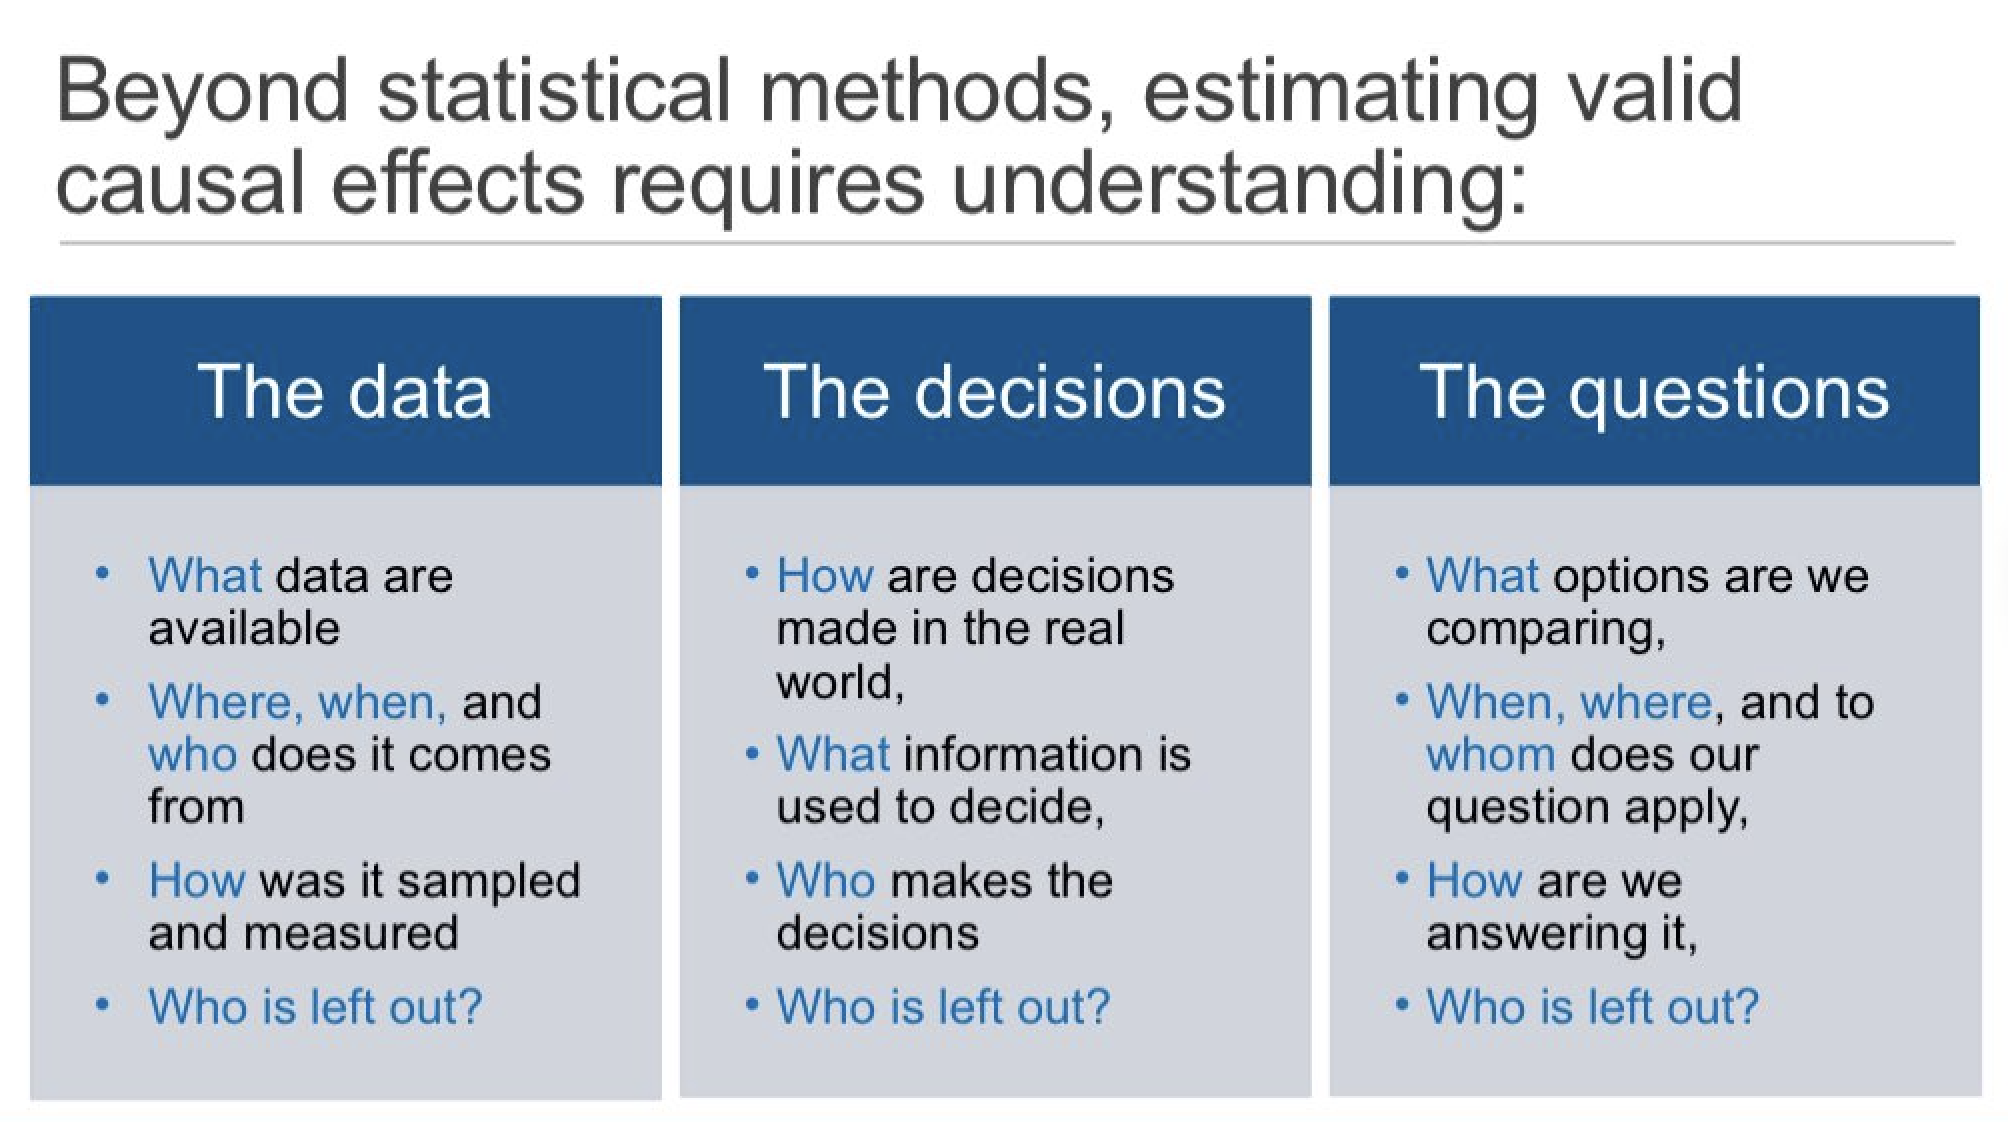
\includegraphics[width=0.75\textwidth,height=\textheight]{chapters/key_notions/../../figures/data_biases.png}

}

\caption{Tabella creata da Ellie Murray.}

\end{figure}%

È fondamentale considerare sempre i bias che influenzano la raccolta dei
dati. I dati non sono mai ``neutri'' e il loro contenuto, insieme alle
intenzioni che ne guidano la raccolta, spesso determinano
l'interpretazione che ne deriva (Nobles 2000).

Ad esempio, K. R. Johnson (2021) confronta due modalità di raccolta dati
riguardanti le persone incarcerate negli Stati Uniti: quella statale e
quella comunitaria. La raccolta dati statale si concentra su
informazioni demografiche e statistiche di base, perpetuando una
comprensione limitata e spesso distorta del sistema carcerario. Al
contrario, la raccolta dati comunitaria include dettagli più specifici
sulle condizioni di vita e gli effetti della detenzione, offrendo una
visione più completa e umana della realtà carceraria.

Negli Stati Uniti, i docenti universitari sono generalmente retribuiti
per 9 mesi all'anno. Per i restanti tre mesi, lo stipendio può essere
integrato attraverso i fondi di ricerca che il ricercatore riesce a
ottenere vincendo un grant. I grant vengono assegnati in base alla
qualità del progetto proposto e al curriculum vitae del ricercatore, in
particolare alle sue pubblicazioni. Le pubblicazioni, quindi, hanno un
impatto economico diretto per il ricercatore.

Questo crea un evidente conflitto di interesse nella conduzione della
ricerca. Immaginiamo un ricercatore noto per la sua esperienza in un
campo specifico e per aver proposto una teoria su un determinato
fenomeno. Più pubblicazioni confermeranno tale teoria, maggiori saranno
le sue possibilità di ottenere grant futuri. In questo contesto, quale
incentivo avrebbe il ricercatore a pubblicare dati che falsifichino la
teoria su cui ha costruito la sua carriera?

\section{Variabili e Costanti}\label{variabili-e-costanti}

Nell'analisi statistica, le variabili denotano le caratteristiche che
possono assumere diversi valori, sia numerici che categoriali. Le
costanti, al contrario, sono valori che non variano tra le unità di
osservazione. Le variabili indipendenti (o predittive) rappresentano i
fattori che si ipotizza influenzino l'esito di interesse, mentre le
variabili dipendenti rappresentano l'esito che si cerca di spiegare o
prevedere.

\section{Effetto}\label{effetto}

Il concetto di ``effetto'' misura il cambiamento o l'influenza tra le
variabili. Ad esempio, consideriamo uno studio che indaga l'effetto
delle mnemotecniche sul miglioramento della memoria. Se il gruppo che ha
seguito un workshop mnemonico mostra un punteggio medio superiore, si
può affermare che le mnemotecniche hanno un effetto positivo sulla
memoria. L'effetto viene misurato attraverso diverse statistiche, come
la differenza di medie o il rapporto di probabilità (Huntington-Klein
2021).

\section{Variabili Casuali}\label{variabili-casuali}

Nel contesto della teoria delle probabilità, una variabile casuale
rappresenta una quantità che può assumere diversi valori con una certa
probabilità. Dopo l'osservazione e la misurazione, una variabile casuale
diventa una variabile statistica, trasformando un'incertezza teorica in
una certezza empirica.

\section{Stima e Inferenza}\label{stima-e-inferenza}

\subsection{Stima}\label{stima}

La stima statistica permette di dedurre le caratteristiche di un'intera
popolazione partendo dall'analisi di un campione rappresentativo. Gli
elementi chiave della stima statistica sono i seguenti.

\begin{enumerate}
\def\labelenumi{\arabic{enumi}.}
\item
  Parametri della popolazione:

  \begin{itemize}
  \tightlist
  \item
    sono le caratteristiche numeriche che descrivono la popolazione;
  \item
    esempi includono la media (μ), la varianza (σ²), la proporzione (p),
    ecc.;
  \item
    generalmente non sono noti e devono essere stimati.
  \end{itemize}
\item
  Statistiche campionarie:

  \begin{itemize}
  \tightlist
  \item
    sono calcolate dai dati del campione;
  \item
    fungono da stimatori dei parametri della popolazione;
  \item
    esempi: media campionaria (x̄), varianza campionaria (s²),
    proporzione campionaria (p̂).
  \end{itemize}
\item
  Tipi di stime:

  \begin{itemize}
  \tightlist
  \item
    puntuale: fornisce un singolo valore come miglior stima del
    parametro;
  \item
    intervallare: offre un range di valori plausibili per il parametro,
    con un certo livello di credibilità o confidenza.
  \end{itemize}
\item
  Proprietà degli stimatori:

  \begin{itemize}
  \tightlist
  \item
    consistenza: la stima converge al vero valore del parametro
    all'aumentare della dimensione del campione;
  \item
    non distorsione: il valore atteso dello stimatore è uguale al vero
    valore del parametro;
  \item
    efficienza: lo stimatore ha la minor varianza possibile.
  \end{itemize}
\end{enumerate}

L'accuratezza della stima dipende da vari fattori, tra cui la dimensione
e la rappresentatività del campione, la variabilità nella popolazione e
il metodo di campionamento utilizzato.

\subsection{Inferenza Statistica}\label{inferenza-statistica}

Dopo aver ottenuto le stime iniziali, il passo successivo è l'inferenza
statistica, un processo che va oltre la semplice stima dei parametri e
permette di trarre conclusioni più generali riguardo alla popolazione di
interesse. L'inferenza statistica si concentra sulla valutazione di
ipotesi specifiche o sulla risposta a domande di ricerca basate sui dati
raccolti da un campione. In altre parole, questo ramo della statistica
si occupa di distinguere i pattern derivanti da un segnale reale
rispetto a quelli dovuti al caso.

Ad esempio, se abbiamo stimato la media del rendimento accademico in un
campione di studenti, l'inferenza statistica ci consente di quantificare
l'incertezza riguardo alla differenza di rendimento tra maschi e femmine
all'interno della popolazione più ampia. In questo modo, l'inferenza
statistica ci fornisce gli strumenti per fare previsioni e trarre
conclusioni su fenomeni che riguardano l'intera popolazione.

Esistono diversi approcci e metodologie per condurre l'inferenza
statistica, tra cui i due più comuni sono l'inferenza bayesiana e
l'approccio frequentista.

\textbf{L'inferenza bayesiana}:

\begin{itemize}
\tightlist
\item
  Si basa sul teorema di Bayes;
\item
  Utilizza probabilità a priori, che riflettono conoscenze o credenze
  iniziali su un fenomeno;
\item
  Aggiorna queste probabilità con nuovi dati per ottenere probabilità a
  posteriori;
\item
  Fornisce una interpretazione delle probabilità come gradi di credenza
  soggettivi.
\end{itemize}

\textbf{L'approccio frequentista}:

\begin{itemize}
\tightlist
\item
  Si fonda sulla frequenza relativa di eventi osservati in esperimenti
  ripetuti;
\item
  Utilizza strumenti come il test di ipotesi nulla e gli intervalli di
  confidenza per trarre conclusioni;
\item
  Non fa uso di probabilità a priori, concentrandosi esclusivamente sui
  dati osservati.
\end{itemize}

\section{Le tre sfide della
statistica}\label{le-tre-sfide-della-statistica}

Secondo Gelman, Hill, e Vehtari (2020), le tre principali sfide
dell'inferenza statistica sono:

\begin{enumerate}
\def\labelenumi{\arabic{enumi}.}
\item
  \textbf{Generalizzare dai campioni alla popolazione}: Questo problema
  è spesso associato al campionamento di comodo, una pratica comune in
  psicologia, ma che si presenta in quasi tutte le applicazioni
  dell'inferenza statistica. La sfida consiste nel trarre conclusioni
  valide su una popolazione più ampia a partire da un campione limitato.
\item
  \textbf{Generalizzare dal gruppo trattato al gruppo di controllo}:
  Questa sfida riguarda l'inferenza causale, che è una componente
  fondamentale, sia implicita che esplicita, nell'interpretazione della
  maggior parte degli studi sull'efficacia dei trattamenti psicologici.
  Si tratta di stabilire se e come i risultati osservati in un gruppo
  trattato possono essere applicati al gruppo di controllo o ad altre
  popolazioni.
\item
  \textbf{Generalizzare dalle misurazioni osservate ai costrutti
  sottostanti di interesse}: I dati raccolti in psicologia raramente
  corrispondono esattamente ai costrutti teorici che si desidera
  studiare. La sfida qui è inferire i costrutti latenti sottostanti dai
  dati osservati, che possono essere solo una rappresentazione
  imperfetta.
\end{enumerate}

Tutte e tre queste sfide possono essere interpretate come problemi di
previsione. Si tratta di fare previsioni per nuove persone o nuovi item
non inclusi nel campione, per risultati futuri in condizioni diverse
(come trattamenti differenti), e per i costrutti sottostanti di
interesse, se potessero essere misurati con maggiore precisione.

\section{Modelli Psicologici}\label{modelli-psicologici}

Un ``modello'' rappresenta una formulazione matematica semplificata di
un fenomeno reale che si desidera studiare. Si tratta di un insieme di
equazioni e ipotesi che delineano la struttura probabilistica e le
relazioni tra le variabili, cercando di catturare gli aspetti essenziali
del fenomeno senza rappresentarlo in ogni dettaglio. Poiché spesso
esistono diversi modelli che possono essere applicati allo stesso
problema, la data science si occupa dell'identificazione del modello che
meglio si adatta ai dati e che soddisfa specifici criteri di validità e
accuratezza.

I modelli psicologici sono strumenti concettuali utilizzati per
descrivere, spiegare e prevedere il comportamento umano e i processi
mentali. Un modello psicologico robusto e valido deve soddisfare diverse
caratteristiche essenziali:

\begin{enumerate}
\def\labelenumi{\arabic{enumi}.}
\tightlist
\item
  \textbf{Coerenza descrittiva}: Il modello deve fornire una
  rappresentazione logica e internamente coerente del fenomeno studiato.
  Deve catturare gli elementi essenziali del processo psicologico in
  esame, offrendo una struttura concettuale che organizzi le
  osservazioni in modo significativo e comprensibile.
\item
  \textbf{Capacità predittiva}: Un aspetto cruciale di un modello
  psicologico efficace è la sua abilità di formulare predizioni accurate
  sulle manifestazioni future del fenomeno. Questa caratteristica non
  solo aumenta l'utilità pratica del modello, ma fornisce anche un mezzo
  per testarne la validità.
\item
  \textbf{Supporto empirico}: Il modello deve essere ancorato a solide
  prove empiriche. Ciò implica che le sue assunzioni e previsioni devono
  essere confermate da dati osservabili raccolti attraverso ricerche
  sistematiche e metodologicamente rigorose.
\item
  \textbf{Falsificabilità}: Forse la caratteristica più critica, la
  falsificabilità, richiede che il modello sia costruito in modo da
  poter essere sottoposto a verifica o confutazione attraverso
  l'osservazione e l'esperimento. Questo principio, fondamentale per il
  metodo scientifico, assicura che il modello rimanga aperto al
  scrutinio critico e alla revisione basata su nuove evidenze.
\item
  \textbf{Parsimonia}: Un buon modello psicologico dovrebbe essere
  parsimonioso. Dovrebbe spiegare il fenomeno nel modo più semplice
  possibile, evitando complessità non necessarie.
\item
  \textbf{Generalizzabilità}: Il modello dovrebbe essere applicabile a
  una vasta gamma di situazioni e contesti, non solo a specifici casi o
  condizioni sperimentali.
\item
  \textbf{Utilità pratica}: Infine, un modello psicologico efficace
  dovrebbe avere implicazioni pratiche, fornendo insights utili per
  interventi, terapie o applicazioni nel mondo reale.
\end{enumerate}

La modellazione in psicologia si trova spesso di fronte a sfide uniche
dovute alla natura soggettiva e variabile dell'esperienza umana. I
ricercatori devono bilanciare la necessità di precisione scientifica con
la flessibilità richiesta per catturare la ricchezza e la complessità
dei fenomeni psicologici. Inoltre, devono essere consapevoli dei limiti
etici nella sperimentazione e delle potenziali implicazioni sociali dei
loro modelli.

La creazione e l'utilizzo di modelli in psicologia è un processo
dinamico e iterativo. I modelli sono costantemente raffinati, testati e,
se necessario, rivisti o sostituiti man mano che emergono nuove
evidenze.

L'analisi dei dati, attraverso l'applicazione di tecniche statistiche, è
il mezzo attraverso il quale un modello psicologico viene valutato.
Oltre a determinare se il modello è in grado di spiegare i dati
osservati, l'analisi può anche verificare la capacità del modello di
fare previsioni accurate su dati non ancora osservati. In questo modo,
la modellazione diventa uno strumento potente non solo per comprendere i
fenomeni psicologici ma anche per prevedere e, in alcuni casi,
influenzare il comportamento e le dinamiche mentali.

In sintesi, un modello, sia in statistica che in psicologia, è uno
strumento teorico che cerca di rappresentare un fenomeno complesso in
una forma semplificata ma informativa, guidando la comprensione, la
previsione e, in ultima analisi, l'intervento efficace su quel fenomeno.
La scelta e la valutazione del modello giusto sono fondamentali per
garantire che le conclusioni derivanti dall'analisi siano valide e utili
nel contesto specifico.

\section{Informazioni sull'Ambiente di
Sviluppo}\label{informazioni-sullambiente-di-sviluppo-8}

\begin{Shaded}
\begin{Highlighting}[]
\OperatorTok{\%}\NormalTok{load\_ext watermark}
\OperatorTok{\%}\NormalTok{watermark }\OperatorTok{{-}}\NormalTok{n }\OperatorTok{{-}}\NormalTok{u }\OperatorTok{{-}}\NormalTok{v }\OperatorTok{{-}}\NormalTok{iv }\OperatorTok{{-}}\NormalTok{w }\OperatorTok{{-}}\NormalTok{m}
\end{Highlighting}
\end{Shaded}

\begin{verbatim}
The watermark extension is already loaded. To reload it, use:
  %reload_ext watermark
Last updated: Tue Jul 23 2024

Python implementation: CPython
Python version       : 3.12.4
IPython version      : 8.26.0

Compiler    : Clang 16.0.6 
OS          : Darwin
Release     : 23.5.0
Machine     : arm64
Processor   : arm
CPU cores   : 8
Architecture: 64bit

numpy : 1.26.4
pandas: 2.2.2

Watermark: 2.4.3
\end{verbatim}

\chapter{La misurazione in psicologia}\label{sec-measurement}

\begin{quote}
Measurement, measurement, measurement. It's central to statistics. It's
central to how we learn about the world. (A. Gelman)
\end{quote}

\textbf{Prerequisiti}

\begin{itemize}
\tightlist
\item
  Leggere
  \href{https://www.sciencedirect.com/science/article/pii/S0263224115005801?casa_token=QTLWp2GIWswAAAAA:wmewUxxK68plnyJhu51VMpVSnI4rB5wB36p4l1KlKarbFwhFTuIWUS7V5ZHdfhoqSqiy4JJoqg}{On
  the philosophical foundations of psychological measurement (Maul,
  Irribarra, e Wilson 2016)} sui fondamenti filosofici della misurazione
  psicologica.
\item
  Leggere
  \href{https://web.p.ebscohost.com/ehost/pdfviewer/pdfviewer?vid=0&sid=52940ed5-6696-4f73-be23-b5f868703f25\%40redis}{Psychological
  Measurement and the Replication Crisis: Four Sacred Cows (Lilienfeld e
  Strother 2020)}. Questo articolo mette in relazione le proprietà delle
  misure psicologiche con la crisi della replicabilità dei risultati
  della ricerca.
\item
  Leggere la sezione sui numeri dell'\textbf{?@sec-numbers}.
\end{itemize}

\textbf{Concetti e competenze chiave}

\begin{itemize}
\tightlist
\item
  Conoscere le proprietà delle scale di misura di Stevens.
\item
  Comprendere quali operazioni aritmetiche possono essere applicate a
  ciascun livello di scala e perchè.
\item
  Distinguere tra variabili continue e discrete.
\item
  Capire la differenza tra accuratezza e attendibilità.
\item
  Conoscere i diversi tipi di validità e affidabilità.
\end{itemize}

\section{Introduzione}\label{introduzione-5}

La scienza si avvale di modelli per interpretare i dati, ma opera sempre
con teorie incomplete e misurazioni soggette a errori. Di conseguenza, è
fondamentale riconoscere le incertezze quando si cerca di estrarre
informazioni dalle misurazioni utilizzando i nostri modelli. Nessuna
misurazione, spiegazione o previsione è perfettamente accurata e
precisa, e non possiamo mai conoscere con esattezza l'entità dei loro
errori.

Questa incertezza viene catturata in tre equazioni fondamentali. La
prima è l'\emph{Equazione di Misurazione}, che riconosce l'errore
osservativo: \(y = z + ϵ_y\), dove \(y\) rappresenta il valore misurato,
\(z\) il valore reale e \(ϵ_y\) l'errore di misurazione. La seconda è
l'\emph{Equazione di Modellazione}, che esprime la presenza di un
diverso tipo di errore: \(z = f(x,θ) + ϵ_\text{model}\), dove \(f\) è il
modello, \(x\) sono le condizioni ambientali per cui eseguiamo il
modello, θ sono i valori dei parametri del modello e \(ϵ_\text{model}\)
rappresenta l'errore del modello, che sorge perché \(f\), \(x\) e θ
saranno tutti in qualche misura imprecisi.

Combinando queste due equazioni, otteniamo l'\emph{Equazione della
Scienza}: \(y = f(x,θ) + ϵ_\text{model} + ϵ_y\). La scienza è il
tentativo di spiegare le osservazioni \(y\) utilizzando un modello
\(f\), cercando di minimizzare l'errore di misurazione \(ϵ_y\) e
l'errore del modello \(ϵ_\text{model}\), in modo che il modello possa
essere utilizzato per fare previsioni sul mondo reale (\(z\)).
L'approccio bayesiano alla scienza riconosce e quantifica le incertezze
su tutti e sei gli elementi dell'Equazione della Scienza: \(y\), \(f\),
\(x\), θ, \(ϵ_\text{model}\) e \(ϵ_y\).

\section{La teoria della Misurazione}\label{la-teoria-della-misurazione}

La teoria della misurazione, oggetto di questo capitolo, si concentra
sull'errore di misurazione e sull'equazione fondamentale
\(y = z + ϵ_y\). Questa equazione può essere esaminata da tre
prospettive distinte. La prima concerne l'affidabilità della misura,
rappresentata dal termine \(ϵ_y\). La psicometria, branca dedicata alla
teoria della misurazione psicologica, si occupa di quantificare
l'affidabilità delle misure psicologiche attraverso metodi come la
Teoria Classica dei Test e la Teoria di Risposta all'Item.

La seconda prospettiva riguarda la validità delle misure psicologiche,
ovvero quanto adeguatamente la misura \(y\) rappresenti il costrutto
\(z\). Questo aspetto, più complesso dell'affidabilità, non può essere
risolto meramente con metodi statistici, ma richiede una profonda
comprensione delle teorie psicologiche e della loro capacità di
descrivere e prevedere i fenomeni psicologici.

La terza prospettiva si concentra sulle procedure di assegnazione dei
valori a \(y\), esplorando quali metodi (questionari, interviste,
esperimenti) siano più appropriati e come valutarne l'adeguatezza.

\subsection{Costrutti Psicologici}\label{costrutti-psicologici}

La teoria della misurazione sottolinea l'importanza di distinguere tra
la procedura di misurazione e il costrutto che si intende misurare. Ad
esempio, mentre la temperatura è un costrutto, il termometro è lo
strumento di misurazione. Analogamente, l'abilità matematica è un
costrutto, mentre un test di matematica è la procedura per misurarla.

Nelle scienze psicologiche e sociali, la misurazione presenta sfide
uniche rispetto alle scienze fisiche, poiché i costrutti in esame sono
spesso astratti e non direttamente osservabili. Ciò richiede una
particolare attenzione alla validità e all'affidabilità degli strumenti
di misurazione, nonché una costante riflessione sulle limitazioni e le
potenziali fonti di errore.

Il capitolo introduce concetti fondamentali relativi alla misurazione
quantitativa delle caratteristiche psicologiche, con un focus sulla
teoria delle scale di misura di Stevens (1946). Questa teoria fornisce
un quadro concettuale per comprendere i diversi tipi di scale di
misurazione e le operazioni matematiche appropriate per ciascuna.
Inoltre, vengono esplorate alcune procedure di scaling psicologico,
ovvero l'assegnazione di numeri all'intensità di fenomeni psicologici.

\subsection{Scaling Psicologico}\label{scaling-psicologico}

Lo scaling psicologico si occupa della trasformazione dei dati empirici
raccolti durante uno studio psicologico in misure o punteggi che
rappresentino accuratamente le caratteristiche psicologiche oggetto di
indagine.

\textbf{Scaling di Guttman.} Uno dei metodi di scaling più noti è lo
«Scaling di Guttman», che viene utilizzato per rappresentare relazioni
ordinate tra gli elementi di una scala. Ad esempio, in un questionario
sui sintomi dell'ansia, le domande possono essere disposte in ordine di
intensità crescente dei sintomi. Secondo il modello di Guttman, se un
partecipante risponde ``sì'' a una domanda che riflette un sintomo più
intenso, ci si aspetta che abbia risposto ``sì'' anche a tutte le
domande precedenti, che rappresentano sintomi di intensità minore.
Questo approccio consente di costruire una scala che riflette in modo
sistematico e coerente la gravità dei sintomi.

\textbf{Scaling Thurstoniano.} Lo «Scaling Thurstoniano» è un metodo
utilizzato per misurare preferenze o giudizi soggettivi. Ad esempio, per
valutare la preferenza tra diversi tipi di cibi, i partecipanti
confrontano due cibi alla volta ed esprimono una preferenza. Le risposte
vengono poi utilizzate per assegnare punteggi che riflettono la
preferenza media per ciascun cibo.

\textbf{Questionari Likert.} I questionari Likert richiedono ai
partecipanti di esprimere il loro grado di accordo con una serie di
affermazioni su una scala a più livelli, che va da «fortemente in
disaccordo» a «fortemente d'accordo». I punteggi ottenuti vengono
sommati per rappresentare la posizione complessiva dell'individuo
rispetto all'oggetto di studio.

\subsection{Metodi di Valutazione delle Scale
Psicologiche}\label{metodi-di-valutazione-delle-scale-psicologiche}

Per valutare le proprietà delle scale psicologiche, vengono utilizzati
vari metodi. Ad esempio, l'affidabilità delle misure può essere
analizzata utilizzando il coefficiente alpha di Cronbach o il
coefficiente Omega di McDonald, entrambi utilizzati per misurare la
coerenza interna delle risposte ai diversi item di un questionario.
Inoltre, la validità delle scale può essere esaminata confrontando i
risultati ottenuti con misure simili o attraverso analisi statistiche
che verificano se la scala cattura accuratamente il costrutto
psicologico che si intende misurare. La validità di costrutto è
particolarmente cruciale, poiché riguarda la capacità della scala di
misurare effettivamente il concetto psicologico che si intende
esplorare.

\subsection{Prospettive Moderne}\label{prospettive-moderne}

Negli ultimi anni, il dibattito sulla misurazione psicologica si è
arricchito di nuove prospettive, grazie all'avvento di tecnologie
avanzate e all'integrazione di approcci interdisciplinari. Ecco alcune
delle tendenze più rilevanti.

\textbf{Teoria della Risposta agli Item.} La Teoria della Risposta agli
Item (IRT) ha guadagnato popolarità per la sua capacità di fornire stime
più precise delle abilità latenti rispetto ai modelli classici. La IRT
considera la probabilità che un individuo risponda correttamente a un
item in funzione della sua abilità e delle caratteristiche dell'item
stesso, offrendo una visione più dettagliata delle proprietà
psicometriche degli strumenti di misurazione.

\textbf{Approcci Bayesiani.} Gli approcci bayesiani stanno
rivoluzionando il campo della psicometria, permettendo di incorporare
informazioni a priori nelle stime e di aggiornare le credenze sulla base
di nuovi dati. Questi metodi sono particolarmente utili per affrontare
la complessità e l'incertezza inerenti alla misurazione psicologica.

\textbf{Analisi di Rete.} L'analisi di rete è un'altra metodologia
emergente che vede i costrutti psicologici non come variabili latenti
indipendenti, ma come reti di sintomi interconnessi. Questo approccio
può offrire nuove intuizioni sulla struttura delle psicopatologie e
sulla dinamica dei sintomi.

\section{Le scale di misurazione}\label{le-scale-di-misurazione}

Le scale di misurazione sono strumenti fondamentali per assegnare numeri
ai dati osservati, rappresentando le proprietà psicologiche. La teoria
delle scale di Stevens Stevens (1946) identifica quattro tipi di scale
di misurazione: nominali, ordinali, a intervalli e di rapporti. Ognuna
di queste scale consente di effettuare operazioni aritmetiche diverse,
poiché ciascuna di esse è in grado di ``catturare'' solo alcune delle
proprietà dei fenomeni psicologici che si intende misurare.

\begin{figure}[H]

{\centering 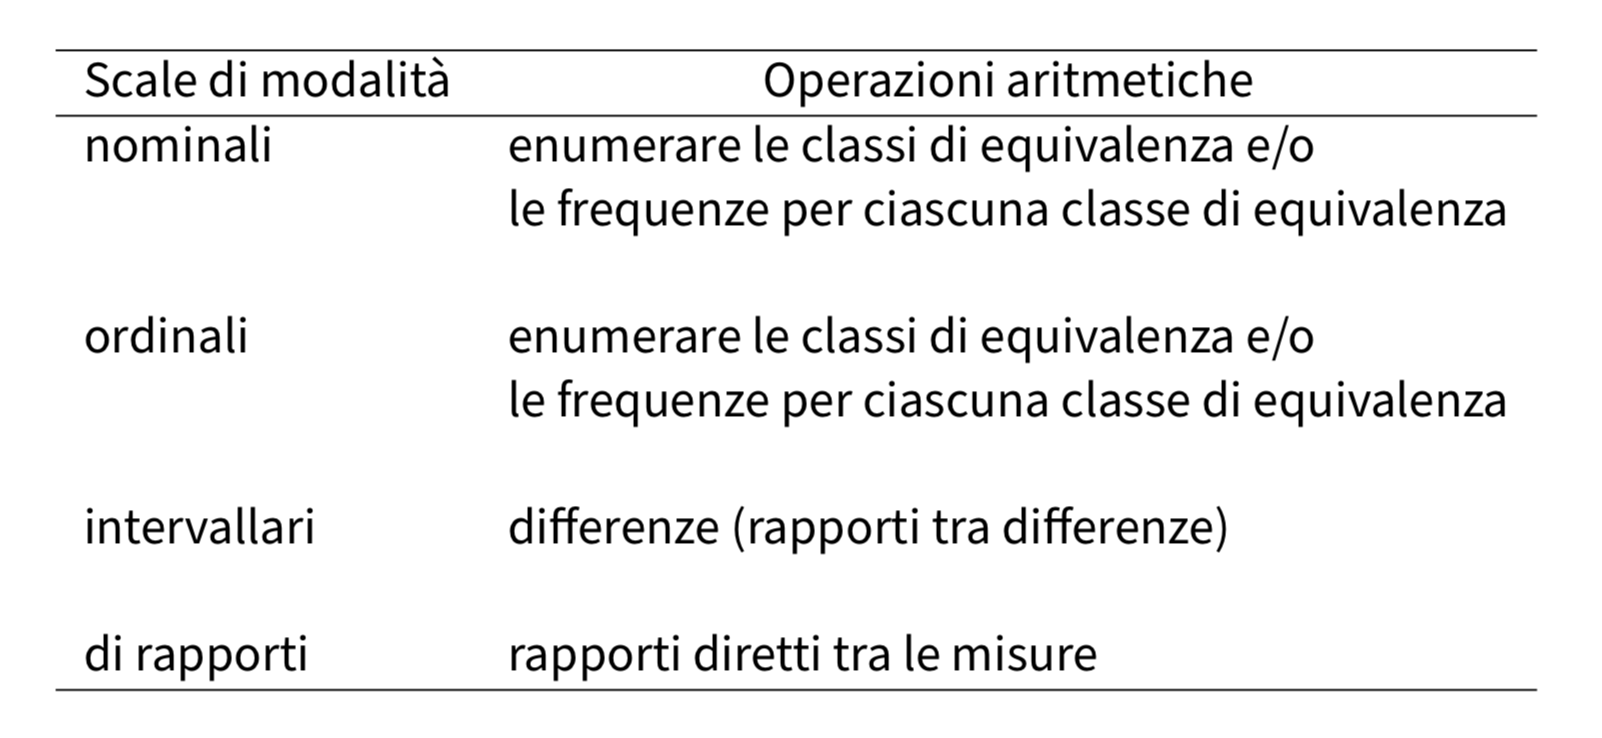
\includegraphics[width=0.7\textwidth,height=\textheight]{chapters/key_notions/../../figures/misurazione_2.png}

}

\caption{Scale di misurazione.}

\end{figure}%

\subsection{Scala nominale}\label{scala-nominale}

ILa scala nominale è il livello di misurazione più semplice e
corrisponde ad una tassonomia o classificazione delle categorie che
utilizziamo per descrivere i fenomeni psicologici. I simboli o numeri
che costituiscono questa scala rappresentano i nomi delle categorie e
non hanno alcun valore numerico intrinseco. Con la scala nominale
possiamo solo distinguere se una caratteristica psicologica è uguale o
diversa da un'altra.

I dati raccolti con la scala nominale sono suddivisi in categorie
qualitative e mutuamente esclusive, in cui ogni dato appartiene ad una
sola categoria. In questa scala, esiste solo la relazione di equivalenza
tra le misure delle unità di studio: gli elementi del campione
appartenenti a classi diverse sono differenti, mentre tutti quelli della
stessa classe sono tra loro equivalenti.

L'unica operazione algebrica consentita dalla scala nominale è quella di
contare le unità di studio che appartengono ad ogni categoria e il
numero totale di categorie. Di conseguenza, la descrizione dei dati
avviene tramite le frequenze assolute e le frequenze relative.

Dalla scala nominale è possibile costruire altre scale nominali
equivalenti alla prima, trasformando i valori della scala di partenza in
modo tale da cambiare i nomi delle categorie, ma lasciando inalterata la
suddivisione delle unità di studio nelle medesime classi di equivalenza.
In altre parole, cambiando i nomi delle categorie di una variabile
misurata su scala nominale, si ottiene una nuova variabile esattamente
equivalente alla prima.

\subsection{Scala ordinale}\label{scala-ordinale}

La scala ordinale mantiene la caratteristica della scala nominale di
classificare ogni unità di misura all'interno di una singola categoria,
ma introduce la relazione di ordinamento tra le categorie. In quanto
basata su una relazione di ordine, una scala ordinale descrive solo il
rango di ordine tra le categorie e non fornisce informazioni sulla
distanza tra di esse. Non ci dice, ad esempio, se la distanza tra le
categorie \(a\) e \(b\) è uguale, maggiore o minore della distanza tra
le categorie \(b\) e \(c\).

Un esempio classico di scala ordinale è quello della scala Mohs per la
determinazione della durezza dei minerali. Per stabilire la durezza dei
minerali si usa il criterio empirico della scalfittura. Vengono
stabiliti livelli di durezza crescente da 1 a 10 con riferimento a dieci
minerali: talco, gesso, calcite, fluorite, apatite, ortoclasio, quarzo,
topazio, corindone e diamante. Un minerale appartenente ad uno di questi
livelli se scalfisce quello di livello inferiore ed è scalfito da quello
di livello superiore.

\begin{figure}[H]

{\centering 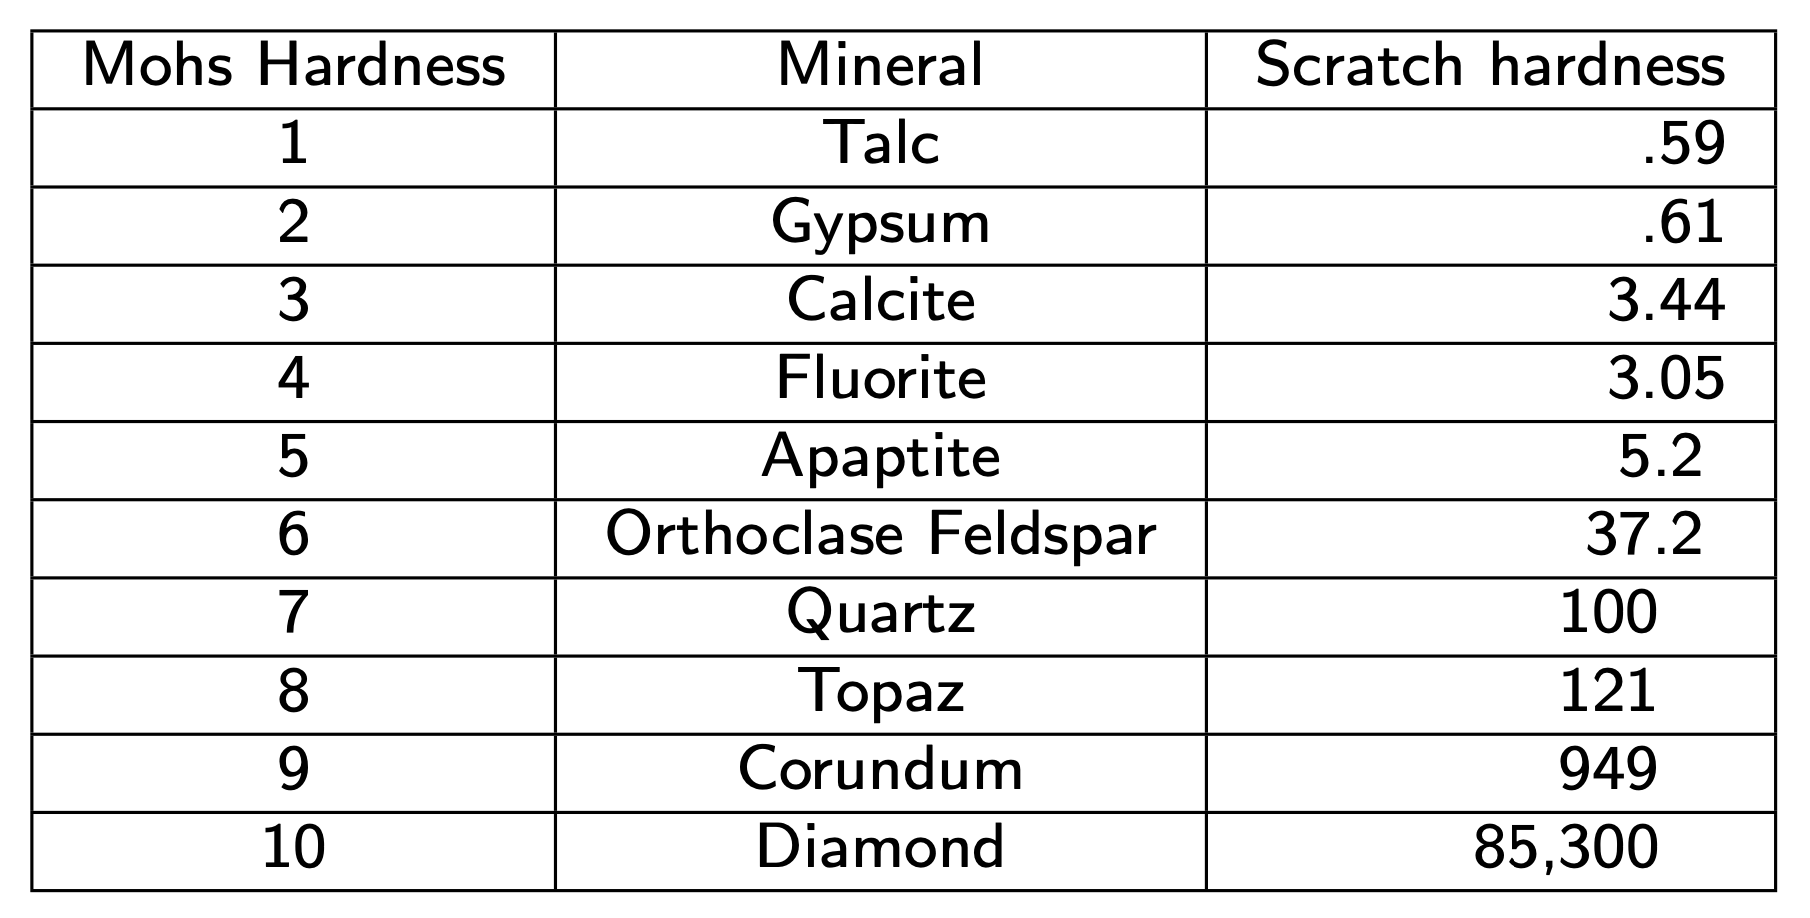
\includegraphics[width=0.62\textwidth,height=\textheight]{chapters/key_notions/../../figures/mohs.png}

}

\caption{La scala di durezza dei minerali di Mohs. Un oggetto è
considerato più duro di X se graffia X. Sono incluse anche misure di
durezza relativa utilizzando uno sclerometro, da cui emerge la non
linearità della scala di Mohs (Burchard, 2004).}

\end{figure}%

\subsection{Scala ad intervalli}\label{scala-ad-intervalli}

La scala ad intervalli di misurazione include le proprietà della scala
nominale e della scala ordinale e permette di misurare le distanze tra
le coppie di unità statistiche in termini di un intervallo costante,
chiamato ``unità di misura'', a cui viene attribuito il valore ``1''.
L'origine della scala, ovvero il punto zero, è scelta arbitrariamente e
non indica l'assenza della proprietà che si sta misurando. Ciò significa
che la scala ad intervalli consente anche valori negativi e lo zero non
viene attribuito all'unità statistica in cui la proprietà risulta
assente.

La scala ad intervalli equivalenti consente l'esecuzione di operazioni
algebriche basate sulla differenza tra i numeri associati ai diversi
punti della scala, operazioni algebriche non possibili con le scale di
misura nominale o ordinale. Tuttavia, il limite della scala ad
intervalli è che non consente di calcolare il rapporto tra coppie di
misure. È possibile affermare la differenza tra \(a\) e \(b\) come la
metà della differenza tra \(c\) e \(d\) o che le due differenze sono
uguali, ma non è possibile affermare che \(a\) abbia una proprietà
misurata in quantità doppia rispetto a \(b\). In altre parole, non è
possibile stabilire rapporti diretti tra le misure ottenute. Solo le
differenze tra le modalità permettono tutte le operazioni aritmetiche,
come la somma, l'elevazione a potenza o la divisione, che sono alla base
della statistica inferenziale.

Nelle scale ad intervalli equivalenti, l'unità di misura è arbitraria e
può essere cambiata attraverso una dilatazione, ovvero la
moltiplicazione di tutti i valori della scala per una costante positiva.
Inoltre, la traslazione, ovvero l'aggiunta di una costante a tutti i
valori della scala, è ammessa poiché non altera le differenze tra i
valori della scala. La scala rimane invariata rispetto a traslazioni e
dilatazioni e dunque le uniche trasformazioni ammissibili sono le
trasformazioni lineari:

\[
y' = a + by, \quad b > 0.
\]

Infatti, l'uguaglianza dei rapporti fra gli intervalli rimane invariata
a seguito di una trasformazione lineare.

Esempio di scala ad intervalli è la temperatura misurata in gradi
Celsius o Fahrenheit, ma non Kelvin. Come per la scala nominale, è
possibile stabilire se due modalità sono uguali o diverse: 30\(^\circ\)C
\(\neq\) 20\(^\circ\)C. Come per la scala ordinale è possibile mettere
due modalità in una relazione d'ordine: 30\(^\circ\)C \(>\)
20\(^\circ\)C. In aggiunta ai casi precedenti, però, è possibile
definire una unità di misura per cui è possibile dire che tra
30\(^\circ\)C e 20\(^\circ\)C c'è una differenza di 30\(^\circ\) -
20\(^\circ\) = 10\(^\circ\)C. I valori di temperatura, oltre a poter
essere ordinati secondo l'intensità del fenomeno, godono della proprietà
che le differenze tra loro sono direttamente confrontabili e
quantificabili.

Il limite della scala ad intervalli è quello di non consentire il
calcolo del rapporto tra coppie di misure. Ad esempio, una temperatura
di 80\(^\circ\)C non è il doppio di una di 40\(^\circ\)C. Se infatti
esprimiamo le stesse temperature nei termini della scala Fahrenheit,
allora i due valori non saranno in rapporto di 1 a 2 tra loro. Infatti,
20\(^\circ\)C = 68\(^\circ\)F e 40\(^\circ\)C = 104\(^\circ\)F. Questo
significa che la relazione ``il doppio di'' che avevamo individuato in
precedenza si applicava ai numeri della scala centigrada, ma non alla
proprietà misurata (cioè la temperatura). La decisione di che scala
usare (Centigrada vs.~Fahrenheit) è arbitraria. Ma questa arbitrarietà
non deve influenzare le inferenze che traiamo dai dati. Queste
inferenze, infatti, devono dirci qualcosa a proposito della realtà
empirica e non possono in nessun modo essere condizionate dalle nostre
scelte arbitrarie che ci portano a scegliere la scala Centigrada
piuttosto che quella Fahrenheit.

Consideriamo ora l'aspetto invariante di una trasformazione lineare,
ovvero l'uguaglianza dei rapporti fra intervalli. Prendiamo in esame, ad
esempio, tre temperature: \(20^\circ C = 68^\circ F\),
\(15^\circ C = 59^\circ F\), \(10^\circ C = 50 ^\circ F\).

È facile rendersi conto del fatto che i rapporti fra intervalli restano
costanti indipendentemente dall'unità di misura che è stata scelta:

\[
  \frac{20^\circ C - 10^\circ C}{20^\circ C - 15^\circ C} =
  \frac{68^\circ F - 50^\circ F}{68^\circ F-59^\circ F} = 2.
\]

\subsection{Scala di rapporti}\label{scala-di-rapporti}

Nella scala a rapporti equivalenti, lo zero non è arbitrario e
rappresenta l'elemento che ha intensità nulla rispetto alla proprietà
misurata. Per costruire questa scala, si associa il numero 0
all'elemento con intensità nulla e si sceglie un'unità di misura \(u\).
Ad ogni elemento si assegna un numero \(a\) definito come \(a=d/u\),
dove \(d\) rappresenta la distanza dall'origine. In questo modo, i
numeri assegnati riflettono le differenze e i rapporti tra le intensità
della proprietà misurata.

In questa scala, è possibile effettuare operazioni aritmetiche non solo
sulle differenze tra i valori della scala, ma anche sui valori stessi
della scala. L'unica scelta arbitraria è l'unità di misura, ma lo zero
deve sempre rappresentare l'intensità nulla della proprietà considerata.

Le trasformazioni ammissibili in questa scala sono chiamate
trasformazioni di similarità e sono del tipo \(y' = by\), dove \(b>0\).
In questa scala, i rapporti tra i valori rimangono invariati dopo le
trasformazioni. In altre parole, se rapportiamo due valori originali e
due valori trasformati, il rapporto rimane lo stesso:
\(\frac{y_i}{y_j} = \frac{y'_i}{y'_j}\).

\section{Gerarchia dei livelli delle scale di
misurazione}\label{gerarchia-dei-livelli-delle-scale-di-misurazione}

Secondo Stevens (1946), esiste una gerarchia dei livelli delle scale di
misurazione, denominati ``livelli di scala''. Questi livelli sono
organizzati in modo gerarchico, in cui la scala nominale rappresenta il
livello più basso della misurazione, mentre la scala a rapporti
equivalenti rappresenta il livello più alto.

\begin{itemize}
\tightlist
\item
  La scala nominale è il livello più elementare, in cui le categorie o
  le etichette vengono assegnate agli oggetti o agli individui senza
  alcuna valutazione di grandezza o ordine.
\item
  Al livello successivo si trova la scala ordinale, in cui le categorie
  sono ordinate in base a una qualche qualità o caratteristica. Qui, è
  possibile stabilire un ordine di preferenza o gerarchia tra le
  categorie, ma non è possibile quantificare la differenza tra di esse
  in modo preciso.
\item
  La scala intervallo rappresenta un livello successivo, in cui le
  categorie sono ordinate e la differenza tra di esse è quantificabile
  in modo preciso. In questa scala, è possibile effettuare operazioni
  matematiche come l'addizione e la sottrazione tra i valori, ma non è
  possibile stabilire un vero e proprio punto zero significativo.
\item
  Infine, la scala a rapporti equivalenti rappresenta il livello più
  alto. In questa scala, le categorie sono ordinate, la differenza tra
  di esse è quantificabile in modo preciso e esiste un punto zero
  assoluto che rappresenta l'assenza totale della grandezza misurata.
  Questo livello di scala permette di effettuare tutte le operazioni
  matematiche, compresa la moltiplicazione e la divisione.
\end{itemize}

Passando da un livello di misurazione ad uno più alto aumenta il numero
di operazioni aritmetiche che possono essere compiute sui valori della
scala, come indicato nella figura seguente.

\begin{figure}[H]

{\centering 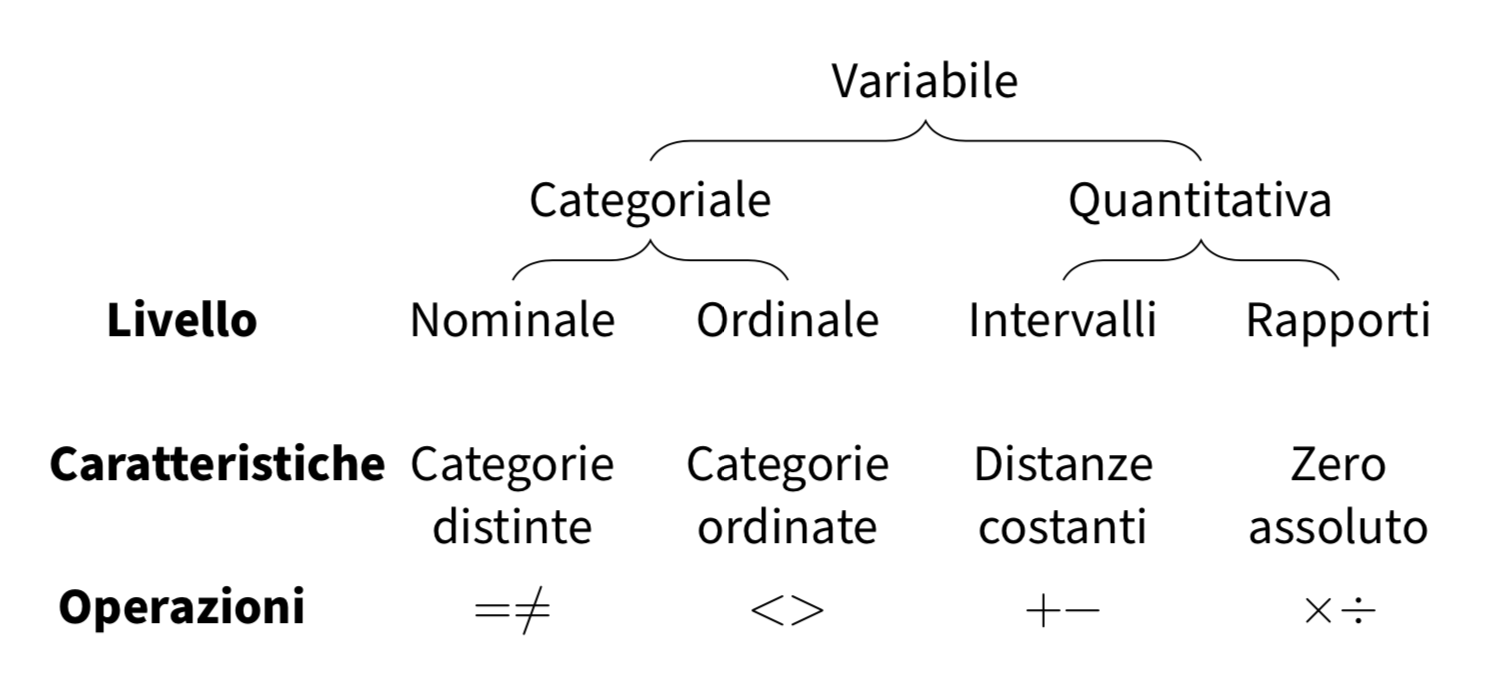
\includegraphics[width=0.65\textwidth,height=\textheight]{chapters/key_notions/../../figures/misurazione_1.png}

}

\caption{Relazioni tra i livelli di misurazione.}

\end{figure}%

Per ciò che riguarda le trasformazioni ammissibili, più il livello di
scala è basso, più le funzioni sono generali (sono minori cioè i vincoli
per passare da una rappresentazione numerica ad un'altra equivalente).
Salendo la gerarchia, la natura delle funzioni di trasformazione si fa
più restrittiva.

\section{Variabili discrete o
continue}\label{variabili-discrete-o-continue}

Le variabili possono essere classificate come variabili a livello di
intervalli o di rapporti e possono essere sia discrete che continue.

\begin{itemize}
\tightlist
\item
  Le variabili discrete assumono valori specifici ma non possono
  assumere valori intermedi. Una volta che l'elenco dei valori
  accettabili è stato definito, non vi sono casi che si trovano tra
  questi valori. In genere, le variabili discrete assumono valori
  interi, come il numero di eventi, il numero di persone o il numero di
  oggetti.
\item
  D'altra parte, le variabili continue possono assumere qualsiasi valore
  all'interno di un intervallo specificato. Teoricamente, ciò significa
  che è possibile utilizzare frazioni e decimali per ottenere qualsiasi
  grado di precisione.
\end{itemize}

\begin{figure}[H]

{\centering 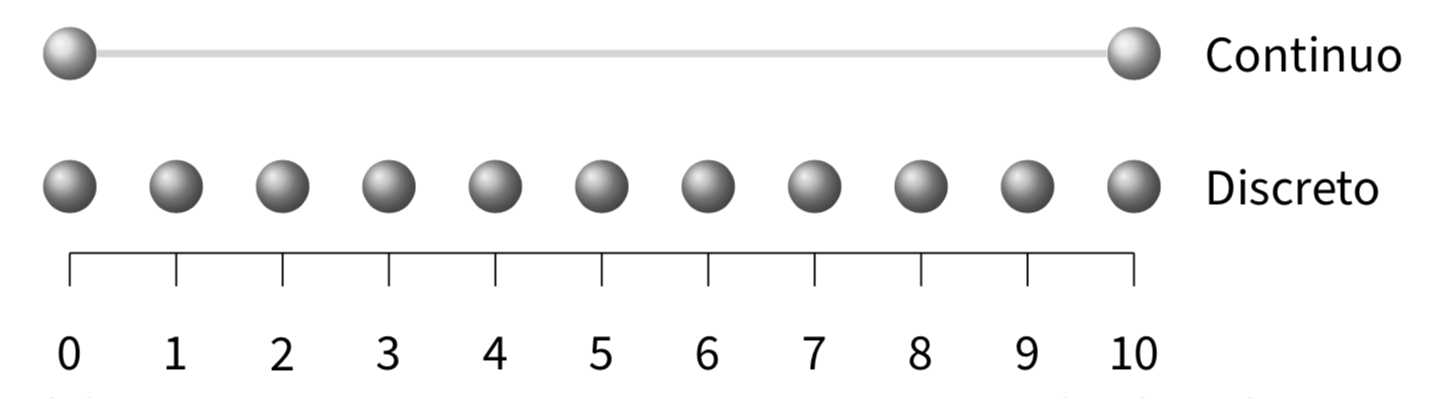
\includegraphics[width=0.65\textwidth,height=\textheight]{chapters/key_notions/../../figures/misurazione_3.png}

}

\caption{Variabili discrete e continue.}

\end{figure}%

\section{Comprendere gli errori nella
misurazione}\label{comprendere-gli-errori-nella-misurazione}

Gli errori di misurazione possono essere casuali o sistematici. Gli
errori casuali sono fluttuazioni aleatorie, mentre gli errori
sistematici sono costanti e derivano da problemi nel metodo di
misurazione o negli strumenti.

\subsection{Precisione e Accuratezza}\label{precisione-e-accuratezza}

La precisione indica la coerenza tra misurazioni ripetute, mentre
l'accuratezza si riferisce alla vicinanza del valore misurato al valore
reale. Entrambi i concetti sono cruciali per l'assessment psicometrico.

Utilizzando l'analogia del tiro al bersaglio, si può avere una serie di
colpi vicini tra loro ma lontani dal centro (precisione senza
accuratezza) oppure colpi distribuiti in modo sparso ma in media vicini
al centro (accuratezza senza precisione).

\section{Assessment psicometrico}\label{assessment-psicometrico}

L'assessment psicometrico valuta la qualità delle misurazioni
psicologiche, considerando la validità e l'affidabilità.

\subsection{Validità nella Misurazione
Psicologica}\label{validituxe0-nella-misurazione-psicologica}

La validità è una proprietà psicometrica fondamentale dei test
psicologici. Secondo gli \emph{Standards for Educational and
Psychological Testing} (2014), la validità si riferisce al grado in cui
evidenza e teoria supportano le interpretazioni dei punteggi dei test
per gli usi proposti. Questo concetto evidenzia che la validità riguarda
sia il significato dei punteggi sia il loro utilizzo, rendendola ``la
considerazione più fondamentale nello sviluppo e nella valutazione dei
test''.

\subsection{Evoluzione del Concetto di
Validità}\label{evoluzione-del-concetto-di-validituxe0}

Tradizionalmente, la validità era suddivisa in tre categorie:

\begin{itemize}
\tightlist
\item
  \textbf{Validità di Contenuto}: Si riferisce alla corrispondenza tra
  il contenuto degli item di un test e il dominio dell'attributo
  psicologico che il test intende misurare. È importante che gli item
  siano pertinenti e rappresentativi dell'attributo misurato.
\item
  \textbf{Validità di Criterio}: Valuta il grado di concordanza tra i
  risultati ottenuti tramite lo strumento di misurazione e i risultati
  ottenuti da altri strumenti che misurano lo stesso costrutto o da un
  criterio esterno. Include validità concorrente e predittiva.
\item
  \textbf{Validità di Costrutto}: Riguarda il grado in cui un test
  misura effettivamente il costrutto che si intende misurare. Si
  suddivide in validità convergente (accordo con strumenti che misurano
  lo stesso costrutto) e validità divergente (capacità di discriminare
  tra costrutti diversi).
\end{itemize}

La moderna teoria della validità non adotta più questa visione
tripartita. Gli Standards del 2014 descrivono la validità come un
concetto unitario, dove diverse forme di evidenza concorrono a
supportare l'interpretazione dei punteggi del test per il loro utilizzo
previsto.

\subsection{Tipologie di Prove di
Validità}\label{tipologie-di-prove-di-validituxe0}

Gli Standards del 2014 identificano cinque categorie principali di prove
di validità:

\begin{enumerate}
\def\labelenumi{\arabic{enumi}.}
\tightlist
\item
  \textbf{Prove Basate sul Contenuto del Test}: Valutano quanto il
  contenuto del test rappresenti adeguatamente il dominio del costrutto
  da misurare.
\item
  \textbf{Prove Basate sui Processi di Risposta}: Analizzano se i
  processi cognitivi e comportamentali degli esaminandi riflettono il
  costrutto valutato.
\item
  \textbf{Prove Basate sulla Struttura Interna}: Esaminano la coerenza
  tra gli elementi del test e la struttura teorica del costrutto.
  L'analisi fattoriale è uno strumento chiave in questo contesto.
\item
  \textbf{Prove Basate sulle Relazioni con Altre Variabili}: Studiano la
  correlazione tra i punteggi del test e altre variabili teoricamente
  correlate, utilizzando metodi come la validità convergente e
  divergente.
\item
  \textbf{Prove Basate sulle Conseguenze del Test}: Considerano le
  implicazioni e gli effetti dell'uso del test, sia intenzionali che non
  intenzionali.
\end{enumerate}

\subsection{Minacce alla Validità}\label{minacce-alla-validituxe0}

La validità può essere compromessa quando un test non misura
integralmente il costrutto di interesse (sotto-rappresentazione del
costrutto) o quando include varianza estranea al costrutto. Inoltre,
fattori esterni come l'ansia o la bassa motivazione degli esaminandi, e
deviazioni nelle procedure di amministrazione e valutazione, possono
influenzare negativamente la validità delle interpretazioni dei
risultati.

\subsection{Integrazione delle Prove di
Validità}\label{integrazione-delle-prove-di-validituxe0}

La validità di un test si costruisce attraverso l'integrazione di
diverse linee di evidenza. Ogni interpretazione o uso di un test deve
essere validato specificamente, richiedendo una valutazione continua e
accurata delle prove disponibili. Questo processo implica la costruzione
di un argomento di validità che consideri attentamente la qualità
tecnica del test e l'adeguatezza delle sue interpretazioni per gli scopi
previsti.

In conclusione, la validità è un concetto complesso e integrato che
richiede un'analisi continua e multidimensionale delle evidenze. La
moderna teoria della validità enfatizza l'importanza di considerare
diverse forme di evidenza per supportare le interpretazioni dei punteggi
dei test, garantendo che siano utilizzati in modo appropriato e
significativo. Gli sviluppatori e gli utilizzatori di test devono
impegnarsi a valutare costantemente la validità per assicurare
misurazioni psicologiche accurate e affidabili.

\subsection{Affidabilità}\label{affidabilituxe0}

L'affidabilità concerne la consistenza e stabilità delle misurazioni,
verificata attraverso metodi come l'affidabilità test-retest,
inter-rater, intra-rater e l'affidabilità interna.

\begin{itemize}
\item
  \textbf{Affidabilità Test-Retest}: Questa forma di affidabilità
  verifica la consistenza delle misurazioni nel tempo. Se un individuo
  viene testato in due momenti diversi, i risultati dovrebbero essere
  simili, assumendo che non ci siano stati cambiamenti significativi nel
  costrutto misurato.
\item
  \textbf{Affidabilità Inter-rater}: In questo caso, l'affidabilità è
  determinata dalla concordanza tra le valutazioni di diversi
  esaminatori. Ad esempio, se più psicologi dovessero valutare un
  individuo utilizzando lo stesso strumento, le loro valutazioni
  dovrebbero essere simili.
\item
  \textbf{Affidabilità Intra-rater}: Questa misura dell'affidabilità si
  riferisce alla consistenza delle valutazioni dello stesso esaminatore
  in momenti diversi.
\item
  \textbf{Affidabilità Interna}: Si riferisce alla coerenza delle
  risposte all'interno dello stesso test. Ad esempio, se un test misura
  un costrutto come l'ansia, gli item che misurano l'ansia dovrebbero
  correlare positivamente l'uno con l'altro. Un modo comune per valutare
  l'affidabilità interna è utilizzare il coefficiente \(\omega\) di
  McDonald.
\end{itemize}

\section{Commenti e considerazioni
finali}\label{commenti-e-considerazioni-finali}

La teoria della misurazione è fondamentale nella ricerca empirica per
valutare l'attendibilità e la validità delle misurazioni. È cruciale
valutare l'errore nella misurazione per garantire la precisione e
l'accuratezza delle misure. L'assessment psicometrico si occupa di
valutare la qualità delle misurazioni psicologiche, considerando
l'affidabilità e la validità per garantire misure accurate dei costrutti
teorici. Le moderne tecnologie e metodologie stanno continuamente
arricchendo questo campo, offrendo strumenti sempre più raffinati per la
comprensione delle caratteristiche psicologiche.

\chapter{L'analisi dei dati psicologici}\label{sec-scientific-method}

\textbf{Prerequisiti}

\begin{itemize}
\tightlist
\item
  Leggi \emph{Statistical Rethinking} (McElreath 2020). Focalizzati sui
  primi capitoli dove si discute della dicotomia tra ``small world'' e
  ``big world''.
\item
  Leggi
  \href{https://statmodeling.stat.columbia.edu/2016/09/21/what-has-happened-down-here-is-the-winds-have-changed/}{What
  has happened down here is the winds have changed (Gelman 2016)}. Un
  post sul blog di Andrew Gelman che fornisce una panoramica sulla crisi
  di replicazione e su come le scienze sociali sono cambiate di
  conseguenza.
\item
  Leggi
  \href{https://psycnet.apa.org/fulltext/2025-04988-001.html}{Productive
  Explanation: A Framework for Evaluating Explanations in Psychological
  Science}. L'adozione di teorie formali è essenziale per affrontare la
  crisi di riproducibilità dei risultati nella ricerca psicologica.
\item
  Per chi è interessato a un romanzo su questi temi, sorprendentemente
  avvincente, consiglio \emph{Quando abbiamo smesso di capire il mondo}
  di Benjamín Labatut (Labatut 2021).
\end{itemize}

\textbf{Concetti e competenze chiave}

\begin{itemize}
\tightlist
\item
  Emergere di ``Credibility Revolution'', ``Causal Revolution'' e
  ``Replication Crisis'' come cambiamento paradigmatico.
\item
  Proliferazione di falsi positivi, p-hacking, campioni
  sottodimensionati e mancanza di trasparenza.
\item
  Paradigma statistico che enfatizza l'aggiornamento delle priors e
  fornisce un framework flessibile per l'inferenza causale.
\item
  Interesse rinnovato nella verifica e sviluppo di modelli che superano
  la mera descrizione delle associazioni tra variabili.
\item
  Precisione, robustezza e rilevanza empirica come standard per le
  spiegazioni teoriche in psicologia.
\end{itemize}

\section*{Introduzione}\label{introduzione-6}
\addcontentsline{toc}{section}{Introduzione}

\markright{Introduzione}

Nel panorama contemporaneo delle scienze sociali e della psicologia, gli
ultimi due decenni hanno visto l'emergere di una profonda trasformazione
metodologica ed epistemologica. Questo movimento, caratterizzato da
concetti chiave quali ``Credibility Revolution'' (Angrist e Pischke
2010), ``Causal Revolution'' (Pearl e Mackenzie 2018) e ``Replication
Crisis'' (Collaboration 2015), ha determinato un cambiamento
paradigmatico nelle pratiche delle scienze sociali e, in particolare,
della psicologia (Korbmacher et al. 2023). Questa transizione verso
quella che Munger (2023) definisce ``Science versione 2'' è stata
motivata dalle lacune metodologiche precedenti e ha catalizzato
l'adozione di approcci più rigorosi e replicabili.

La genesi di questa Riforma è radicata nella constatazione di
problematiche metodologiche pervasive, tra cui la proliferazione di
falsi positivi (Simmons, Nelson, e Simonsohn 2011), l'abuso dei ``gradi
di libertà dei ricercatori'' (Gelman e Loken 2013), e l'inadeguatezza
delle pratiche statistiche tradizionali (Gelman e Loken 2014). Fenomeni
come il p-hacking, l'uso di campioni sottodimensionati (Button et al.
2013), e la mancanza di trasparenza nei metodi di ricerca hanno
contribuito a minare la credibilità delle scoperte psicologiche
(Ioannidis 2005; Meehl 1967), portando alla cosiddetta ``Replication
Crisis'' (Baker 2016; Bishop 2019) -- si veda il \textbf{?@sec-crisis}.

\section{L'Approccio Bayesiano}\label{lapproccio-bayesiano}

In risposta a queste sfide, l'approccio bayesiano è emerso come un
paradigma statistico fondamentale nella ``Credibility Revolution''.
Contrariamente all'inferenza frequentista basata sul Test dell'Ipotesi
Nulla, la statistica bayesiana offre un framework più flessibile e
intuitivo per l'analisi dei dati e l'inferenza causale. Il principio
cardine dell'approccio bayesiano, l'aggiornamento delle distribuzioni di
probabilità a priori (priors) alla luce di nuove evidenze, si allinea
perfettamente con l'obiettivo di una scienza cumulativa e
auto-correttiva.

L'adozione di metodi bayesiani in psicologia comporta diversi vantaggi
significativi:

\begin{enumerate}
\def\labelenumi{\arabic{enumi}.}
\tightlist
\item
  Quantificazione dell'incertezza: L'inferenza bayesiana fornisce
  distribuzioni di probabilità posteriori complete per i parametri di
  interesse, offrendo una rappresentazione più ricca e sfumata
  dell'incertezza rispetto agli intervalli di confidenza frequentisti.
\item
  Incorporazione di conoscenze pregresse: Le priors bayesiane consentono
  l'integrazione formale di conoscenze precedenti nel processo
  inferenziale, promuovendo un approccio cumulativo alla ricerca.
\item
  Robustezza alle pratiche di ricerca discutibili: I metodi bayesiani
  sono meno suscettibili a pratiche come il p-hacking, poiché
  l'inferenza si basa sull'intera distribuzione posteriore piuttosto che
  su soglie arbitrarie di significatività.
\end{enumerate}

\section{L'approccio bayesiano nella
ricerca}\label{lapproccio-bayesiano-nella-ricerca}

L'impiego delle statistiche bayesiane nella ricerca psicologica presenta
notevoli vantaggi rispetto ad altri metodi statistici tradizionali, come
il test di significatività dell'ipotesi nulla. Un punto di forza
importante risiede nella sua indipendenza dalla teoria dei grandi
campioni, rendendolo particolarmente adatto per gli studi psicologici
che spesso si basano su campioni di dimensioni ridotte (Larson et al.
2023).

La ricerca psicologica è frequentemente caratterizzata da campioni
limitati, dovuti a diversi fattori quali la bassa prevalenza di
determinate condizioni, le difficoltà nel reclutamento dei partecipanti
e le complessità nelle procedure di valutazione. Questi campioni di
piccole dimensioni sono intrinsecamente soggetti a una maggiore
eterogeneità, che si manifesta nella variabilità del fenotipo
comportamentale delle condizioni psicologiche esaminate e nella
discrepanza tra le stime degli effetti in diversi studi. Tale
eterogeneità può condurre a stime degli effetti distorte e scarsamente
riproducibili.

L'approccio bayesiano offre una soluzione efficace a queste
problematiche. In primo luogo, consente di valutare l'adeguatezza della
dimensione del campione attraverso un'analisi della sensibilità dei
risultati rispetto alla specificazione delle distribuzioni a priori. In
secondo luogo, permette di ottenere risultati precisi anche con campioni
ridotti, a condizione che le conoscenze a priori siano accurate e ben
definite.

Un ulteriore vantaggio dell'approccio bayesiano è la sua capacità di
ottimizzare l'uso dei campioni di partecipanti, favorendo un'inclusione
equa delle popolazioni diversificate. Questo è particolarmente rilevante
per gruppi spesso sottorappresentati, come le minoranze etniche. Le
statistiche bayesiane aiutano a superare questa sfida evitando di
esercitare una pressione eccessiva su questi gruppi per aumentarne la
partecipazione, permettendo così una ricerca più equa e rappresentativa.

\section{Modellazione Formale}\label{modellazione-formale}

La ``Credibility Revolution'' ha catalizzato l'integrazione della Data
Science nelle pratiche di ricerca psicologica. L'adozione di pipeline di
analisi dei dati riproducibili, l'uso di controllo di versione, e la
condivisione di dati e codice sono diventati standard de facto nella
comunità scientifica. Questi strumenti non solo migliorano la
trasparenza e la replicabilità della ricerca, ma facilitano anche la
collaborazione e l'accumulo di conoscenze nel campo.

Parallelamente, si è osservato un rinnovato interesse per la
modellazione formale in psicologia, che consente non solo la verifica ma
anche lo sviluppo di modelli dei meccanismi sottostanti ai fenomeni
psicologici (Oberauer e Lewandowsky 2019; Van Dongen et al. 2024).
Questo approccio supera la mera descrizione delle associazioni tra
variabili, che era tipica della pratica dominante dell'ANOVA nel
contesto pre-riforma.

La modellazione bayesiana si presta particolarmente bene a questo
approccio, offrendo un framework unificato per la specificazione di
modelli formali, l'incorporazione di incertezza parametrica, e la
valutazione dell'evidenza empirica. Attraverso tecniche come il
confronto tra modelli bayesiano e l'analisi di sensibilità, i
ricercatori possono valutare rigorosamente la plausibilità relativa di
diverse teorie psicologiche.

\section{Riflessioni Epistemologiche}\label{riflessioni-epistemologiche}

L'adozione di metodi bayesiani e della Data Science in psicologia deve
essere accompagnata da una profonda riflessione epistemologica. Come
sottolineato da George Box

\begin{quote}
tutti i modelli sono sbagliati, ma alcuni sono utili.
\end{quote}

Questa massima risuona particolarmente nel contesto della ricerca
psicologica, dove i fenomeni di interesse sono spesso complessi e
multifattoriali.

L'approccio bayesiano, con la sua enfasi sull'aggiornamento iterativo
delle credenze alla luce di nuove evidenze, si allinea naturalmente con
una visione della scienza come processo di apprendimento continuo
piuttosto che come ricerca di verità assolute. Questa prospettiva
riconosce i limiti intrinseci dei nostri modelli e delle nostre teorie,
pur valorizzandone l'utilità euristica e predittiva (si veda la
discussione nella \textbf{?@sec-poetic-validity}).

In particolare, McElreath (2020) sottolinea l'importanza di riconoscere
la dualità tra il ``mondo del modello'' e il mondo reale più ampio che
cerchiamo di comprendere. Questa consapevolezza è cruciale per evitare
la reificazione dei nostri modelli statistici e per mantenere una
prospettiva critica sulle nostre inferenze.

\section{Conclusione}\label{conclusione-1}

L'integrazione dell'approccio bayesiano e della data science nella
ricerca psicologica rappresenta una risposta promettente alle sfide
poste dalla ``Replication Crisis''. Offrendo un framework coerente per
la modellazione formale, l'inferenza statistica e l'incorporazione di
conoscenze pregresse, questi approcci promettono di elevare il rigore e
la credibilità della ricerca psicologica. Tuttavia, è fondamentale che
l'adozione di questi metodi sia accompagnata da una adeguata
consapevolezza metodologica ed epistemologica -- si veda, ad esempio, il
\textbf{?@sec-causal-inference-regr}.

\part{Epilogo}

\chapter*{Considerazioni Conclusive}\label{considerazioni-conclusive}
\addcontentsline{toc}{chapter}{Considerazioni Conclusive}

\markboth{Considerazioni Conclusive}{Considerazioni Conclusive}

L'analisi dei dati psicologici è una sfida complessa che richiede metodi
robusti e flessibili per comprendere i comportamenti umani, le emozioni
e i processi cognitivi. I metodi bayesiani offrono un potente approccio
per affrontare questa sfida, fornendo una struttura per aggiornare
continuamente le nostre ipotesi e credenze alla luce di nuovi dati.

L'approccio bayesiano parte dal principio fondamentale che la conoscenza
è costruita attraverso l'integrazione di nuove informazioni con ciò che
già sappiamo o crediamo. Questo principio è particolarmente utile in
psicologia, dove i fenomeni studiati sono spesso soggetti a incertezza e
variabilità. Le inferenze bayesiane ci permettono di incorporare
esplicitamente le conoscenze pregresse (o priori) e di aggiornare queste
conoscenze in modo quantitativo man mano che vengono raccolti nuovi
dati.

Un vantaggio dell'approccio bayesiano è la sua capacità di gestire
l'incertezza in modo naturale e intuitivo. Mentre i metodi frequentisti
tradizionali si concentrano sulle stime puntuali o sugli intervalli di
confidenza, i metodi bayesiani producono distribuzioni a posteriori
complete che descrivono interamente la credenza aggiornata riguardo a un
parametro dopo aver considerato i dati. Questo permette ai ricercatori
di comprendere meglio la gamma di valori plausibili per i parametri di
interesse e di quantificare l'incertezza associata a queste stime.

Inoltre, i metodi bayesiani sono particolarmente flessibili e possono
essere adattati a una vasta gamma di modelli e situazioni. Che si tratti
di semplici modelli lineari o di complessi modelli gerarchici,
l'approccio bayesiano consente ai ricercatori di specificare modelli che
riflettano meglio la struttura dei dati e le ipotesi di ricerca. Questa
flessibilità è cruciale in psicologia, dove i modelli di comportamento
umano spesso richiedono approcci in grado di catturare dinamiche
complesse e interazioni tra variabili.

Un altro aspetto fondamentale dell'approccio bayesiano è la trasparenza
nell'incorporazione delle ipotesi a priori. In psicologia, come in molte
altre scienze sociali, i ricercatori spesso hanno informazioni o teorie
pregresse che possono essere utilizzate per informare l'analisi dei
dati. L'approccio bayesiano permette di incorporare queste conoscenze
direttamente nel modello attraverso le distribuzioni a priori,
migliorando la validità e la rilevanza delle conclusioni derivate dai
dati.

Infine, i metodi bayesiani offrono strumenti potenti per la modellazione
predittiva. La capacità di aggiornare continuamente le credenze e di
fare previsioni basate sui dati osservati rende l'inferenza bayesiana
particolarmente utile per applicazioni che richiedono previsioni
accurate e affidabili, come la valutazione dei trattamenti psicologici o
la modellazione del comportamento umano in contesti diversi.

\section*{Limiti dell'Inferenza
Frequentista}\label{limiti-dellinferenza-frequentista}
\addcontentsline{toc}{section}{Limiti dell'Inferenza Frequentista}

\markright{Limiti dell'Inferenza Frequentista}

Nel corso di questa trattazione, abbiamo esaminato i limiti
dell'inferenza frequentista, in particolare quando viene impiegata come
``filtro'' per distinguere i risultati scientifici rilevanti da quelli
trascurabili. L'eccessiva dipendenza dai valori-p è stata oggetto di
critiche per la sua associazione con inferenze inadeguate; gli effetti
possono essere notevolmente sovrastimati, talvolta persino nella
direzione errata, quando la stima è vincolata alla significatività
statistica in presenza di dati altamente variabili (Loken e Gelman
2017).

La persistenza e la resistenza del valore-p come indicatore di
significatività sono sorprendenti, nonostante le critiche di lunga data
e i dibattiti sul suo uso improprio e sulla sua errata interpretazione
(Gardner e Altman, 1986; Cohen, 1994; Anderson et al., 2000; Fidler et
al., 2004; Finch et al., 2004). Il continuo uso di questa tenacia può
offrire spunti su come tali indici, insieme alle euristiche utilizzate
per interpretarli (ad esempio, l'assegnazione di soglie come 0.05, 0.01
e 0.001 per determinati livelli di significatività), siano adottati dai
ricercatori per ottenere una comprensione intuitiva, sebbene
eccessivamente semplificata, della struttura dei loro dati. Inoltre,
l'uso di un simile indice risulta particolarmente rilevante in contesti
che richiedono decisioni e relative giustificazioni (ad esempio, in
ambito medico).

Purtroppo, queste euristiche sono diventate estremamente rigide, e il
raggiungimento della significatività si è trasformato in un obiettivo
fine a se stesso, piuttosto che in uno strumento per comprendere i dati
(Cohen, 1994; Kirk, 1996). Ciò è particolarmente problematico
considerando che i valori-p possono essere utilizzati solo per rifiutare
l'ipotesi nulla e non per accettarla come vera, poiché un risultato
statisticamente non significativo non implica l'assenza di differenze
tra gruppi o l'assenza di un effetto di un trattamento (Wagenmakers,
2007; Amrhein et al., 2019).

I fraintendimenti e l'uso improprio dei valori-p, il cosiddetto
``p-hacking'' (Simmons et al., 2011), hanno incentivato pratiche
scientifiche discutibili, contribuendo in modo rilevante alla crisi di
riproducibilità nella scienza psicologica (Chambers et al., 2014; Szucs
e Ioannidis, 2016).

\section*{La Crisi della
Replicabilità}\label{la-crisi-della-replicabilituxe0}
\addcontentsline{toc}{section}{La Crisi della Replicabilità}

\markright{La Crisi della Replicabilità}

La crisi della replicabilità rappresenta una sfida non solo per la
ricerca psicologica, ma anche per l'applicazione pratica delle sue
teorie. Quando i risultati degli studi non possono essere replicati in
contesti diversi, si mette in dubbio la validità e l'affidabilità delle
teorie psicologiche su cui si basano gli interventi clinici e le
politiche pubbliche. Questo non solo mina la fiducia nella scienza
psicologica, ma limita anche la capacità dei professionisti di
sviluppare trattamenti efficaci e basati sull'evidenza. Pertanto, è
fondamentale che la comunità scientifica adotti pratiche di ricerca
rigorose e trasparenti per garantire che le scoperte siano replicabili e
applicabili nel mondo reale.

\section*{Come uscirne?}\label{come-uscirne}
\addcontentsline{toc}{section}{Come uscirne?}

\markright{Come uscirne?}

L'abbandono dell'inferenza frequentista a favore dei metodi bayesiani,
per ragioni quali la maggiore flessibilità, una migliore accuratezza in
presenza di dati rumorosi e campioni piccoli, una minore predisposizione
agli errori di tipo I, la possibilità di incorporare conoscenze
pregresse nell'analisi e la chiarezza e facilità di interpretazione dei
risultati (Kruschke, 2010; Kruschke et al., 2012; Etz e Vandekerckhove,
2016; Wagenmakers et al., 2016, 2018; Dienes e Mclatchie, 2018), è una
delle strategie proposte per affrontare la crisi della replicabilità
nella ricerca psicologica. Tuttavia, sebbene questo cambiamento sia
rilevante, non è sufficiente da solo. I problemi più profondi derivano
anche da un sistema accademico caratterizzato da incentivi distorti,
come la pressione a pubblicare risultati significativi, e dalla
riluttanza delle riviste scientifiche a riconoscere e affrontare casi di
frode o a ritirare articoli quando necessario.

Una proposta su cui insiste molto McElreath (2020) è quella di passare
da un approccio descrittivo della relazione tra variabili --- tipico dei
modelli lineari e dei modelli lineari generalizzati --- a una
prospettiva che miri a descrivere formalmente il meccanismo generatore
dei dati sottostante al fenomeno in esame. In questo contesto, il
ricercatore dovrebbe formulare ipotesi esplicite sul processo che genera
i dati e fornire un test quantitativo di tali ipotesi. Questo approccio
porta naturalmente alla pratica del confronto tra modelli, un metodo che
abbiamo discusso in diversi capitoli di questo testo. Tale confronto può
essere effettuato utilizzando tecniche come la validazione incrociata
bayesiana Leave-One-Out (LOO), che permette di valutare la robustezza
dei modelli e la loro capacità di generalizzare a nuovi dati. Ma si
tengano anche a mente i limiti di tale approccio (Navarro 2019).

Un altro approccio attuale per superare la cosiddetta ``junk science''
(Calin-Jageman e Caldwell 2014; Jung et al. 2014; Gelman e Weakliem
2009), che troppo spesso affligge la psicologia e non solo, è la
``rivoluzione causale''. Questo movimento si concentra sul tentativo di
comprendere e identificare le relazioni causali in contesti naturali,
superando l'arbitrarietà e l'artificialità degli esperimenti di
laboratorio tradizionali. La ``rivoluzione causale'' ha molto in comune
con l'approccio di McElreath (2020), poiché anche qui si richiede ai
ricercatori di formulare ipotesi causali in maniera esplicita e di
confrontare modelli alternativi che rappresentano diverse ipotesi sui
rapporti causali. Questo approccio non solo migliora la comprensione dei
fenomeni studiati, ma aumenta anche la credibilità e la replicabilità
dei risultati scientifici.

Questi cambiamenti prevedono anche una profonda revisione dei metodi
didattici e dei programmi dei corsi, in cui si insegna agli studenti
come formulare inferenze basate sui dati empirici raccolti in
psicologia. Questo tema è stato approfondito da studiosi come Mine
Dogucu {[}A. A. Johnson, Ott, e Dogucu (2022); dogucu2022current;
rosenberg2022making; dogucu2021web{]}. Come dovrebbe ormai essere
evidente al lettore, il presente testo ha accettato questa sfida.

\section*{Conclusioni}\label{conclusioni}
\addcontentsline{toc}{section}{Conclusioni}

\markright{Conclusioni}

L'approccio bayesiano rappresenta una risorsa fondamentale per l'analisi
dei dati psicologici, offrendo strumenti avanzati per gestire
l'incertezza, integrare conoscenze pregresse e adattarsi a modelli
complessi. La sua capacità di fornire previsioni robuste e aggiornare
continuamente le ipotesi alla luce di nuovi dati lo rende
particolarmente adatto per esplorare e comprendere la mente umana e il
comportamento in tutte le loro sfaccettature.

Tuttavia, per affrontare la crisi della replicabilità e migliorare la
qualità della ricerca scientifica in psicologia, non è sufficiente
adottare esclusivamente metodi bayesiani. È essenziale combinare questi
metodi con altre pratiche rigorose e principi metodologici solidi. Tra
queste pratiche, la formalizzazione dei modelli generativi consente di
descrivere chiaramente i processi sottostanti che generano i dati,
migliorando la trasparenza e la validità delle inferenze. Inoltre, il
confronto rigoroso tra modelli, ad esempio tramite tecniche di
validazione incrociata, aiuta a determinare quale modello meglio
rappresenta i dati e a evitare interpretazioni errate.

Infine, l'adozione di una prospettiva causale esplicita è cruciale per
identificare correttamente le relazioni di causa-effetto, evitando
l'arbitrarietà e l'artificialità degli esperimenti tradizionali. Solo
attraverso un approccio integrato, che combini l'inferenza bayesiana con
queste pratiche metodologiche avanzate, sarà possibile progredire verso
una scienza psicologica più affidabile e riproducibile, capace di
fornire una comprensione più profonda e accurata del comportamento
umano.

\bookmarksetup{startatroot}

\chapter*{Bibliografia}\label{bibliografia}
\addcontentsline{toc}{chapter}{Bibliografia}

\markboth{Bibliografia}{Bibliografia}

\phantomsection\label{refs}
\begin{CSLReferences}{1}{0}
\bibitem[\citeproctext]{ref-angrist2010credibility}
Angrist, Joshua D, e Jörn-Steffen Pischke. 2010. {«The credibility
revolution in empirical economics: How better research design is taking
the con out of econometrics»}. \emph{Journal of economic perspectives}
24 (2): 3--30.

\bibitem[\citeproctext]{ref-baker20161}
Baker, Monya. 2016. {«1,500 scientists lift the lid on
reproducibility»}. \emph{Nature} 533 (7604).

\bibitem[\citeproctext]{ref-bishop2019psychology}
Bishop, Dorothy. 2019. {«The psychology of experimental psychologists:
Overcoming cognitive constraints to improve research»}.

\bibitem[\citeproctext]{ref-button2013power}
Button, Katherine S, John PA Ioannidis, Claire Mokrysz, Brian A Nosek,
Jonathan Flint, Emma SJ Robinson, e Marcus R Munafò. 2013. {«Power
failure: why small sample size undermines the reliability of
neuroscience»}. \emph{Nature Reviews Neuroscience} 14 (5): 365--76.

\bibitem[\citeproctext]{ref-calin2014replication}
Calin-Jageman, Robert J, e Tracy L Caldwell. 2014. {«Replication of the
superstition and performance study by Damisch, Stoberock, and Mussweiler
(2010)»}. \emph{Social Psychology}.

\bibitem[\citeproctext]{ref-open2015estimating}
Collaboration, Open Science. 2015. {«Estimating the reproducibility of
psychological science»}. \emph{Science} 349 (6251): aac4716.

\bibitem[\citeproctext]{ref-definetti1970teoria}
Finetti, Bruno de. 1970. \emph{Teoria delle probabilit{à}: sintesi
introduttiva con appendice critica}. Einaudi.

\bibitem[\citeproctext]{ref-funder2014improving}
Funder, David C, John M Levine, Diane M Mackie, Carolyn C Morf, Carol
Sansone, Simine Vazire, e Stephen G West. 2014. {«Improving the
dependability of research in personality and social psychology:
Recommendations for research and educational practice»}.
\emph{Personality and Social Psychology Review} 18 (1): 3--12.

\bibitem[\citeproctext]{ref-gansch2020system}
Gansch, Roman, e Ahmad Adee. 2020. {«System theoretic view on
uncertainties»}. In \emph{2020 Design, Automation \& Test in Europe
Conference \& Exhibition (DATE)}, 1345--50. IEEE.

\bibitem[\citeproctext]{ref-gelman1995bayesian}
Gelman, Andrew, John B Carlin, Hal S Stern, e Donald B Rubin. 1995.
\emph{Bayesian data analysis}. Chapman; Hall/CRC.

\bibitem[\citeproctext]{ref-gelman2020regression}
Gelman, Andrew, Jennifer Hill, e Aki Vehtari. 2020. \emph{Regression and
Other Stories}. Cambridge University Press.

\bibitem[\citeproctext]{ref-gelman2013garden}
Gelman, Andrew, e Eric Loken. 2013. {«The garden of forking paths: Why
multiple comparisons can be a problem, even when there is no {``fishing
expedition''} or {``p-hacking''} and the research hypothesis was posited
ahead of time»}. \emph{Department of Statistics, Columbia University}
348 (1-17): 3.

\bibitem[\citeproctext]{ref-gelman2014statistical}
---------. 2014. {«The statistical crisis in science»}. \emph{American
scientist} 102 (6): 460--65.

\bibitem[\citeproctext]{ref-gelman2009beauty}
Gelman, Andrew, e David Weakliem. 2009. {«Of beauty, sex and power: Too
little attention has been paid to the statistical challenges in
estimating small effects»}. \emph{American Scientist} 97 (4): 310--16.

\bibitem[\citeproctext]{ref-huntington2021effect}
Huntington-Klein, Nick. 2021. \emph{The effect: An introduction to
research design and causality}. Chapman; Hall/CRC.

\bibitem[\citeproctext]{ref-ioannidis2005most}
Ioannidis, John PA. 2005. {«Why most published research findings are
false»}. \emph{PLoS medicine} 2 (8): e124.

\bibitem[\citeproctext]{ref-ioannidis2019have}
---------. 2019. {«What have we (not) learnt from millions of scientific
papers with P values?»} \emph{The American Statistician} 73 (sup1):
20--25.

\bibitem[\citeproctext]{ref-Johnson2022bayesrules}
Johnson, Alicia A., Miles Ott, e Mine Dogucu. 2022. \emph{{Bayes Rules!
An Introduction to Bayesian Modeling with R}}. CRC Press.

\bibitem[\citeproctext]{ref-johnson2021two}
Johnson, Kaneesha R. 2021. {«Two regimes of prison data collection»}.
\emph{Harvard Data Science Review} 3 (3): 10--1162.

\bibitem[\citeproctext]{ref-jung2014female}
Jung, Kiju, Sharon Shavitt, Madhu Viswanathan, e Joseph M Hilbe. 2014.
{«Female hurricanes are deadlier than male hurricanes»}.
\emph{Proceedings of the National Academy of Sciences} 111 (24):
8782--87.

\bibitem[\citeproctext]{ref-korbmacher2023replication}
Korbmacher, Max, Flavio Azevedo, Charlotte R Pennington, Helena
Hartmann, Madeleine Pownall, Kathleen Schmidt, Mahmoud Elsherif, et al.
2023. {«The replication crisis has led to positive structural,
procedural, and community changes»}. \emph{Communications Psychology} 1
(1): 3.

\bibitem[\citeproctext]{ref-labatut2021abbiamo}
Labatut, Benjamı́n. 2021. \emph{Quando abbiamo smesso di capire il
mondo}. Adelphi Edizioni spa.

\bibitem[\citeproctext]{ref-larson2023bayesian}
Larson, Caroline, David Kaplan, Teresa Girolamo, Sara T Kover, e
Inge-Marie Eigsti. 2023. {«A Bayesian statistics tutorial for clinical
research: Prior distributions and meaningful results for small clinical
samples»}. \emph{Journal of Clinical Psychology} 79 (11): 2602--24.

\bibitem[\citeproctext]{ref-lilienfeld2020psychological}
Lilienfeld, Scott O, e Adele N Strother. 2020. {«Psychological
measurement and the replication crisis: Four sacred cows.»}
\emph{Canadian Psychology/Psychologie Canadienne} 61 (4): 281--288.

\bibitem[\citeproctext]{ref-lindley2013understanding}
Lindley, Dennis V. 2013. \emph{Understanding uncertainty}. John Wiley \&
Sons.

\bibitem[\citeproctext]{ref-loken2017measurement}
Loken, Eric, e Andrew Gelman. 2017. {«Measurement Error and the
Replication Crisis»}. \emph{Science} 355 (6325): 584--85.

\bibitem[\citeproctext]{ref-marr2010vision}
Marr, David. 2010. \emph{Vision: A computational investigation into the
human representation and processing of visual information}. MIT press.

\bibitem[\citeproctext]{ref-Matter2025ai}
Matter, Ulrich. 2025. \emph{Data Analysis with {AI} and {R}}. 1st
Edition. New York, NY: Manning Publications.

\bibitem[\citeproctext]{ref-maul2016philosophical}
Maul, Andrew, David Torres Irribarra, e Mark Wilson. 2016. {«On the
philosophical foundations of psychological measurement»}.
\emph{Measurement} 79: 311--20.

\bibitem[\citeproctext]{ref-McElreath_rethinking}
McElreath, Richard. 2020. \emph{Statistical rethinking: {A} {Bayesian}
course with examples in {R} and {Stan}}. 2nd Edition. Boca Raton,
Florida: CRC Press.

\bibitem[\citeproctext]{ref-mckinney2022python}
McKinney, Wes. 2022. \emph{Python for Data Analysis}. " O'Reilly Media,
Inc.".

\bibitem[\citeproctext]{ref-meehl1967theory}
Meehl, Paul E. 1967. {«Theory-testing in psychology and physics: A
methodological paradox»}. \emph{Philosophy of science} 34 (2): 103--15.

\bibitem[\citeproctext]{ref-munger2023temporal}
Munger, Kevin. 2023. {«Temporal validity as meta-science»}.
\emph{Research \& Politics} 10 (3): 20531680231187271.

\bibitem[\citeproctext]{ref-murray2024measuring}
Murray, Eleanor J, e Kareem C Carr. 2024. {«Measuring Racial Sentiment
Using Social Media Is Harder Than It Seems»}. \emph{Epidemiology} 35
(1): 60--63.

\bibitem[\citeproctext]{ref-navarro2019between}
Navarro, Danielle J. 2019. {«Between the devil and the deep blue sea:
Tensions between scientific judgement and statistical model selection»}.
\emph{Computational Brain \& Behavior} 2 (1): 28--34.

\bibitem[\citeproctext]{ref-nobles2000shades}
Nobles, Melissa. 2000. \emph{Shades of citizenship: Race and the census
in modern politics}. Stanford University Press.

\bibitem[\citeproctext]{ref-oberauer2019addressing}
Oberauer, Klaus, e Stephan Lewandowsky. 2019. {«Addressing the theory
crisis in psychology»}. \emph{Psychonomic Bulletin \& Review} 26:
1596--1618.

\bibitem[\citeproctext]{ref-pearl2018book}
Pearl, Judea, e Dana Mackenzie. 2018. \emph{The book of why: the new
science of cause and effect}. Basic books.

\bibitem[\citeproctext]{ref-shrout2018psychology}
Shrout, Patrick E, e Joseph L Rodgers. 2018. {«Psychology, science, and
knowledge construction: Broadening perspectives from the replication
crisis»}. \emph{Annual Review of Psychology} 69 (1): 487--510.

\bibitem[\citeproctext]{ref-simmons2011false}
Simmons, Joseph P, Leif D Nelson, e Uri Simonsohn. 2011.
{«False-positive psychology: Undisclosed flexibility in data collection
and analysis allows presenting anything as significant»}.
\emph{Psychological science} 22 (11): 1359--66.

\bibitem[\citeproctext]{ref-stevens_46}
Stevens, Stanley Smith. 1946. {«On the theory of scales of
measurement»}. \emph{Science} 103 (2684): 677--80.

\bibitem[\citeproctext]{ref-tackett2019psychology}
Tackett, Jennifer L, Cassandra M Brandes, Kevin M King, e Kristian E
Markon. 2019. {«Psychology's replication crisis and clinical
psychological science»}. \emph{Annual Review of Clinical Psychology} 15
(1): 579--604.

\bibitem[\citeproctext]{ref-van2024productive}
Van Dongen, Noah, Riet van Bork, Adam Finnemann, Jonas Haslbeck, Han LJ
van der Maas, Donald J Robinaugh, Jill de Ron, Jan Sprenger, e Denny
Borsboom. 2024. {«Productive explanation: A framework for evaluating
explanations in psychological science.»} \emph{Psychological Review}.

\bibitem[\citeproctext]{ref-wagenmakers2018bayesian}
Wagenmakers, Eric-Jan, Maarten Marsman, Tahira Jamil, Alexander Ly,
Josine Verhagen, Jonathon Love, Ravi Selker, et al. 2018. {«Bayesian
inference for psychology. Part I: Theoretical advantages and practical
ramifications»}. \emph{Psychonomic Bulletin \& Review} 25: 35--57.

\bibitem[\citeproctext]{ref-yarkoni2022generalizability}
Yarkoni, Tal. 2022. {«The generalizability crisis»}. \emph{Behavioral
and Brain Sciences} 45: e1.

\end{CSLReferences}



\printindex


\end{document}
